\documentclass[12pt,a4paper]{book}
\usepackage{booktabs}

\usepackage[T1]{fontenc}
%\usepackage[latin1]{inputenc} % writing of äöüß possible, instead of "a"o"u"s
\usepackage[utf8]{inputenc} % for a UTF8 editor only
\usepackage{graphicx}
\usepackage{mathptmx} % font times-roman for math. Formulas, bullets, etc.
\usepackage{fancyhdr} % chapternames at top of page
\usepackage{longtable}
\usepackage{multicol}
\usepackage{sectsty}
\usepackage[ngerman,english]{babel}\selectlanguage{english}
\usepackage{makeidx} % allows for an index
\usepackage{subfigure} % enable subfigures
\usepackage[nottoc,notindex]{tocbibind} % include bib in toc
\usepackage[subfigure]{tocloft}
\usepackage{ifthen} % allow sophisticated control structures
\usepackage{substr} % allows substring detection
\usepackage{multirow}
\usepackage{array}
\usepackage{colortbl}
\usepackage{rotating}
\usepackage[nomain]{glossaries}
\usepackage{float}
\newcommand{\citep}[1]{\cite{#1}} %convenience for texmaker, but texstudio doesn't have this problem. 
\usepackage[hyphens]{url}
\usepackage[top=2cm, bottom=1.25in, left=2cm, right=2cm]{geometry}

%COLORS
\label{Color Definition}
\usepackage{xcolor}
%\definecolor{platinum}{HTML}{E5E4E2}
%\colorlet{diagrambg}{platinum}

\usepackage[colorlinks=false]{hyperref}

\makeindex

\makeglossaries

\usepackage{titlesec} % lets us format the chapters etc.

\definecolor{pinkaccent}{HTML}{F50057}


\newcommand{\mytitle}{Supporting Password Coping Strategies\\with Persuasive Design}
\newcommand{\mysubtitle}{}
\newcommand{\myname}{Tobias Seitz}
\newcommand{\ie}{i.e.,\ }
\newcommand{\eg}{e.g.,\ }

\author{\myname\\\small tobias.seitz@ifi.lmu.de}
\title{\mytitle\\
\mysubtitle\\}
\date{\today}



%Stats

\newcommand{\statslt}[3]{\textit{F\textsubscript{#1}}~$=$~#2, \textit{p}~$<$~#3}
\newcommand{\stats}[3]{\textit{F\textsubscript{#1}}~$=$~#2, \textit{p}~$=$~#3}
\newcommand{\pval}[1]{\textit{p}~$=$~#1}
\newcommand{\pvallt}[1]{\textit{p}~$<$~#1}
\newcommand{\mean}[2]{\textit{m}~$=$~#1, \textit{sd}~$=$~#2}
\newcommand{\meant}[2]{\textit{m}$=$#1 \textit{sd}$=$#2}
\newcommand{\meanonly}[1]{\textit{m}~$=$~#1}
\newcommand{\median}[1]{\textit{median}~$=$~#1}
%tables
\newcommand*{\thead}[1]{\multicolumn{1}{c}{\bfseries #1}}

%SHORTCUTS
\label{Shortcuts}
\usepackage{xspace}
\newcommand{\percent}{\%\xspace}
\newcommand{\seefig}{see Figure\xspace}
\newcommand{\red}[1]{\textcolor{red}{#1}}
\newcommand{\access}[1]{\textit{(last accessed #1)}}
\newcommand{\average}{average:\xspace}
\newcommand{\etal}{et al.\xspace}
\newcommand{\todo}[1]{\textcolor{pinkaccent}{\textbf{@@@TODO} {#1}}\ }
\newcommand{\ar}{\textcolor{pinkaccent}{\textbf{@@@TODO Add Reference}}\ }
\newcommand{\vspc}{\vspace*{2cm}} % load additional stuff
\setcounter{tocdepth}{1}
\begin{document}
	
\frontmatter
%\maketitle
\tableofcontents
\mainmatter

% ################################################### MAIN PART
%!TEX root = ../../diss.tex

\chapter[Introduction]{Introduction}\label{chap:intro}

\section{Motivation}
%% MANY PEOPLE USE THE INTERNET
Around 3.5 Billion people are using the Internet by mid-2017, i.e. about half of the world population\footnote{\url{http://www.internetworldstats.com/stats.htm}, \access{08.11.2017}}, and more than half of the households are connected to the Internet\footnote{ITU, ``Households with Internet access at home'' \url{https://de.statista.com/statistik/daten/studie/187116/umfrage/anteil-der-haushalte-mit-internetzugang/}, \access{08.11.2017}}.

%% SERVICES ARE CENTRAL TO THE INTERNET
%% MANIPULATING DATA NEEDS AUTHENTICATION
A central aspect of using the Internet is accessing the services it provides: From reading news to sharing pictures on social networks, sending emails, and doing online banking. Most of these services store data about individual users. This does not necessarily require that users interact with the data themselves. Third parties like insurance agencies, airlines, governments use the Internet to run their affairs sometimes without direct user involvement. In any case, access to sensitive data needs to be protected or else vicious attackers can exploit it. 

%However, if users can access and manipulate their private data, this usually comes along with an authentication mechanism. 
%% CONSUMER CENTRIC SERVICES ALL USE PASSWORDS
Most consumer-oriented services ask their users to register with them to access the full spectrum of the services, because in many cases access to resources is a privilege. Determining if someone can use a resource, e.g. watching a movie, requires authentication before they are authorized. User-registration is the prerequisite before any such authentication can take place, and it is a widely adopted paradigm in the online world today. For instance, from the 100 most-visited web sites in Germany, 83 offer online registration \cite{Seitz2017PoliciesReuse}, and the remaining 17 offer offline registration (e.g. banks or insurance companies, which may be required by law to perform ID checks). All of these services rely on password-based authentication. It is possible to use many of these sites without an account. Watching videos on YouTube is perfectly possible without logging in, but the full feature set is only available after the user authenticates. Thus, it is a natural to assume that users have multiple accounts. 

%% THE PERVASIVENESS OF PASSWORDS MEANS PERVASIVE PROBLEMS FOR ALL OF US
Moreover, the fact that so many websites rely on password-based authentication means that probably every single Internet user has interacted or will interact with a log-in form that prompts them for a username and password. It is a critical interaction as common as an Internet search. It requires careful interaction design to achieve both high usability and high security, which inherently generates tensions: Bad usability can lead to lower security and vice versa, but it a perfectly secure system is often unusable. 

%% HIGH LEVEL SUMMARY OF THE PROBLEM SPACE


%% HIGH LEVEL SUMMARY OF TH DESIGN SPACE
There is only so much one can do about the design and implementation of password authentication. 

in an ideal world, security teams succeed to prevent breaches. Then attacks can only focus on users. 
Fixing the User vs Fixing the System. Fixing the system: \cite{Schmidt2013Pitfalls}

%% THE DEATH PASSWORDS IS NOT AROUND THE CORNER
Password based authentication has been proclaimed to become obsolete. Some said this will happen ``over time'' (Bill Gates, 2004\footnote{\url{http://news.cnet.com/2100-1029-5164733.html}}), ``by the end of the year 2016'' \footnote{\url{https://www.theguardian.com/technology/2016/may/24/google-passwords-androidB}}. Not a month goes by without a new online article announcing that users will not need passwords anymore in the near future. In fact, the ``death of passwords'' has been declared imminent for decades \cite{Herley2012PersistenceOfPasswords, Bonneau2012ReplacePasswords}. It is perhaps not preposterous to ask whether this is really going to happen in the near future or far future. 


\subsection{Authentication Costs Time}
if you log into 3 services every day and it takes 5 seconds to type in your user name and password (\ar) you use up XX hours per year just to overcome this barriers. This is bad and we should reduce this effort. 


\subsection{Weak Passwords Cost Money}
if accounts get compromised too easily, the personal data can be exploited 

identity theft and consecutive social engineering more often than stealing money from banks.

\todo{look at reports and compile some statistics} e.g. \cite{CSID2012PasswordHabits} 

not immediately visible but important: in an enterprise environment, if employees forget passwords they often turn to the helpdesk. Handling this superfluous business costs money. 

Breachlevelindex.com \footnote{\url{http://breachlevelindex.com/}}

Cybercrime is real and getting worse \cite{BKA2016Bundeslagebild}.

\section{Research Objectives}\label{sec:intro:researchobjectives}

\subsection{Problem Statement}
investigating user interfaces that no one ``enjoys'', yet everybody needs to use them. Stobert even goes as far as to say ``Everyone hates passwords'' \cite{Stobert2014Agony}.

most security and HCI researchers agree that authentication is an unsolved problem and there have been attempts to formally show that it is unsolved \cite{Bonneau2012ReplacePasswords, Bonneau2015ImperfectAuthentication, Herley2012PersistenceOfPasswords}. 

\subsection{Better Understanding of Password Usability}
how do we make passwords more usable for mainstream users (not experts). what du users already know, what do they do and how can we design for that. 

\subsection{Making Users' Lives a Little Easier}
supporting them carefully without drastic interventions or mitigations. small steps to slowly adapt behavior over time. 


\subsection{Non-Objectives}\label{sec:intro:non_objectives}

\begin{itemize}
	\item While we present a framework to make users' dealings with passwords easier and secure for them, this thesis does not provide a definite one-size-fits-all solution to select and manage passwords. As Yang \etal put it: ``If a strategy is widely used, then attackers may develop strategy-specific methods which can efficiently guess the passwords.'' -- this increases the problem space 
\end{itemize}


\section{Main Research Contributions and Insights}\label{sec:intro:contributions}

\subsection{Insights into the Psychology of Passwords}
- personality and password selection are moderately associated
- it is difficult to measure the effects, but we show how to get there.

\subsection{Designing With Password Reuse In Mind}
- we audited the top 83 websites that offer public authentication in germany and found that their password policies (at the time) did not prevent password reuse
- we investigated users mental models of password managers and found that they are for the largest part a black box and are not trusted.

\subsection{When and Why to Apply Nudges}
- if users face a password nudge every time the effects can wear off 
- we should apply nudges if we think the account is important. important accounts contain large datasets of personal or financial information which make them valuable targets for attackers.

\subsection{Holistic Password Support}
- we propose a framework that guides service providers in making users dealings with passwords easier (the password support toolkit)
- we designed and evaluated a password manager that follows the design principles and recommendations of the password support toolkit. 

%\begin{description}
%	\item[Perception of Password Strength] Over the past decade, users received many hints and advice to construct strong passwords. Their understanding of a secure password has changed and is sometimes wrong. We show that this is the case in section @TODO REF SEC
%	
%	\item[Password Composition Policies] As many web sites require or allow some kind of registration, their operators implement different password composition policies. We show that the criteria are manifold and largely inconsistent. Consequently, users approach enrollment with their preferred password, and are forced to apply heuristics to modify the password, depending on the policy in use. 
%	
%	\item[Password Value] We present a framework to assess the value a user associates with a specific password. The users might not realize that they re-use the password for accounts with different values. Knowledge about a password's value is important to design persuasive strategies to protect it, e.g. by discouraging its usage on low value accounts. (See PST).
%\end{description}


\section{Thesis Overview}
\textbf{Part I: Background and Related Work}
\textit{Chapter 2:}
Foundations and general background on passwords
Do we still need passwords?
\textit{Chapter 3:}
Keeping the human in the loop, Usability Challenges, how users cope with password-based authentication
\textit{Chapter 4:}

\textit{Chapter 5:}

\textit{Chapter 6:}

\textit{Chapter 7:}


\section{Remarks}
\begin{itemize}
\item Throughout this dissertation pronouns are used in the plural even when speaking about an individual, e.g. ``the user'' is referred to as ``they'' instead of ``he'' or ``she'', to avoid discrimination of any demographic group. 
\item As is common in HCI literature, the author also utilizes ``We'' instead of ``I'' to acknowledge the work of any collaborators. In later more opinionated parts, the explicit usage of ``I'' intends to communicate the subjective nature of thoughts and interpretations.
\end{itemize}




\part{AUTHENTICATION ON THE WEB}
\label{part:related_work}

%%!TEX root = ../../diss.tex

\chapter[Contribution]{Contribution}\label{chap:contribution}


\section{Empiric Studies}









%%!TEX root = ../../diss.tex

\chapter[Introduction]{Introduction}\label{chap:intro}


\section{Motivation}



\section{Agenda: Claims to Support in this Thesis}

\begin{itemize}

\item[Perception of Password Strength] Over the past decade, users received many hints and advice to construct strong passwords. Their understanding of a secure password has changed and is sometimes wrong. We show that this is the case in section @TODO REF SEC

\item[Password Composition Policies] As many web sites require or allow some kind of registration, their operators implement different password composition policies. We show that the criteria are manifold and largely inconsistent. Consequently, users approach enrollment with their preferred password, and are forced to apply heuristics to modify the password, depending on the policy in use. 

\item[Password Value] We present a framework to assess the value a user associates with a specific password. The users might not realize that they re-use the password for accounts with different values. Knowledge about a password's value is important to design persuasive strategies to protect it, e.g. by discouraging its usage on low value accounts. (See PSST).

\end{itemize}


\section{Research Objectives}

\section{Research Approach}

\section{Contributions}


\section{Thesis Overview}
\textit{Chapter 1:}

\textit{Chapter 2:}

\textit{Chapter 3:}

\textit{Chapter 4:}

\textit{Chapter 5:}

\textit{Chapter 6:}

\textit{Chapter 7:}






% Background and Related Work
%!TEX root = ../../diss.tex

\chapter[Introduction]{Introduction}\label{chap:intro}

\section{Motivation}
%% MANY PEOPLE USE THE INTERNET
Around 3.5 Billion people are using the Internet by mid-2017, i.e. about half of the world population\footnote{\url{http://www.internetworldstats.com/stats.htm}, \access{08.11.2017}}, and more than half of the households are connected to the Internet\footnote{ITU, ``Households with Internet access at home'' \url{https://de.statista.com/statistik/daten/studie/187116/umfrage/anteil-der-haushalte-mit-internetzugang/}, \access{08.11.2017}}.

%% SERVICES ARE CENTRAL TO THE INTERNET
%% MANIPULATING DATA NEEDS AUTHENTICATION
A central aspect of using the Internet is accessing the services it provides: From reading news to sharing pictures on social networks, sending emails, and doing online banking. Most of these services store data about individual users. This does not necessarily require that users interact with the data themselves. Third parties like insurance agencies, airlines, governments use the Internet to run their affairs sometimes without direct user involvement. In any case, access to sensitive data needs to be protected or else vicious attackers can exploit it. 

%However, if users can access and manipulate their private data, this usually comes along with an authentication mechanism. 
%% CONSUMER CENTRIC SERVICES ALL USE PASSWORDS
Most consumer-oriented services ask their users to register with them to access the full spectrum of the services, because in many cases access to resources is a privilege. Determining if someone can use a resource, e.g. watching a movie, requires authentication before they are authorized. User-registration is the prerequisite before any such authentication can take place, and it is a widely adopted paradigm in the online world today. For instance, from the 100 most-visited web sites in Germany, 83 offer online registration \cite{Seitz2017PoliciesReuse}, and the remaining 17 offer offline registration (e.g. banks or insurance companies, which may be required by law to perform ID checks). All of these services rely on password-based authentication. It is possible to use many of these sites without an account. Watching videos on YouTube is perfectly possible without logging in, but the full feature set is only available after the user authenticates. Thus, it is a natural to assume that users have multiple accounts. 

%% THE PERVASIVENESS OF PASSWORDS MEANS PERVASIVE PROBLEMS FOR ALL OF US
Moreover, the fact that so many websites rely on password-based authentication means that probably every single Internet user has interacted or will interact with a log-in form that prompts them for a username and password. It is a critical interaction as common as an Internet search. It requires careful interaction design to achieve both high usability and high security, which inherently generates tensions: Bad usability can lead to lower security and vice versa, but it a perfectly secure system is often unusable. 

%% HIGH LEVEL SUMMARY OF THE PROBLEM SPACE


%% HIGH LEVEL SUMMARY OF TH DESIGN SPACE
There is only so much one can do about the design and implementation of password authentication. 

in an ideal world, security teams succeed to prevent breaches. Then attacks can only focus on users. 
Fixing the User vs Fixing the System. Fixing the system: \cite{Schmidt2013Pitfalls}

%% THE DEATH PASSWORDS IS NOT AROUND THE CORNER
Password based authentication has been proclaimed to become obsolete. Some said this will happen ``over time'' (Bill Gates, 2004\footnote{\url{http://news.cnet.com/2100-1029-5164733.html}}), ``by the end of the year 2016'' \footnote{\url{https://www.theguardian.com/technology/2016/may/24/google-passwords-androidB}}. Not a month goes by without a new online article announcing that users will not need passwords anymore in the near future. In fact, the ``death of passwords'' has been declared imminent for decades \cite{Herley2012PersistenceOfPasswords, Bonneau2012ReplacePasswords}. It is perhaps not preposterous to ask whether this is really going to happen in the near future or far future. 


\subsection{Authentication Costs Time}
if you log into 3 services every day and it takes 5 seconds to type in your user name and password (\ar) you use up XX hours per year just to overcome this barriers. This is bad and we should reduce this effort. 


\subsection{Weak Passwords Cost Money}
if accounts get compromised too easily, the personal data can be exploited 

identity theft and consecutive social engineering more often than stealing money from banks.

\todo{look at reports and compile some statistics} e.g. \cite{CSID2012PasswordHabits} 

not immediately visible but important: in an enterprise environment, if employees forget passwords they often turn to the helpdesk. Handling this superfluous business costs money. 

Breachlevelindex.com \footnote{\url{http://breachlevelindex.com/}}

Cybercrime is real and getting worse \cite{BKA2016Bundeslagebild}.

\section{Research Objectives}\label{sec:intro:researchobjectives}

\subsection{Problem Statement}
investigating user interfaces that no one ``enjoys'', yet everybody needs to use them. Stobert even goes as far as to say ``Everyone hates passwords'' \cite{Stobert2014Agony}.

most security and HCI researchers agree that authentication is an unsolved problem and there have been attempts to formally show that it is unsolved \cite{Bonneau2012ReplacePasswords, Bonneau2015ImperfectAuthentication, Herley2012PersistenceOfPasswords}. 

\subsection{Better Understanding of Password Usability}
how do we make passwords more usable for mainstream users (not experts). what du users already know, what do they do and how can we design for that. 

\subsection{Making Users' Lives a Little Easier}
supporting them carefully without drastic interventions or mitigations. small steps to slowly adapt behavior over time. 


\subsection{Non-Objectives}\label{sec:intro:non_objectives}

\begin{itemize}
	\item While we present a framework to make users' dealings with passwords easier and secure for them, this thesis does not provide a definite one-size-fits-all solution to select and manage passwords. As Yang \etal put it: ``If a strategy is widely used, then attackers may develop strategy-specific methods which can efficiently guess the passwords.'' -- this increases the problem space 
\end{itemize}


\section{Main Research Contributions and Insights}\label{sec:intro:contributions}

\subsection{Insights into the Psychology of Passwords}
- personality and password selection are moderately associated
- it is difficult to measure the effects, but we show how to get there.

\subsection{Designing With Password Reuse In Mind}
- we audited the top 83 websites that offer public authentication in germany and found that their password policies (at the time) did not prevent password reuse
- we investigated users mental models of password managers and found that they are for the largest part a black box and are not trusted.

\subsection{When and Why to Apply Nudges}
- if users face a password nudge every time the effects can wear off 
- we should apply nudges if we think the account is important. important accounts contain large datasets of personal or financial information which make them valuable targets for attackers.

\subsection{Holistic Password Support}
- we propose a framework that guides service providers in making users dealings with passwords easier (the password support toolkit)
- we designed and evaluated a password manager that follows the design principles and recommendations of the password support toolkit. 

%\begin{description}
%	\item[Perception of Password Strength] Over the past decade, users received many hints and advice to construct strong passwords. Their understanding of a secure password has changed and is sometimes wrong. We show that this is the case in section @TODO REF SEC
%	
%	\item[Password Composition Policies] As many web sites require or allow some kind of registration, their operators implement different password composition policies. We show that the criteria are manifold and largely inconsistent. Consequently, users approach enrollment with their preferred password, and are forced to apply heuristics to modify the password, depending on the policy in use. 
%	
%	\item[Password Value] We present a framework to assess the value a user associates with a specific password. The users might not realize that they re-use the password for accounts with different values. Knowledge about a password's value is important to design persuasive strategies to protect it, e.g. by discouraging its usage on low value accounts. (See PST).
%\end{description}


\section{Thesis Overview}
\textbf{Part I: Background and Related Work}
\textit{Chapter 2:}
Foundations and general background on passwords
Do we still need passwords?
\textit{Chapter 3:}
Keeping the human in the loop, Usability Challenges, how users cope with password-based authentication
\textit{Chapter 4:}

\textit{Chapter 5:}

\textit{Chapter 6:}

\textit{Chapter 7:}


\section{Remarks}
\begin{itemize}
\item Throughout this dissertation pronouns are used in the plural even when speaking about an individual, e.g. ``the user'' is referred to as ``they'' instead of ``he'' or ``she'', to avoid discrimination of any demographic group. 
\item As is common in HCI literature, the author also utilizes ``We'' instead of ``I'' to acknowledge the work of any collaborators. In later more opinionated parts, the explicit usage of ``I'' intends to communicate the subjective nature of thoughts and interpretations.
\end{itemize}




%!TEX root = ../../diss.tex
\chapter[Foundations]{Foundations}\label{chap:rw:passwords}
%lingo: adversaries statt attackers

% general broad description of where passwords play a role and what authentication is.
Passwords are but one puzzle piece in the realm of cyber security. They are part of the access control paradigm, which is commonly divided into three steps: identification, authentication, and authorization \cite{Riley2006IdentityAuthenticationDistinct}. Identifying a user is usually done with a prompt for a user name, so the system tries to answer the question ``who are you?''. Authentication is about proving that a user -- or more broadly an entity -- is who they claim to be, i.e. authentication is about verification of an identified entity. In other words, the system asks ``How can you prove that you are who you claim to be?''. This verification process can be based on three central elements, namely something that you know (any kind of secret), something that you are (any kind of property), or something that you have (any kind of secret token). One could argue that the second category could be extended by ``something that you do?'', e.g. provide your individual signature. However, authentication does not necessarily \textit{require} identification as a first step. It is well possible to authenticate entities even if they are anonymous. One everyday example are passwords for WiFi networks: Most of the time, the access point does not require a user name; the password, or pre-shared key, in a WPA protocol is enough to join the network. 
Last, authorization is the decision over which resources an authenticated entity is allowed to use, or an answer to ``can the user access this?''.


For this thesis, \textbf{authentication} remains the center of attention. In this chapter, we take a look at various forms of authentication and establish an argument as to why ``something that you know'' is still the most prevalent and significant authentication paradigm to date. 

\section{A Brief History of Passwords}
% first passwords were those on CTSS
The idea of protecting resources with ``something that you know'' is hundreds of years old. Think about the magic words ``open, Sesame!'' that Ali Baba spoke to enter a den used as treasury by forty thieves\footnote{Ali Baba is a fictional character in a story from ``Thousand and One Nights'' as recorded by Antoine Galland in the early 18th century. \url{http://www.pitt.edu/~dash/alibaba.html} \la{16.12.2017}}. The story already illustrates password misuse, because Ali Baba was not the rightful owner of the den and he impersonated the thieves. Nonetheless, this authentication paradigm was brought to the digital world in the early 1960s by the Massachusetts Institute of Technology (MIT) \footnote{\url{https://www.wired.com/2012/01/computer-password/}, \access{16.12.2017}}. Researchers had built a mainframe computer that was programmable by multiple users. At the time, one of the most valuable resources beside the physical device was the \textit{time} granted to use the machine. Thus, the Compatible Time Sharing System (CTSS) was conceived to give every user a certain quota of hours to operate the computer. The quota was enforced by creating user accounts that were password protected. The interaction very much resembles what we still use today: after typing the user name, the password is requested and hidden from the screen during entry.


% First flaws were evident, when the first attack happened
Shortly afterwards, the flaws of the system started to become evident when Alan Scherr became the first ``hacker''\footnote{\url{https://www.slideshare.net/CAinc/history-of-the-password/7-In_1962_a_software_bug} \la{16.12.2017}}. He desired more usage time, so he needed to impersonate other users of the computer and use their quota. The list of passwords on the system was not well protected, which allowed him to access the credentials and carry out what was probably the first password exploit in computer history. Scherr benefited from the fact that passwords were kept in plain text and could be accessed with a special punch card. Interestingly the attack was not detected immediately. Morris and Thompson mention strange behavior in their 1979 paper and blame the issue on a ``software design error'' \cite{Morris1979PasswordSecurity}, while in fact it was Scherr who was responsible for it \ar. 
% now we have cryptop
With the rise of the UNIX operating system in the 1970s, encrypted passwords became standard. The most important algorithm was the Data encryption standard (DES) which was developed by IBM and propagated by the US National Bureau of Standards (today called the National Institute of Standards and Technology, NIST) \cite{Bishop1995ProactivePasswordChecking} \ar. This algorithm was widely used until the late 1990s when computing power was sufficient to efficiently carry out attacks, which rendered DES infeasible. Luckily, the Advanced Encryption Standard had already been proposed and replaced DES. \ar
%TODO maybe add a remark about ``important'' passwords (super user / root) passwords

%TODO more cryptography ?

%%%%%% TABLE BENEFITS AND DRAWBACKS OF PASSWORDS
% Table generated by Excel2LaTeX from sheet 'Sheet1'
\begin{table}[H]
  \centering
  \caption{\label{table:rw:benefits_drawbacks_pws}Benefits and Drawbacks for different stakeholders in a password-based authentication. SPs = service providers.}
  \resizebox{\linewidth}{!}{
    \begin{tabular}{llr}
	\cmidrule{1-3}    Stakes & \textbf{Benefits} & \multicolumn{1}{l}{\textbf{Drawbacks}} \\
	\cmidrule{1-3}    \rowcolor[rgb]{ .949,  .949,  .949} \textbf{SPs} & Low costs & \multicolumn{1}{l}{Large number of attack vectors} \\
	\rowcolor[rgb]{ .949,  .949,  .949}       & Easy to implement & \multicolumn{1}{l}{Anomaly detection costly} \\
	\rowcolor[rgb]{ .949,  .949,  .949}       & Replaceable when compromised & \multicolumn{1}{l}{Attacks are simple to carry out} \\
	\rowcolor[rgb]{ .949,  .949,  .949}       & Revocable by administrator & \multicolumn{1}{l}{Attack automation simple} \\
	\rowcolor[rgb]{ .949,  .949,  .949}       & Enforceable policies & \multicolumn{1}{l}{Attacks can have severe consequences} \\
	\rowcolor[rgb]{ .886,  .937,  .855} \textbf{Users} & Fast entry on desktops & \multicolumn{1}{l}{Memory overload from too many passwords} \\
	\rowcolor[rgb]{ .886,  .937,  .855}       & Most users already familiarized & \multicolumn{1}{l}{Suboptimal coping strategies} \\
	\rowcolor[rgb]{ .886,  .937,  .855}       & Easy to learn & \multicolumn{1}{l}{Stronger passwords difficult to memorize} \\
	\rowcolor[rgb]{ .886,  .937,  .855}       & Sharable with others & \multicolumn{1}{l}{Entry on mobile devices difficult} \\
	\rowcolor[rgb]{ .886,  .937,  .855}       & High degree of control / freedom & \multicolumn{1}{l}{Mastery difficult} \\
	\rowcolor[rgb]{ .886,  .937,  .855}       &       & \multicolumn{1}{l}{Disliked by many users / perceived as burden} \\
	\rowcolor[rgb]{ .851,  .882,  .949} \textbf{Misc} & Independent of identification & \multicolumn{1}{l}{Weak passwords are a risk for users and SPs } \\
	\rowcolor[rgb]{ .851,  .882,  .949}       & Adjustable security level &  \\
	\end{tabular}%
	}%end resizebox
\end{table}%
%%%%%% 

% we were happy with what we had on the system side, so we used it a lot especially on the web.
Around 50 years after CTSS, one of its creators, Fernando Corbató, said in an interview with the Wall Street Journal that password-based authentication has ``become kind of a nightmare with the World Wide Web''\footnote{\label{foot:corbato_regrets}\url{http://on.wsj.com/1sVQOIv}, \access{18.12.2017}}. The surge of the Web has lead to many services requiring authentication. Alphanumeric passwords were the go-to solution because the system is easy to implement and has almost no set-up costs other than a database. This has led to passwords becoming the de-facto standard for authenticating users on the Web.

% passwords do have drawbacks, which is why people have started to look into ways to replace them.
However, passwords do have shortcomings for all the stakeholders involved in the authentication, e.g. Consequently, there have been many attempts to replace passwords to either minimize security risks, make things easier for the users, or -- ideally -- both at the same time. To this point, though, no alternative authentication mechanism has been able to replace alphanumeric passwords on the web, which we investigate in detail in Section \ref{sec:rw:authentication_without_pws}. Put short, the benefits provided by passwords outweigh the drawbacks most of the time. Table \ref{table:rw:benefits_drawbacks_pws} has a high-level overview of the benefits and drawbacks.


%more history in the introduction of \cite{Bishop1995ProactivePasswordChecking}, and of course as early as 1979 \cite{Morris1979PasswordSecurity}


\section{Attacks on Passwords}\label{sec:rw:attack_vectors}
As mentioned above, computer passwords were attacked shortly after they were called into action. Attacks have since become more sophisticated. In the first attack on passwords, Scherr benefited from very weak protection and was able to simply print the passwords and hack into the system. Nowadays, an attacker, or ``the bad guy'' as Morris and Thompson used to call them \cite{Morris1979PasswordSecurity}, has a number of ways to obtain a user's password(s). The following sections roughly depict how the attacks work, what the countermeasures look like, and if changing one's password behavior serves as effective countermeasure. 


%% Attack Overview Infographic
\begin{figure}[h!]
	\centering
	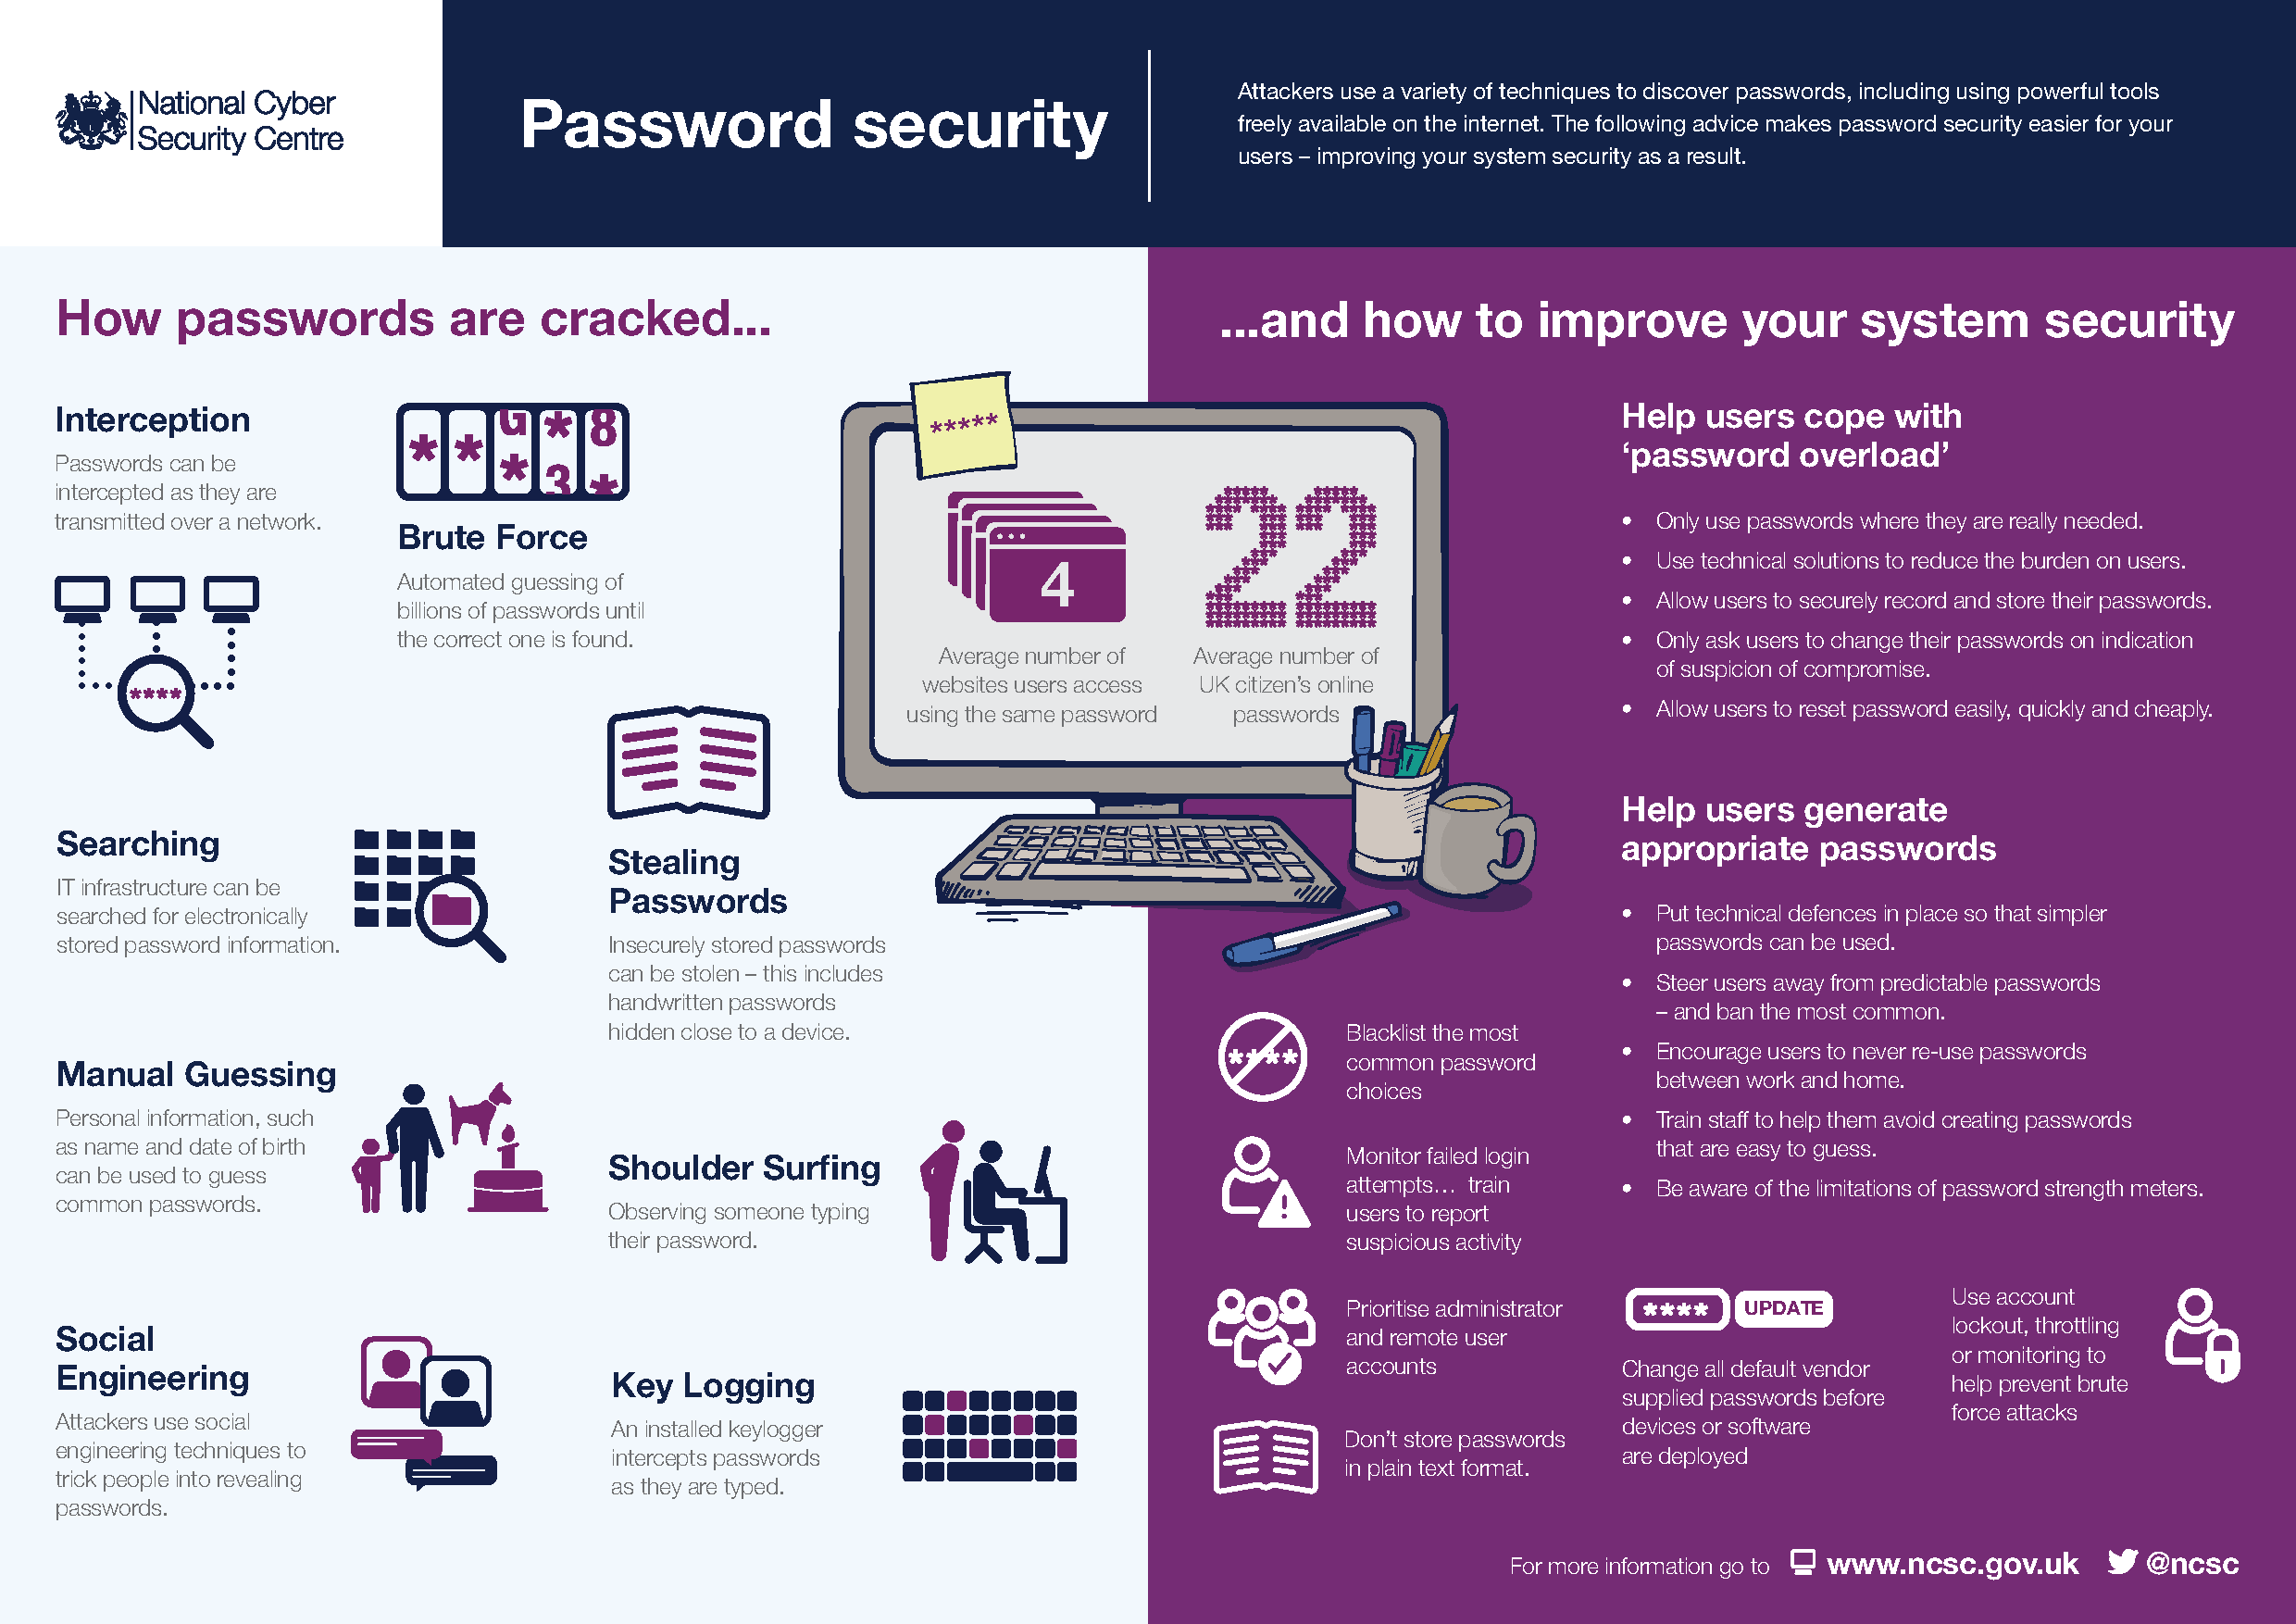
\includegraphics[width=\linewidth]{rw/NCSC-password-security-infographic}
	\caption{
		\label{fig:rw:attacks_infographic}
		Overview of attacks and high-level mitigations. Image courtesy of the National Cyber Security Centre, UK \protect\url{https://www.ncsc.gov.uk/guidance/password-collection} \protect\la{21.12.2017}
	}
\end{figure}


% A short overview of the security threats:
%%%%%%%%%%%%%%%%%%%%%%%%%%%%%%%%%%%%%%%%%
%%%%
%%%% o n l i n e    g u e s s i n g
%%%%
%%%%%%%%%%%%%%%%%%%%%%%%%%%%%%%%%%%%%%%%%
\paragraph{Online Guessing} 
%Attack description.
An adversary tries to impersonate the user by trying different combinations of user names and passwords, which are sent to the authenticating service directly. If successful, the attacker can log in without the user noticing and steal personal information, act on their behalf, and try to use the credentials on other services as well. 
% countermeasures
This attack, which is commonly known as an ``online attack'', is in many cases thwarted by throttling the number of unsuccessful login attempts per account. The service provider can lock down a user account entirely after a given number of failed login attempts. Afterwards, the user either has to manually reset their password, or they need to wait a certain time until the account is unlocked and new login attempts can be made. In the latter scenario, a strategy to hamper attacks is to implement a \textit{backoff} algorithm\footurl{https://devcentral.f5.com/articles/implementing-the-exponential-backoff-algorithm-to-thwart-dictionary-attacks}{20.12.2017} as is done in computer networks, e.g. in the Ethernet protocol \cite[p. 285]{Tanenbaum2011ComputerNetworks}. The idea behind this scheme is to (exponentially) increase the time a user (or attacker) has to wait until they can log in again after the account is locked down. Brostoff and Sasse suggest allowing ten attempts until the account is locked \cite{Brostoff2003TenStrikes}. This should give users enough trials to recover go through their list of passwords which is usually shorter than ten \cite{Florencio2007LargeScaleStudyPasswordHabits}. 
% feasibility: low, scalable but not much.
Perhaps, online guessing is only feasible for determined attackers who target specific victims, but this type of attack is not entirely uncommon \cite{Florencio2013WhereDoAllTheAttacksGo, Florencio2014PasswordPortfoliosFiniteUser, Herley2015Counterfactuals, Wang2016TargetedGuessingUnderestimated}. It is sometimes argued that such an attacker might automate up to 1 Million guesses until the attack becomes infeasible because it would simply take too long \cite{Bonneau2015ImperfectAuthentication, Florencio2014AdministratorsGuide}. However, if login attempts are not throttled, this can lead to massive attacks, like the largest attack on WordPress to date in December 2017\footurl{https://www.wordfence.com/blog/2017/12/aggressive-brute-force-wordpress-attack/}{21.12.2017}. 
% what can users do: 
Florêncio \etal argue that users are well advised to pick passwords that can at least withstand this type of attack, because it becomes too difficult to fend off offline guessing anyhow \cite{Florencio2014AdministratorsGuide, Florencio2014PasswordPortfoliosFiniteUser, Florencio2016CommACM}. 


%%%%%%%%%%%%%%%%%%%%%%%%%%%%%%%%%%%%%%%%%
%%%%
%%%% s t e a l i n g // o f f l i n e    a t t a c k s
%%%%
%%%%%%%%%%%%%%%%%%%%%%%%%%%%%%%%%%%%%%%%%
\paragraph{Stealing / Offline Guessing} Since online attacks are often impractical due to time consumption, offline attacks have prevailed in recent years\footurl{http://breachlevelindex.com/}{20.12.2017}. 
% scenario and high level description how this attack works
In this scenario an attacker breaks into the server of a service provider, usually by exploiting security holes. If this goes unnoticed, the intruder can often access the entire database containing the user account data. He or she downloads the data to their own machine, which allows them to use cracking tools like John the Ripper\footurl{http://www.openwall.com/john/}{20.12.2017}, or hashcat\footurl{https://hashcat.net/hashcat/}{20.12.2017}. These sophisticated tools use dictionaries, mangling rules and brute force to calculate password hashes which are then compared to the entry in the database. If the hashes match, the password was cracked and its plain text version is written to a file. 
% how a service provider would need to protect the data.
Optimally, the passwords in the database are salted and hashed with a slow hash function like bcrypt \cite{Provos1999bcrypt}, which drastically reduces an attacker's chances to crack the password. At the other side of the spectrum, the passwords could be stored in plain text, which would not require any cracking automation at all. Unfortunately, some of the most famous data leaks revealed that data was stored in plain text. 
% real-world examples of data breaches. first: plain text leak at RockYou
The RockYou breach in 2009 contained 32 Million user accounts for its gaming website with plain-text passwords \cite{Bonneau2012ScienceOfGuessing, Weir2010MetricsPolicies}. At the time, RockYou developed games for MySpace and Facebook and the database also contained credentials for these sites\footurl{https://techcrunch.com/2009/12/14/rockyou-hack-security-myspace-facebook-passwords/}{20.12.2017}, which made the leak even more severe. Strong passwords would not have helped at all to avoid losing personal data. Perhaps RockYou's loose policy (5 characters) helped in safeguarding other accounts where more complex policies were in place, because users were not able to reuse their RockYou password there. 
% hashed leaks
In other instances of stolen password databases, the passwords were indeed hashed, e.g. the infamous LinkedIn breaches\footurl{http://fortune.com/2016/05/18/linkedin-data-breach-email-password/}{20.12.2017} -- again with millions of rows of user data \cite{Huh2017TooBusy}. 
% User perspective: it's hard or nearly impossible. 
Users are challenged to find a password that withstands this kind of attack. The large issue is that attackers are basically only limited by the time they want to spend calculating password hashes \cite{Block2017EconomicsOfflineCracking}. On modern machines with a single GPU, thousands of hashes can be calculated per second even for slow algorithms\footurl{https://gist.github.com/epixoip/9d9b943fd580ff6bfa80e48a0e77520d}{20.12.2017}. Perhaps, this is why Florêncio \etal argue that it is futile to encourage users to pick a password that would withstand such an attack \cite{Florencio2014AdministratorsGuide, Florencio2016CommACM}. 
%TODO what happens after a breach?

%% PHISHING WEBSITE SCREENSHOT
\begin{figure}[h!]
	\centering
	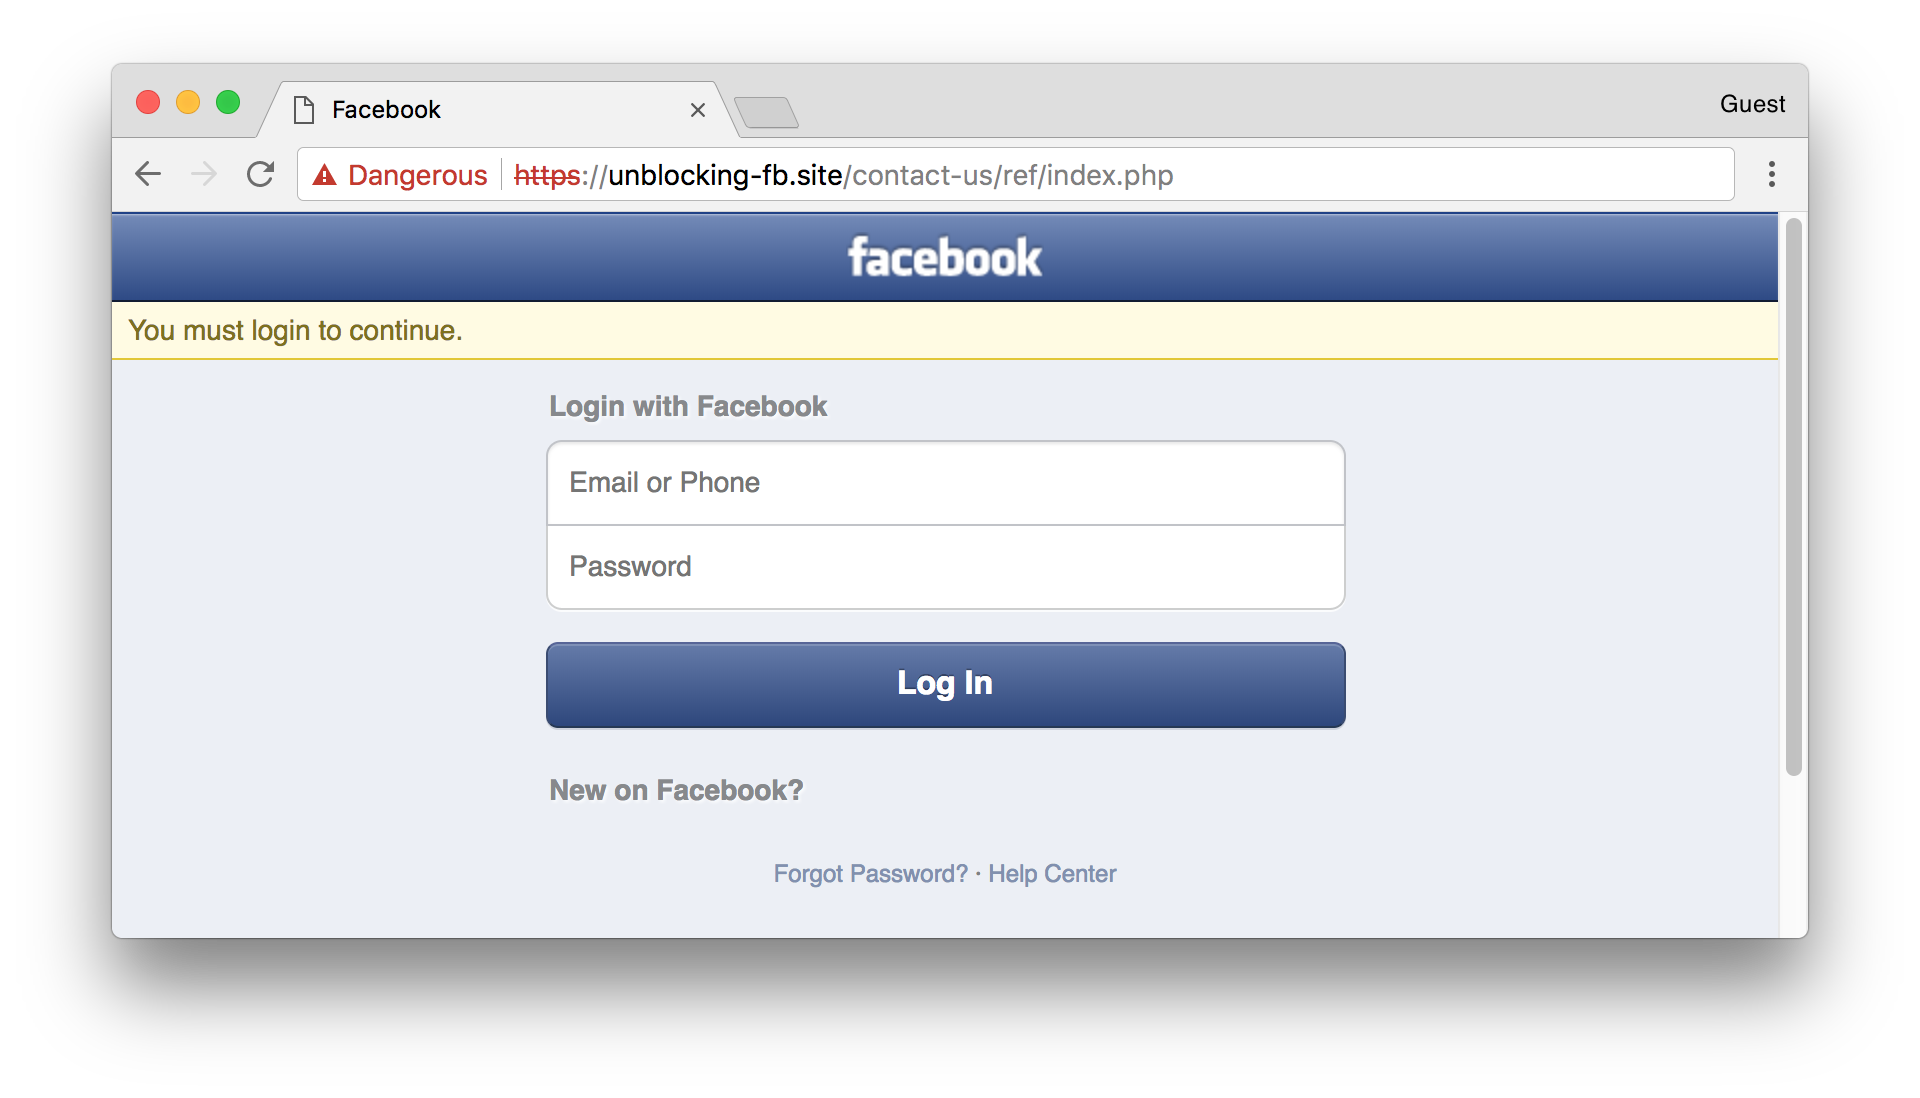
\includegraphics[width=0.7\linewidth]{rw/facebook-phishing-site}
	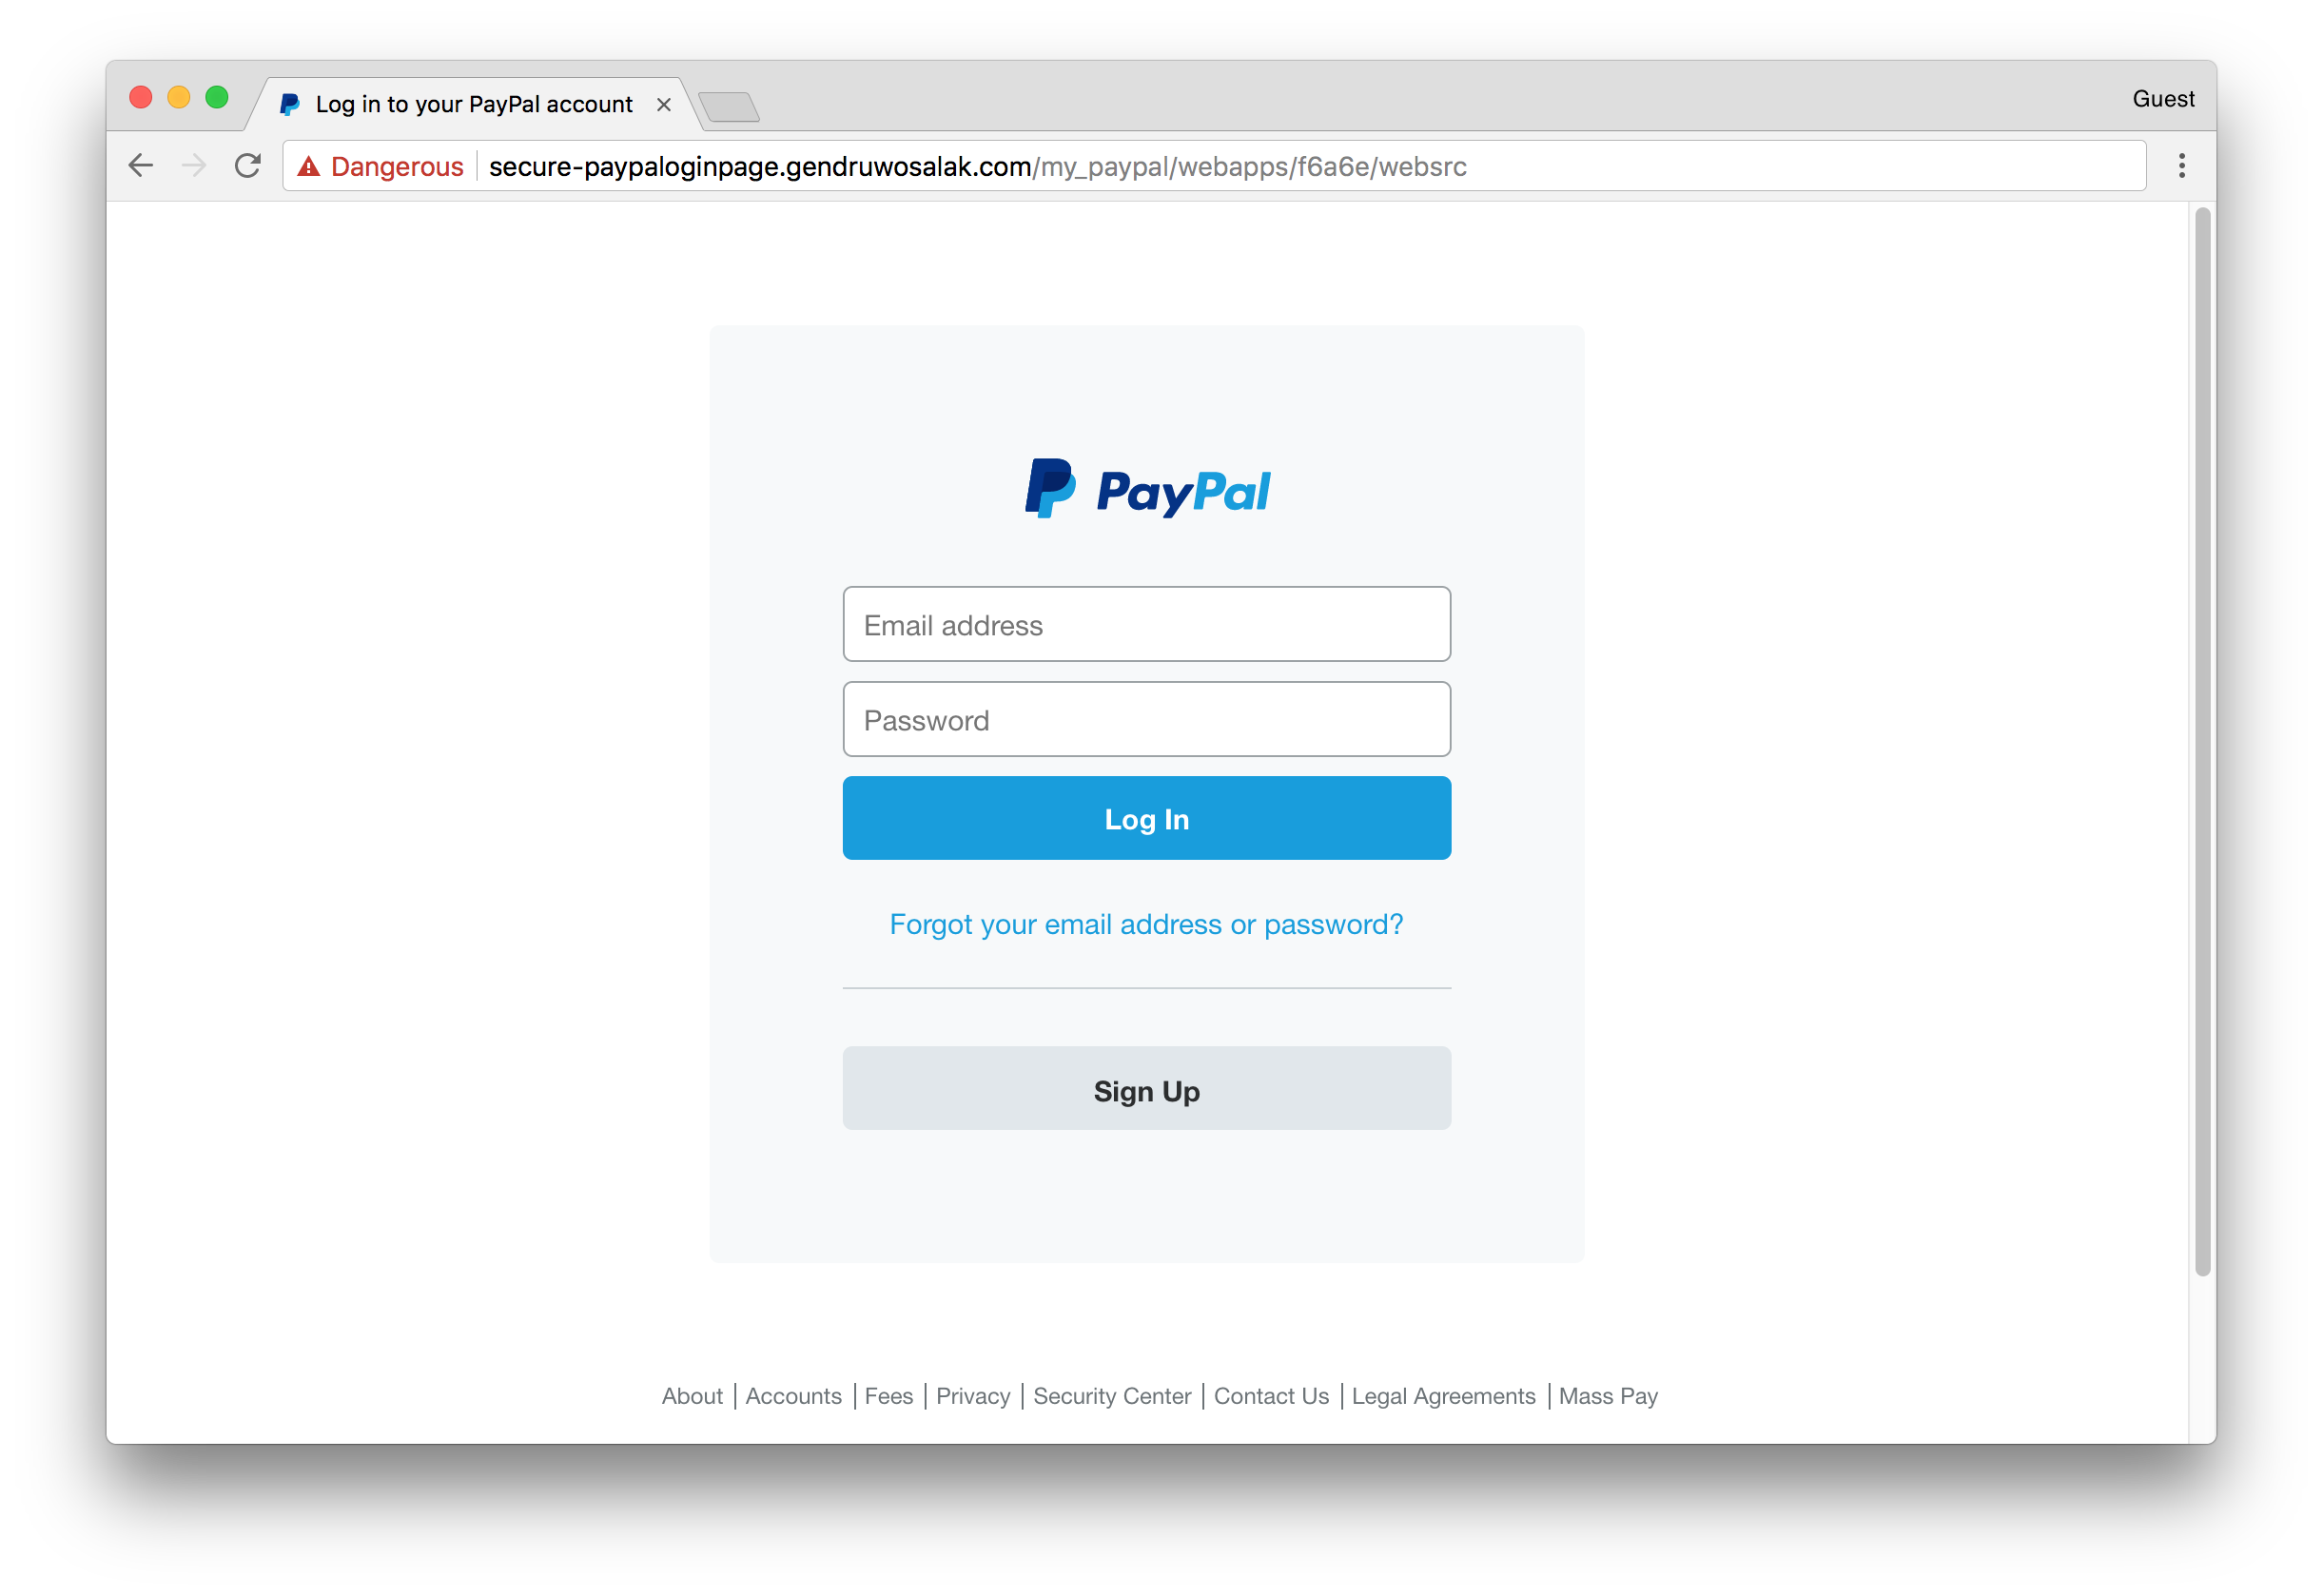
\includegraphics[width=0.7\linewidth]{rw/paypal-phishing-site}
	\caption{\label{fig:rw:phishingsite} Actual phishing websites targeting the facebook and paypal (online and accessible on 21.12.2017). The URLs contain ``fb'' (short for facebook) and keywords like ``secure'' ``paypal'' which contribute to falsely trusting the authenticity of the sites.\todo{propably split into two figures}}
\end{figure}

%%%%%%%%%%%%%%%%%%%%%%%%%%%%%%%%%%%%%%%%%
%%%%
%%%% p h i s h i n g
%%%%
%%%%%%%%%%%%%%%%%%%%%%%%%%%%%%%%%%%%%%%%%
\paragraph{Phishing / Social Engineering} 
% definition / high level description
Social engineering has become one of the biggest threats for a user's passwords with a growing number of incidents and fierce financial damage \cite{BKA2016Bundeslagebild}. Former criminal hacker Kevin D. Mitnick, who calls himself a social engineer, defines the term like this:
\begin{quotation}
	``Social Engineering uses influence and persuasion to deceive people
	by convincing them that the social engineer is someone he is not,
	or by manipulation. As a result, the social engineer is able to take
	advantage of people to obtain information with or without the use of
	technology.'' \cite[Frontmatter]{Mitnick2003ArtOfDeception}
\end{quotation}
Put simply, an attacker fools a victim into revealing certain kinds of information, including passwords. The most common social engineering attack on passwords is phishing, which typically involves two components: a fraudulent website that mimics another service and an email that lures the user onto this website \cite{Dhamija2006WhyPhishingWorks,Sheng2010WhoFallsForAPhish}. The email usually utilizes persuasive techniques like scaring  (``we noticed someone logged into your bank account and you need to reset your password'') time pressure (``you need to act \textit{now} to avoid further damage''). If the website looks just like the original (like the webpage in Figure \ref{fig:rw:phishingsite}), users might fall for it and enter their password to log in. In that case, it does not matter whether it is a strong, complex password or simply 12345 -- the attacker knows the username/password combination from that point on \cite{Tari2006ShoulderSurfingComparison}. If this tuple is used on other services, the attacker immediately gains access to them as well. 

% user perspective and mitigations
It is very challenging for users to validate the authenticity of a given webpage \cite{Dhamija2006WhyPhishingWorks, Fogg2001WhatMakesSitesCredible}. Usually, the URL is the best indicator, Dhamjia \etal among others argue that it is unrealistic to keep an eye on the URL at all times. Since the URL and padlock-icons are often ineffective, much research has been dedicated to help users in this validation and prevent phishing attacks. For example, Lin \etal found that domain highlighting in the URL bar only has a small effect on the effectiveness of phishing attacks, even after their participants were explicitly instructed to take not of the URL \cite{Lin2011DomainHighlighting}. Wu \etal showed that browser toolbars do not really help users, either \cite{Wu2006SecurityToolbars}. Dhamija \etal proposed a \textit{trusted path} between the user and the legitimate service \cite{Dhamija2005DynamicSecuritySkins}. In this system, users are supposed to verify the authenticity of a given website by comparing visual patterns in a trusted window and on the website. Together with Max-Emanuel Maurer and Alexander De Luca, I created a browser extension to visualize the usage of different types of SSL certificates across websites through the entire browser skin \cite{Maurer2011ShiningChrome}. We deployed it publicly and launched a feedback survey, which indicated that changing the browser skins is obtrusive enough to raise awareness and makes users more confident while browsing the Web. Until the recent change of platform APIs\footurl{https://blog.mozilla.org/addons/2017/11/20/extensions-in-firefox-58/}{21.12.2017} and resulting incompatibility problems, the extension named ``SSLPersonas'' had seen 47000 downloads, which is an indicator of both the necessity and the success of our solution. 

%% better solution: Browser prevents it by blocking phishing sites
However, optimally the browser would detect phishing websites and prevent that users visit them in the first place. Current versions of the major browsers try to do this and urge the user to leave the site, as is shown in Figure \ref{fig:rw:browser_warning}. This gives attackers only a short time-frame until the webpage has been classified as phishing, which takes around 4-8 hours according to a recent Webroot report \cite{Webroot2017PhishingReport}. Older sources report a bit longer lifespans between 20 hours\footurl{https://www.lightbluetouchpaper.org/2007/05/16/how-quickly-are-phishing-websites-taken-down/}{21.12.2017} and 54 hours\footurl{https://news.netcraft.com/archives/2004/08/14/life_span_of_a_phishing_site_averages_54_hours.html}{21.12.2017}. 

%%%%
%%%% Browser Warning deceptive website.
\begin{figure}
	\centering
	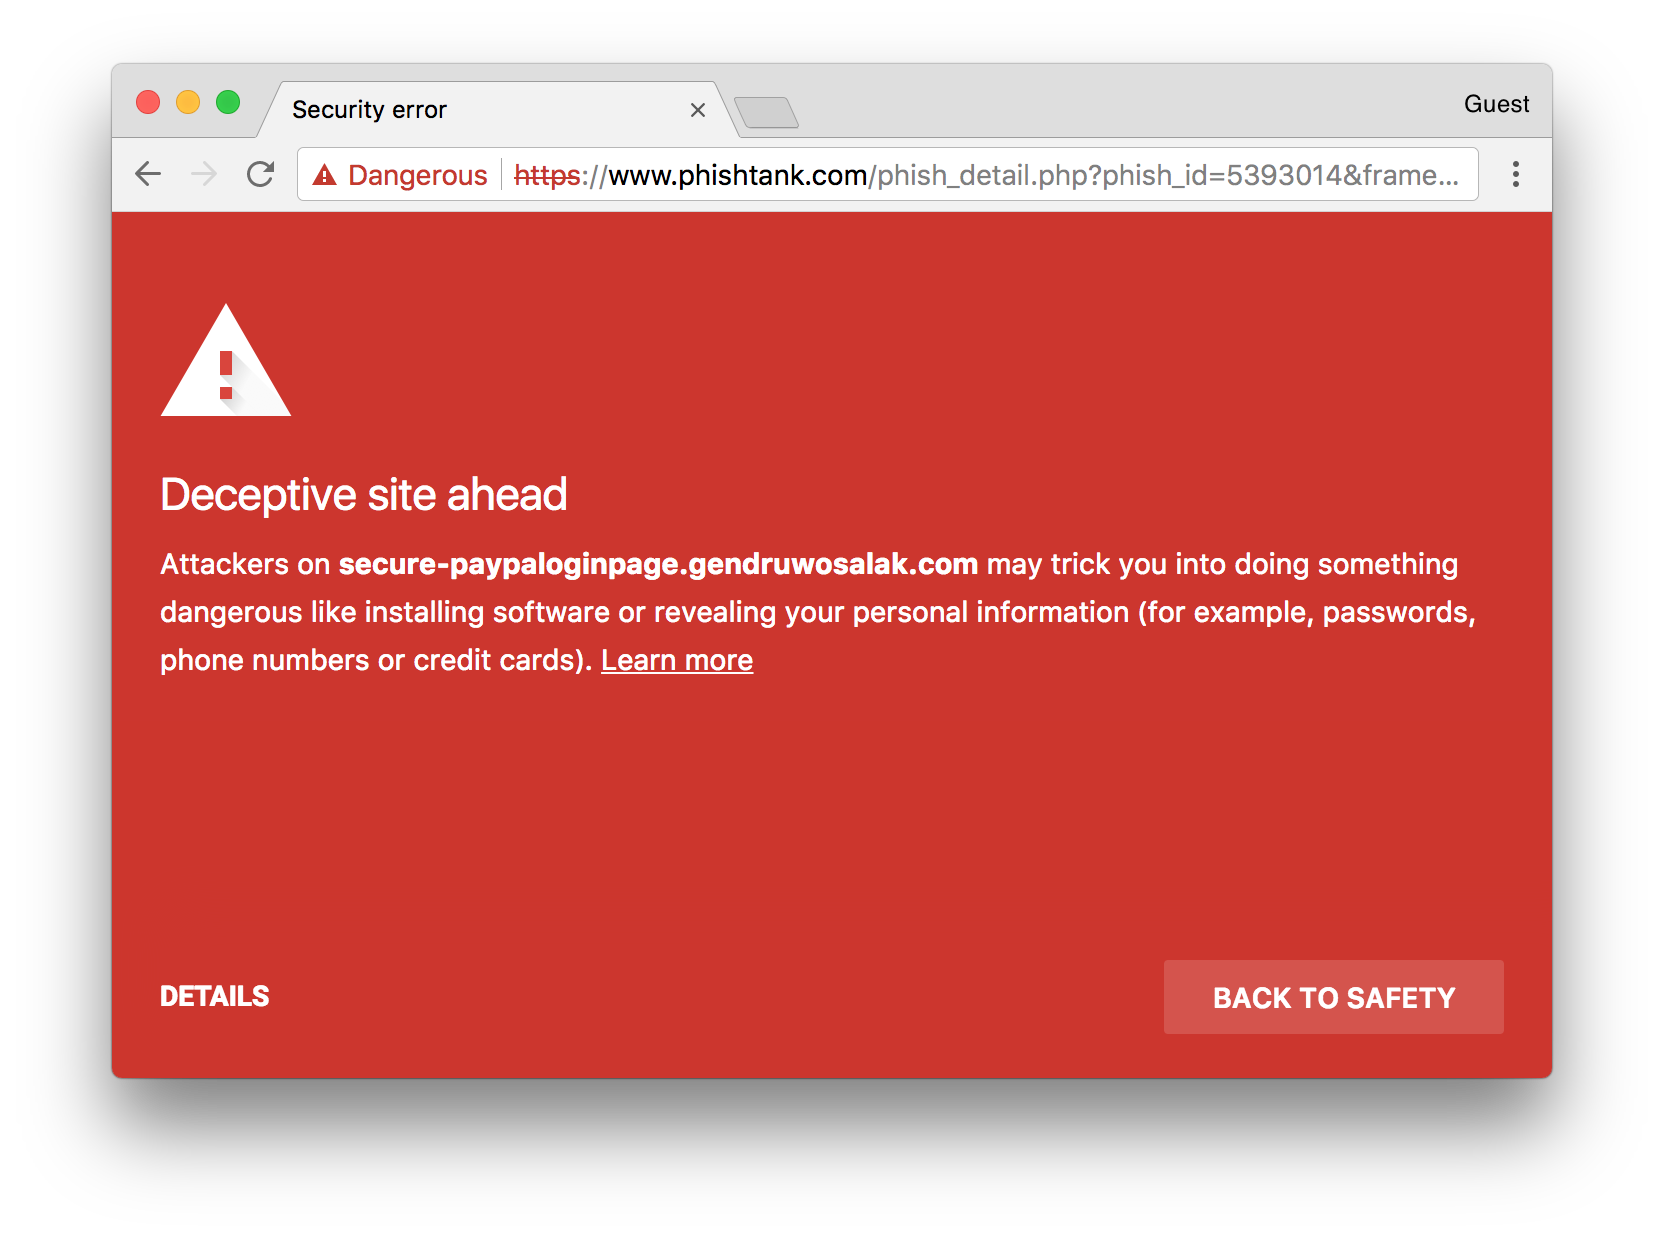
\includegraphics[width=0.8\linewidth]{rw/browser-warning-deceptive-site}
	\caption{\label{fig:rw:browser_warning}Chrome v63's warning on a phishing website. The user is urged to leave the site but still has the chance to visit it by clicking on ``Details''.}
\end{figure}

%%%%%%%%%%%%%%%%%%%%%%%%%%%%%%%%%%%%%%%%%
%%%%
%%%% m a l w a r e
%%%%
%%%%%%%%%%%%%%%%%%%%%%%%%%%%%%%%%%%%%%%%%
\paragraph{Malware and Eavesdropping} 
% attack description and types: keylogger.
Secretly stealing plain-text passwords is also possible by infiltrating the user's system with \textit{malware}, which is a term for \textit{mal}icious soft\textit{ware} \cite{Bayer2009CurrentMalware}. One of most common attacks is to install a keylogger that sends all keystrokes to the attacker. For the most part, this either happens as a ``drive-by-download'' when the user visits an infected website or by opening a malicious email attachment \cite{BKA2016Bundeslagebild}. In the former scenario, the sole line of defense lies with the service provider who needs to make sure their website is not infected.
% user perspective
Wash identified that users are aware of this kind of threat, but their mental model of malware is sub-par \cite{Wash2010FolkModels}. Hence, the countermeasures taken by the users are often insufficient. As with the phishing scenario, a strong password is incapable of preventing a malware attack. Ideally, users use an anti-virus solution, keep their software updated at all times and refrain from opening suspicious email attachments. 

% man in the middle attakcs
Moreover, user credentials can be intercepted in transit, e.g. after the user submits them through a web form. These so called man-in-the-middle attacks are tough to carry out, but strong passwords do not prevent them either. 
% solutions
One of the typical solutions to minimize the risk is encrypting the traffic with a secure protocol like SSL/TLS \cite[p. 853ff.]{Tanenbaum2011ComputerNetworks}, which is based on a public/private key infrastructure. This makes it harder for an adversary to act as the man in the middle, because they usually do not possess the necessary private key of either party. Attackers must tamper with the certificates which usually causes browsers show a warning \cite{Maurer2011ShiningChrome}. 
% user perspective 
Users, however, do not necessarily understand such warnings, because their understanding of the technical details is low \cite{Herley2009SoLongThanksExternalities, Whitten1999WhyJohnnyCantEncrypt}. Consequently, the HCI community has invested much effort to convey the essential messages in a clear and actionable way \cite{Felt2015ImprovingSSLWarnings, Felt2014ChromeSSL,  Maurer2011ShiningChrome, Sotirakopoulos2011ReplicationSSLWarnings, Sunshine2009CryingWolf}.

%Keyloggers, eavesdropped communication (e.g. via Man in the Middle Attacks)

%%%%%%%%%%%%%%%%%%%%%%%%%%%%%%%%%%%%%%%%%
%%%%
%%%% o b s e r v a t i o n 
%%%%
%%%%%%%%%%%%%%%%%%%%%%%%%%%%%%%%%%%%%%%%%
\paragraph{Observation} 
%what's the problem? how does the attack work? what are countermeasures from a technical side? what are countermeasures for the users? do strong passwords help? skill level required by the attacker?
To obtain the password of a specific user, one can also simply watch them enter it and figure out what the password was. This attack is typically referred to as ``shoulder surfing'' because the person who watches figuratively ``surfs'' on the user's ``shoulder'' to look at their screen \cite{Tari2006ShoulderSurfingComparison}. Shoulder surfing is relatively easy and does not require technical sophistication. But, although friends and family can carry out such an attack, it is safe to say that it is more problematic in public spaces where unknown bystanders are present. Typical interactions that take place in such environments can be found with PIN entry, e.g. on an ATM, or entering any kind of password on a mobile device, e.g. on a bus in close vicinity to other people. 
% new system as countermeasure: De Luca / ColorPIN
De Luca \etal dedicated some research to both scenarios. For instance, they investigated contextual factors during ATM usage and the design space for alternative ATM authentication mechanisms \cite{DeLuca2010UnderstandingATMSecurity}. They developed the ColorPIN scheme \cite{DeLuca2010ColorPIN}: Additionally to the number sequence, the user needs to memorize a \textit{color} sequence, e.g. 1 (\textbf{black}) - 2 (\textbf{red}) - 3 (\textbf{white}) - 4 (\textbf{black}). \todo{it would be nice if the text were in that color too} Entering the PIN is done through indirect input: Instead of prompting the user to enter the digits directly on the keypad, the system displays digits accompanied by three distinct letters in black, red, and white underneath. The keyboard through which the ColorPIN is entered, shows each letter three times -- once in each color. To enter the ColorPIN, the user needs to first identify the correct digit (e.g. ``1''), and then type the corresponding letter in the right color (e.g. a black ``Q''). After each entered character, the letter assignment is randomized again. All of this makes it challenging for a shoulder surfer to quickly observe and learn the user's PIN by overwhelming their short-term memory \cite{Dunphy2010CloserLookGraphical}.

% it's mostly PINs and graphical passwords rather than alphanumeric ones
Moreover, long alphanumeric passwords are a seldom research topic with regard to shoulder surfing. Shaub \etal looked into the effect of different designs of virtual keyboards on shoulder surfing susceptibility \cite{Schaub2012PasswordShoulderSurfing}. Somewhat unsurprisingly, they found that keyboards with more cumbersome access to special characters are less prone to shoulder surfing. We can see in the ColorPIN example, PINs and graphical passwords are more perceived to be under attack. Users usually enter graphical passwords more slowly \cite{Tari2006ShoulderSurfingComparison, Wiedenbeck2006ConvexHull, Renaud2009VisualSnakeOil}, which on the one hand gives an attacker more time to observe, but on the other hand burdens the short-term memory a bit more. Also, some visual authentication mechanisms require more screen real estate than a username/password form and entry is often not masked \cite{Biddle2009GraphicalFirstTwelveYears}. Still, there is not a lot of evidence that observation is a severe threat in the real world, other than for ATM PINs and any kind of credentials of people of public interest. Herley and Pieters point out that the attack is not scalable via algorithms like offline guessing \cite{Herley2015Counterfactuals}. Hence, Maguire and Renaud come to the conclusion that ``shoulder-surfing may well be a non-issue in authentication design'' \cite{Maguire2012YouOnlyLiveTwice}. 
% what about shoulder surfing on the web?
In the same On the web, observation is rarely a major concern. 



not only passwords but anything that you do on a computer can be shoulder surfed, e.g. text messages \cite{Eiband2016MyScrawl}.


typically graphical password schemes are more concerned with this attack, because the screen real estate needed to display and enter them is usually higher.  \cite{Tari2006ShoulderSurfingComparison} 
in general the attack is prevalent with authentication in public spaces, e.g. atms or on mobile devices. \cite{DeLuca2013BackOfDevice} \cite{Roth2004PINShoulderSurfing} PINs are easier to observe than pws because they are shorter and only numerical -- realistically for atms, where a two factor system is in place an attacker first needs to observe the pin and then steal the hardware token (magnetic strip cards)

On screen keyboards: De Luca \etal displayed multiple cursors on screen that acted as distractors. For users it was easy to recognize the actual mouse cursor 
\cite{DeLuca2013FakeCursors}


Shoulder surfing, passwords on post-its at the office. that's why passwords are masked in the browser (with an asterisk per character), but the benefit has recently been questioned \cite{Sasse2016DebunkingMyths}. 



%%%%%%%%%%%%%%%%%%%%%%%%%%%%%%%%%%%%%%%%%
%%%%
%%%% o t h e r    a t t a c k s
%%%%
%%%%%%%%%%%%%%%%%%%%%%%%%%%%%%%%%%%%%%%%%
\paragraph{Other attacks} 
Apart from the attacks described above, there are other approaches that should not go unmentioned. First, people in one's own social circle, e.g. friends and family, have much personal information and often physical access to devices and passwords written onto post-it notes. Although the intent is often not purely malicious, it can be easy for these people to have an informed guess of a user's credentials. Flechais \etal use the term ``spouse attack'' to describe this kind of threat \cite{Flechais2013SaudiArabiaTrust}, Dunphy \etal call it a . Ur \etal found that users underestimate its likelihood \cite{Ur2016PerceptionsPassword}. A strong, complex password that is only memorable to the legitimate user might help in that scenario. Weirich and Sasse, however, argue that such a strategy could make the user appear ``paranoid'' \cite{Weirich2001PrettyGoodPersuasion} and Flechais \etal see it as an important sign of trust \cite{Flechais2005DivideConquerTrust, Flechais2013SaudiArabiaTrust}. 
 
%%%% unintentional disclosure
Finally, some credentials are shared unintentionally on the web. Software developers who share open source code on the web are prone to this issue. Recently, the node package manager (npm) platform realized that many of its users published their passwords with the packages\footurl{http://blog.npmjs.org/post/161515829950/credentials-resets}{22.12.2017}. An adversary could simply crawl public repositories on GitHub and collect the passwords in plain text. The npmjs.org operators had to invalidate the credentials to secure the accounts. One solution that reduces the severity of credential loss is using multi-factor authentication (cf. Section \ref{sec:rw:shared_auth_tokens}).


%%%% 
%%%% TABLE: Attacks and Countermeasures
% Table generated by Excel2LaTeX from sheet 'attacks-mitigations'
\begin{table}[htbp]
  \centering
  \caption{\label{table:rw:attacks_countermeasures}Threats on passwords and potential countermeasures for users and service providers (SP). Other stakeholders are left out of this analysis.}
    \begin{tabular}{rll}
    \multicolumn{1}{l}{\textbf{Threat}} & \textbf{Countermeasures} & \textbf{Responsible} \\
    \hline
    \multicolumn{1}{l}{\textbf{Online Attack}} & Throttling & SP \\
          & Anomaly detection & SP \\
          & Set-up Multi-factor authentication & SP \\
          & Moderately complex password & User \\
          & Enable Multi-factor authentication & User \\
    \multicolumn{1}{l}{\textbf{Offline attack}} 
        	& Slow hash algorithm & SP \\
			& Secure database design & SP \\
			& Security audits, fix vulnerabilities & SP \\
		    & Complex, strong password & User \\

    \multicolumn{1}{l}{\textbf{Phishing}} & Education and Warnings & SP \\
    & Unique passwords & User \\
          & Check security indicators & User \\
          & Utilize spam filter & User \\
          & Vigilance regarding emails & User \\
    \multicolumn{1}{l}{\textbf{Malware}} & Anti-Virus software & User \\
          & Caution on the web & User \\
    \multicolumn{1}{l}{\textbf{Observation}} & Password masking & SP \\
    	& Awareness of surroundings & User \\
    \end{tabular}%
\end{table}%
\todo{make this more convincing}
%%%%
%%%%

%TODO Florêncio \etal proposed a classification for attacks \cite{Florencio2014PasswordPortfoliosFiniteUser}. Class 1-3

%TODO what is an attack ``vector''? attack steps from start to success. \ar
%Sometimes combinations of attacks (vector)

The main objective of this thesis is combating online and offline attacks, i.e. for algorithmic attacks, where password coping strategies really make a difference. A panacea for all kinds of threats, each of which has warranted multiple PhD theses, is probably impossible to find. 



%%%%%%%%%%%%%%%%%%%%%%%%%%%%%%%%%%%%%%%%%
%%%%
%%%% w h a t    i s    p a s s w o r d    s t r e n g t h
%%%%
%%%%%%%%%%%%%%%%%%%%%%%%%%%%%%%%%%%%%%%%%
\section{What is Password Strength? - Metrics and Statistics}\label{sec:rw:pw_strength_metrics}
Bishop and Klein said in 1995: ``A good password is one that is easily remembered, yet difficult to guess.'' \cite[p. 231]{Bishop1995ProactivePasswordChecking}. The second part of this statement describes password \textit{strength} on a high level. But there are problems if we try to objectively measure the ``difficulty to guess'' a password: is it difficult for an attacker with nearly unlimited resources, or only for an attacker that can only attempt once a day due to lock-out mechanisms? The question is highly context dependent and there is unfortunately no single true answer. 

How to attack passwords
- here the most important paper is:
Cracking techniques must be used in parallel to get the complete picture of password guessability \cite{Ur2015MeasuringRealWorldAccuracies} -- mention tools like HashCat/oclHashcat, John The Ripper 

give some real world examples how passwords are attacked online and how they have been attacked offline. 


Lately the community reached widespread consensus that the realistic strength of password can be defined as \textit{the number of attempts that an attacker would need in order to guess it} \cite{Dellamico2015MonteCarlo}

 

Don't forget: Password strength is dynamic! New leaks can render strong passwords very weak. Yang \etal state: ``If a strategy is widely used, then attackers may develop strategy-specific methods which can efficiently guess the passwords.'' for example: if passphrases do become commonplace, attackers will optimize their attack strategy. in the end, the number of leaked passwords will continue to grow so it is tedious to ``outrun'' hackers by resetting passwords etc.

Bonneau looked at leaked passwords and tried to attack them in different ways to find patterns in user behavior that could be leveraged in real-world attacks \cite{Bonneau2012ScienceOfGuessing}. Fundamentally, the attacks were based on different dictionaries. He found that the success rates of attacks strongly depend on the dictionary that is used for it. Under the assumption that entropy is a viable strength proxy, he concluded that 10 bits of entropy are probably enough to defend against online attacks, respectively 20 bits for offline attacks. 

\cite{Peisert2013PriciplesAuthentication,Bonneau2012ScienceOfGuessing,Scott1995GDMS,Dellamico2015MonteCarlo,Ur2015MeasuringRealWorldAccuracies,Egelman2015SeBIS,Conklin2004PWAuthenticationSystemPerspective,Schmidt2013Pitfalls,Kelley2012GuessAgain,Mazurek2013Measuring,Weir2010MetricsPolicies}

	\subsection{Entropy vs. Guesswork}
	
	Other definitions: ``The strength of a password should represent the amount of effort an adversary must employ to break the password'' \cite{Carnavalet2014AnalyzingPWStrengthMeters}.
	
	William Burr regrets NIST policy (see footnote \ref{foot:burr_regrets})	
	
	
	
	Entropy (Shannon) -- degree of randomness. often too focused on characters and doesn't address human password selection, which is far more predictable 
	(effective vs. theoretical password space)
	
	@@TODO tell the story of all the attacks -- Kelley, Weir, Bonneau, Melicher, Johnson, Ur etc. Password Guessability Service etc. 
	
	Leaked password dictionaries: Most commonly: RockYou (gamer site), MySpace, LinkedIn, Gawker, Yahoo!
	Mark Burnett  \cite{Burnett2005PerfectPasswords} 
	
	Tell the history of how guesswork was modeled. Starts out with \cite{Weir2010MetricsPolicies}, then \cite{Kelley20012GuessAgain} and \cite{Bonneau2012ScienceOfGuessing}. 
	
	Weir et al established a guessing method where the most probable passwords are tried first (PCFG) and measure how many passwords can be cracked until a cut-off threshold, and this resulting metric is more valid than entropy \cite{Weir2010MetricsPolicies}
	
	NIST entropy was THE measure for password strength until the Weir paper and shortly afterwards. \cite{Komanduri2011OfPasswordsAndPeople} is probably the last CMU paper that uses entropy as strength metric (and is proud of it).
	
	Entropy is relative to / dependent on a given set of passwords. 
	
	Passfault can crack passwords and is open source \cite{Paiva2017Passfault}
	
	Neural networks perform really well to crack passwords if you configure them correctly and you can even do this in the browser, but it's not super trivial \cite{Melicher2016NeuralNetworks}
	
	\subsection{Beta-guess-rate}
	$\lambda_{\beta}$
	quasi: how likely is it to find the top $\beta$ passwords in a given dataset?
	see bonneau, and also used in \cite{Yang2016MnemonicSentenceBased}
	brostoff and sasse  proposed 10 as a threshold for rate-limiting (before account is locked and password invalidated until reset) \cite{Brostoff2003TenStrikes}
	
	
	
	
	\subsection{Strength Proxies: The zxcvbn Approach}
Daniel Wheeler presented an approach towards password strength estimation by looking at a conservative expected guess attempt number \cite{Wheeler2016zxcvbn}. The idea is to utilize pattern matching against dictionaries and leaked password corpora and then calculate the minimum rank over a series of frequency ranked lists. In other words, the approach is heuristic instead of probabilistic, because the ranking is based on searching through the patterns and ranking them not only based on their likelihoods, but other factors like keyboard sequences. The implementation of the algorithm is called zxcvbn\footnote{The name zxcvbn originates from the bottom row on a QWERTY keyboard. Many users mistakenly consider this approach secure because the resulting password looks fairly random.}. Wheeler showed that in an online attack scenario \cite{Florencio2014AdministratorsGuide} the algorithm estimates the number of guesses accurately within an order of magnitude of 2 -- consistently better than NIST guidelines to date and KeePass strength estimators. That is, utilizing 100,000 tokens stored within a 1.5 Megabyte file zxcvbn conservatively estimates the number of guesses required to crack a password. Beyond the online-attack threshold, the results are mixed, but we can observe that adding more tokens to the dictionary improves accuracy even more. The great benefit of using this method is its speed and size that make it a lightweight tool that is prepared for widespread adoption, to relieve users from ``LUDS'' policies (lowercase, uppercase, digits, symbols). We can conclude that zxcvbn is a reasonable tool when we collect meta statistics about passwords, e.g. in studies where it is ethically questionable to collect plain text passwords \cite{Seitz2016SuggestionsDecoy}. Wheeler also points out that at this point there is no study comparing the effects the different estimators have on user behavior. 

papers that used or mentioned zxcvbn:
\cite{Komanduri2014Telepathwords}
\cite{Wang2016fuzzyPWM}
\cite{Ur2017DataDrivenPWMeter}
\cite{Yang2016MnemonicSentenceBased}
\cite{Gross2016CognitiveDepletion}

Weaknesses \cite{DeCarnedeCarnavalet2015PasswordMeters}: only english dictionary words, fixed dictionary with the constraints of being transfered to the client, so some passphrases are considered strong while they are not really super great, e.g. ``dolce\&gabana''
not true anymore but in the paper: reversed passwords are not recognized (Wheeler updated this). 


\section{What is a ``Bad'' Password?}
This question is flawed, and thus cannot be answered without context. The word ``bad'' is judgmental and depends on whom is asked. A security expert might call a password ``bad'' if it only contains lowercase letters, but a regular mainstream user might call it ``bad'' because they cannot type it quickly or can't remember it well. 

Bishop and Klein said in 1995: ``A good password is one that is easily remembered, yet difficult to guess.'' \cite[p. 231]{Bishop1995ProactivePasswordChecking}

Let's look at 

types of attacks: phishing, online (rainbow), offline, targeted online. \cite{ZhangKennedy2016RevisitingPasswordRules}. 

When does password strength really help? 

This paragraph from Herley and Van Oorschot says it all \cite{Herley2012PersistenceOfPasswords}:
``Fifth, when are off-line attacks a threat? While dependent on implementation, access to salted hashed pass- words requires attacker effort; long gone are the days when password hash files were by default world read- able. A disgruntled ex-sysadmin who steals hashed pass- words is the often-conjectured foe in this attack; yet, if un-trusted individuals have had unfettered unaudited access to the authentication server, a site’s problems go well beyond password strength. Sixth, are there ways to protect against off-line attacks besides password strength? Mandating password changes once hashes leak might be better than strong policies at all times. Only if a leak goes unnoticed (and a password change isn’t forced) does strength potentially help. Of course, reliably detecting leaks or break-ins it- self remains difficult. Finally, how much strength is required to protect against off-line attacks? The bar is clearly much higher than for online attacks (assuming lockout or rate-limiting policies in place), but at what strength are attacks effectively addressed? More strength is always better for security,'' 

discuss online and offline attacks
\cite{Wang2016fuzzyPWM} has an overview/comparison
\cite{Florencio2014AdministratorsGuide} shows models
\cite{Florencio2014PasswordPortfoliosFiniteUser} has math

A problem about only taking ``online'' attacks into account is that they do allow denial of service attacks, for example if there's lockout policy in place that invalidates passwords after 10 failed login attempts, an attacker would only need to take a list of email addresses (readily available on the internet) and run 10 or more guesses per user and lock all of them out at once. 



We shouldn't call it good or bad. A less judgmental terminology is ``strong'' and ``weak'' because this doesn't include opinions. 

A ``strong'' password is one that cannot be guessed easily by a human or a machine, regardless of the level of information they have about the owner of the password. 


The idea behind a PCFG based policy is to reject passwords that are too ``probable''. 

Characteristics of weak passwords \cite{Burnett2005PerfectPasswords}
\begin{enumerate}
	\item Are used by many users
	\item Can be found through an internet search
	\item Are short (6 characters or less)
	\item Have leaked
	\item Are written down where anyone can access them
\end{enumerate}

But there are other, non-technical qualities of passwords that are usually not covered by the weak-strong spectrum. 

When is a password \textbf{``Appropriate''}? This largely depends on the usage context. \cite{Gaw2005ReuseRecycle, Haque2014Hierarchy}
Florencio \etal argue that it is absolutely fine to choose a weak password for ``don't-care'' accounts \cite{Florencio2014}.

Requirements from a user perspective: memorable and easy/fast to type on all devices.

this creates tensions that are discussed in detail in Chapter \ref{chap:rw:user_perspective}.


\section{Authentication beyond Passwords}\label{sec:rw:authentication_without_pws}
The benefits and drawbacks of using passwords have been studied extensively. Some drawbacks already become apparent when we recall Ali Baba's story: Ali Baba overhears the thieves saying the magic words and can immediately authenticate with them (a big security issue). He also told the ``password'' to his brother, but he fails to recall it (the biggest usability issue).

Table \ref{table:rw:benefits_drawbacks_pws} shows a high-level summary of the benefits and drawbacks that come along with password-based authentication. We can observe that the drawbacks constitute important constraints and it is natural to try to remove such limitations by considering alternatives. This section briefly covers the most notable approaches to authenticate users without alphanumerical passwords.

\begin{table}
	\begin{tabular}{|l|l|l|}
		Benefits | Drawbacks 
	\end{tabular}
	\caption{\label{table:rw:benefits_drawbacks_pws}Benefits and Drawbacks of passwords for different stakeholders}
\end{table}
%benefits: easy to implement, users know how they work, concept is easy to learn, can be shared, can be replaced when they are compromised, can be revoked by the sys admin, quick to enter, work without a user name (WiFi) so it's easy to scale. 
%drawbacks: users have to cope with many passwords, so they use risky strategies \ref{sec:rw:how-users-cope}, it's difficult to manually create a password that is both usable and secure (good enough to protect against offline attacks)




% das passt nicht unbedingt hier rein, ist aber sehr wichtig. 
Bonneau et al. argue \cite{Bonneau2015ImperfectAuthentication} that passwords are an imperfect technology that is difficult to replace. One, industry has found ways to work around the many drawbacks and can compensate breaches to a large part. Second, alternatives to passwords are often privacy invasive. For example, identity providers like Google or Facebook often collect large amounts of personal data on the users. Third, Bonneau et al. point out that empirical evidence from practice often contradicts results produced by academic research. They advocate that researchers rethink their model of users, who often behave too predictably and whose behaviors one should not try to change. Instead, academia could tackle new approaches that would be dangerous to the success of businesses and thus are seldom tried out. 

% noch mehr Zusammenfassung für später:
The authors point out how user models assumed by researchers often do not apply in reality, for instance, their behavior is anything but random: Users pick from a limited set of passwords that is far smaller than random passwords. Just as \cite{Florencio2014PasswordPortfoliosFiniteUser}, the paper strongly discourages focusing on offline attack scenarios and suggests that users should at most try and protect themselves against online attack scenarios. Consequently, the lessons from the past about attempts to improve password strength through changing user behavior are questionable in the authors' eyes. Even more so, because other attacks (phishing, malware, eavesdropping, stealing from servers or identity tokens) are not fended off at all by stronger passwords. Online attacks can drastically be mitigate by rate-limiting and contextual information (e.g. geolocation). Yet, the authors see that not all sites employ these methods, ``probably to avoid denial of service''. Users also often receive too much advice from security experts that is often contradictory and in extreme cases boiled down to ``Pick something you cannot remember and do not write it down''. 

Bonneau et al. answer the question whether we still need passwords with a differentiated ``yes'': \textit{Passwords appear to be a Pareto equilibrium\footnote{\todo{add definition of this here. It's about game theory.}}}. Also the learning curves for password authentication at a new service is virtually non-existent. However, as many researchers in the community, the authors see the feasibility of multi-factor authentication in progressive or continual ways as the most promising future. The challenges for privacy and usability we find in these approaches are mostly ill-defined or not validated. The user experience of such systems may improve while the drawbacks come at a high price that the users may not understand at all. 

	\subsection{Graphical Passwords \& Visual Authentication Methods}
Graphical passwords can work for children and adults \cite{Imran2015PWsAdultsChildren}

, Ema's work, \cite{Renaud2009VisualSnakeOil} 

	\subsection{Biometrics}
	
	\cite{Jakobsson2014HowToWearYourPW,DeLuca2012TouchMeOnce,Peisert2013PriciplesAuthentication,Rybnicek2014RoadmapContinuousAuth}
	

	fingerprint omnipresent 
	retinal scan
	face recognition (iPhone X)
	
	
	Anecdote to show that it is a bad idea\footnote{\url{https://www.theguardian.com/world/2017/nov/08/qatar-airways-plane-forced-to-land-after-wife-discovers-husbands-affair-midflight}, \access{08.11.2017}}
	
	\subsection{Multimodal and Implicit Authentication}
	
	actually the technical report gives some insights about this \cite{Stockinger2011ImplicitAuthentication}, so that will inspire a bit.
	also look into the USEC folder in the office, the papers and annotations are in there.
	
		it's interesting that the most cited CHI paper of the last 5 years is about implicit authentication \cite{DeLuca2012TouchMeOnce}
		
		\cite{Roalter2013SmartphoneProxy}
	
	Machine learning. Accuracy / Recall / Error rate / True Positve / False Positives etc. -- based on \textbf{probability} and not on \textbf{certainty}. To account for the lack of certainty, in all current state-of-the-art mechanisms passwords serve as fallback authentication. So, while it reduces the number of password entries and so speeds up interactions in many cases, these schemes cannot fully replace passwords. What is worse is that the rare interaction often tempts users to choose a very memorable secret, which in most cases is weaker than a password that is entered on a regular basis. So an attacker that is successfully denied access to a system protected by multimodal authentication will always have the opportunity to authenticate with a password -- the system needs to assume a false negative and offer the fallback authentication scheme. In this scenario, while the primary authentication is more usable and very secure, the entire system's security is lowered by its fallback scheme. This fact is often played down and neglected in the marketing of new multimodal authentication. 
	
	Take away: implicit authentication cannot replace explicit authentication, but it can make an existing scheme more secure. Fallback schemes tend to lower system security. 
	

in a study setting, giving users power over their authentication scheme worked well, but it might not in real-world settings \cite{Forget2015CYOA}
	
	\subsection{Shared Authentication and Hardware Tokens}\label{sec:rw:shared_auth_tokens}
Single Sign-On (SSO). 
Identity Providers, 
SecureID or ``Gnubby'' (see Google)
Two-Factor Authentication / 2-step --> hints to 2-step in ``Some UNIX systems have instituted what is called an "external security code" that must be typed when dialing into the system, but before logging in. If this code is changed periodically, then someone with an old password will likely be prevented from using it.'' \cite{Morris1979PasswordSecurity}


If authentication mechanisms were a tournament, users would prefer OAuth and QR-Codes to authenticate, but in the real world, this isn't the case \cite{Ruoti2015AuthenticationMelee}

Reference Models:
\cite{Egelman2013ProfilePassword,Sun2010BillionKeys}

\begin{itemize}
\item \textbf{OAuth} Twitter, Google
\item \textbf{OpenID} Google, PayPal
\item \textbf{Facebook Connect} 
\end{itemize}
Problems: 
Successful identity providers such as Facebook take a central role as the ``sole identity provider, which does little for privacy'' \cite{Bonneau2015ImperfectAuthentication}.


\textbf{Privacy} The biggest players for shared authentication are Facebook, Google, and Twitter. However, it is exactly these three companies for which users raise the most privacy concerns. On the one hand, users trust the companies because they know how much data they store and manage, and only few breaches are known. On the other hand, users are doubtful that their credentials will be in safe hands and not shared with third parties (users lack the understanding of how shared authentication works internally and cannot separate privacy and security). 

\textbf{Single Point of Failure} Embracing the opportunities of shared authentication, users integrate it into their password management / coping strategies \ref{sec:rw:how-users-cope}. 

	
\subsubsection{One Time Passwords}

OTP also have the possibility to replace a password that you have to memorize, but there are disadvantages as well. 
illustrate the workflow from Slack.

Authentication Melee paper has some intel on one-time passwords: \cite{Ruoti2015AuthenticationMelee}


\section{Passwords are Here to Stay}
no solution fully replaces them

most approaches that are seen as more usable are often based on probability rather than certainty (TPR / FPR / EER). fallback to passwords probable even for other authentication schemes. everything else is often less usable than passwords. 

maybe discuss this at the end of the thesis: passwords are cool, and we can continue to use them because they are so easy to replace in case of a breach. 

An approach that is currently not undertaken in internal security audits is the following: there are password leaks once a month (see data breach reports). the security team could take the passwords (if they are hashed - crack them first) and invalidate all matching passwords in their own password database. Of course, they need to inform their users. I could sketch a flowchart what this should look like. This would allow reusing passwords more securely without shifting much responsibility to the users. 

``We argue that it is time to admit that passwords will be with us for some time, and moreover, that in many instances they are the best-fit among currently known solutions.'' \cite{Herley2012PersistenceOfPasswords} 

The Herley and Van Oorschot paper really has lots of good quotes and thoughts for this
We need a more systematic research approach about passwords to make users' lives easier and we shouldn't try to find a single scheme that replaces them (impossible) but a more triangulated approach \cite{Herley2012PersistenceOfPasswords}


\cite{Kirlappos2012SecurityEducation,Loutfi2015PasswordsOtherSideOfTheFence,DeAngeli2005PictureThousandWords,Florencio2013WhereDoAllTheAttacksGo,Herley2008ProfitlessEndeavor,Sasse2015,Dittrich2009,Herley2009SoLongThanksExternalities,Vantaggiato2015WeStillNeedPasswords,Florencio2010WhereDoPoliciesComeFrom,Schrittwieser2013,Bonneau2015ImperfectAuthentication,Cyber2014,Florencio2007DoStrongWebPasswords,Sasse2005UsableSecurityPosition,Aebischer2017PicoInTheWild,Forget2007HelpingUsers,Herley2009IfWereSoSmart,Acar2016NotYourDeveloper,Sasse2016,Renaud2009VisualSnakeOil}



\chapter[Passwords -- A User Perspective]{Passwords -- \\
	A User Perspective}\label{chap:rw:user_perspective}
%lingo: arduous

``but his thoughts were so full of the great riches he should possess, that he could not think of the word to make it open, but instead of `Sesame,' said, `Open, Barley!' and was much amazed to find that the door remained fast shut. He named several sorts of grain, but still the door would not open, and the more he endeavoured to remember the word `Simsim,' the more his memory was confounded, and he had as much forgotten it as if he had never heard it mentioned.'' (Kasim's predicament in \textit{Ali Baba and the Forty Thieves}) \todo{this could be the opening of the chapter / fancychapter}

Morris and Thompson were already concerned with user behavior regarding passwords in 1979 \cite{Morris1979PasswordSecurity}. They identified that users choose predictable passwords and that this can be leveraged for attacks. So, they suggested enforcing a certain minimum password length (six characters). At the time, the users were mostly professionals that received training to operate computers and could thus also have been trained to pick less predictable passwords \cite{Maguire2012YouOnlyLiveTwice}. But as computers were introduced to a larger audience, more people were exposed to password authentication. Naturally, this also induced a growing number of attacks, and it is increasingly difficult for users to defend themselves against them (see. Section \ref{sec:rw:attack_vectors}). Nowadays, password policies are in place that require not only a minimum of eight characters, but also mandate mixed-case letters, digits and special symbols to start with. The HCI community noticed the users' struggle in the 1990s and that we can -- and should -- design authentication systems with usability in mind. Perhaps, one of the breaking points where a new school of thought turned up in the literature was a paper by Adams and Sasse in 1999 \cite{Adams1999UsersEnemy}. The central and novel theme in there was a shift from \textit{fixing} the user to \textit{acknowledging} user behavior and designing for it. The paper managed to see over 1500 citations as of writing this.

This chapter looks at the literature that mostly came after this seminal work. It discusses the users' problems, solutions, feelings, and opinions about using passwords. An essential goal is to give the reader an empathetic perspective and provide background information to understand why it seems hard to come up with viable solutions to make users' lives less frustrating. To get there, we first take a brief look at conducting user research with passwords. Hereafter we disseminate typical coping strategies and solutions. The chapter concludes with a comment on the discourse that has been going on between the very different schools of thought about passwords. 

%Each person who gets in contact with the Internet will at some point create a password.

% Everyone develops their own strategy how to do this and how to cope with passwords, probably already in early teenage years \cite{VonZezschwitz2013SurvivalShortest}. These strategies however are not unique and show macroscopic commonalities, which became evident after the first large-scale password leaks. 

%Important: Under coping strategy, we also understand the selection process, because choosing a weak password over a strong one is also one way to \textit{cope} with the large number of passwords and the memorability burden. (make sure to mention this in the general introduction already.)



%@@TODO cite Wash paper @SOUPS 2016.

\cite{Bailey2014StatisticsReuse,Bojinov2010KamouflagePWM,Bonneau2015SecretsLies,Brown2004GeneratingPWs,Chiasson2009InterferencesGraphical,Conklin2004PWAuthenticationSystemPerspective,CSID2012PasswordHabits,Das2014TangledWeb,Dourish2004UserStrategiesEveryday,Florencio2014PasswordPortfoliosFiniteUser,Forget2015CYOA}
\cite{Gaw2005ReuseRecycle,Gaw2006PasswordManagement,Habib2017Blacklists,Haque2014Hierarchy,Hayashi2011DiaryStudyPWs,Huha2015UserReplaceablePasswords,Ives2004DominoEffectReuse,Katsini2017StrategiesGraphicalPasswords,Keith2009PassphraseDesign,Komanduri2011OfPasswordsAndPeople,Kothari2017PasswordLogbooks,Kuo2006HumanSelectionMnemonic,Li2017,Loutfi2015PasswordsOtherSideOfTheFence,Lyastani2016PWMangling,Notoatmodjo2007,Peisert2013PriciplesAuthentication,Riley2006WhatUsersKnowWhatTheyDo}
\cite{Shay2014ReligiousAunt,Shay2010EncounteringPasswordRequirements,Singh2007PasswordSharing,Stobert2014a,Stobert2015,Stobert2014PWMThatDoesntRemember,Stobert2014PasswordLifeCycle,Stobert2015ExpertPassword}
\cite{Ur2015PWCreationLab,Bruggen2013ModifiyngUnlockingBehavior,Veras2012VisualizingSemanticsPasswords,Wang2015ChinesePWs,Wash2016UnderstandingPasswordChoices,Yang2016MnemonicSentenceBased,ZhangKennedy2016RevisitingPasswordRules}




\section{Methodology: Running Password Studies}

general overview a la. how to run a good password study 

\cite{Krol2016ExperimentDesign,Peer2017,Consolvo2003,Ross2010,Sotirakopoulos2011,Oppenheimer2009InstructionalManipulationChecks,Harbach2016HardLockLife,Barbera2013,Carreras2013,Chamberlain2012ResearchInTheWild,Henze2013EmpiricalResearchUbiquitous,Kuhn1993,VonZezschwitz2013SurvivalShortest,Hassenzahl2003,Mazurek2013Measuring,Egelman2015a,Rosoff2014,Savage2012}


Methods:
\begin{itemize}
	\item Analyzing leaked data \cite{Veras2012VisualizingSemanticsPasswords}
	\item Lab study \cite{Sotirakopoulos2011}
	\item Field study only with Logging \cite{Florencio2007LargeScaleStudyPasswordHabits}
	\item Field study with an interactive prototype, often in conjunction with a survey / Diary 
	\item café study  \cite{VonZezschwitz2013SurvivalShortest}
	\item Mechanical Turk / CrowdSourced 
	\item diary study, e.g. \cite{Hayashi2011DiaryStudyPWs}
	\item Triangulation (survey, log analysis) \cite{Wash2016UnderstandingPasswordChoices}
\end{itemize}

all but the first allow controlled selection of passwords

Example: 
Flor\^{e}ncio and Herley probably conducted the largest study to date on password habits. Their intention was to find out among other things A) how often people type passwords, B) how many sites share a password C) how many distinct passwords a user has, and D) how the strong the passwords are. They utilized the Windows Live Toolbar for Internet Explorer to collect in-the-wild data from up to 500000 users during three months of running the collection

\cite{Florencio2007LargeScaleStudyPasswordHabits}. The established protected password lists (PPL) to avoid intruding into people's privacy. They found that users had about 7 distinct passwords in 2007, and that passwords are re-used at about 6 sites in average. Interestingly, they found that stronger passwords are not re-used as often as weak passwords (only around 4 sites). It was not possible to trace the incoming data back to a specific user, which might have resulted in over counting of entries. Also, it was not measured how long the actual password entries takes. If users only used regular dictionary words without any modification, the key logging module of the toolbar would record a password reuse event (PRE) every time the user entered the word -- also in regular text searches, for example. Another limitation could be that they used entropy as a proxy for password strength. However, as discussed in the previous chapter, we have seen that this metric is more robust for system-generated passwords and that strength estimation has evolved over the past ten years. 

Qualitative studies:
Adams Sasse 1997 \cite{Adams1997MakingPWsSecureAndUsable}
Weirich on Persuasion \cite{Weirich2001PrettyGoodPersuasion, Weirich2005PersuasivePasswordSecurity}

Quantitative: 
Yan 2004 Memorability \cite{Yan2004PasswordMemorabilitySecurity}

Position Papers:
Ives Domino Effect \cite{Ives2004DominoEffectReuse}

In the workplace: \cite{Adams1997MakingPWsSecureAndUsable, Inglesant2010TrueCostOfUnusablePolicies}


\todo{Add a table with advantages and disadvantages of different study methods.}


	\subsection{Ecological Validity}
		
 as we have seen before, the approaches differ especially in the way ecological validity is achieved.
 
 ``Ideally, password studies would be conducted by collecting data on real passwords created by real users of a deployed system.'' \cite{Komanduri2011OfPasswordsAndPeople}
 
 explain why ecological validity is super important in this context.
 
 most important papers: 
 many people behave normally, and if you ask them in the survey if they did, this can improve the quality of the data drastically \cite{Fahl2013EcologicalValidityPasswordStudy}
 
 \cite{Krol2016ExperimentDesign}
	
	
	There's a Scale that we can use to cheaply measure security intentions so we can better weight study data from individuals \cite{Egelman2015SeBIS}
	SeBIS is a useful tool and looks robust, but it might need more time to really be considered highly valid \cite{Egelman2016BehaviorEverFollows}

	\subsection{Ethics}
	look into ``Critical'' folder on mendeley
	
	issues:
	\begin{itemize}
		\item collecting plain text passwords - people sometimes
		\item finding efficient ways to attack passwords - this might also help attackers. 
		\item sometimes researchers ``phish'' participants to obtain their passwords (\cite{Egelman2013DoesMyPasswordGoUpToEleven, Haque2014Hierarchy, Mazurek2013Measuring}) -- to conceal the study purpose and get ecologically valid passwords. 
	\end{itemize}
	

	\subsection{Mechanical Turk Studies}
	
	propagated and most commonly used at CMU e.g. \cite{Mazurek2013Measuring} \cite{Shay2014CanLongPasswordsBeSecureAndUsable} \cite{Shay2016DesigningPasswordPolicies}
	\cite{Shay2015UsablePoliciesMTurk}
	\cite{Ur2016PerceptionsPassword} \cite{Melicher2016UsabilityMobileTextPasswords} \cite{Ur2017DataDrivenPWMeter}
	problem: in europe it's not immediately possible, but there are alternatives. 
	
	\cite{Huha2015UserReplaceablePasswords}

	
\section{User Behavior Regarding Passwords}\label{sec:rw:how-users-cope}


\todo{add a table that has all problems on one side and the possible user coping strategies on the other side.}

Take human factors into account when you design secure systems \cite{Sasse2005UsableSecurityPosition}

\cite{Adams1999UsersEnemy} is considered the mother of all HCI \& USEC papers. -- but there were many others before that.

``The main weakness in any password system is that users often choose easily guessable passwords: English words, names, trivial extensions to English words, etc., because they are easy to remember'' from \cite{Feldmeier1990UnixPasswordSecurity},

also 


``password overload'' and ``memory interference'' as technical terms must appear here (for discussion see \cite{Yang2016MnemonicSentenceBased}).


password mechanisms and their users are a socio-technical system and the social aspect weighs heavy \cite{Weirich2001PrettyGoodPersuasion}

Security is too hard for end-users and we need to make it more usable. (fair enough it was the early days of USEC) \cite{Dourish2004UserStrategiesEveryday}

insights into the password burden and context information where people log in, categorization of accounts \cite{Hayashi2011DiaryStudyPWs}


a formal model of the Password Life Cycle, codebook for coping strategies \cite{Stobert2014PasswordLifeCycle}.

\subsection{Selecting Weak Passwords}

	pass\textit{word} implies it has to be a word. Other names for the concept, but basically the same meaning: security code, passcode, secret, credentials, access token
	
	\cite{Jakobsson2013BenefitsUnderstandingPWs}
	
	People show predictable modification behavior \cite{Gaw2005ReuseRecycle}
	
	
	a lot of RockYou's passwords are based on dates and this can be visualized and used for attacks \cite{Veras2012VisualizingSemanticsPasswords}
	
	Greek users do not behave differently than the rest, but the top 100 passwords are a bit different \cite{Violettas2014PasswordsAvoidGreece}

	\subsubsection{Why do Users Select Weak Passwords?}
	
	Users act insecurely because they choose weak passwords that they reuse \cite{Riley2006WhatUsersKnowWhatTheyDo}
	
	people don't take password policies at organizations seriously.  \cite{Weirich2005PersuasivePasswordSecurity}
	
	- policies allow it (\cite{Seitz2017PoliciesReuse})
	- wrong mental model or misinterpretation of security advice (\cite{Ur2015PWCreationLab, Ur2016PerceptionsPassword, Seitz2017PASDJO})
	- because they don't care
	- ... they underestimate the threat
	- ... they are right to judge the account as low value (who would hack me?) \cite{LastPass2016PersonalitiesGetUsHacked}
	
	Passphrases are super predictable because most people use common phrases \cite{Bonneau2012LinguisticProperties}
	
	
	qualitative studies \cite{Ur2015PWCreationLab, Stobert2014PasswordLifeCycle} 
	quantitative studies \cite{Ur2016PerceptionsPassword, Seitz2017PASDJO}
	
	
	Text entry under lab conditions for multiple password selection tasks in a row doesn't have a large effect on typical password metrics \cite{Yang2014EntryAffectsPasswordSecurity}
	
	input modality can be a strong influence on password selection in that mobile devices will lead to less diverse passwords \cite{VonZezschwitz2014HoneyIShrunkTheKeys}
	
	Users understand quite a bit about password security, but we should help them how attacks work \cite{Ur2016PerceptionsPassword}
	
	
	Users are not too bad at creating strong passwords, but often they misinterpret security advice which leads to weak password practices \cite{Ur2015PWCreationLab}
	
	\subsubsection{What's the Problem with Weak Passwords?}
	usually, people tend to use stronger PWs for important accounts
	
	Stronger passwords are not always necessary, do not force users to waste effort. \cite{Florencio2007DoStrongWebPasswords}	


	\subsection{Password Reuse}
	too many accounts problem.
	
	People reuse their passwords and show predictable modification behavior \cite{Gaw2005ReuseRecycle}
	
	The burden of passwords was relatively high in 2007, people reuse passwords \cite{Florencio2007LargeScaleStudyPasswordHabits}
	
	finite effort, and the payoff is invisible (comparison to smoking: I won't be affected, and in many cases that's true. But if you are affected you regret your behavior. )
	
	reuse is the most convenient way but probably the most severe threat to one's online identity and finances. This is a hard problem. 
	
	it's not just the passwords, it's also the user name 
	
	frequently entered passwords are reused more often \cite{Wash2016UnderstandingPasswordChoices} -- but there are contradictory results on this matter. -- Stobert and Biddle argue in the other direction \cite{Stobert2014PasswordLifeCycle}. 
	
	reuse statistic overview of different papers: \cite{Wash2016UnderstandingPasswordChoices} in the discussion section. 
	
	term that you read ever so often: users have a ``go-to password'' that they try first
	and then often the policy can make them change another one. But! If the go-to password is strong and has certain characteristics (as is demonstrated in chapter \ref{chap:policies-reuse}), reusing this is possible and its threats perhaps underestimated. 
	
	\textbf{What's the problem?}
	consequences: phishing attacks are problematic because of the domino effect (Ives \etal) Password reuse is difficult to defend against and we should look into understanding user behavior better \cite{Ives2004DominoEffectReuse}.
	
	but reuse isn't bad per se, it's necessary \cite{Florencio2014PasswordPortfoliosFiniteUser, ZhangKennedy2016RevisitingPasswordRules}. 
	
		
	Users try to prioritize stronger passwords as reuse candidates, and this also means that users try to follow security advice (they belief strong passwords are more important than unique passwords) \cite{Wash2016UnderstandingPasswordChoices}.
	
	
	It's enough to know one low-value password that you mangle to crack a large part of high-value passwords \cite{Haque2014Hierarchy}
	
	
	\subsubsection{Reuse Strategies}
	address the role of policies (see \cite{Seitz2017PoliciesReuse}).
	
	Participants rely on their memory, but reuse passwords, and they have a suboptimal mental model of how attacks work \cite{Gaw2006PasswordManagement}
	
	Users don't care if an account is financial or not, as long as it's perceived as high value, they reuse the password for that \cite{Bailey2014StatisticsReuse}
	
	password reuse is common and modifications are predictable, so it's easy for attackers to optimize their attacks with knowledge from leaked credentials of a specific account \cite{Das2014TangledWeb}

	Password Categories -- arch over to mental accounting from behavioral economics -- \cite{Thaler2004}
	
	Experts have certain articulate strategies to select and manage their passwords, and their situation awareness lets them judge important and non-important accounts more consistently  	\cite{Stobert2015ExpertPassword} 

	Categorization: 
	compare password categorization to mental accounting, then we can cite \cite{Stockinger2015TowardsBE}
	
	category: depending on policies. \cite{Stobert2014PasswordLifeCycle}
	
	
	Coping with passwords by choosing weak passwords and reusing them is absolutely necessary, the problem is how to do it right \cite{Florencio2014PasswordPortfoliosFiniteUser}.
	
	
	A new scale and insights into password support. Password hierarchy \cite{Haque2015PhdProposal}
	
	\subsection{Tools (Writing Down)}
	\cite{Herley2012PersistenceOfPasswords} is in favor of writing down IF the location is secure enough.
	
	Users struggle to manage passwords, but are unfamiliar with supporting tools, so they have developed elaborate strategies to cope \cite{Stobert2014Agony}
	
		\subsubsection{Problem: Accessibility for Local Attackers}
Word documents post-its (use a screen shot of french newspaper that was featured on tv and you could see one of their passwords in the back. spouses can access them .	


	\subsection{Fallback Methods}
	Click on ``forgot'' password basically every time - to avoid this, some services mainly rely on one time passwords, because users are going to forget theirs anyway. 


	\subsection{Account Sharing}
	Account sharing is very common and often necessary, while current designs do not take this behavior into account \cite{Singh2007PasswordSharing}


\section{The Role of Mobile Devices}
touch some small aspects, especially Melicher's Paper \cite{Melicher2016UsabilityMobileTextPasswords} and \cite{VonZezschwitz2014HoneyIShrunkTheKeys}
\cite{Haque2014PsychometricsStrongPassword} 

talk about the rise of graphical and biometric authentication. 


set the stage for the emoji passwords later. 



%%%%%%%%%%%%%%%%%%%%%%%%%
%%%%%
%%%%% COUNTERMEASURES
%%%%%
%%%%%%%%%%%%%%%%%%%%%%%%%
\section{Countermeasures}

if we must keep the human in the loop, e.g. because constraints dictate so, we need to support them well and carefully \cite{Cranor2008FrameworkReasoning}

Usable security shouldn't only be done for end users but also for the people who implement security systems \cite{Acar2016NotYourDeveloper}


	\subsection{Password Composition Policies}
	
	the idea of policies dates back to the 70s: Morris and Thompson suggested to make users
	either choose longer passwords or assign passwords to them \cite{Morris1979PasswordSecurity}
	
	%Lingo: Adhere to a policy
	
	
	Weir \etal categorize policies into ``explicit'' and ``implicit'' policies \cite{Weir2010MetricsPolicies}, where explicit policies have predefined rules about the password structure (e.g. LUDS policy). Implicit policies are based on the estimated strength and are somewhat more volatile and intransparent to the users. Example: blacklist only becomes visible once the user tries to pick a password that's contained in the list. There are also ``external'' policies where the user's password is automatically changed by the system to add some randomness
	
	
	LUDS as a key term \cite{Wheeler2016zxcvbn}
	
		
	Range of Policies as shown by Shay \cite{Shay2014CanLongPasswordsBeSecureAndUsable}
	definitely mention: 28.0\% of passwords in comp8 fulfilled the symbol requirement only by placing ``!'' at the end and using no other symbols. 
	
	\cite{ZhangKennedy2016RevisitingPasswordRules}
	
	
	Workplace-focused: 
	a postulation that password policies should be based on HCI principles rather than security considerations alone. The idea of a holistic password policy is put forward \cite{Inglesant2010TrueCostOfUnusablePolicies} 
	and \cite{Zakaria2013DesigningEffectiveSecurityMessages}
	
	Don't try to fix the user, fix the system first, especially do not impose strict requirements and nonsensical policies \cite{Florencio2014AdministratorsGuide} 
	
	\cite{Ur2015PWCreationLab}
	
	\cite{Shay2010EncounteringPasswordRequirements}
	
	Most detailed insights into effects of password policy design we have to date, password substring blacklist suggestion \cite{Shay2016DesigningPasswordPolicies}
	
	\cite{Weir2010MetricsPolicies}
	
	\cite{Wang2015EmperorsPolicies}
	
	
	\cite{Florencio2010WhereDoPoliciesComeFrom}
	
	\cite{Horsch2016PasswordPolicyMarkup}
	
	\cite{Chiasson2015QuantifyingExpiration}
	\cite{Blocki2013OptimizingPasswordPolicies}
	
	Early comparison of the effects of policies on \textit{human} password selection by Komanduri \etal
	\cite{Komanduri2011OfPasswordsAndPeople}
	
	
	Shay tried to come up with an algorithm that lets administrators decide which policy to use \cite{Shay2009PolicySimulation}.
	
	basic16, 3class12, and 2word16 seem like the winners in terms of security and usability, but persuasion can help to diversify the themes for word-based passwords \cite{Shay2014CanLongPasswordsBeSecureAndUsable}

	\subsection{Advice and Guidelines}
	
	there is a plethora of advice and guidelines out there, but it's not all the same \footurl{https://www.ncsc.gov.uk/guidance/helping-end-users-manage-their-passwords}{22.12.2017}
	
	education in password matters only has so much effect. 
	\cite{Forget2007HelpingUsers} says that even instructions don't work
	
	There's some work that argues that users want to create stronger passwords at least for some accounts, but they had
	misinterpreted security advice. 
	this is also reflected in \cite{Ur2016PerceptionsPassword}
	
	Great overview and critical discussion: \cite{ZhangKennedy2016RevisitingPasswordRules}
	
	
	make it persuasive \cite{Zakaria2013DesigningEffectiveSecurityMessages}
	
	In privacy: people's mental models about privacy are vague and we can see it in their drawings/explanations that they're somewhat overly pessimistic and that education plays the major role \cite{Kang2015MentalModelsDrawing}
	
	
	Stay realistic about password requirements and user effort \cite{Florencio2016CommACM}
		
	
	\subsection{Offering Memorization Techniques}
	
	
	early approaches: random but pronounceable passwords. (good overview in \cite{Kuo2006HumanSelectionMnemonic})
	
	\cite{Bonneau2014ReliableStorage56Bits}
	\cite{Forget2007HelpingUsers}
	
	It might be worthwhile to add a gamification layer onto password managers if you want to memorize some of your most important passwords \cite{Kroeze2012GamifyingAuthentication}\\
	
	\paragraph{Mnemonics}
	Using contextual cues related to a website to base a mnemonic PW on might make them more memorable \cite{Mcevoy2016ContextualizingMnemonicPhrase}
	
	\paragraph{Passphrases}
	(\todo{maybe even merge this with subsection on advice})
	Advantages: PW scheme doesn't have to be changed, people are generally familiar with the concept of passwords, better to enter on virtual keyboards, e.g. TVs (although we don't have any data for that, but that's okay because passwords play a minor role (but still exist there)).
	
	Mnemonic phrase based passwords are strong and memorable \cite{Yan2004PasswordMemorabilitySecurity}.
	
	
	
	Disadvantages: more typos (can be relieved by displaying the password in plain text  \cite{Melicher2016UsabilityMobileTextPasswords}), user choice often predictable
	
	users might not even understand what you want from them if you say they should create a password based on a phrase \cite{Forget2007HelpingUsers}
	
	\cite{Bonneau2012LinguisticProperties}: passphrases already deployed in PGP, Caine and Abel password leak \cite{Carnavalet2014AnalyzingPWStrengthMeters} 
	
	\cite{Shay2012CorrectHorseBatteryStaple}
	
	
	\paragraph{Pronounceable Passwords}
	pronounceable passwords are useful, but we don't know the best way to generate them \cite{Goldberg2015UnspeakablePasswords}
	
	
	\subsection{Password Meters and Real-Time Feedback}
	
	\todo{Define what we mean by password meter} Because some papers don't differentiate between the meters, verbal feedback, suggestions, and real-time feedback on policy fulfillment. (this will be good to show with examples from the real world.)
	
%	Shay \etal say that real-time feedback is not part of the password meter \cite{Shay2015SpoonfulOfSugar}
	
	
	History: zxcvbn paper has some intel on early work on proactive password checks (in the 80s) \cite{Wheeler2016zxcvbn}. specifically (from 1995) \cite{Bishop1995ProactivePasswordChecking}
	
	
	pro-active checks -- dictionary checks Shay argues in favor of dictionary checks \cite{Shay2014CanLongPasswordsBeSecureAndUsable} 
	black lists \cite{Habib2017Blacklists} 
	
	spoonful (guidance) \cite{Shay2015SpoonfulOfSugar}
	\cite{Forget2008ImprovingPasswordsThroughPersuasion}
	
	be careful not to talk too much about persuasion in this chapter. 
	
	We should consider social nudges in usable security, too \cite{DiGioia2005SocialNavigationUsableSecurity}
	
	\subsection{Password Managers}
	
	list all the pro's and con's of PWMs here in different dimensions, e.g. security and usability, kind of similar to \cite{Bonneau2012ReplacePasswords}
	
	
	
	%% from SOUPS MM Poster
	We situate our work in understanding user behavior and attitudes regarding passwords. Here, large parts of the literature focus on \textit{coping strategies} that emerge with a growing number of accounts \cite{Florencio2007LargeScaleStudyPasswordHabits, Florencio2014PasswordPortfoliosFiniteUser}. For example, Stobert and Biddle conducted qualitative analyses to formalize the way users live with their passwords (the ``Password Life Cycle") \cite{Stobert2014PasswordLifeCycle}. This model depicts how users choose, commit, reuse, and reset their passwords. Their work also delivers valuable insights into memorization and organization strategies: Users have mental lists of passwords, e.g. a list for important accounts or a list per website topic. Without explicitly mentioning, the findings contribute to a mental model of password reuse. This is important, because reuse is one of the most common coping strategies \cite{Das2014TangledWeb, Gaw2006PasswordManagement, Hayashi2011DiaryStudyPWs} and many researchers discourage it, because a breach at one site can compromise many others \cite{Bonneau2012ScienceOfGuessing, Komanduri2011OfPasswordsAndPeople}. 
	
	To facilitate coping with passwords and possibly minimize reuse, dedicated tools have been investigated and proposed. Besides industry-driven password managers, HCI research has proposed a number of alternatives. For instance, Stobert and Biddle also propose a password manager that is designed to boost trust as it does not directly store passwords, but rather offers a image cues to recall passwords \cite{Stobert2014PWMThatDoesntRemember}. 
	
	Finally, other researchers followed a mental model approach to understand how users make sense of security mitigations. For instance, Kang et al. utilized drawing tasks to establish users' mental model of data disclosure on the Internet \cite{Kang2015MentalModelsDrawing} to find guidelines for more privacy-sensitive solutions. Bravo-Lillo et al. focused on creating a mental model of security warnings \cite{BravoLillo2011WarningsMentalModel} to improve their framing and timing.
	
	
\section{The Passionate Discourse About Passwords}\label{sec:rw:passionate_discourse}
talk about how critical and passionate this topic has been debated in the literature

--> surprisingly, a lot of position papers (sometimes pure argumentation, sometimes with mathematical/logical reasoning) 

Address Herley's, Florencio's, Sasse's work here. 

e.g. Counterfactuals, Bullying, Finite Effort 


%\part{PERSUASION IN USABLE SECURITY}
%!TEX root = ../../diss.tex

\chapter[Decision Making in Usable Security]{Decision Making in Usable Security}\label{chap:rw:persuasion}

Short history of behavioral economics and decision making studies

portray irrational decisions and discuss why or not password selection is rational / irrational

theory of planned behavior, intrinsic motivation, 


\section*{Related Work Overview *}
\begin{itemize}
\item Forget Papers: \cite{Forget2007PersuasionEducationSecurity} \cite{Forget2007HelpingUsers} \cite{Forget2008ImprovingPasswordsThroughPersuasion} \cite{Forget2008MemorabilityPersuasivePasswords} \cite{Forget2008PersuasionStrongerPasswords}

\item Chiasson: \cite{Chiasson2008PCCP}
\end{itemize}


\cite{Furnell2017GuidanceCompliance,Kaptein2015PersonalizingPersuasiveTechnologies,Gulenko2014PasswordsEmotion,Azevedo2012AuthenticationGame,Kroeze2012GamifyingAuthentication,Schneider2016UnderstandingPersuasiveDesign,Cialdini2003CraftingNormativeMessages,Scott1995GDMS,Kim2015MobilePersuasionTrust,Bellur2014HeuristicsUsed,Baharin2015RhythmicPersuasionModel,Adams2015MindlessComputing,Han1994PersuasionCulture,Balebako2011,Acquisti2009,Forget2007PersuasionEducationSecurity,Forget2008ImprovingPasswordsThroughPersuasion,Xu2007,Zakaria2013DesigningEffectiveSecurityMessages,Egelman2010PleaseContinueToHold,Yevseyeva2014,DiGioia2005SocialNavigationUsableSecurity,Chiasson2008PCCP,Wiafe2012,Weirich2005PersuasivePasswordSecurity,Forget2008MemorabilityPersuasivePasswords,Jeske2013,Wang2014,Weirich2001PrettyGoodPersuasion,Adjerid,Shiv2005,Wiafe2012a,Almuhimedi2015a,Radke2013,Arachchilage2013GameDesingPhishing,Ashenden2013SecurityLikeSoap,Bahr2013,Korff2014TooMuchChoice,Muscanell2014,Woodruff2014PrivacyFundamentalist,Korff2014,Goldstein2008,Forget2008PersuasionStrongerPasswords,Wang2013,Hamari2014,Jameson2011PreferentialChoice,Instructor2013,Mamduhi2012,Lockton2012CognitiveBiases,Choe,Fogg2002Persuasive,Fogg2009,Lockton2010,Hekler2013,Lockton2009,Lee2011MiningBehavioralEconomics}


Das: Social sensitivity security advice: \cite{Das2014EffectSocialInfluenceSecuritySensitivity}

\section{Cognitive Illusion and Biases}
Looking at the problem from behavioral economic point of view

another term: ``cognitive distortions''

We should keep biases in mind when designing communication about security (decisions) \cite{Garg2013HeuristicsAndBiases}

Sunk costs: \cite{Herley2012PersistenceOfPasswords} say that too many actors have invested into passwords and now adopting a new scheme is hampered by the sunk costs fallacy.


Acquisiti \etal \cite{Acquisti2017NudgesPrivacySecurity} have a journal paper that has everything in it we need...
	\subsection{Definition}
	\subsection{Scenarios}
	% availability, overconfidence, decoy, anchors, hinsight, sunk costs
	
	
	

Schneier has a really good section on the reasoning of psychological effects and biases in \cite{Schneier2008PsychologySecurity} 
	
	
\section{Persuasion and Nudging}

persuasion is amongst the top-5 most-cited topics of the past 5 years at CHI
(alternative) nobel price awarded to Daniel Kahnemann and Richard Thaler - both behavioral economists

\textbf{why persuasion for passwords?} because people are seldom motivated to invest effort voluntarily. persuasion makes alternatives more salient and attractive, but does not try manipulate people. manipulation: person should not realize their being manipulated. persuasion: the target behavior should be clear and the intention of the designer, too. 

\cite{Zakaria2013DesigningEffectiveSecurityMessages} Zakaria and Katuk make the case for persuasively framing messages


nudging people towards locking their screen \cite{Bruggen2013ModifiyngUnlockingBehavior}

	\subsection{Persuasive Authentication Framework}
	\subsection{Privacy Nudges}
	nudging privacy decisions is more prominent in the literature than nudging password decisions. 
	
	
	%%%%% CENTRAL REFERENCE::
	most prominently: Acquisiti \etal \cite{Acquisti2017NudgesPrivacySecurity} \cite{Acquisti2005PrivacyRationality}
	%%%%%

\section{Personality Traits}
	\subsection{Inventories}
	Big Five à la Costa and McCrea \cite{Costa1992NEO}
	SeBIS (Egelman)
	\subsection{Personality Heuristics}	
	\subsection{Privacy Decisions}
	\subsection{Password Personalities}
	
	
	Personality seems to be correlated with certain behavior online, primarily willingness to share and phishing susceptibility \cite{Halevi2013PilotStudyPersonality}

\section{The Persuasive Authentication Framework}


\subsection{Personalization and Individualization}
Already the PAF introduced the personality dimension for effective persuasion. Recently, Egelman and Peer advocated to use psychometric cues to contextualize privacy or security messaging \cite{Egelman2015AverageUser}. In two studies they looked at the predicting power of different psychometric scales, among which we find the five-factor model (``Big Five''), the General Decision Making Style (GDMS) or the Domain-Specific Risk-Taking scale (DoSpeRT) @@TODO dreimal Quelle. They conducted two online experiments using Mechanical Turk. In the first round they used the Ten-Item-Personality Index and correlated the scores with several privacy metrics (e.g. the Privacy Concerns Scale or the Internet Users Information Privacy Concerns scale). They realized that the Big Five model was a rather weak predictor for the different scales, which lead them up to their second experiment, where they focused on decision-making metrics. Here, they observed stronger correlations, between e.g. the rational trait of the GDMS and both PCS and IUIPC. Following these observations, Egelman and Peer interpret them as evidence that privacy attitudes originate from rational decision-making, and also from people's intuitions, which sounds paradoxical at first, but it were different respondents who produced this result. They conclude that the decision-making metrics were about three times as powerful regarding their predictive power than the big five model regarding privacy attitudes and behavior. Finally, they propose the Security Behavior Intentions Scale (SeBIS). This scale intends to isolate confounding factors when correlating personalty traits with security behavior. Also, the authors offer a number of hypotheses and unanswered research questions that highlight how little exploiting personality traits in security nudges has been investigated. 




%!TEX root = ../../diss.tex

\chapter[Related Work Summary]{Related Work Summary}\label{chap:rw_summary}







%%!TEX root = ../../diss.tex

\chapter[Password Selection]{Password Selection}\label{chap:password_selection}







%%!TEX root = ../../diss.tex

\chapter[The Downfall of Passwords]{The Downfall of Passwords}\label{chap:downfall_of_passwords}


\section{Shared Authentication}
Single Sign-On (SSO). 
\subsection{Technical Challenges}
Identity Providers, 
Reference Models:
\begin{itemize}
\item \textbf{OAuth} Twitter, Google
\item \textbf{OpenID} Google, PayPal
\item \textbf{Facebook Connect} 
\end{itemize}
Problems: 
Successful identity providers such as Facebook take a central role as the ``sole identity provider, which does little for privacy'' \cite{Bonneau2015ImperfectAuthentication}.
\subsection{Studies}
\subsection{Limitations}

\textbf{Privacy} The biggest players for shared authentication are Facebook, Google, and Twitter. However, it is exactly these three companies for which users raise the most privacy concerns. On the one hand, users trust the companies because they know how much data they store and manage, and only few breaches are known. On the other hand, users are doubtful that their credentials will be in safe hands and not shared with third parties (users lack the understanding of how shared authentication works internally and cannot separate privacy and security). 

\textbf{Single Point of Failure} Embracing the opportunities of shared authentication, users integrate it into their password management / coping strategies \ref{chap}. 

\section{Authentication on Mobile Devices}



\section{Do we still need passwords?}

% das passt nicht unbedingt hier rein, ist aber sehr wichtig. 
Bonneau et al. argue \cite{Bonneau2015ImperfectAuthentication} that passwords are an imperfect technology that are difficult to replace. One, industry has found ways to work around the many drawbacks and can compensate breaches to a large part. Second, alternatives to passwords are often privacy invasive. For example, identity providers like Google or Facebook often collect large amounts of personal data on the users. Third, Bonneau et al. point out that empirical evidence from practice often contradicts results produced by academic research. They advocate that researchers rethink their model of users, who often behave too predictably and whose behaviors one should not try to change. Instead, academia could tackle new approaches that would be dangerous to the success of businesses and thus are seldom tried out. 

% noch mehr Zusammenfassung für später:
The authors point out how user models assumed by researchers often do not apply in reality, for instance, their behavior is anything but random: Users pick from a limited set of passwords that is far smaller than random passwords. Just as \cite{Florencio2014PasswordPortfoliosFiniteUser}, the paper strongly discourages focusing on offline attack scenarios and suggests that users should at most try and protect themselves against online attack scenarios. Consequently, the lessons from the past about attempts to improve password strength through changing user behavior are questionable in the authors' eyes. Even more so, because other attacks (phishing, malware, eavesdropping, stealing from servers or identity tokens) are not fended off at all by stronger passwords. Online attacks can drastically be mitigate by rate-limiting and contextual information (e.g. geolocation). Yet, the authors see that not all sites employ these methods, ``probably to avoid denial of service''. Users also often receive too much advice from security experts that is often contradictory and in extreme cases boiled down to ``Pick something you cannot remember and do not write it down''. 

Bonneau et al. answer the question whether we still need passwords with a differentiated ``yes'': \textit{Passwords appear to be a Pareto equillibrium\footnote{TODO add definition of this here. It's about game theory.}}. Also the learning curves for password authentication at a new service is virtually non-existent. However, as many researchers in the community, the authors see the feasibility of multi-factor authentication in progressive or continual ways as the most promising future. The challenges for privacy and usability we find in these approaches are mostly ill-defined or not validated. The user experience of such systems may improve while the drawbacks come at a high price that the users may not understand at all. 


\part{EVALUATING THE PROBLEM}
% motivate that it's still important to do this, because we don't already
% know everything from related work. 
In Part \ref{part:related_work}, we have seen the various facets of password-based authentication problems. However, a few central problems remain understudied and deserve further attention: has user education been successful in the past decade and in which ways? How severe is the threat of password reuse and are there ways to detect it and to mitigate risks? 

The next chapters shed light on these aspects of the problem space of usable password security. 

\chapter[Mental Models of Password Strength]{Mental Models of \\
	Password Strength}\label{chap:pasdjo}

This chapter reports on findings published at OzCHI 2017 \cite{Seitz2017PASDJO}. The insights and data are put into context and extended with additional analyses. 

\section{Background and Context}
% Assumption: Users don't know how to create strong passwords
Users create passwords on a regular basis. As discussed in Chapter \ref{chap:rw:user_perspective}, previous research indicates that users most commonly resort to weaker passwords that are easy to remember. In case the account value is higher, however, it is suspected that users invest more effort into creating a stronger password. Password meters are helpful in this context \cite{Egelman2013DoesMyPasswordGoUpToEleven}. Yet, even these stronger passwords are often ineffective against sophisticated guessing attacks, so it stands to reason that users have a subpar mental model of what makes a strong password. This has been a commonly accepted assumption \ar but it oversimplifies the state of affairs. 

% perceptions and mental models change over time. 
First, mental models change over time -- both on a micro- and a macro-scale. At micro-scale, it is evident that the first passwords are chosen in teenage years and without much care for security \cite{VonZezschwitz2013SurvivalShortest}. Over time, users are exposed to password advice and educational nudges: popular news portals regularly publish new articles that report on data breaches or warn about risky online behavior. This and incidents in one's own social network \cite{Stobert2014PasswordLifeCycle} raise awareness about the topic and can spark plans to behave differently in the future. Moreover, registering with multiple services increases the likelihood of facing different password policies and password meters which nudges users to reflect on their password choice. Potentially they might also alter their mental models if feedback and policy instructions are well-designed \cite{Shay2015SpoonfulOfSugar, Ur2017DataDrivenPWMeter}. The literature already has some evidence that, overall, password behavior has positively changed in the past few decades \cite{Riley2006WhatUsersKnowWhatTheyDo, Schneier2006RealWorldPasswords}. 

% education seems to have paid off.
Zooming out to the macro level, efforts to educate users may have already paid off. In the early days of research in Usable Security, often the user was seen as the ``weakest link'' in a secure system \cite{Adams1997MakingPWsSecureAndUsable, Sasse2005UsableSecurityPosition}. When Florêncio and Herley conducted their large-scale study in 2006/2007, they saw relatively low-entropy passwords, but higher-value accounts were a bit better protected. However, in 2015 Ur \etal found that users' mental models had become better which allowed them to create stronger and memorable passwords \cite{Ur2015PWCreationLab}. A year later, they presented an in-depth analysis of the perceptions of password strength \cite{Ur2016PerceptionsPassword}. They found that for the most part, participants in their online-study were capable of identifying the factors that add to password strength. Shay \etal already used ``perceived strength'' as a proxy metric \cite{Shay2015SpoonfulOfSugar}, and it seems this is a better approach than one might think. For a few notable exceptions, though, certain password characteristics fooled participants. Ur \etal argue that errors in mental models about strength arise from false understandings of attackers. Consequently, it would be necessary to shift education from password strength towards attackers, because users already have a fairly accurate understanding of strength. 

%TODO maybe add a third argument here (perceptions might be the)
%or: Florencio / finite effort stating that users are smarter than we might think
Florêncio \etal put forward a formal model as to why users behave insecurely. Their central argument is that it is inevitable to choose weak passwords for some accounts and that users are well aware of their behavior. Yet, if users have a faulty understanding of password strength then the selection process is biased. In the case of users also showing the overconfidence bias, where people are subjectively more confident in their abilities and judgments than the objective accuracy of the judgments \cite{Simonson1989ChoiceBasedOnReasons}, this could indeed lead to considerable risks.  %TODO go on. 

% summary: perceptions are still understudied 
In summary, having a clear mental model of what makes for a strong password is essential to make the decision whether to use one or not. While there are initial results, the perceptions of these factors is still understudied to this point.

\subsection{Research Objectives}
In this project, I wanted to investigate the origin of weak passwords. I challenged the folk model that users behave insecurely due to their lack of knowledge (as proposed by \ar). If users are able to identify weak and strong passwords, it is fair to assume they can select appropriately strong passwords depending on the situation. With this knowledge, we can rethink password feedback. As pointed out above, current password meters and verbal feedback might be ineffective because if the majority of users is aware of the strength of their password. Instead, feedback could be framed around re-use or attack models. Solidifying evidence from related work with a novel study approach was a fruitful step towards making a holistic design recommendation regarding the feedback aspect of password support systems. 

%\begin{itemize}
%	\item find more evidence of password misconceptions
%	\item educate users at the same time? --> problematic because we didn't really focus on it and left it to the users to figure out how it works.
%\end{itemize}

\subsubsection{Research Questions}
The specific research questions for this project were as follows:
\begin{itemize}
\item[RQ1] How well can users identify weak and strong passwords?
\item[RQ2] What types of password topologies lead to the most errors?
\end{itemize}


%\section{Related Work}

\section{Approach: PASDJO - The Password Game}
To evaluate (in)accuracies in mental models about password strength, I chose to have users rate passwords similarly to the study task in Ur \etal's study \cite{Ur2016PerceptionsPassword}. In their presentation at CHI 2016, they challenged the audience which sparked the idea of making a game out of this task. To open the game to a large audience, I decided to implement it as a web-application that runs in any web browser on various platform. 

\begin{figure}
	\centering
	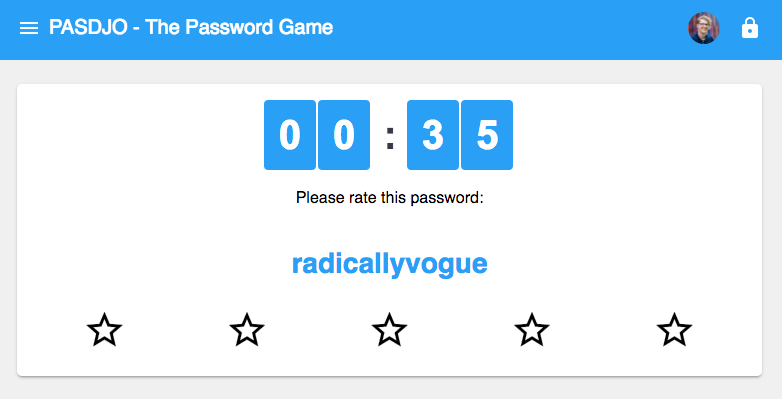
\includegraphics[width=0.75\textwidth]{pasdjo/radicallyvogue}
	\caption{\label{fig:pasdjo:radicallyvogue}}
\end{figure}

\subsection{Game Mechanics and Design Elements}
The game is relatively simple: Players judge how strong or weak a given password is. They receive points by accurately estimating the strength of a given password on a scale from 1 (weak) to 5 (strong). The game follows similar design strategies for the password topologies as the Ur \etal's online study, but passwords are either randomly taken from large dictionaries or generated on the fly. To induce intuitive estimations, a time-limit is enforced while a ``highscore'' acts as incentive to estimate as accurately as possible. To reach higher scores, one has to judge as many passwords as possible in 60 seconds. 

\subsubsection{Scoring and Metrics}
A crucial point of the game is how the passwords are rated objectively. Here, we rely on the zxcvbn library\footnote{\url{https://github.com/dropbox/zxcvbn}} (described in detail in Section \ref{sec:rw:pw_strength_metrics}) because it is highly reliable and straightforward to use on a web page. It also comes with a number of word lists that are helpful to implement different scenarios, respectively conditions. Beside the guess-number metric, zxcvbn also scores passwords on a scale from zero (weak) to four (strong). We translate this scale to one star (weak) to five stars (strong) in the game. 

For a correct estimation -- ``correct'' in the sense that zxcvbn comes to the same strength estimation -- a player is awarded 100 points. The difference between the user's rating and the zxcvbn score is  the \textbf{\textit{deviation}} ($D$). A player's rating can deviate by at most four stars, e.g. if they rate a five-star password with a score of one and vice versa. In that case, the player should not get any points, but in all other cases, the player is still awarded fewer points. For each integral deviation in either direction there is a penalty of 25 minus-points (maximum of 100 points, at most 4 errors, which leads to $100 / 4 = 25$). The points of the estimations are summed up and build the \textbf{\textit{achieved}} score ($A$). As an overall accuracy measure, at the end of the game we calculate the ratio of achieved and possible points and display it as percentage ($P$). 

The game thus implements the following scoring function, where $U$ is the user's estimation on a scale from 1 to 5, $Z$ is the zxcvbn score on the same scale, and $n$ is the number of passwords a user has rated within the time limit. 

\noindent The scoring function takes an array of user ratings and zxcvbn scores for $n$ passwords and returns a vector consisting of the achieved points $A$ and accuracy metric $P$.
\[
f([(U|Z)_1, ..., (U|Z)_n]) = (A|P)
\]

\noindent For each estimation the deviation from the zxcvbn score is calculated.
\[
D_k = U_k - Z_k\\
\]

\noindent The total achieved points are the sum of the achieved points per round. Each round takes the 25 point penalty into account. If $|D_k|=0$, the player gets the full 100 points per round.
\[
A = \sum_{k}^{n} 100 - (|D_k|*25) \\
\]
\noindent Finally, the accuracy is the fraction of achieved and possible points. 
\[
P = \frac{A}{n * 100}\\
\]

The score and accuracy are displayed to the users once the game is finished, see Figure \ref{fig:pasdjo:feedbackscreen}.

\begin{figure}
	\centering
	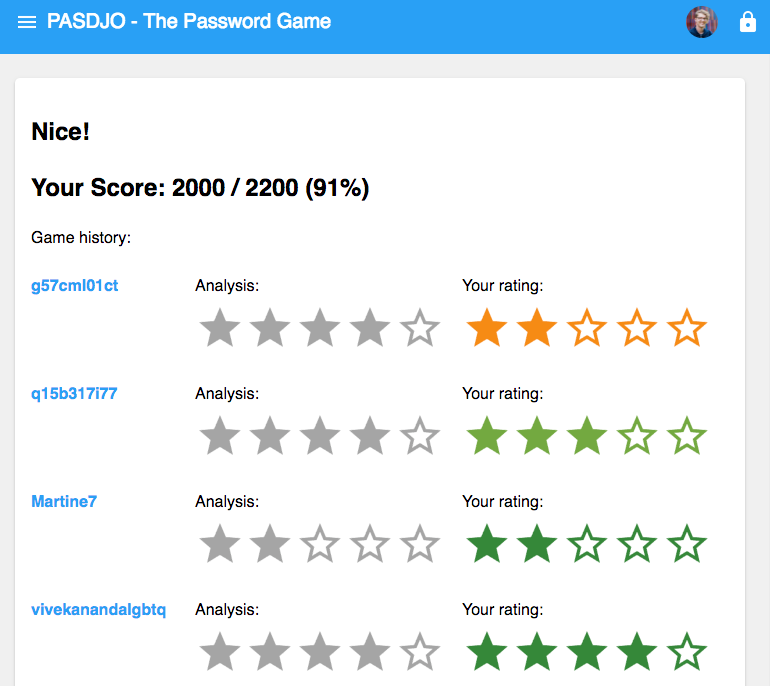
\includegraphics[width=0.75\textwidth]{pasdjo/feedbackscreen}
	\caption{\label{fig:pasdjo:feedbackscreen}}
\end{figure}

\subsubsection{Persuasive Design Elements}
discuss: 

low barrier to play the game: easy to understand, only takes one minute (persuasive weapon: commitment, small favors)
motivation: you might learn something or you can evaluate if your knowledge is correct (persuasive weapon: authority zxcvbn tells you what's correct) and discuss with other people. you can challenge your assumptions. 

we could also argue with Fogg Behavior model. 

%TODO Persuasive patterns (re Nicolas' comment at OzCHI)

\subsection{Password Generation and Study Conditions}
\makeatletter
PASDJO initially had four different password types that act as levels of the independent variable: Common passwords, mangled passwords, passphrases, and random passwords. During gameplay, the condition for the next password was selected at random. The following paragraphs depict the conditions in detail. 


\textbf{Common passwords: } We take the word lists that come with the zxcvbn library. One of these lists contains 47023 leaked passwords ordered by frequency, from which we randomly pick one for this condition. The data stems from breaches of user databases at RockYou, Yahoo and Xato \cite{Wheeler2016zxcvbn}. All passwords are lower-case and can be considered weak, because they are usually amongst the first attempts in a guessing attack \cite{Ur2015MeasuringRealWorldAccuracies} unless the adversary launches a targeted attack where personal information plays a more important role. Zxcvbn rates the top 1000 passwords with a score of 1 (e.g. ``12345'', ``password'', ``monkey''), and the remaining passwords are scored with two stars (e.g. ``iloveyou2'', ``skywalker'', ``apollo13''). It is worth noting that many of these passwords would not be accepted anymore by websites as common policies demand at least 8 characters (see Chapter \ref{chap:policies-reuse}), which RockYou and Xato did not enforce at the time. %TODO the last remark could go somewhere else. 


\textbf{Mangled passwords: } For the mangled password condition, we take the same list of the top 47023 passwords, but we algorithmically substitute certain characters. The substitutions look like ``leet''  / ``l33t'' speak, which is a typical way to try to increase password strength \cite{Das2014TangledWeb, Mazurek2013Measuring}. For instance, an ``a'' is replaced by an ``\@'', or an ``s'' is substituted with the dollar sign ``\$''. Also, random characters are transformed to uppercase. To allow recognizing the original word, we only mangle up to 30\% of the characters of the password. Since we only use substitutions that zxcvbn recognizes, mangled passwords mostly receive a score of two. However, in rare occasions, they occupy the full range, i.e., ``p@ssw0rd'' (1), ``b0n3he@d'' (2), ``fireFI9hter'' (3), ``123qaz456w\$x'' (4), ``123Q@z4s6w\$x'' (5). 


\textbf{Random passwords: } We implemented a simple string generation algorithm to create random passwords. They are lowercase alphanumeric passwords containing letters from the German alphabet, i.e. [a-z0-9äöü]. Zxcvbn consistently gives them a score of four, which makes them easy to rate. In a real-world attack they can only be brute-forced \cite{Florencio2014AdministratorsGuide, Wheeler2016zxcvbn}.


\textbf{Passphrases: } We combine two entries from the English Wikipedia index to create a passphrase (also shipped with zxcvbn). The words were required to be between 4 and 11 characters long. This restriction leads to a dictionary size of 27202 entries. Thus, there are $27202^2 \approx 10^9$ possible combinations, which is unpredictable enough to withstand online guessing attacks. This is reflected by the rather high scores: zxcvbn gives passphrases mostly a score of three or four, e.g. ``armedtamils'' (3), ``boostedeuros'' (4). If the words appear in other dictionaries, e.g. the ``TV subtitles'' word list, they are more likely to result in a score of three. However, for a user it is not straight-forward to tell whether a passphrase scores three or four points, which makes this condition harder to get right. 

\vspace*{2ex}
For the remainder of the chapter we refer to these four condition as ``Common'', ``Mangled'', ``Random'', and ``Passphrase''.


\subsection{Benefits and Shortcomings of the Game-based Approach}
Since the game was deployed publicly, the method can be denoted as an unsupervised in-the-wild study. This approach has certain benefits and shortcomings as discussed in the following. 

\subsubsection{Benefits}
\textbf{Easy collection of multiple data points per user} The game can be played over and over. A survey could also be taken multiple times, but most of the time this is not desirable. If the study is done via MTurk this would mean that people would be paid each time which drives costs.

\vspace*{1ex}
\noindent\textbf{Possibility to provide feedback} After the game, the players can review their ratings and find out how they performed. In a study, implementing such a feedback loop is much more complicated and often impossible with current survey tools. Hence, a debriefing step is required, but it's difficult to tailor it to the individual participant.

\vspace*{1ex}
\noindent\textbf{Randomization and password space} Ur \etal's study was designed well in that it tested a wide range of password characteristics and there were multiple options per condition. However, the options were predefined by the researchers and limited in that sense. In our case, we can pick passwords from much larger word-lists at random and use algorithms to randomly adjust certain characteristics. This allows for higher internal validity of the data collection.

\vspace*{1ex}
\noindent\textbf{Intrinsic Motivation} The game is 

\subsubsection{Drawbacks}

Lack of demographics

playing on multiple devices is hard to trace

disclaimers are somewhat hidden as a trade off of lowering the barrier to play the game

\subsection{Implementation}
polymer firebase webpage PWA 
UX considerations: load quickly, run offline and large data transfer (mobile first paradigm), disclaimers
\section{Log Analysis}

\subsection{Sample}

December 2016 until March 2017
two important events: Open Lab Day of our research group and student orientation day at LMU central
Thus, it is likely that most players were students or in academia. 

What data did we throw out and why? how much of the dataset is that?

\subsection{Results}

%TODO consider running another test a year afterwards.


\section{Discussion}

\subsection{Strength Perception vs. Selection}
- perception and estimation of password strength appear to be easy for the players of our games even if they might not have a background in cyber security. 
- you rarely see passwords of other people, only when they share it with you. In many cases passwords that are shared with you are typically not the strongest passwords \cite{Haque2014Hierarchy,  Shay2010EncounteringPasswordRequirements, Singh2007PasswordSharing, Violettas2014PasswordsAvoidGreece, Weirich2001PrettyGoodPersuasion, ZhangKennedy2016RevisitingPasswordRules} 

\section{Limitations}
\begin{itemize}
	\item were already addressed in new versions of the game. 
	\item used as an activity at Google	
\end{itemize}


\section{Summary}
\begin{itemize}
	\item users performed better than anticipated
	\item misconceptions mainly involve passphrases and mangled passwords
	\item the game was updated after the first results were in and is still deployed. Google even uses it internally. 
	\item the source code is available on GitHub.
\end{itemize}

\section{Improvements in Revisions}
see slides from talk
updated scoring
more evenly distributed scores and conditions
updated passphrase generation algorithm (not just two words, but randomly 2 or 3, random punctuation)
leaderboard (game design element)

\subsection{Future Work}
Better onboarding
Challenges
Player Profiles 
adding the game to password management software

 %published
%%!TEX root = ../../diss.tex

\chapter[Field Study: Authentication Time]{Field Study: Authentication Time}\label{sec:auth_time}

\section{Background and Context}
\section{Results}
\subsubsection{TODO}
 \section{Password Habits}
A lot of Herley and Florencios work focused on quantifying the ``password problem'' as an everyday task (@REF SEC RW). However, the studies were conducted almost a decade ago. @TODO elaborate on argument: More internet services, rejection of SSO etc.

We have therefore reason to believe that the amount of accounts has increased compared to the 2000s. As such, we hypothesized that users face a higher number of authentication tasks, in particular with passwords on the web, each day. 


\section{Password Managers}

\subsection{Criticsm}
\begin{itemize}
\item[Leakage] LastPass breach in 2015 \footnote{https://blog.lastpass.com/2015/06/lastpass-security-notice.html/, last access March 30 2016}
\end{itemize}
 % can go 
\chapter[Mental Models of Password Managers]{Mental Models of Password Managers}\label{chap:mental_models_pwm}
%lingo: prospective users.
An important spillover of our previous exploration is that password managers are more likely adopted the longer people had struggled with juggling passwords: Older participants in the third personality study were more likely to use a \gls{PWM}. We have already corroborated market surveys that indicate a generally low adoption rate of password management software. As discussed in Sections \ref{sec:rw:user-behavior} and \ref{sec:rw:pwm_generators}, it has been hypothesized that users do not fully trust third parties with their credentials, so there seems to be an urge to stay in charge. Consequently, most users still try to memorize their passwords. On the other hand, password managers do provide many usability and security benefits, but why do users fail to see them? To this end, we see a lack of understanding about how users make sense of password managers. Our goal was to understand users' mental models of password managers first and then identify opportunities to improve them, which could increase adoption rates. 
%RQs
We thus aimed to answer the following research questions: 
\textbf{(1)} How do users think a password manager works? 
\textbf{(2)} How does adopting a password manager change user attitudes and behaviors?


To answer these questions, Martin Prinz and I explored attitudes and understandings in semi-structured qualitative user interviews. To get a more complete picture, we interviewed both people who already use a \gls{PWM} and also people who prefer other coping strategies. Parts of the outcome of this investigation have been published as an extended abstract at SOUPS 2017 \cite{Prinz2017MentalModel}.

\section{Background and Context}
%%%
% technical side
%%%

% PWM have existed since xyz. -- not possible to point a specific origin. 
Password managers can be either built into web browsers or act as a standalone solution that is independent of the password's purpose. Dedicated password managers have existed since the mid to late 1990s. Web Confidential\footurl{http://www.web-confidential.com/}{16.02.2018} was probably one of the first programs to facilitate password management, when it first surfaced in 1998. However, which of the browsers was first to add password storage capabilities cannot be easily traced back, but all major browsers added this feature in the early 2000s. Given the long history of supporting authentication with software tools, adoption of password managers is still at only 12\% \cite{Olmstead2017AmerciansCybersecurity}. Even security experts disagree on the specific security benefits of different implementations\footurl{https://www.wired.com/2015/07/websites-please-stop-blocking-password-managers-2015/}{16.02.2018}. If the auto-fill feature is enabled, this can be used to create digital footprints for individuals\footurl{https://freedom-to-tinker.com/2017/12/27/no-boundaries-for-user-identities-web-trackers-exploit-browser-login-managers/}{16.02.2018}. Nevertheless, similar attack vectors could easily target regular password entry, and are not limited to auto-fill. 

% different system architectures: built into browser, local software (dedicated programm and/or browser extension), distributed storage.
There are different service architectures for handling passwords: \textit{offline} password managers keep a database of encrypted passwords locally on the user's machine, while \textit{online} managers provide more mobility because passwords are held on a server or a distributed storage solution \cite{McCarney2012Tapas}. \textit{KeePass} and \textit{Password Safe} are notable representatives for the offline storage paradigm, while the cloud-based approach is dominated by third-party solutions like \textit{LastPass}, \textit{1Password}, and \textit{Dashlane}. Browser vendors have also transitioned to store passwords in the cloud, e.g. Apple Keychain for Safari, or Google Smartlock for Chrome. On the one hand, this provides consistent user experiences across multiple devices. On the other hand, such architectures create lock-in effects and dependencies. Thus, online password managers typically provide browser-extensions to automatically fill username and password fields. This way, similar experiences are achievable by third party tools. 

% pwms are not universally accepted as the best solution.
% some websites block password managers (by disabling the ``paste'' event on their login form), because under some circumstances password managers can be used to track users. 

%%%
% user side:
%%%
% academic

% briefly summarize experiments focused around mental models of password managers
\paragraph{Mental Models} 
%motivation
Norman suggests that exploring mental models provides predictive and explanatory power for understanding an interaction \cite{Norman1982ObservationsMentalModels}. Volkamer and Renaud meticulously described different aspects and definitions of mental models, which are too elaborate to discuss in this work \cite{Volkamer2013MentalModels}. As a takeaway, a mental model describes a user's sense-making of any system they interact with. Volkamer and Renaud highlight that mental models are not necessarily static, but can be shaped with different cues to internal feedback loops (see Figure \ref{fig:mm_pwm:mental-model-volkamer}). For our purposes, we use a simpler definition provided by Young: Mental models are ``collections of the root reasons why a person is doing something'' and ``represent what a person is trying to accomplish in larger context, no matter which tools are used''  \cite[p.11]{Young2008}. In our case, they describe the reasons for (not) using a password manager, as explained by current actions to cope with authentication tasks. 

\begin{figure}
	\centering
	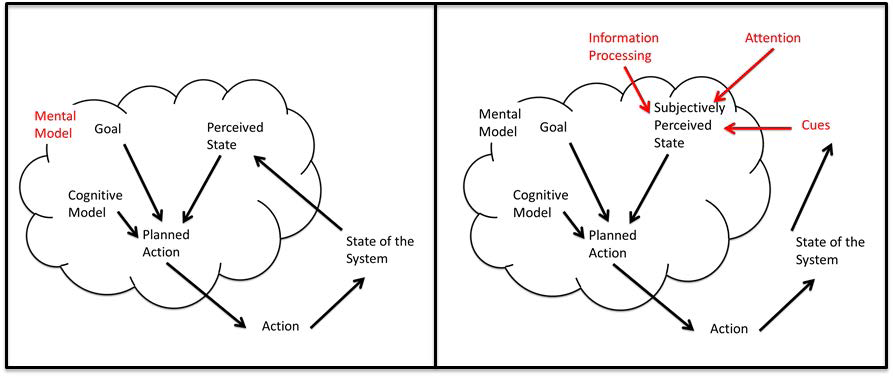
\includegraphics[width=\linewidth]{mm_pwm/MentalModels-volkamer}
	\caption{\label{fig:mm_pwm:mental-model-volkamer} Volkamer and Renaud see the formation of mental models as loop involving different plans, perceptions, system structures, and actions. Image from \cite{Volkamer2013MentalModels}}
\end{figure}
% what is different now? quant --> qual
In chapter \ref{chap:pasdjo}, we took a quantitative approach to elicit data on the mental models. This was useful because we tried to understand \textit{what} contributed to password strength perceptions and by \textit{how much}. For password managers, related work on usage motivation is scarce, thus we strove to answer \textit{why} users perform certain actions and \textit{how} these could be supported by a password manager. Therefore, qualitative methods were more useful. 
% how is this qual data elicited?
Eliciting such data to understand mental models, Bravo-Lillo \etal relied on open-ended one-on-one interviews both with advanced and novice user groups \cite{BravoLillo2011WarningsMentalModel}. They highlight the usefulness of this approach to understand thought processes. Kang \etal relied on \textit{drawing tasks} to elicit additional data \cite{Kang2015MentalModelsDrawing}. Participants were asked to sketch what they thought happens to their personal data when they interact with different online services. During sketching, a \textit{concurrent think-aloud protocol} was used to avoid misunderstandings. Once the data has been collected, Young suggests the \textit{affinity diagramming} method to derive themes and identify opportunities for supporting tasks \cite{Young2008}. In this research project, we combined interviewing, drawing tasks, and affinity diagramming. 

\section{User Interviews}
Our main objective was to understand how users make sense of password support tools, in particular password managers. This would allow us to explore solutions that fit user expectations better.  

\subsection{Method and Protocol}
Focusing on attitudes and mental models requires a qualitative study method. We chose to conduct semi-structured, open-ended interviews. The sessions started with a thorough briefing about the study purpose and asking for permission to audio-record the conversation. The main questions were \textbf{(1)} \textit{Why do you need passwords?} and \textbf{(2)} \textit{What is your strategy to manage multiple accounts?}. From there, the study followed a more fine-grained follow-up questions to investigate the specifics of these two aspects. Moreover, Bravo-Lillo \etal showed the benefits of drawing tasks to find structural patterns in beliefs \cite{BravoLillo2011WarningsMentalModel}, so we also asked participants to \textbf{(3)} \textit{sketch how a password manager works}. This required that participants were aware of \glspl{PWM}. If they were not, they were told that it is a ``piece of software that stores a user's password'', which was expected to be vague enough to explore participants' expectations of this kind of software. The interviews took between five and 16 minutes. 

\subsubsection{Recruitment and Sample}
We first approached random passers-by on a popular street in Munich to obtain a diverse sample of participants. Six interviewees were recruited this way. However, these first six interviews showed that participants were unable to provide sufficient detail in answers to allow thorough analysis. Thus, we changed the recruiting method and approached employees of a design agency with which we had collaborated in the past. We also knew that the agency's policy required employees to utilize password managers. Moreover, the user group was more likely capable of visually expressing mental constructs, allowing for the envisioned analyses. Eight additional participants were interviewed in this sample, giving a total of N=14. They worked as experience designers and concept developers, and did not have formal training in computer science or engineering. The age of all interviewees ranged from 20 to 41. \todo{listen to recordings and determine gender distribution (CD in Munich)}. 

None of the interviewees in the first group had used a password manager before, so we call this participant group the \textit{novices}. Since the \gls{PWM} was part of the company policy, all interviewees in the second group had used one before, so we call them the \textit{actives}. The separation allowed us to detect a shift of expectations before and after adopting a password manager. 

\subsubsection{Method Limitations}
The recruiting and sampling methods are inherently limited. The novice user group was asked at a public spot, so it was difficult to provide enough context information and minimize distraction. On the plus side, we achieved diversity and the face-to-face set-up reassures trust, because it was clear that none of the information they gave us was going to be used to access their online accounts. 5 of 6 \textit{novices} were unable to describe what a password manager was, before we gave them the above definition. Thus, their decision to refrain from using a \gls{PWM} was not made actively, but rather results from the lack of awareness. This limits the analysis of attitudes and self-reported behavior. Finally, the second user group has a homogeneous background: design and communication. All these limitations demand that the results not be generalized to a larger population. Instead, they should be seen as rough trends that help understand a first set of underlying mental models, rather than the entire spectrum thereof.

\subsection{Data Analysis and Results}
% analysis approach
Young proposed a design strategy to translate qualitative data into mental models \cite{Young2008}. The method is based on \textit{affinity diagramming}. The resulting clusters and themes from the diagram are then mapped to a hierarchical structure that consists of Mental Spaces, Task Towers, Tasks, and Particular Tasks. Here, we focused on those Mental Spaces and Task Towers that involve password managers. Table \ref{tab:mm_pwm:mental-model-table} shows the resulting model in this format. In the following, we report the results that notably contributed to the formation of the model, which is described in Section \ref{ref:mm_pwm:mm-description}.

\begin{table}[htpb]
\def\arraystretch{1.05}% 
\begin{threeparttable}
\begin{tabular} {l|l|l}
\textbf{Mental Space} & \textbf{Task Tower} & \textbf{Tasks} \\ \hline\hline
Creation \& Selection
& Influential Factors & Personal \& Historical \\ 
& & Policies \& Rules \\
& & Algorithmic Strategies \\
& & Account Context \\
& & Memorization \\ \cline{2-3}
& Support Tools & Generate \& Memorize \\
& & Use given Password \\
& & Generate \& Digitally Store \\ \cline{2-3}
& Personal Algorithms & Passphrases \\
& & Reuse Word Blocks \\
& & Base-Password with Modifications \\
& & Website Influence \\
& & Use Reduced Alphabet \\\cline{2-3}
& Handle Failures & Trial and Error \\ 
& & Lookup Password \\
& & Show Entered Password in Plain Text\\
& & Reset Password \\ \hline 
Log-In 	& Manual Tasks 	& Copy \& Paste password \\
	 	& 		 	& Lookup hints and cues \\ 
	 	& 		 	& Recall from memory \\ 
\cline{2-3}
		& Simplify 	& Stay logged-in \\ 
		& 			& Cross-device support \\ 
		& 			& Autofill forms \\ 
		& 			& Rely on manager \\ \hline
Organize and Commit & Share Passwords & Secure sharing with colleagues or friends \\
		&			& Write down password \\
		&			& Reset after sharing\\ \cline{2-3}
		& Use Aid & Password Manager \\
		& 		 	& Word/Digital Document \\ 
		& 		 	& Handwritten Notes \\  \cline{2-3}
		& Memorize Passwords & Algorithmic \\ 
		&			& Website Cues \\
		& & Mental Drawer \\
		& & Base Password and Modifications \\ \cline{2-3}
		& Protect Passwords & Modify Passwords \\
		& 			& Unlock access with Master Password\\
		&			& Hide or Encrypt File/Notes \\ \cline{2-3}
		& Automation & Reset Multiple Passwords\\
		&  			& Autosave Credentials \\ 
		&			& Autofill Username and Password \\
		&			& Warnings when websites are compromised \\\cline{2-3}
		& Build Password Categories & Security \\ 
		&			& Importance \\
		&			& Frequency \\
		&			& Policies \& Rules \\
		&			& Mental Drawer \\ \hline

\end{tabular}
\end{threeparttable}
\caption{\label{tab:mm_pwm:mental-model-table}
	Mental Model of Authentication and Password Management, adapted from Martin Prinz \cite{Prinz2017Thesis}}
\end{table}% \ref{tab:mm_pwm:mental-model-table} %
%\begin{figure}
%	\centering
%	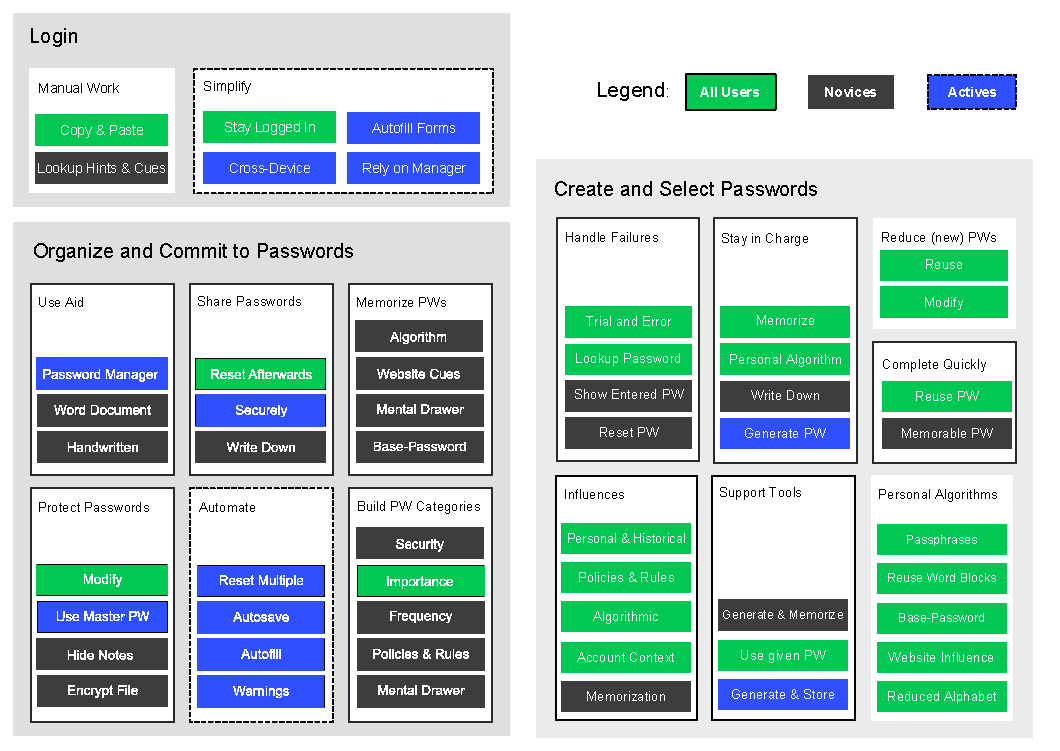
\includegraphics[width=\linewidth]{mm_pwm/mental-model-diagram}
%	\caption{\label{fig:mm_pwm:mental-model-diagram} Mental model diagram}
%\end{figure}


\subsubsection{Selection and Coping Strategies}
All interviewees reuse passwords to cope with the multitude of accounts. Participants often developed coping strategies without deliberation: they were unaware of how they cope with passwords until we specifically requested more details. Only then did they reflect and realize how they behave. One such revelation was that they categorize passwords in different ways. For instance, the context in which they created an account, e.g. the URL or policy of the corresponding website, was factored into passwords and facilitated the decision-making process which password to choose from their portfolio (see Figure \ref{fig:mm_pwm:creation-strategies} A). Similarly, the perceived importance led to distinct categories, although the interviewees had not realized this. Furthermore, we also heard an interesting, deliberate strategy that seldom appears in the literature: two participants mentioned memorizing a list, or a list of letters that are then transformed into a new, quasi-unique password. This method is comparable to the Diceware technique (see \ref{sec:rw:passphrases}), but instead of rolling a dice, these participants algorithmically select the order of words/letters based on contextual cues (see Figure \ref{fig:mm_pwm:creation-strategies} B and C). Another participant said to have memorized a randomly generated password and reusing it many times. Finally, participants generally tried to justify their ``insecure'' behavior. Beside memory burden of new secrets, time pressure was mentioned as reason for password reuse. 

We also inquired situations when their strategies failed. The primary problem of having a multitude of accounts was the correct \textit{combination} of user-name and password, which is a common pitfall of knowledge-based authentication \cite{Stobert2014PasswordLifeCycle}. Not only did they forget passwords, but also user names, which is just as severe because web sites generally do not inform users which was the error source to thwart attacks. Participants reportedly use a trial-and-error to go through their portfolio and ultimately use self-serviced password resets as a convenient solution. Interviewees expected that websites offer this kind of fallback scheme, because two of them do this on a regular basis. 

\subsubsection{Password Manager Impact}
Overall, the \textit{novices} and \textit{actives} did not behave differently in their selection and coping strategies at first sight. However, we found that \textit{actives} did in fact change some habits when they had started using a password manager. First, although they were initially exposed to \glspl{PWM} at work, \textit{actives} started using them in private shortly afterwards. This interaction and experience with the tool led to their migrating passwords into the manager step by step. One participant mentioned that it helps him stay organized where there was ``chaos'' before (see Figure \ref{fig:mm_pwm:creation-strategies} C). Others were somewhat ashamed of their weak practices before using this kind of software. 
Password sharing with other users was the central advantage for four interviewees, especially at work. It facilitates secure collaboration with colleagues and clients. Participants do not memorize these passwords, because they often use built-in password generators. They realized that shared passwords are short-lived because colleagues leave or contracts with clients end, upon which passwords are invalidated. One interviewee fully embraced generated passwords even for private purposes and only memorizes his master password. Interestingly, however, for their most important accounts, most \textit{actives} kept on manually crafting passwords and refrained from putting them into the \gls{PWM}. Having used the tool and become aware of their own weak behavior in the past, they had gained confidence in selecting stronger passwords. This gain of mastery left them with a positive experience of password managers. As a contrast, \textit{novices} were all comfortable with how they managed their passwords and did not show that sense of insecurity.

\begin{figure}
\centering
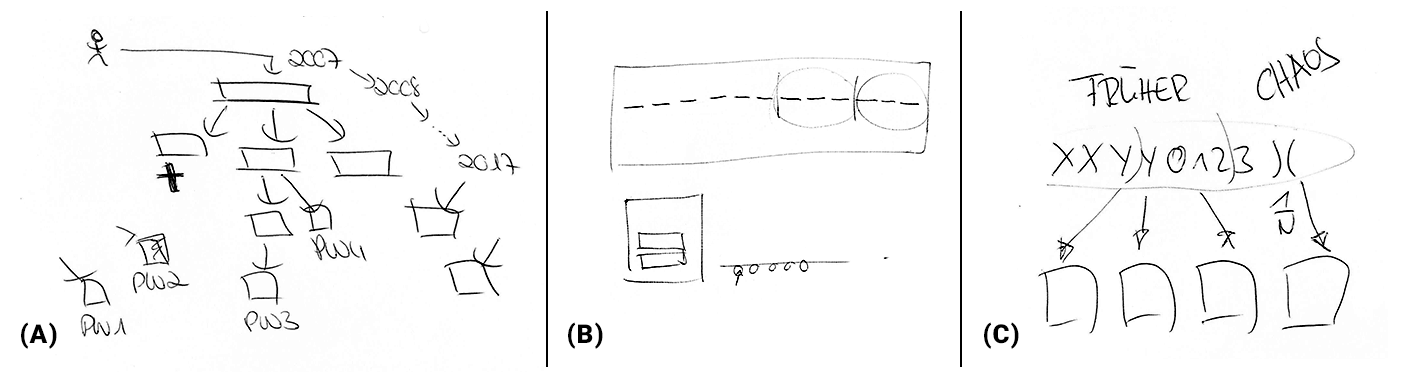
\includegraphics[width=0.9\linewidth]{mm_pwm/f_creation_sketch}
\caption{\label{fig:mm_pwm:creation-strategies}	Participants were asked to visualize their methods to create passwords, if they had a specific strategy. (A) participant who categorizes and remembers passwords by the time they were created (context factors). (B) participant uses words and cued positions to recall the constellation. (C) participant who uses a fixed set of characters and algorithm to ``calculate'' the correct constellation.}
\end{figure}

\subsubsection{Drawing Tasks}
Participants were asked to sketch their thoughts whenever this was appropriate. We encouraged them to sketch as much as possible. All participants mentioned that it was challenging to communicate their understanding this way. Already for basic functionality and purpose of passwords, we asked to create sketches. This task was still relatively easy for all interviewees. Padlocks and keys were two of the most commonly drawn elements. It also helped to communicate individual elaborate selection strategies (see Figure \ref{fig:mm_pwm:creation-strategies}). However, the difficulty rapidly changed for the workings of a password manager.
Here, especially \textit{novices} struggled with the task and could not proceed without further explanation, and their drawings were more vague than those of \textit{actives}. However, the latter is probably due to the different professional background and expertise in creating concepts. The drawn elements and metaphors differed among the two groups: 
\paragraph{Novices} had a vague model of how such a password manager might work and found it especially difficult to sketch this. The benefits and system architecture of the software were unclear to them. One interesting drawing depicted a password manager as a virtual ``brain'' that acts as a central hub to make the user's life easier (Figure \ref{fig:mm_pwm:f_novice_sketch} B). Another participant, who reportedly used a Word document to keep track of his accounts, imagined a password manager to behave the same way (Figure \ref{fig:mm_pwm:f_novice_sketch} C). The only expected difference would be that accessing the list of passwords would be protected by a password, which is indicated by the keyhole and an arrow that points to it. This represents \textit{novices'} understanding on a more general level, as they explained a password manager as a special way to manage a \textit{secure list of passwords} that helps find the right ones. Five said that it facilitates logins by allowing them to \textbf{copy-and-paste} passwords from the manager into the webpage. 
\begin{figure}
	\centering
	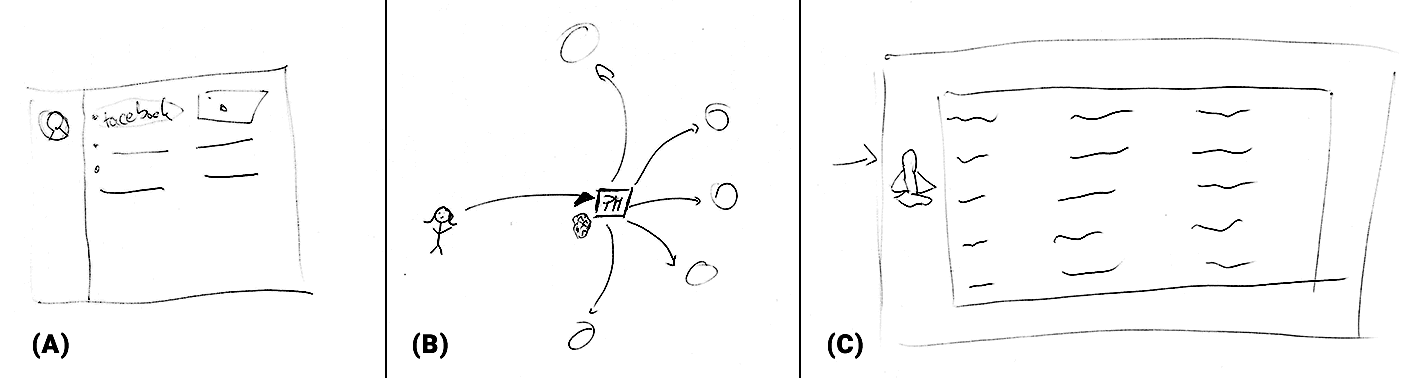
\includegraphics[width=0.9\linewidth]{mm_pwm/f_novice_sketch}
	\caption{\label{fig:mm_pwm:f_novice_sketch}	Drawings to the question ``What does a password manager do, and how?'' from three \textit{novice} users. (A) only shows a profile on facebook. (B) emphasizes that the PWM is a central hub and acts as the user's ``brain'' for different entities. (C) shows a table-like structure that holds all username-password tuples.}
\end{figure}

\paragraph{Actives} Since all active users were also visual communicators, it was somewhat easier for them to sketch the workings of a password manager. They clearly focused on the interaction between users and the system and highlighted the benefits in their drawings. Having experienced the advantages, they strove to convey these visually and came up with more details (cf. Figure \ref{fig:mm_pwm:f_actives_sketch1}). Instead of a password-table, we can see workflows that show the interplay between user, database and website. Common components are UI elements like input fields
or buttons that link to other screens or entities. Only one interviewee from the \textit{active} group refrained from UI elements and instead sketched a flow-chart. 
\begin{figure}
	\centering
	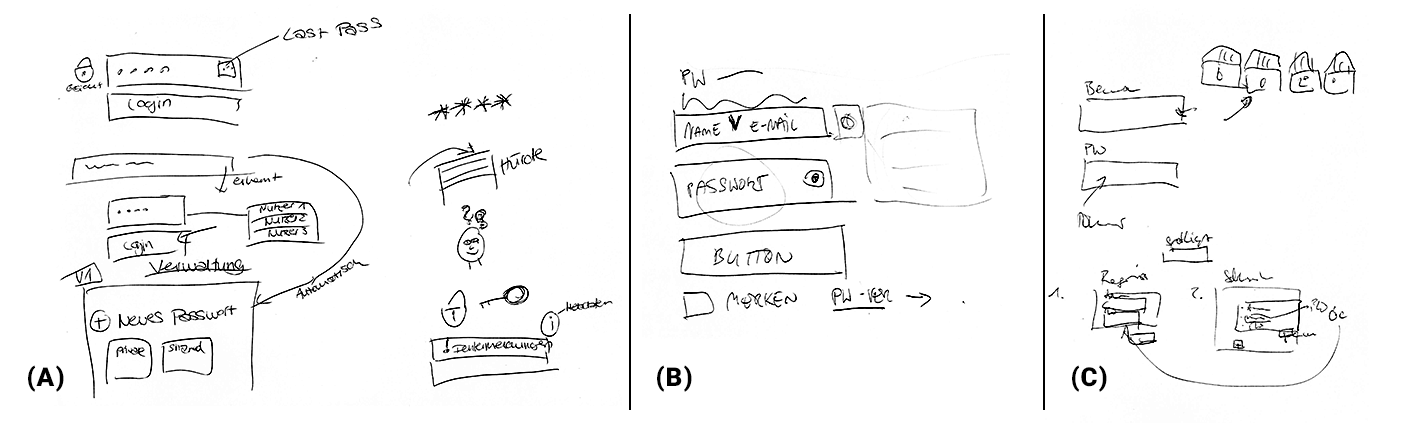
\includegraphics[width=0.9\linewidth]{mm_pwm/f_users_sketch1}
	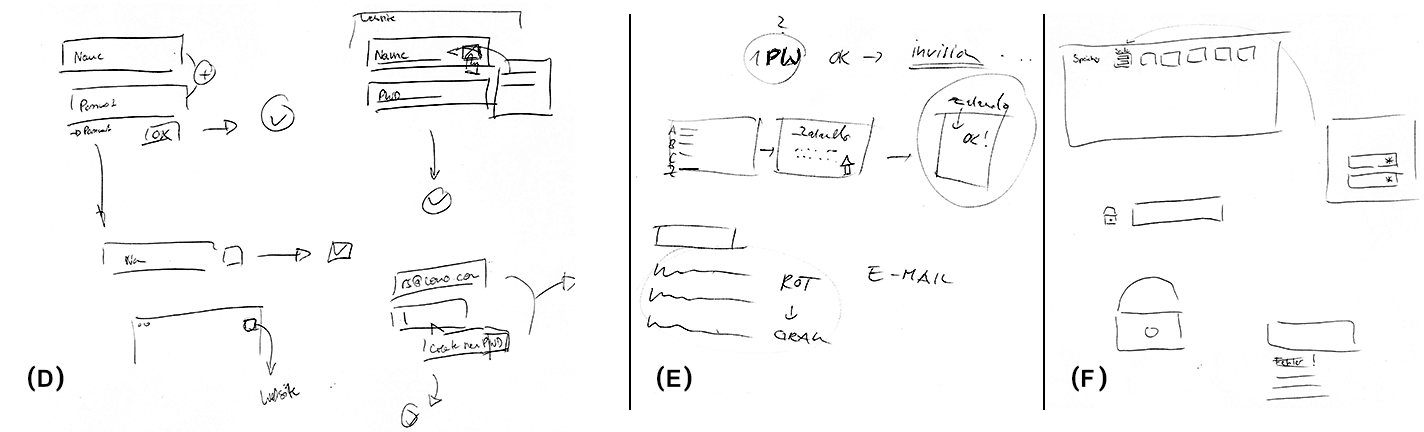
\includegraphics[width=0.9\linewidth]{mm_pwm/f_users_sketch4}
	\caption{\label{fig:mm_pwm:f_actives_sketch1} Drawings to the question ``What does a password manager do, and how?'' from six \textit{active} users. Common components are UI elements that link to other entities, therefore the interplay between user, PWM and website is clearer.}
\end{figure}

\section{Mental Model}\label{ref:mm_pwm:mm-description}
From the behavioral, attitudinal, and experiential data, we created a mental model schema in the style of Young \cite{Young2008}. We tried to stay close to the data as possible, but a few points are enhanced by knowledge from related work. We briefly elaborate on the mental spaces to allow the reader to delve into task-towers and tasks. 

\paragraph{Password Creation and Selection}
First, users have a variety of particular needs when they are challenged to create a password. This task tower describes both the constraints, prior experiences and strategies to accomplish the task. Our participants often mentioned highly individual selection strategies that allow for both secure and memorable secrets. From a support tool, they expected guidance and feedback. Password generators that simplify this task can aid here. 

\paragraph{Log In}
Most prominently, authentication still involves \textit{both} manual and automatic tasks. Interviewees expected to copy and paste passwords from the manager to their browser, or at least provide a way to retrieve password hints.  On the other hand, participants expected that support tools are deeply integrated into the browser by automatically filling password fields in a highly reliable manner. If possible, the solution should work across multiple devices. 

\paragraph{Organize and Commit}
The third mental space resembles the ``Commit to password'' and ``Live with password'' stages of the Password Life Cycle \cite{Stobert2014PasswordLifeCycle}. Each participant mentioned some way of organization strategy that allowed them to live without password managers to some degree. However, these were not always deliberate choices, but rather have formed over the years. Especially \textit{novice} users made sense of password managers by their capability of protecting passwords, i.e. encrypting a list of passwords rather than just storing them in a Word document. \textit{Active} users were already aware of the sharing capabilities and appreciate a simple process to reset passwords when they need to be invalidated for security reasons.

\section{Opportunities and Challenges}
Having fine-grained insights into the mental models of password authentication sub-tasks lets us explore novel ways to support users in many challenges. In the following, we highlight key opportunities for future work on password managers and password support in general. 

\subsection{Leveraging and improving novices' mental models}
There were two important preconceptions about password mangers on the \textit{novices} side: simple password lists and copy-paste interactions. Future password managers can leverage these models to persuasively communicate functionality. The value proposition should thus ensure that potential users understand that PWMs are \textit{not only} a secure list of user-names and passwords, but also help them \textit{select} passwords -- a benefit that \textit{actives} had realized in retrospect. The \textit{password list} metaphor is also useful to communicate automation features: explicitly showing new users that they do not have to search through the list, nor copy and paste passwords from the list to the website might help them understand the simplicity of the interaction paradigm. This can happen during an onboarding user journey, e.g. with an image showing the steps saved by the PWM (cf. Figure \ref{fig:mm_pwm:pwm-goms-comparison}).

\begin{figure}%TODO could make this a little bit nicer. 
	\centering
	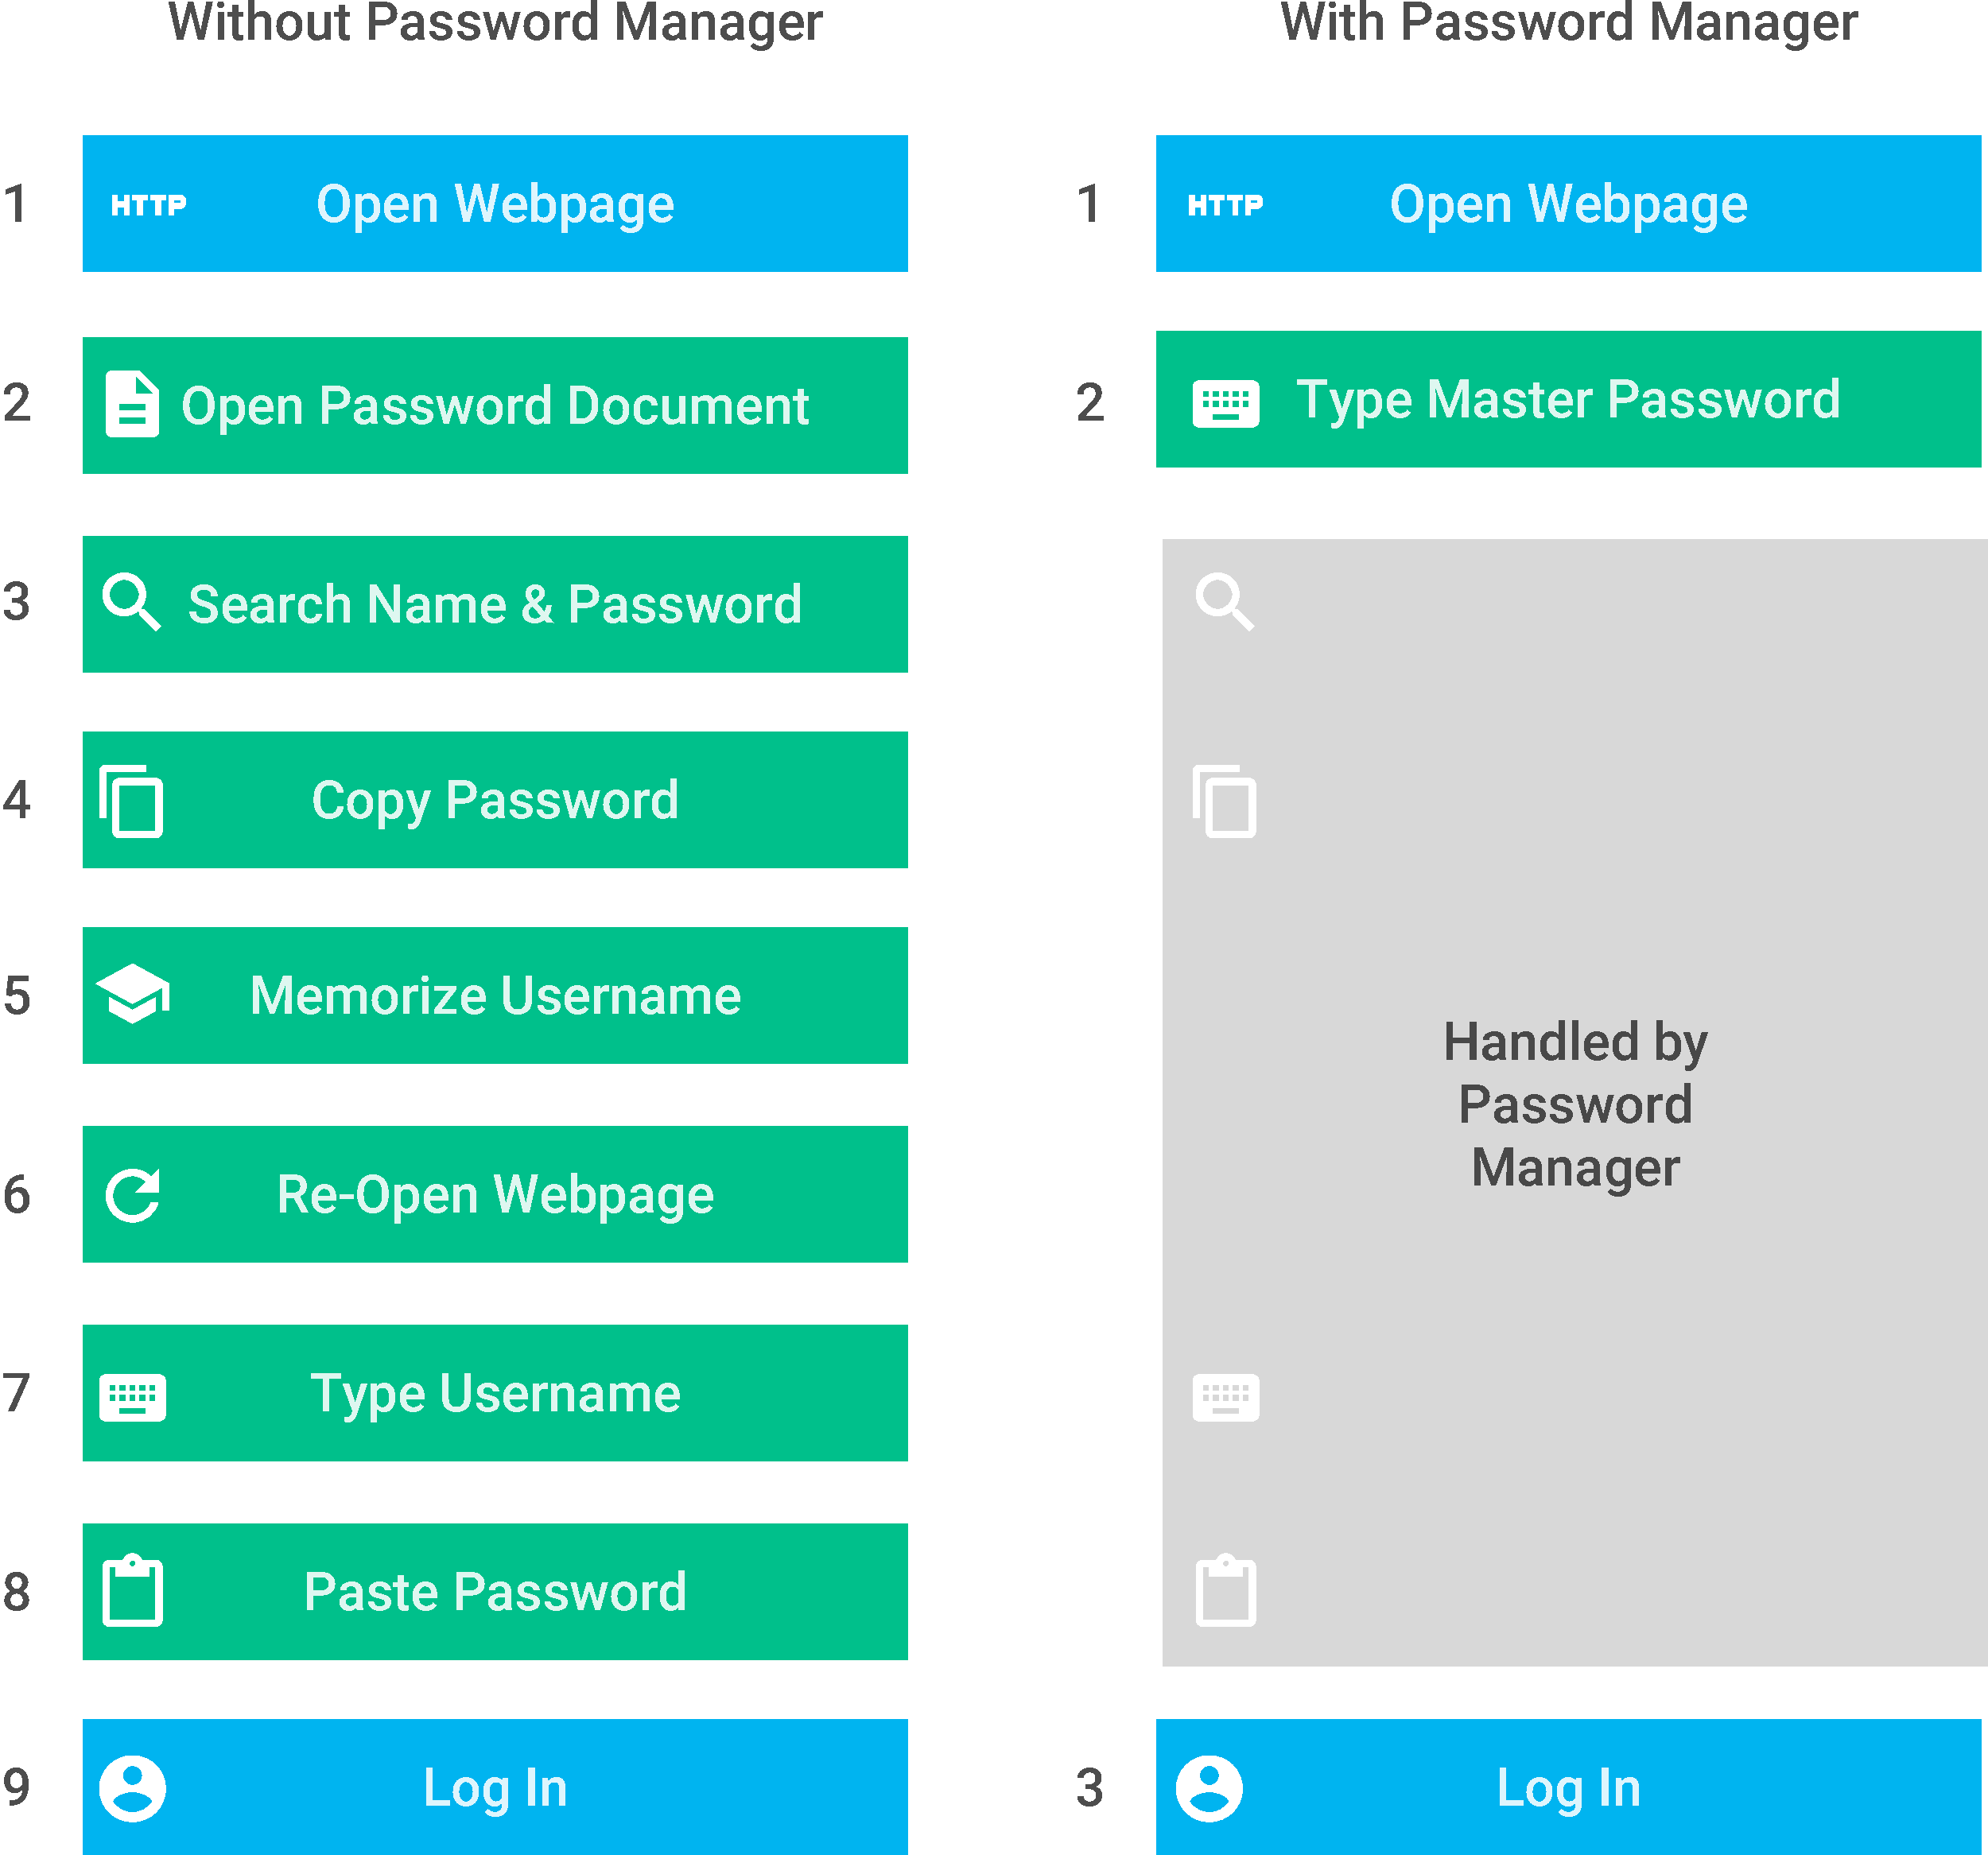
\includegraphics[width=0.6\linewidth]{mm_pwm/pwm-goms-comparison}
	\caption{\label{fig:mm_pwm:pwm-goms-comparison} Visualizing users' previous behavior might help communicate how the password manager can simplify authentication tasks. This can create a better mental model of their workings.}
\end{figure}

%- trust was not an issue because they were generally unaware of the existence of PWM.

\subsection{Increasing Sense of Agency}
While automation simplifies processes and thus improves usability, staying in control of security-related interactions is important to users. \textit{Novices} were confident in their current behavior. \textit{Actives} had realized that their past behavior was sub-optimal, but they had gained confidence to create passwords and handle authentication for their most important accounts on their own. As a consequence, a password manager needs to stay flexible enough to respect user preferences for different account \textit{categories}, e.g. unimportant vs. important accounts. At the same time, reassuring users that their decision to handle such situations on their own is reasonable and can inspire trust in the system. A PWM could automatically detect when it is appropriate to offer help. Current managers only provide the opportunity to decide whether the password should be saved, maybe saved later, or never be saved for a particular site. Such decisions can be automated once enough training data has been provided by the user.

\subsection{Leveraging Context}
Context factors can be leveraged by PWMs to adapt to different situations. For example, usage-context informs future interactions. If the user sets up the system at work, this is an indicator about how passwords are going to be categorized, how often they will be reset, and how likely they are going to be shared with others. Adapting the interface to such scenarios can simplify interactions and forming mental models of the benefits. Moreover, automated generation of passwords is also context-dependent. As we have shown in chapter \ref{chap:policies_reuse}, password policies in the wild impose varying restrictions on the use of characters. To avoid user frustration arising from rejected passwords, e.g. because they contain forbidden characters, the generator can ensure the random password meets the website's composition policy. 

%- onboarding process: usage at home or at work / customized/adaptive onboarding
%- better embedding in sign-up forms 
%- automatic password generation should consider password policy. --> see chapter \ref{chap:policies_reuse}

\subsection{Customization and Personalization}
It is evident that current third-party and browser-built-in password managers form a standalone mechanism that works differently compared to how users normally cope with passwords. Our participants reused passwords with different strategies and relied on digital documents, paper notes, and highly individual password creation or memorization techniques. Beside the document-metaphor discussed above, the other strategies are not reproduced by password managers. However, a general philosophy in user-centered design is the aim to ``fix the system'' rather than to ``fix the user''. Therefore, the system should provide ways to support current strategies. For instance, it could help the user specify their creation technique: they might use a base-password that is modified depending on the context, the PWM could offer to generate passwords like this in future scenarios. While this approach would not necessarily improve security, it could save the user time and make authentication more usable. Besides, the user stays independent of the tool, because they can reproduce their system and log in on other devices even without the support. 

%- current pwms do not support many behaviors that users still do: reuse, word documents, paper notes, individual creation and memorization techniques, reuse strategies. 
% - maybe target persona elliot elis

%\subsection{Limitations}

\section{Conclusion}
We explored the mental models of authentication tasks and password managers with a qualitative approach. Both participants experienced with password managers and inexperienced novices shared their insights, attitudes and behaviors during short interviews. Fourteen interviewees provided us detailed descriptions of their password selection and coping strategies, and how they make sense of supporting tools. 
% how does this change the world?
We contribute evidence that (a) individual coping strategies persist even after adopting a password manager for important accounts, (b) work environments serve as onboarding triggers even for private use, and (c) novices were mostly unaware of the functionality and benefits of password managers. 
% larger vision.
These findings show that the value proposition should be communicated concisely and compare the benefits against inefficient password practices. At the same time, new solutions should respect highly individual coping strategies to better match user behavior. Ultimately, this could increase adoption, and more importantly, retention rates. 


\noindent
\fbox{
	\hspace{1cm}
	\parbox[c][12cm]{0.7\linewidth}{
		\section*{Take Aways}
		\begin{itemize}[leftmargin=*]
%			\item The system architecture of a password manager is difficult to frame visually both for people who have never used one, and also for users. Active users created more visually rich sketches, but this was likely due to their professional background. 
			\item Password managers appear to be a ``black box'' for people who have never used one. They suspect that such tools are a slightly more secure version of text files to write down lists of username-password-combinations.
			\item The mental model of password authentication and managers is mostly divided into the mental spaces ``Select password'', ``Log in'', and ``Organize''. There seem to be discrepancies between current user behavior and current password managers. 
			\item Making password managers adapt to context and individuals seems a promising direction for future systems. 
		\end{itemize}
	}
	\hspace{1cm}
}




 %published
\chapter[Password Policies and Reuse]{Password Policies and Reuse}\label{chap:policies_reuse}
\section{Background and Context}

	It would be nice to have an easy way to create a repository with all password policies, but it isn't easy - at least it helps to agree on a standard language to define a password policy \cite{Steves2015PasswordPolicyLanguage}

It would be good to have a formal description of password policies in a standardized schema \cite{Horsch2016PasswordPolicyMarkup}

\section{Method}

\section{Results}
\subsubsection{Policies are Mostly homogenous, with slight differences}
\subsubsection{Policies do not prevent password-reuse}

\section{Discussion and Implications}

\section{Limitations}
 %published
%%!TEX root = ../../diss.tex

\chapter[Field Study: Password Selection on Real-World Accounts]{Field Study: Password Selection on Real-World Accounts}\label{sec:roskilde_pw}

 \section{Background and Context}
 is cool.
Roskilde sample data.
\section{Results}

\chapter[Detecting Password Reuse in Real Time]{Detecting Password Reuse in Real Time}

%TODO Result summary. 
\section{Background and Context}

\subsection{Research Questions}

\section{Related Work}

\section{Approaches}
\subsection{Heuristics}
\subsection{Probabilistic Methods}
\subsection{Machine Learning}


\section{Feasibility Studies}

\subsection{Samples}
\subsection{Results}

\section{Data Consolidation and Proof-of-Concepts}


\subsection{Samples}
\subsection{Results}

\section{Discussion}



\section{Limitations}




% DESIGN SPACE
\part{INFLUENCE STRATEGIES}
%!TEX root = ../../diss.tex

\chapter[Introduction]{Introduction}\label{chap:intro}

\section{Motivation}
%% MANY PEOPLE USE THE INTERNET
Around 3.5 Billion people are using the Internet by mid-2017, i.e. about half of the world population\footnote{\url{http://www.internetworldstats.com/stats.htm}, \access{08.11.2017}}, and more than half of the households are connected to the Internet\footnote{ITU, ``Households with Internet access at home'' \url{https://de.statista.com/statistik/daten/studie/187116/umfrage/anteil-der-haushalte-mit-internetzugang/}, \access{08.11.2017}}.

%% SERVICES ARE CENTRAL TO THE INTERNET
%% MANIPULATING DATA NEEDS AUTHENTICATION
A central aspect of using the Internet is accessing the services it provides: From reading news to sharing pictures on social networks, sending emails, and doing online banking. Most of these services store data about individual users. This does not necessarily require that users interact with the data themselves. Third parties like insurance agencies, airlines, governments use the Internet to run their affairs sometimes without direct user involvement. In any case, access to sensitive data needs to be protected or else vicious attackers can exploit it. 

%However, if users can access and manipulate their private data, this usually comes along with an authentication mechanism. 
%% CONSUMER CENTRIC SERVICES ALL USE PASSWORDS
Most consumer-oriented services ask their users to register with them to access the full spectrum of the services, because in many cases access to resources is a privilege. Determining if someone can use a resource, e.g. watching a movie, requires authentication before they are authorized. User-registration is the prerequisite before any such authentication can take place, and it is a widely adopted paradigm in the online world today. For instance, from the 100 most-visited web sites in Germany, 83 offer online registration \cite{Seitz2017PoliciesReuse}, and the remaining 17 offer offline registration (e.g. banks or insurance companies, which may be required by law to perform ID checks). All of these services rely on password-based authentication. It is possible to use many of these sites without an account. Watching videos on YouTube is perfectly possible without logging in, but the full feature set is only available after the user authenticates. Thus, it is a natural to assume that users have multiple accounts. 

%% THE PERVASIVENESS OF PASSWORDS MEANS PERVASIVE PROBLEMS FOR ALL OF US
Moreover, the fact that so many websites rely on password-based authentication means that probably every single Internet user has interacted or will interact with a log-in form that prompts them for a username and password. It is a critical interaction as common as an Internet search. It requires careful interaction design to achieve both high usability and high security, which inherently generates tensions: Bad usability can lead to lower security and vice versa, but it a perfectly secure system is often unusable. 

%% HIGH LEVEL SUMMARY OF THE PROBLEM SPACE


%% HIGH LEVEL SUMMARY OF TH DESIGN SPACE
There is only so much one can do about the design and implementation of password authentication. 

in an ideal world, security teams succeed to prevent breaches. Then attacks can only focus on users. 
Fixing the User vs Fixing the System. Fixing the system: \cite{Schmidt2013Pitfalls}

%% THE DEATH PASSWORDS IS NOT AROUND THE CORNER
Password based authentication has been proclaimed to become obsolete. Some said this will happen ``over time'' (Bill Gates, 2004\footnote{\url{http://news.cnet.com/2100-1029-5164733.html}}), ``by the end of the year 2016'' \footnote{\url{https://www.theguardian.com/technology/2016/may/24/google-passwords-androidB}}. Not a month goes by without a new online article announcing that users will not need passwords anymore in the near future. In fact, the ``death of passwords'' has been declared imminent for decades \cite{Herley2012PersistenceOfPasswords, Bonneau2012ReplacePasswords}. It is perhaps not preposterous to ask whether this is really going to happen in the near future or far future. 


\subsection{Authentication Costs Time}
if you log into 3 services every day and it takes 5 seconds to type in your user name and password (\ar) you use up XX hours per year just to overcome this barriers. This is bad and we should reduce this effort. 


\subsection{Weak Passwords Cost Money}
if accounts get compromised too easily, the personal data can be exploited 

identity theft and consecutive social engineering more often than stealing money from banks.

\todo{look at reports and compile some statistics} e.g. \cite{CSID2012PasswordHabits} 

not immediately visible but important: in an enterprise environment, if employees forget passwords they often turn to the helpdesk. Handling this superfluous business costs money. 

Breachlevelindex.com \footnote{\url{http://breachlevelindex.com/}}

Cybercrime is real and getting worse \cite{BKA2016Bundeslagebild}.

\section{Research Objectives}\label{sec:intro:researchobjectives}

\subsection{Problem Statement}
investigating user interfaces that no one ``enjoys'', yet everybody needs to use them. Stobert even goes as far as to say ``Everyone hates passwords'' \cite{Stobert2014Agony}.

most security and HCI researchers agree that authentication is an unsolved problem and there have been attempts to formally show that it is unsolved \cite{Bonneau2012ReplacePasswords, Bonneau2015ImperfectAuthentication, Herley2012PersistenceOfPasswords}. 

\subsection{Better Understanding of Password Usability}
how do we make passwords more usable for mainstream users (not experts). what du users already know, what do they do and how can we design for that. 

\subsection{Making Users' Lives a Little Easier}
supporting them carefully without drastic interventions or mitigations. small steps to slowly adapt behavior over time. 


\subsection{Non-Objectives}\label{sec:intro:non_objectives}

\begin{itemize}
	\item While we present a framework to make users' dealings with passwords easier and secure for them, this thesis does not provide a definite one-size-fits-all solution to select and manage passwords. As Yang \etal put it: ``If a strategy is widely used, then attackers may develop strategy-specific methods which can efficiently guess the passwords.'' -- this increases the problem space 
\end{itemize}


\section{Main Research Contributions and Insights}\label{sec:intro:contributions}

\subsection{Insights into the Psychology of Passwords}
- personality and password selection are moderately associated
- it is difficult to measure the effects, but we show how to get there.

\subsection{Designing With Password Reuse In Mind}
- we audited the top 83 websites that offer public authentication in germany and found that their password policies (at the time) did not prevent password reuse
- we investigated users mental models of password managers and found that they are for the largest part a black box and are not trusted.

\subsection{When and Why to Apply Nudges}
- if users face a password nudge every time the effects can wear off 
- we should apply nudges if we think the account is important. important accounts contain large datasets of personal or financial information which make them valuable targets for attackers.

\subsection{Holistic Password Support}
- we propose a framework that guides service providers in making users dealings with passwords easier (the password support toolkit)
- we designed and evaluated a password manager that follows the design principles and recommendations of the password support toolkit. 

%\begin{description}
%	\item[Perception of Password Strength] Over the past decade, users received many hints and advice to construct strong passwords. Their understanding of a secure password has changed and is sometimes wrong. We show that this is the case in section @TODO REF SEC
%	
%	\item[Password Composition Policies] As many web sites require or allow some kind of registration, their operators implement different password composition policies. We show that the criteria are manifold and largely inconsistent. Consequently, users approach enrollment with their preferred password, and are forced to apply heuristics to modify the password, depending on the policy in use. 
%	
%	\item[Password Value] We present a framework to assess the value a user associates with a specific password. The users might not realize that they re-use the password for accounts with different values. Knowledge about a password's value is important to design persuasive strategies to protect it, e.g. by discouraging its usage on low value accounts. (See PST).
%\end{description}


\section{Thesis Overview}
\textbf{Part I: Background and Related Work}
\textit{Chapter 2:}
Foundations and general background on passwords
Do we still need passwords?
\textit{Chapter 3:}
Keeping the human in the loop, Usability Challenges, how users cope with password-based authentication
\textit{Chapter 4:}

\textit{Chapter 5:}

\textit{Chapter 6:}

\textit{Chapter 7:}


\section{Remarks}
\begin{itemize}
\item Throughout this dissertation pronouns are used in the plural even when speaking about an individual, e.g. ``the user'' is referred to as ``they'' instead of ``he'' or ``she'', to avoid discrimination of any demographic group. 
\item As is common in HCI literature, the author also utilizes ``We'' instead of ``I'' to acknowledge the work of any collaborators. In later more opinionated parts, the explicit usage of ``I'' intends to communicate the subjective nature of thoughts and interpretations.
\end{itemize}




\chapter[Co-Designing Persuasive Feedback] {Co-Designing Persuasive \\ Feedback}\label{chap:feedback_modalities}
% lingo: Narrative.

% FOCUS: Involve users in finding ways to provide better/more helpful/more actionable feedback. 
% learn from what they say explicitly, but also explicitly. 
% underlying persuasive principle: \textit{social interaction} (team spirit) between the system and the users. (Forget et al).
% weirich and sasse / Sasse and Felchais --> Socio-Technical System. 
% participatory design methods, open questions, learning from feature requests.
% opportunity: past studies focused on retrospection. We involve users in creating new solutions without a basic starting point. 

% theoretically, magdalena's BA topic could be worth mentioning, too. 
% GOALs.
% 	Design nudges without letting users become aware of that. 
% 	Evaluate 

Goals: 
RQs:
Method: \textbf{Design research}.
Practical Issues: see section on running password studies
Ethical issues: collect plain text passwords? tried in bandwagon study, but there's some resentment. 


Storyline:

%(Intro: 1-2 pages)
Problems:
- nudging approaches have become stale
- some solutions don't focus on the core goals like stronger passwords and/or less reuse
- we found no formal requirement elicitation in 


Goals:
- what do users say they need? derive solutions and design lenses from that. 
- explore solutions that go beyond password meters. (THATS AN OVERALL GOAL)
- put the users first (very user-centric)


% 10 + 10 method.
% 

what this chapter can realistically achieve: 
verbal feedback: what is required. qualitative stuff (hint at suggestion trustworthiness, personalization)
nudging: both verbally and visually; dimension: cognitive bias (bandwagon)

\begin{itemize}
	\item[RQ1] Which other feedback solutions/modalities are most feasible to influence password selection?
	\item[RQ2] What are the pros and cons of verbal and non-verbal feedback?
	\item[RQ3] Does feed-\textit{forward} work better than feedback?
\end{itemize}

This chapter reports on a qualitative survey and a design exploration. The project was a collaboration between myself and Caroline Olsienkiewicz, respectively Katharina Schwarz. 

\section{Background and Context}

Design dimensions / aspects of persuasive authentication: PAF Forget \etal \cite{Forget2007PersuasionEducationSecurity}


\section{Eliciting Requirements}
After the literature review (see Part \ref{part:related_work}), there were still open questions about user \textbf{expectations} regarding password strength feedback. Most studies went ahead to test new solutions quantitatively and rarely focused on the intrinsic needs to derive requirements for feedback. In other words, users were often involved very late in the design process, although an earlier involvement could have led to different design decisions. Our goal in the first step of the co-designing process was gathering early insights to learn about the requirements of persuasive interventions in the realm of password authentication. 
%
To narrow down the focus of the requirements, it was important to consider a realistic use-case where the burden of password authentication is relatively high. From related work, we know that password changes are more frequent in work environments, because expiration-policies are still common there \cite{Inglesant2010TrueCostOfUnusablePolicies}. Frequent password changes lead to weaker practices, which might be mitigated by effective password feedback. To find out how we might improve such feedback, we used a lightweight, rapid survey with a large portion of open questions. In the following, we briefly describe the method and findings. 
%Goal: find out what users would expect from password feedback and what they would suggest doing to improve password selection for other users. 
 
%lightweight and rapid iterations

%- Approach: Give users example of \textbf{verbal feedback} 
\subsection{Method}
We opted for an online survey to inform our requirement elicitation for the above described reasons and straightforward data collection. Our questionnaire was centered around the following core research questions:
\begin{itemize}
	\item What so users \textbf{need} from password feedback?
	\item What do they \textbf{miss} in current solutions / interventions?
	\item How would they \textbf{improve} existing feedback?
\end{itemize}

%- qualitative survey 
%	- what works (subjectively) and what doesn't? It's not like people don't know that a study is about password feedback. strength isn't the only dimension. qualitative rating / assessment / perceived helpfulness.
%- What do they miss? 
%- What feedback ideas do they come up with?
%- motivate focus on work environment.
%- usually no choice,
%- expiration policies
%- many password changes leads to creativity deprivation (we should get rid of expiration anyhow)
%- pick up the specific questions b/c they were good

\subsubsection{Prototype}
To ensure that participants have a shared understanding of password feedback mechanisms, we created a small website featuring only a password field and textual feedback beneath. The underlying strength estimation and feedback phrases were based on the zxcvbn library. Warnings and suggestions that come with zxcvbn were translated to German and shown as the users typed inside the password field. The 26 warnings included statements like ``Names and surnames by themselves are easy to guess'' or ``Avoid repeated words and characters''. We tried to simplify the page as much as possible to minimize priming effects, although this was hard to achieve. In particular, we did not show any form of visual feedback to explore whether this is a need that participants mentioned often. Instead, we showed password score in the form ``strength: 2/5''.  The page introduced the scenario (old password at work has expired) and asked participants to create a new password that would fulfill the composition policy of the participant's current employer. The composition policy, however, was not enforced. We did not log the passwords whatsoever, since this was not the focus of this study. This was disclosed to participants and they could decide to drop out of the study if they were still uncomfortable with providing a new password.  

\subsubsection{Questionnaire}
They survey questionnaire included 37 questions, many of which are quick single- and multiple-selection items to collect context information (e.g. demographics, semantic differentials, social desirability scale). This information would help us assess the value and relative importance of qualitative statements that followed. The core of the questionnaire is formed by eleven items about password feedback, six of which were open questions, e.g. what would need to be changed to make the feedback more comprehensible and how password creation could be facilitated. Moreover, we inquired coping strategies at work and personal password behaviors to derive further requirements. During this part of the questionnaire, we added an \textit{instructional manipulation check}, i.e. an attention check, to filter out participants that were only trying to complete the survey as fast as possible to receive the incentive \cite{Oppenheimer2009InstructionalManipulationChecks}. This is a well-known issue with crowd-sourced survey data, and the attention checks can effectively reduce the risk of low-quality data. The items were randomized where necessary, but the overall structure was the same for all participants, i.e. there were no independent variables. 

\subsubsection{Sample}
We recruited participants via Prolific \footurl{https://prolific.ac}{06.03.2018} which provided similar crowd-sourcing features as Amazon's Mechanical Turk, but has a stronger focus on research surveys. Since \gls{mTurk} does not allow German users to sign up, Prolific is one of the best alternatives because of its large user panel. We screened for German language proficiency via Prolific's internal screening tool. The survey also required participants to be employed and using alphanumeric passwords in their work environment on a regular basis. 
From the 87 users who started the survey, we had to eliminate 47 responses based on previously defined exclusion criteria: incomplete or mechanically translated, incomprehensible answers; failure to complete the instructional manipulation check \cite{Oppenheimer2009InstructionalManipulationChecks}; and fourth-quartile scores on the social desirability scale. The remaining 40 respondents had a diverse educational and professional background, but the largest part (n=15, 37.5\%) held positions in IT or online media. Sixteen were female (40\%) and 24 male (60\%). They were aged between 20 and 53 ($M=32, SD=7$). As an incentive, participants received 1.50€ for approximately 15 minutes worth their time, which meets Prolific's guidelines. 

\subsubsection{Analysis Approach}
We performed structured, iterative thematic analysis of the qualitative data. This approach is inspired by Grounded  Theory and useful for exploring sentiment and mental models early in the design process \cite{Strauss1990}. 
\subsection{Key Take-Aways}
In the following, we focus on the main points that we identified through multiple coding stages and discussions. To keep the narrative coherent, we omit all corollary results that did not guide further research steps. These are reported in higher detail in C. Olsienkiewicz' thesis \cite{Olsienkiewicz2016BAThesis}. 
\subsubsection{Feedback needs to be Personalized}
not all feedback worked for everyone, and people wanted to know how they can improve their own password, and not just a random strategy

tension: personalization comes at the price of being more vulnerable
\subsubsection{Visual feedback first, verbal feedback next}
Participants preferred visual feedback, and it's less judgy but to make sure, add verbal feedback. This is a similar conclusion to \cite{Ur2017DataDrivenPWMeter} (which came later than our work but roughly at the same time. So we chose a timely topic.)

\subsubsection{Verbal feedback requires more verbal feedback}
Once you start giving feedback (``strong'' or ``weak'') you need to explain how you came to this conclusion. The explanation often leads to more explanations, and there's an endless number of aspects that you could discuss (see this thesis), but that's unfeasible. 


\subsubsection{Nudging by Examples most promising}
show passwords --> corroborates findings from decoy study --> story line could arch over to decoy and use it as motivation (suggesting passwords). 


\subsection{Limitations}
The insights should be implemented with the study's limitations in mind. First, we were surprised that so many English-speaking users from the Prolific panel were able to make it through the platform's screening process. Thus, we had to discard many responses where we were unsure about the participant's language skills. Ideally, we should have introduced a small passage of prose to which the participants answers 2-3 comprehension questions. However, we failed to anticipate this until the data was in and also did not plan the budget for the study accordingly. For the remaining participants, however, we ensured the qualitative responses were solid. 

Also, it would have been feasible to be able to ask follow up questions, which was a caveat of the online study method. The sample we would have been able to recruit for in-person interviews, however, would not have been diverse enough, so we were limited in the range of methods. The number of open questions and the resulting answers were still enough to perform in-depth analyses. %Since we aimed to move the project forward quickly and iteratively, we also 

%self report (work password) 
%biased // to much priming. should have posed more open general questions in the beginning before launching the prototype website, but this way everyone had the same experience of the basic functionality of password feedback. 

%- pre study results:
%- too many password changes (see above)
%- like to be supported in more creative ways. (Ford issue -- people don't see the bigger picture).
%
%- Analysis steps: open / axial 1 / axial 2 / selective
%- Take Aways / Themes: (codebook Caroline is very helpful here).
%	- better personalization
%	- make strength easier to gauge (maybe. compare to others to justify bandwagon study)
%		- communicate risks realistically
%		- explain what happens when password is too weak
%			- challenge: users don't always want to hear this, it's unrealistic.
%			- positivity, reinforcement.
%			- intrinsic goal: motivate yourself! become enabled, empowered to act differently.
%	- user concerns regarding strength feedback:
%		- if everybody creates passwords based on this feedback, they become too similar and thus insecure?
%		- authoritative character
%		- no cynicism
%	- more creativity support to create stronger passwords (kind of verbatim:)
%		- suggestions
%		- formula to create a strong password. 
%		- show how to be creative 
%		- need to ``feel'' secure
%	- Visualization:
%		- PW Meter
%		- Character categories.
%	- interesting side results: 
%		- \textbf{people want their mental models confirmed ``it should show me that i need to use uppercase letters and symbols to boost strength''.} others: ``add more randomness'' (I guess of the suggestions), focus on length, suggest to use 1 uppercase letter, emphasize that symbols boost strength, 
		
\section{Participatory Design of Password Feedback}
GOAL: design session to actually teach us more about the requirements, not necessarily about the solutions. The prototypical and conjoint solutions tell us about the expectations and needs of users regarding password feedback. 

(condense to 4 pages)
Second Step - Katharina: 
- Involve users in the design of a novel feedback solution
	- participatory design session
	- different groups
- Designs:
	- rewards: beautify page / positive reinforcement from friends (weird suggestions but okay)
	- analogies: time to crack --> goal: better risk assessment for non-experts.
	- playfulness: bubbles / vault / slotmachine to make random character replacements more exciting / represent strength contribution of different elements in some way (fruit salad)
- interesting aspects:
	- a lot of the concepts are visualizable with little text.
	- missing: background information.
	
(lessons learned and take-aways: 2-3 pages)
- how did this approach help us now?
- what did we learn?
- why should we look elsewhere?
- put solutions / needs into ``design space grid'':



\subsection{Process Reflection}
What did people say about being involved? What are the opportunities and drawbacks that they saw?
	
\section{Discussion}

\subsection{Requirements}
The feedback needs to...

% in the form of user stories
The user needs to...

-- things ``wear off'' over time --> habituation effects of password feedback --> surprise is an important element. 

\subsection{Current Frameworks and Feedback Systems}
How do the requirements reflect the persuasive authentication framework?

Do password meters and other solutions fulfill the requirements?
Where is potential to improve?



\section{Conclusion}



--> both verbal and visual feedback need to be combined
the requirements should somehow be related to what's to come in the decoy chapter. E.g. the suggestive and 

trustworthiness of suggestions / feedback was challenged by first participants.




--> empowerment... TODO.


\vspace*{1cm}\noindent
\fbox{
	\hspace{1cm}
	\parbox[c][8cm]{0.7\linewidth}{
		\section*{Take Aways}
		\begin{itemize}[leftmargin=*]
			\item General requirement elicitation showed that users want to have their mental models confirmed with password feedback. They become skeptical if the feedback shows unexpected strength results.
			\item 
		\end{itemize}
	}
	\hspace{1cm}
}


%Kicked out: (Third Step: Hard to justify co-creation):
%\section{Case Study: Jumping on the Bandwagon}
%focus: design rationale and short qualitative evaluation. 
%aim: gauge general feasibility, quantify effects on small scale. 
%\todo{MA von Saron Mebratu}
%Mention that LastPass already has something like this now. -- find out when they introduced it (write them an email) 
%--> nudging via bias seems interesting, but bandwagon is countered with reactance.
\chapter[Extending the Password Space with Emojis]{Extending the Password Space with Emojis}\label{chap:emojipasswords}
%TODO mehr ``human factors'' statt ``usability''
%Lingo: Visual memory vs lexical memory
% ultimate goal: decide on recommendations of emoji-pws, understand the consequences and constraints, and ensure first-movers don't trip over wires.
%in chapter \ref{chap:pws_and_personality} we found that certain users are more open to a passwords that contain emojis. We had introduced this policy as a novel, sort of provoking policy to trigger reactions to a new situation. only a few attitudinal aspects evaluated. now it is time to explore their feasibility. 

Our previous efforts to support users focused on suggestions, feedback, and feed-forward to help users create stronger passwords. We now continue to explore a different design dimension that was supposed to make it easier for users to create both strong and highly memorable passwords. To that end, we looked at \textbf{emojis} as possible solution, since we have found positive attitudes towards using them inside passwords (see chapter \ref{chap:pws_and_personality}). Emojis are \textit{pictographs} used to express emotions or communicate words with pictures. The Unicode consortium has made them part of the de-facto digital encoding standard\footnote{\label{foot:emoji-standard}\url{http://www.unicode.org/reports/tr51/}\la{10.03.2018}}, which led to widespread adoption very quickly. In 2015, the ``face with tears of joy'' emoji (\emoji{1F602}) became the Oxford dictionary's \textit{word of the year}\footurl{http://blog.oxforddictionaries.com/2015/11/word-of-the-year-2015-emoji/}{10.03.2018}, which shows the cultural impact of these colorful symbols. A recent report claims that roughly three quarters of Internet users communicate with emojis on a regular basis \cite{EmogiResearch2016}. While image-based passwords were proposed decades ago (see Section \ref{sec:rw:graphical_pws}), the recent success of emojis has given graphical authentication new momentum. 

Emojis are an opportunity to increase security, because they can add more complexity to passwords. Adding an emoji to a weak password like \texttt{iloveyou} could already make it less predictable, e.g. \texttt{iloveyou\emoji{1F981}}. We have also seen that users' mental models are built around complexity, not necessarily around length. Thus, an emoji-password like \texttt{Corr3ct\emoji{1F434}\emoji{1F50B}\emoji{1F4CE}} might be perceived as more secure than the original passphrase. Past studies have also shown that graphical authentication can benefit from the \textit{picture superiority effect}. Thus, using emojis inside passwords might have usability advantages for users and we see them as an \textbf{enabling technology}. At the same time, existing authentication back-ends do not require significant changes to make emoji-passwords work. Since emojis are encoded as regular characters, the only potential change is to use a different version of UTF. 90\% of web-pages are theoretically compatible with emojis in password fields already now (see Footnote \ref{foot:emoji-standard}). Consequently, some  service providers have started to allow emojis as part of user-chosen passwords. Twitter, Slack and StackOverflow are among these pioneers. 

However, the adoption comes with certain risks. Emojis are primarily used on mobile devices \cite{EmogiResearch2016}. Hence, adding emojis to passwords on a smartphone is easy, but there might be problems when the user tries to enter their emoji-password on a desktop: Typical input solutions possible with \textit{software} keyboards get left out on the desktop. Some applications have enabled indirect emoji input through the mouse in a graphical user interface, so it is not impossible to enter an emoji-password across different platforms. On the other hand, the specific images used to render emojis are platform-dependent: a bird emoji on a native iOS soft-keyboard looks different on Android (see Figure \ref{fig:emojipasswords:emoji-bird-comparison}). This \textit{fragmentation}\footurl{https://blog.emojipedia.org/2018-the-year-of-emoji-convergence/}{16.02.2018} introduces new issues not typically found with other graphical authentication schemes, where there is more control over the images. 
% GOAL
Thus, we wanted to understand the hand factors and constraints of emoji-passwords to gauge the feasibility of this authentication mechanism.

\begin{figure}
	\centering
	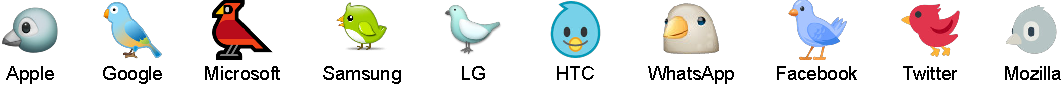
\includegraphics[width=\linewidth]{figures/emojipasswords/emoji-bird-comparison}
	\caption{
		\label{fig:emojipasswords:emoji-bird-comparison}
		Although the ``bird'' emoji is encoded with the same unicode character (U+1F426), its visual representation differs strongly across platforms and vendors.
	}
\end{figure}

%QUESTIONS
In this chapter we would like to explore pragmatic and hedonic qualities of emoji-passwords. We aim to answer the following research questions:
\begin{itemize}
	\item[RQ1] Do emojis in passwords help users create more \textbf{memorable} passwords?
	\item[RQ2] How do platform-dependent renderings (\textbf{fragmentation}) affect memorability?
	\item[RQ3] What is the most feasible \textbf{user interface} to enter emoji-passwords?
	\item[RQ4] What are users' password \textbf{selection strategies} and behaviors?
	\item[RQ5] What are users' general \textbf{attitudes} towards using emojis inside passwords?
\end{itemize}

This chapter reports on a mixed-method experiment carried out to investigate the usability of alphanumeric passwords that contain emojis. Beside myself, Florian Mathis and Heinrich Hussmann made contributions to the project. The results have been previously published at OzCHI 2017 \cite{Seitz2017Emojipasswords}. In the following, we put the design space for emoji-passwords into context, describe an empirical research study, and derive implications on the effective use of emoji-passwords.

\section{Background and Context}
\subsection{Emojis}
%definition and history / origin
Literally translated from Japanese, emojis\footnote{The plural form for ``emoji'' is both ``emoji'' (Japanese) and ``emojis'' (adopted to English). For clarity reasons the chapter sticks to ``emoji\textbf{s}''.} are ``picture words'' \cite{Taggart2015NewWords}. They are primarily used in mobile messaging applications like WhatsApp, iMessage, and alike, to express emotions and add subtext in messages. Before emojis arrived, this has been possible with \textit{emoticons}, i.e. combinations of regular characters that convey emotions like \texttt{:-)} \texttt{<3} and \texttt{:-O}. However, emojis are visually richer and much more versatile. The current version of the Unicode standard lists around 2800 emojis (see footnote \ref{foot:full-list-of-emojis}) categorized by topics, and roughly 150 are added each year. In 2015, emojis saw a stark increase in usage numbers. Both iOS and Android added special software keyboards that allowed users to easily enter emojis through direct touch input. %This contributed to the addition of emojis in half the image-captions on Instagram\footurl{https://engineering.instagram.com/emojineering-part-1-machine-learning-for-
emoji-trendsmachine-learning-for-emoji-trends-7f5f9cb979ad}{10.03.2018}. 
Often, users replace entire words or blocks of text with emojis. Although emojis are useful to cross language barriers, their meaning is not always clear \cite{Miller2015BlissfullyHappyEmoji,Tigwell2016EmojiMisunderstandings}. Researchers have started to investigate misinterpretation in many ways, and have proposed solutions like a ``disambiguation API'' \cite{Wijeratne2010}. 

\subsection{Emojis in Authentication}
% visual authentication
The growing adoption rates of emojis in various application areas has not gone unnoticed by the \gls{USEC} community, who started trying to improve authentication schemes with emojis. One of the first solutions was presented by Intelligent Environments\footurl{https://www.intelligentenvironments.com/now-you-can-log-into-your-bank-using-emoji/}{10.03.2018}. Their \textit{emoji-passcode} system would allow customers to select four emojis from a 9x5 grid to log into mobile banking apps. However, the concept has not been widely adopted. Golla \etal, respectively Kraus \etal, proposed a similar system that was targeted at screen-locks for mobiles \cite{Golla2017EmojiAuth, Kraus2017Emoji}. In essence, their EmojiAuth system replaces each digit on a PIN-pad with an emoji. In two user studies, they evaluated the concept and showed that both security and usability of unlock mechanisms can be improved this way. On the other hand, we were able to find only one publication about using emojis as part of an alphanumeric password  \cite{AlHusainy2015EmojiPasswords}. Al-Husainy and Mali focused on user-account passwords on desktop computers but did not present an empirical evaluation of the concept. We believe web pages and mobile applications are the primary use case for emoji-based authentication. This application area is still underexplored. 

\subsection{Opportunities}
The combination of emojis and alphanumeric characters generates a wide range of research questions, and we can only answer a small subset of them. In particular, we explore password selection strategies that may hint at potentially risky behavior. It is likely that emoji-passwords share some traits of alphanumeric passwords. For instance, the topology of a password is an important metric to gauge its guessability. Therefore, we would expect to observe some topologies reported by Weir \etal  \cite{Weir2010MetricsPolicies}, Ur \etal \cite{Ur2015PWCreationLab}, and Kuo \etal \cite{Kuo2006HumanSelectionMnemonic}. The latter indicated that some users had already used emoticons inside passwords in 2005. Although we cannot realistically measure guessability of emoji-passwords at this time, we can explore emerging patterns. For instance, we can elicit where users put their emoji and how they choose it. Emoji-passwords are a hybrid between knowledge- and recognition-based authentication, so they demand effort from both the lexical and visual memory \cite{Renaud2009VisualSnakeOil}. Therefore, this approach could turn out to be either a memorability advantage or disadvantage. Since the answer to this question is very open, we refrain from generating hypotheses altogether.

%TODO: this paragraph does not make tooooo much sense, but is intended to show a) many unanswered questions, b) what we expect to find (but that's not enough to form hypotheses), c) that we can already discover patterns that serve modelling password strength/weaknesses.

%Finding the right emoji:
%\cite{Pohl2017BeyondTextEmoji} input problems
%Other use of emojis in research: 
%\cite{Marengo2017EmojiPersonality} using emoijs as indicators for personality
%\cite{Lorenzi2017Emojitcha} using emojis as captchas

\section{User Study}
% GOALS
The goal of our project was to understand the human factors and usability constraints of emoji-passwords, which can be used to evaluate the idea of empowering users as persuasive strategy. To achieve this goal, we created a prototype that allowed entering emojis inside password-fields and evaluated it with a mixed-methods user study to cover a larger spectrum of opportunities and caveats. The first part took place in a controlled lab environment, while the second was carried out remotely without moderation. To explore different dimensions of usability and to follow common practice, password selection and recall were spread out across different days. In the following we describe the prototype, procedure of the two methods, the corresponding variables, and sample of our study. 

% overview + motivation to use mixed methods.
\subsection{Prototype}
\begin{figure}
	\centering
	\begin{subfigure}[t]{0.49\textwidth}
		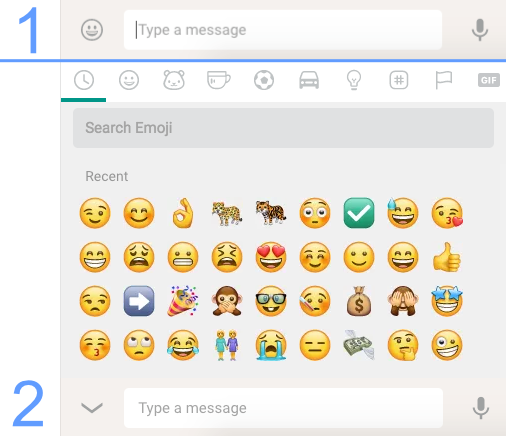
\includegraphics[width=\textwidth]{emojipasswords/whatsapp-picker-steps}
		\caption{\label{fig:emojipasswords:whatsapp-point-and-click}Two-step point-and-click interface  in WhatsApp.}
	\end{subfigure}
	\begin{subfigure}[t]{0.49\textwidth}
		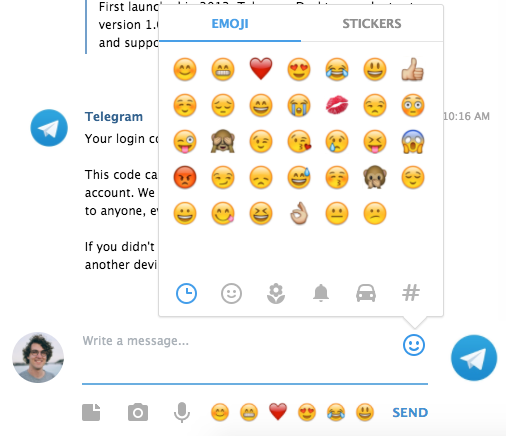
\includegraphics[width=\textwidth]{emojipasswords/telegram-picker}
		\caption{\label{fig:emojipasswords:telegram-point-and-click} Telegram shows the picker after the user hovers  the emoji button. Moreover, recently used emojis are shown beneath the text-field.}
	\end{subfigure}
	
	\caption{\label{fig:emojipasswords:real-world-pickers}
		Examples for point-and-click interfaces (``emoji picker''). \textit{Progressive disclosure} is used to access
		the list of available emojis: The user first needs to interact with a control element (emoji button) or start typing a special character (mostly ``:''), before an emoji can be selected by clicking or auto-completion of the shortcode. The emoji is then inserted into the text field.
	} 
\end{figure}
% general ways to do this.
% web-based
The project focused on using emoji-passwords on web sites, therefore we built a web-based prototype with standard technologies (PHP, HTML5, JavaScript). We identified two solutions to enter emojis on a desktop computer: via a point-and-click interface, and ``shortcodes''. Most web-versions of messenger applications, e.g. WhatsApp Web, Telegram Web, Hangouts, etc., use the point-and-click approach (see Figure \ref{fig:emojipasswords:real-world-pickers}). A few communication tools also allow entering a predefined word that is then translated into an emoji. This \textit{shortcode} often needs to be put into braces, e.g. (smile) on Skype, or stand between two colons, e.g. :smile: on Slack (see Figure \ref{fig:emojipasswords:slack-emoji-interaction}). We implemented a prototype based on point-and-click selection and Slack-style shortcodes. However, shortcodes were not auto-completed, which is generally discouraged for passwords \cite{Melicher2016UsabilityMobileTextPasswords} and there was no ``recent emoji'' feature. 
% passwords show in clear text below the input field to verify their selection.
After clicking an emoji, the prototype did not use the unicode character inside the password field for technical reasons\footnote{emojis typically break the masking of password fields, because their encoding differs in byte-size}. Instead, the shortcode was automatically inserted and masked. To allow checking the entered password, it was displayed in plain text beneath the input fields (see Figure \ref{fig:emojipasswords:policy-memo-instruction}). 

% reduced set of 50 emoji.
While unicode v11.0 contained 2789 emojis\footnote{\label{foot:full-list-of-emojis}\url{https://unicode.org/emoji/charts/full-emoji-list.html}\la{08.03.2018}}, we reduced the number of available emojis to 50 for several reasons. First, we found through iterative testing that there was a selection bias, if the full range of emojis was offered; testers mostly included emojis from the first page. %While selection bias could be mitigated through randomization, usability would strongly suffer if the user had to identify a particular emoji among 2800 emojis in random order. 
Second, Golla \etal used a similar approach for their EmojiAuth system \cite{Golla2017EmojiAuth, Kraus2017Emoji}. Last, reducing the number very likely facilitates recognition and potentially increases the memorability of the emoji-password.

% available emojis: 14 people and smileys, 7 nature and animals, 6 foods, 5 activity, 6 objects, 7 symbols.
The 50 emojis were selected with certain features in mind. To evaluate issues arising from similarity, around a third of emojis should mutually resemble each other. Fragmentation issues during authentication can only be seen for emojis whose appearance strongly differs on other platforms. Moreover, the emojis should appeal to users, e.g. because they are familiar with them. To achieve this, different emoji-categories should be considered. We identified 50 suitable candidates from the most-used\footurl{http://emojitracker.com/}{08.06.2018} emojis on Twitter from multiple categories: \textit{smileys \& people} (14), \textit{animals \& nature} (7), \textit{food and drink} (6), \textit{activities} (5), \textit{objects} (6), and \textit{symbols (7)}. We opted to include more smileys, because this roughly 50\% of unicode emoji characters fall into this category. Our emoji-picker randomly arranged the emojis in a 10x5 grid to isolate selection-by-position effects. 

% emojis: iOS 9.3, b/c WhatsApp used these on all platforms at the time (most commonly used messenger app in DE)
The prototype allowed to switch between two versions of emojis. The default version was based on the emojis from iOS 9.3 (see Figure \ref{fig:emojipasswords:ui-open-picker}). This default was chosen, because WhatsApp used the same emoji-style across all platforms at the time of the study. Thus, we could expect participants to be familiar with them. The second style was based on Android 7.0 (``blob emojis''\footurl{https://medium.com/google-design/redesigning-android-emoji-cb22e3b51cc6}{08.03.2018}). 

\begin{figure}
	\centering
	\begin{subfigure}[t]{0.49\textwidth}
	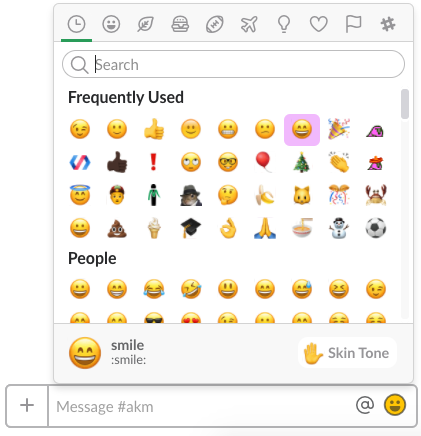
\includegraphics[width=\textwidth]{emojipasswords/slack-picker-shortcode}
	\caption{\label{fig:emojipasswords:slack-picker} The picker shows the short-code of the emoji for future use.}
	\end{subfigure}
	\begin{subfigure}[t]{0.49\textwidth}
	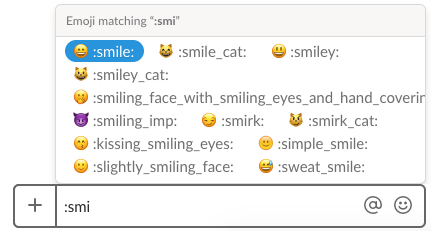
\includegraphics[width=\textwidth]{emojipasswords/slack-shortcode-auto}
	\caption{\label{fig:emojipasswords:slack-picker-shortcode} The user can guess the shortcode. Slack offers matching emojis.}
	\end{subfigure}
	\caption{\label{fig:emojipasswords:slack-emoji-interaction}
		Slack allows the user to utilize both a point-and-click interface and shortcodes to enter emoijs.
	} 
\end{figure}


\subsection{Password Selection in the Lab}
For the first part, participants were invited to a lab at the media informatics research group. The primary task was to create a password that participants could remember well. There was no independent variable for the password selection task, thus participants all received the same study instructions. 

\subsubsection{Metrics}
% no clear-text passwords, emojis and zxcvbn stats, hashes are stored for verification purposes.
We logged the chosen emojis and their positions inside the passwords. Moreover, we analyzed password characteristics with zxcvbn and stored this to the database along with the hashed password. 
% time
As an indicator for usability of either the picker or the shortcodes, we measured the time taken to select the password. Here, we used the ``focus'' and ``blur'' events as start and end points. 

% self-reported: (questionnaire) selection strategies, motivation, input type (motivation, ease of use, usefulness, 5 point scale)
On the qualitative side, we used ordinal five-point scales to collect attitudinal data about using emojis inside passwords, the picker, and shortcodes. Demographic data and self-reported password behavior helped us put measurements into context. 
% think aloud protocol, exit interview.
Everything that participants said during the study was protocolled. 

\subsubsection{Procedure}
% PC self guided with aid of experimenter
% briefing and informed consent (log data will be generated from interactions).
After an in-depth briefing on the purpose of the study and data collection practices, an experimenter explained each step of the study. We provided a standard desktop PC to complete the tasks, which were mostly self-guided. First, participants created a user ID. 
% create user Id (algorithm first letter parents' namses, birthplace, birth month)
Since they were going to need this ID later on to allow us matching the lab and field data, we provided a simple algorithm to create an ID. Participants were asked to take the first letter of both their parents' first names and their own birth place, appended by the digit of their birth month (e.g. ``IKP10''). This algorithm, albeit not perfectly random, was sufficient to protect \acrlong{PII}.

This was followed by a questionnaire on demographic data, password coping strategies and attitudes towards emojis in passwords, e.g. ``\textit{how likely would you consider using emojis in a password?}'' At this point of the study, participants had not yet created an emoji-password, so their attitudes were not biased by later tasks. 
% instruction: difference between emojis and emoticons (shared understanding)
We also briefed them about the difference between ``emojis'' and ``emoticons'' to avoid misinterpretation. 

% password selection & commitment (think aloud)
% scenario: whatsapp requires all users to secure their account with a password (basic8 + emoji, feedback provided when policy is met.) 
Afterwards, participants completed the password selection task using the prototype. A significant part of the screen was dedicated to list all emojis and their short codes. To provide sufficient background information and introduce a realistic risk \cite{Krol2016ExperimentDesign}, the task included a scenario. It asked participants to imagine that they had used WhatsApp for some time and now a new security precaution is introduced. As a safety measure, they were now required to prove their identity with a password upon activating WhatsApp on a new device. The password needed to consist of at least eight alphanumeric characters and at least one emoji. 
% repeat password, only proceed if confirmed to have memorized the password.
Participants then had to repeat the selected password, and tick a box to confirm that they had memorized it (see Figure \ref{fig:emojipasswords:policy-memo-instruction}). 
% usability rating (picker/short codes, emoij-password concept post experience)
This was followed-up through a reflective self-assessment of their behavior during the study (cf. \cite{Fahl2013EcologicalValidityPasswordStudy}), and a structured questionnaire on their selection strategies. 

% interpretation task 
The study concluded with an interpretation task of two given emojis, namely the ``information desk person'' (\emoji{1F481}) and ``folded hands'' (\emoji{1F64F}). Those were not available during password selection, and we intended to assess their suitability for future inclusion. In total, the whole session duration was below 15 minutes.

\begin{figure}
	\centering
	\begin{subfigure}[t]{0.49\textwidth}
		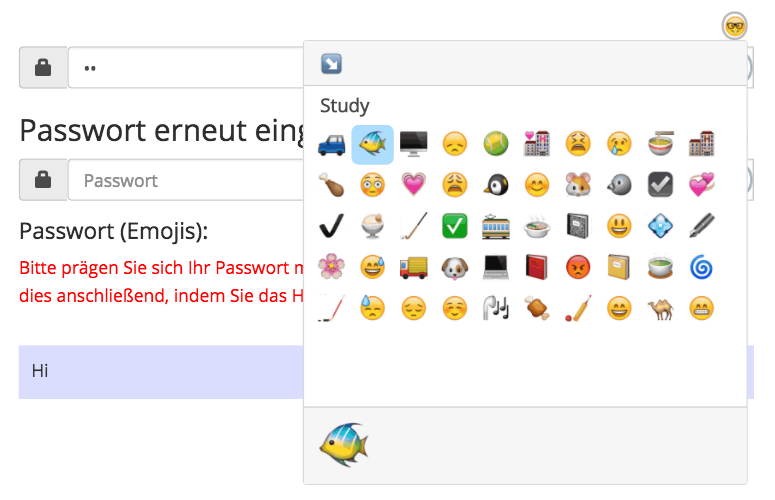
\includegraphics[width=\textwidth]{emojipasswords/open-picker}
		\caption{\label{fig:emojipasswords:ui-open-picker} Point and click interface. It is opened by clicking on the \emoji{1F913} button. The order of emojis is randomized. Upon selecting an emoji, it automatically closes.}
	\end{subfigure}
	\begin{subfigure}[t]{0.49\textwidth}
		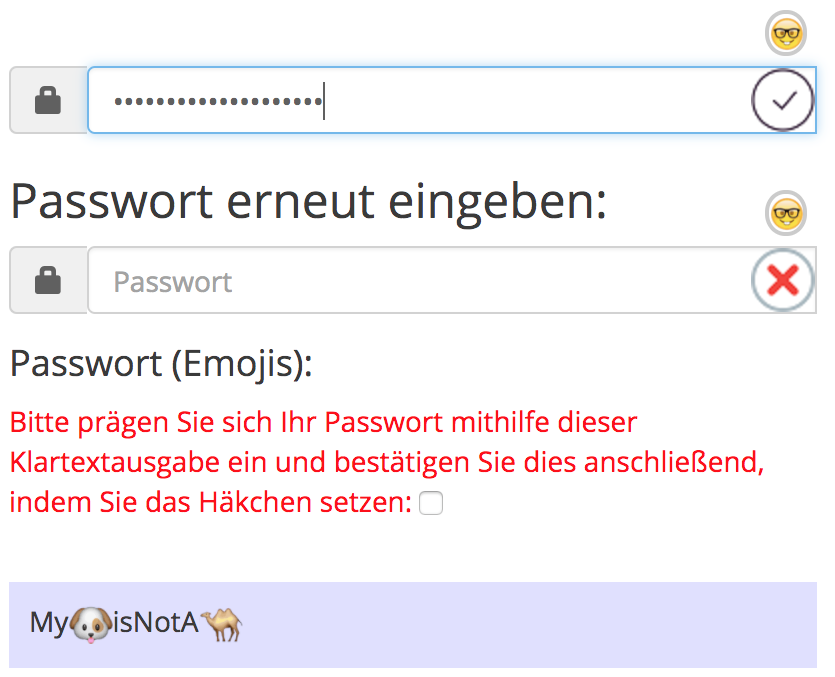
\includegraphics[width=\textwidth]{emojipasswords/ui-slim_cropped-2}
		\caption{\label{fig:emojipasswords:policy-memo-instruction} Screenshot of the user study. The selected password needed to be re-created. Additionally, participants need to tick a check-box to confirm that they had memorized their password.}
	\end{subfigure}
	\caption{\label{fig:emojipasswords:prototype} Prototype as used in the study.}
\end{figure}

% recall
\subsection{Unmoderated Remote Memorability Study}
% exactly one week after participant, invitation to return to the online study. 
Exactly one week after completing the first study part in the lab, participants were invited to return for the second round of tasks on-line. This primarily focused on memorability metrics and a reassessment of attitudes. 
\subsubsection{Independent Variable}
% emoji rendering (2 levels / degrees of freedom ): control group received iOS 9.3 (the same kind as in the lab), experimental group different treatment (Androd 7.0). 
To gauge the influence of emoji fragmentation, we used one independent variable \textit{``rendering''} with two levels. For the \textit{control} group, emojis in the picker were rendered as before. In the experimental group, we replaced the iOS emojis with the Android 7.0 version. No other variations were made. 
\subsubsection{Dependent Variables}
% attempts to log in (max 3). 1 = immediate success, no errors.
We measured the number of attempts participants needed to log in. If they failed to log in on the first try, we counted this as an error.  Moreover, we collected memorization and recall techniques. 
% qual: how memorized? attitudinal ratings, qualitative feedback on overall technique
Finally, subjective usability ratings on the overall concept and qualitative feedback were gathered. This part of the study took about five minutes.

\subsubsection{Procedure}
% randomly put into the two treatment groups, different participation link for the two groups via email
Participants were randomly assigned to one of the two experimental groups. We emailed the corresponding link to the online study and requested completion within two days. 
% recreate user id same algorithm as in the lab)
The web page instructed them to recreate their user ID, providing the same algorithm as in the first part. Afterwards, participants were asked to log-in via their previously selected password. After unsuccessful attempts, the log-in counted as failed and the study proceeded automatically. However, as a memory support tool, we displayed the list of short codes after the first failed attempts. The study concluded with an attitudinal questionnaire about the perceived usability of the concept. 

\subsection{Recruiting and Demography}
We spread a registration link for a ``study on emojis'' via social networks and an official university newsletter. A 5€ shopping voucher served as incentive. The study was announced to take around 15 minutes. 40 people were screened in and all showed up to their study appointment. All of them were students at the LMU, and aged between 19 and 44 ($M=23$).  %TODO add standard deviation. (if we have it)
Users in this age rage are most likely to use emojis on a regular basis \cite{EmogiResearch2016}. 39 participants returned for the second study part on-line. The control group was formed by 20 participants, and the experimental group by 19. 
%TODO maybe add hypotheses, but that's not super necessary
\section{Results}
In the following, we explain participants' sentiment regarding the usage of emoji-passwords before we report empirical observations and qualitative analyses. 
\subsection{Sentiment}
Sentiments were assessed with agreement levels to five-point scale items (1 = strongly disagree, 5 = strongly agree).
%before.
Before participants selected an emoji-password for the first time, they were already reserved towards the statement ``I would consider adding an emoji to a password'' ($M=2.7, SD = 1.4, Md=2$). They did not regard emojis as a way to make passwords more memorable, either ($M=2.8, SD = 1.3, Md=3$).
%after first trial
After completing the first part, the statement ``I liked adding an emoji to my password'' was rated slightly more positively with an average of 3.6 ($SD=1.19, Md=4$). 
%final sentiment.
Having fulfilled all tasks, participants saw general benefits to add emojis in passwords ($M=3.5, SD = 1.2, Md=4$). Eleven found the enforced emoji-policy annoying. Hence, attitudes towards using emojis for their personal passwords in the future were rather negative ($M=2.6, SD = 1.3, Md=2$), although they were slightly more positive about potential memorability benefits than before ($M=3.1, SD = 1.3, Md=3$). In summary, participants were reserved towards adopting emoji-passwords, but their sentiment covered the full spectrum. 

\subsection{Emoji Selection}
% quant:
% 	which emoijs were selected (distribution graph like on slides)
% 	position in password -> new graph (R!), with data from slides.
\subsubsection{Statistics}
Our 40 participants chose a total of 22 different emojis. Most commonly, participants chose the camel (:camel: \emoji{1F42B}, n=5), penguin (:penguin: \emoji{1F427}, n=5), grinning face (:grin: \emoji{1F601}, n=3), tea (:tea: \emoji{1F375}, n=3), dog (:dog: \emoji{1F436}, n=3), diamond (:diamond\_shape\_with\_a\_dot\_inside: \emoji{1F4A0}, n=3), and cherry blossom (:cherry\_blossom: \emoji{1F338}, n=3). The remaining 15 emojis were chosen less than three times each. Six users added two emojis to their password. On average, password fields had focus for 52.9 seconds ($SD = 55.00$).

\begin{figure}
	\centering
	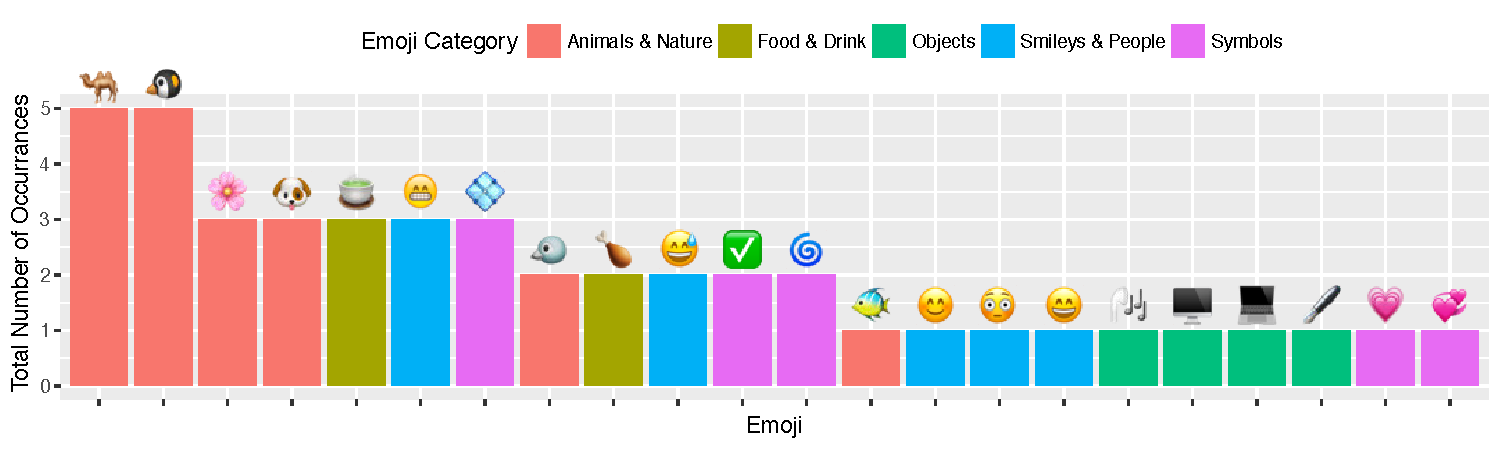
\includegraphics[width=\linewidth]{figures/emojipasswords/emoji-distribution-histogram}
	\caption{\label{fig:emojipasswords:distribution-histogram} Histogram of the chosen emojis and their categories. Patterns emerge already in our sample with 40 participants, which hints at potential security problems.}
\end{figure}


Before passwords were hashed, we determined the position of the emojis. The majority of participants who only selected one emoji put it at the end ($n=19$), while seven started with it and eight put it somewhere in the middle. Adding the emoji there is the most cumbersome approach due to the double modality switch between mouse and keyboard if the picker is used. The six participants who picked two emojis either put both at the start ($n=1$), as the first and last characters ($n=2$), only in the middle as two consecutive characters ($n=1$), or as middle and last character ($n=2$). Figure \ref{fig:emojipasswords:position-histogram-by-strategy} shows a detailed breakdown of the chosen positions. 
\begin{figure}
	\centering
	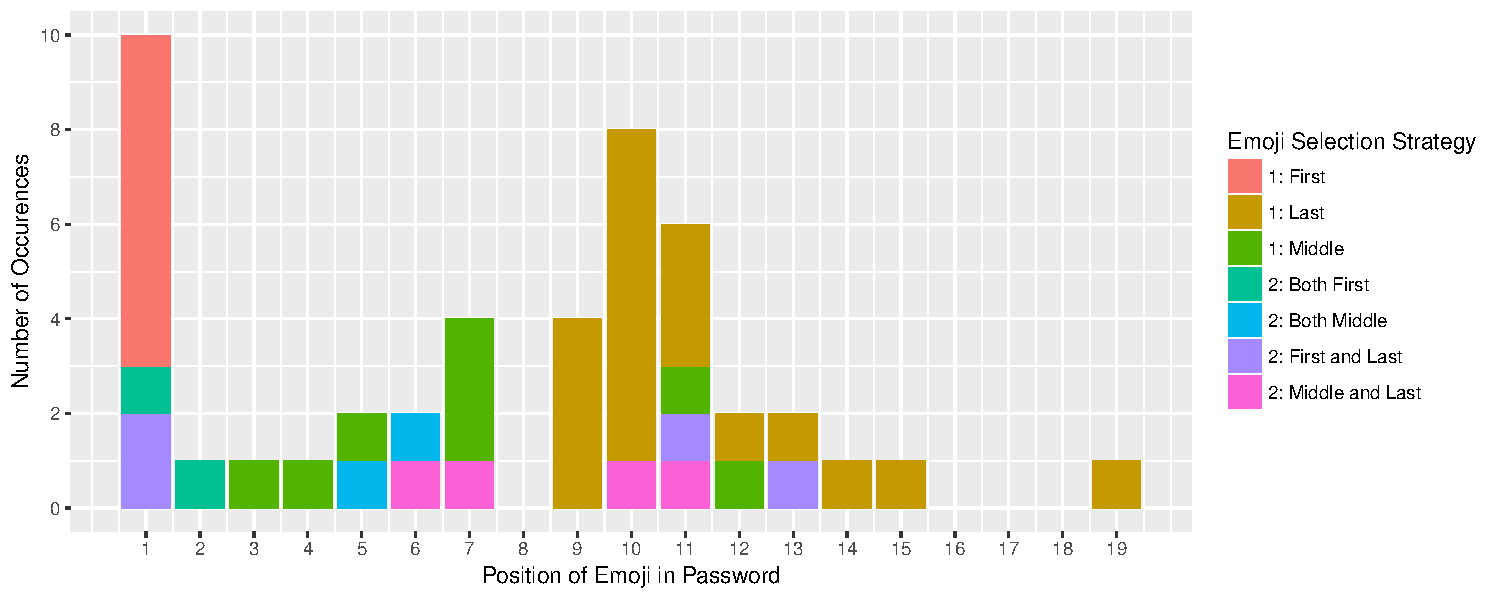
\includegraphics[width=\linewidth]{emojipasswords/position-histogram-by-strategy}
	\caption{\label{fig:emojipasswords:position-histogram-by-strategy} Histogram of absolute positions of emojis inside passwords. The prefix (1:, 2:) denotes the total number of emojis in the corresponding password. Most participants either started or finished their password with the emoji.}
\end{figure}


\subsubsection{Self-Reported Selection Strategies}
Except for the emoji, our participants mostly claimed to have created a password like they normally would ($M=3.4, SD=1.45, Md=4$). 
% 	selection strategies
We elicited selection strategies in two ways: a list of probable strategies that we identified in pre-tests, and an open question where participants were asked to describe their method in detail. Half of the participants indicated that they used an emoji that fits the alphanumeric part of the password. Four said that they preferred an emoji that they frequently use, while another four randomly chose an emoji. The remaining participants either associated the picture to a life event ($n=3$) or hobby ($n=1$). Eight participants elaborated on their tactics in high detail, and their strategies were more individual than the predefined categories. 

Through collaborative thematic analysis, a method similar to affinity diagramming, we identified themes in all qualitative statements and the think-aloud protocol. After the first round of coding, there were 42 codes that were further reduced in an axial coding step. The resulting overall themes were:
\begin{itemize}[leftmargin=*]
	\item \textbf{Internal consistency:} The emoji semantically matches the alphanumeric part of the password, e.g. putting a camel emoji \emoji{1F42B} after the Greek word for ``heat'' (P26). 
	\item \textbf{Context cues:} The password contains a hint to the participant's location or to its purpose. For instance, participants used the computer emoji \emoji{1F5A5} because they created the password on a PC (P34). Another participant picked the check mark \emoji{2705} because it stands for \textit{completing} the study (P38). 
	\item \textbf{Replacement:} The emoji replaces either a letter or an entire word. For instance, P17 replaced the letter ``p'' in their password with a penguin \emoji{1F427} because both \textit{words} begin with the same letter.
	\item \textbf{Appeal:} The emoji visually or emotionally appealed to the participants (mentioned twice for the flower emoji \emoji{1F338})
	\item \textbf{Liking:} Participants had an affection or personal connection to the emoji, e.g. penguins \emoji{1F427}.
	\item \textbf{Usability and Security:} An emoji that serves to increase usability or security of the password. Usability could be improved either with a particularly easy-to-type shortcode (:grin:), or by choosing an emoji that ``stand out from the rest, because they look too similar'' (P32, chose the penguin). Security was achieved through perceived randomness or unpredictability (mentioned twice for the diamond \emoji{1F4A0}).
\end{itemize}

From those six themes, we can see a common story line: The selection strategies can be read as an attempt to \textbf{improve memorability} of the password. Most participants intuitively focused on creating a password that they could recall. None of them mentioned the option to write them down or store passwords externally. The selected emojis thus matched individual memorization approaches.

\subsection{Input Methods}
% quant: 
% 	how many used what
The majority ($n=32$) intuitively turned to the point-and-click interface to enter their emoji. Five participants used the short-codes and three tried both modalities. Both the picker and the short codes received positive usability ratings from the respective participants ($M_{picker})=3.8, SD_{picker}=1.1, M_{short}=4.2, SD_{short}=1.3$),  Thus, it was easy for participants to enter emojis on a desktop computer in both modalities. Interestingly, the three participants who tried both methods started with the picker and then continued to use the short codes, because they found it more convenient.

% qual:
%	why? feedback, sentiment.
Through a qualitative analysis of the think aloud protocol we found that participants considered both advantages and disadvantages of both moth methods. The picker was perceived as easy and fast to use, while being less prone to typing errors. Often, participants mentioned that they were already familiar with this entry method (e.g. from WhatsApp web), so they did not have to learn anything new. On the other hand, they described the progressive disclosure paradigm as potential problem, because the button that triggers the picker could be overlooked. Also, some mentioned that it is cumbersome to switch between mouse and keyboard. Those who used the shortcodes appreciated the speed of entry and low effort to add the emoji to the password. However, learning and memorizing the corresponding codes were seen as the main drawbacks. The sentiments did not significantly change in the second part of the study ($M=3.5, SD=1.2, Md=4$, overall happiness ratings). In summary, we can conclude that participants made an active choice about the chosen input method and they were happy with their choice. %TODO add likert plot.

\subsection{Memorability and Recognition}
% quant: 
%	how many succeeded? which emojis were involved in errors? group differences
% 	show the differences visually (like google talk)
\subsubsection{Success Rates}
Login success rates in the second session did not significantly differ between the two study groups. In the control group, who saw the identical emoji set, five participants failed to log in after a week and 15 succeeded. The experimental group, who received the Android version of the emojis, counted six log-in failures, while 13 participants were able to authenticate despite the change of rendering. This difference was not statistically significant ($\chi^2(1)=0.21, p>0.5$). From those who succeeded, 12 participants authenticated on the first try in the control group, whereas this was slightly lower in the experimental group ($n=8$). Again, the change was not statistically significant ($\chi^2(1)=1.25, p>0.1$), which is probably owed to the sample size. The medians of failed attempts, which are potentially more descriptive in this situation, did differ: the control group's median was 0, while it was 1 in the experimental group. Figure \ref{fig:emojipasswords:success-vs-failures} visualizes successful and unsuccessful login attempts in high detail. There, we can trace back the emoji that were included in incorrectly entered passwords. Success and failure rates in the ``Animals \& Nature'' category balanced in both groups. However, participants were twice as likely to fail in the experimental group, if their password contained an emoji from the ``Smileys \& People'' category. Figure \ref{fig:emojipasswords:experimental-group-failures} shows that emojis differing strongly from the iOS version were more associated with login failures. ``Symbols'' were the category with the highest failure rate across both groups.


\begin{figure}
	\centering
	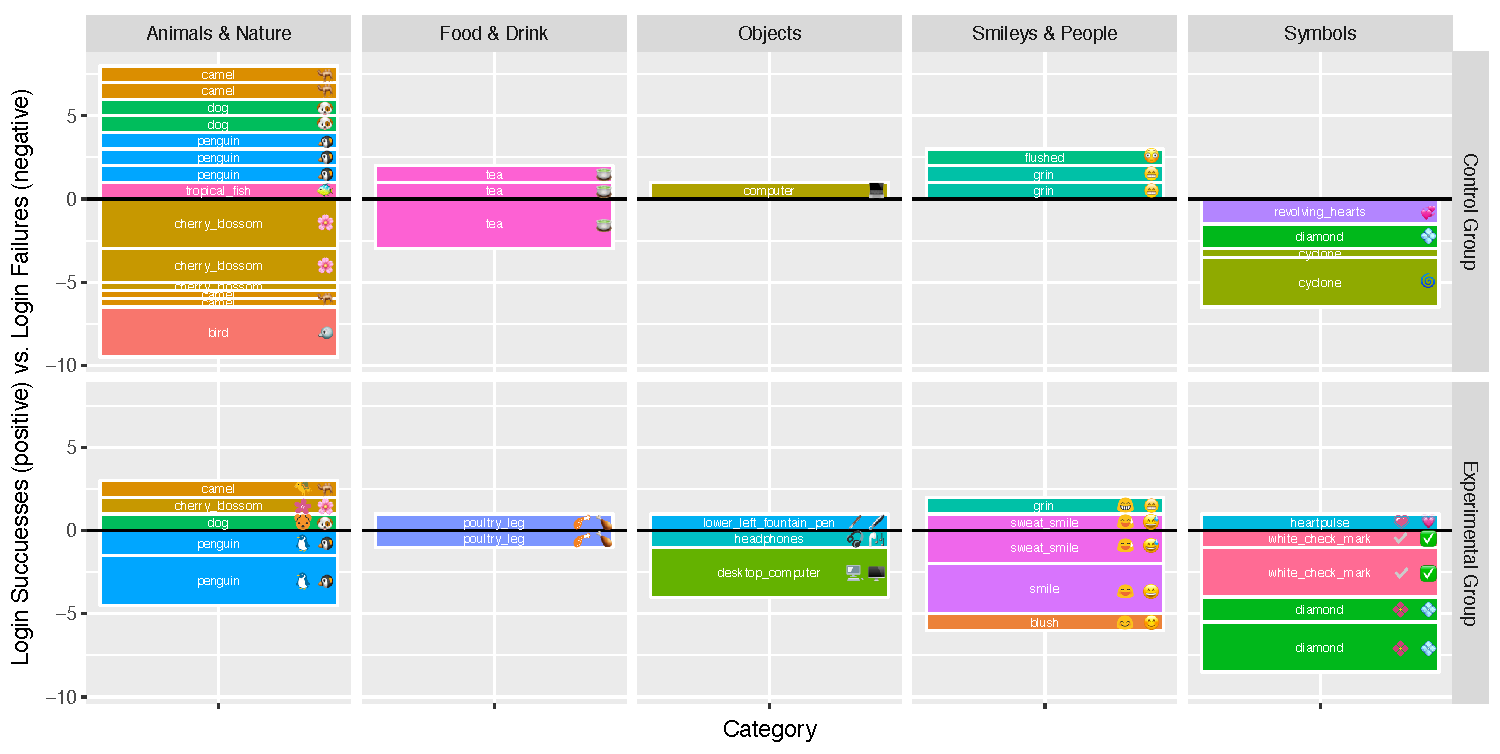
\includegraphics[width=\linewidth]{figures/emojipasswords/success-vs-failures}
	\caption{
		\label{fig:emojipasswords:success-vs-failures}
		Detailed overview of the emojis inside passwords, stacked to immediately successful logins (y-positive) and error-prone login attempts (y-negative)
	}
\end{figure}

\begin{figure}
	\centering
	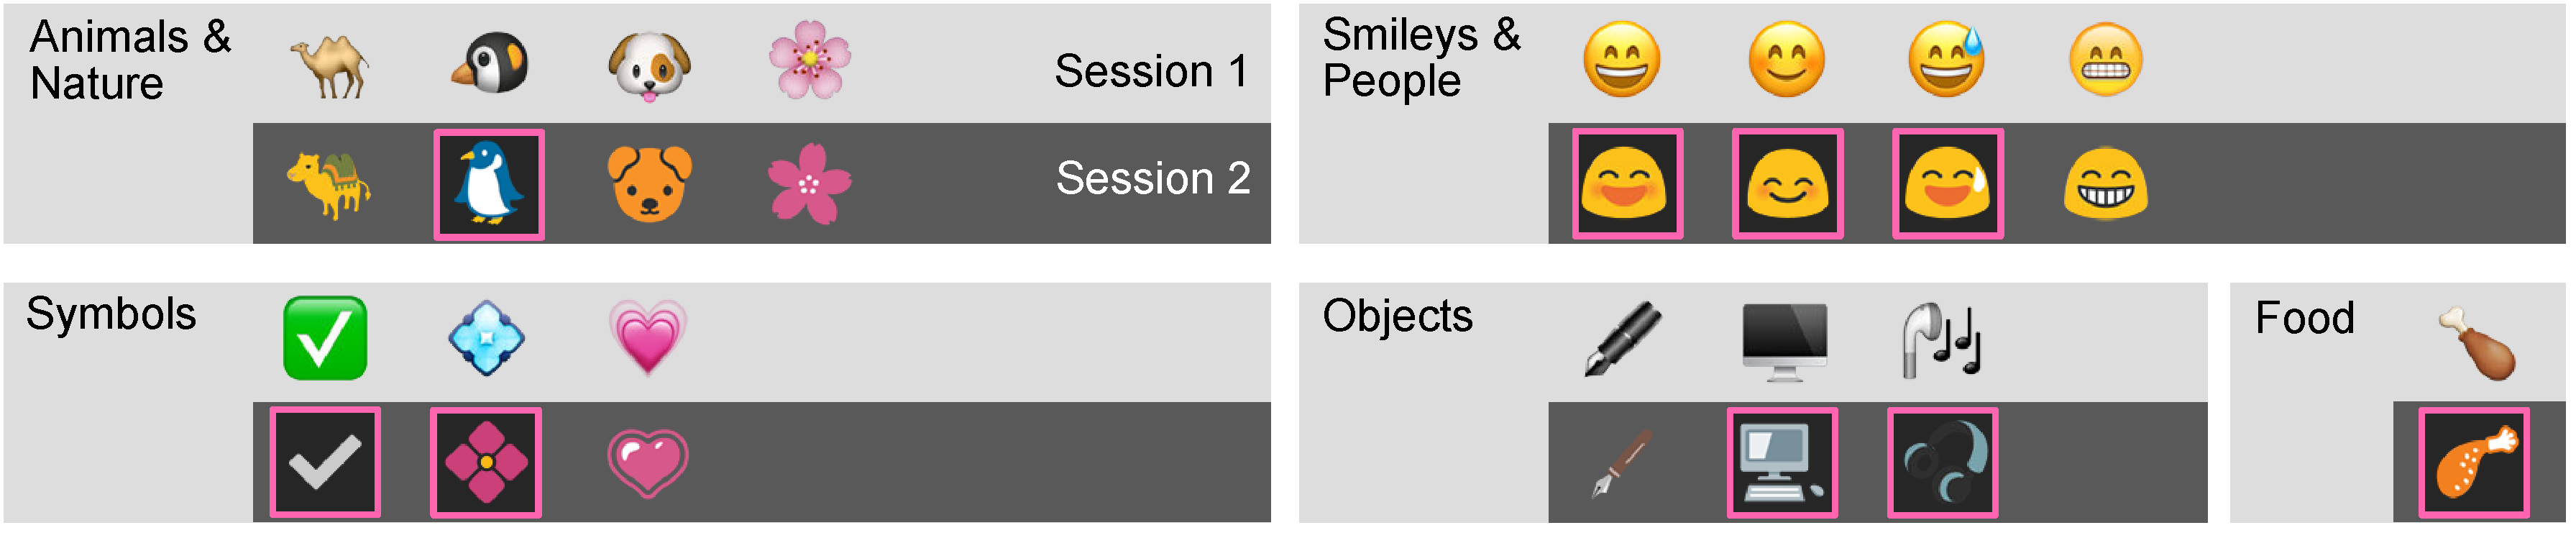
\includegraphics[width=\linewidth]{figures/emojipasswords/experimental-group-errors}
	\caption{
		\label{fig:emojipasswords:experimental-group-failures}
		Chosen emojis by the experimental group. The ones that were part of failed login attempts are highlighted with a dark box. It is these that differ strongly from the iOS version from session 1, which is evidence for the usability problems caused by fragmentation.
	}
\end{figure}


\subsubsection{Textual Feedback}
%	noticed differences?
To assess the influence of the rendering modification, we asked whether participants had noticed any differences in the appearance of the emoji. Although the emojis remained identical in the control group, 7 out of the 20 participants indicated that they had noticed a change. This is hard to interpret, but assume that they meant the order of the emoji inside the 10x5 grid. In the experimental group, where emojis did in fact \textit{look} different, 16 out of 19 participants (84\%) talked about this change in the response field. Eight of them did not perceive the alteration as troublesome, while another eight felt that identifying the right emoji was challenging. For three participants, the change of emoji-type was insurmountable: One participant was very sure to have selected the correct emoji, because she picked a ``happy face'' to express herself. However, she reported to have failed because she was unable to pick the correct emoji in the second study session. Another participant, who successfully authenticated with his emojipassword, indicated that he could only find the right emoji after a Google search. Finally, one participant mentioned that he was troubled by the different versions of the check mark, so he used a trial and error approach until he succeeded.

\subsection{Memorization Techniques}
%	how did people remember? memorization strategies
%	was the short code useful?
The emoji-picker and the number of emojis was helpful to recognize and recall the password for 18 participants. The short codes did not achieve this, because only one person reportedly used the code as a cue to the password. A priori agreement levels to the statement ``Using emojis in a password makes it more memorable'' were neutral-low ($M=2.8, SD=1.4, Md=2$). In the exit survey, we again probed this sentiment and noticed a small, but statistically non-significant upward trend ($M=3.1, SD=1.3, Md=3$). 

\subsection{Interpretation Task}
% basically what we wrote in the paper to illustrate that already for two given emojis there is a huge range of possible interpretations.
The final task in the lab-session was to provide two word associations for two emojis (\emoji{1F481}, \emoji{1F64F}). Thematic analyses showed a wide range of themes for the ``service person'' emoji. A total of 14 distinct themes were visible, each mentioned by at least two participants. Most often, this emoji was associated with ``female'' ($n=6$) and ``pointing'' ($n=5$). The emoji depicts a bell-hop's ``tipping gesture'', which was interpreted as ``sassy'' ($n=2$) or ``bossy'' ($n=4$), too. Regarding the ``praying hands'' emoji, participants reached higher consensus on its meaning. Seven themes emerged from the word associations. Most commonly, the participants mentioned ``pray'' ($n=19$) and ``beg'' ($n=9$). These anecdotal examples highlight the problems produced by unclear meanings of emojis. For passwords, on the other hand, a bigger range of interpretations opens up more opportunities to create a story with emojis.

\subsection{Limitations}
% small sample size, homogeneous --> primary user group who are most likely to adopt emojipws as first-movers.
The results presented above need to be interpreted in the light of a few important limitations. First, the \textbf{sample size} was not large enough to bring about statistically significant test results. Naturally, the nullhypotheses (e.g. fragmentation does not affect recall) could be true, but with 40 participants, we lack statistical power to draw conclusive inferences, especially with a frequentist approach (which emoji was chosen \textit{how often}). Nevertheless, we saw emerging patterns that can be followed up with a quantitative user study. Our primary goal was the exploration of fragmentation and input issues, as well as attitudes. For this, the participants fell into the user group who would be most likely to try out emoji-passwords. This makes us confident the trends at least point into the right direction. To explore additional dimensions of the problem space around emoji-passwords, considering a more diverse sample is going to be useful in the future.

% ecological validity, self-report, novelty effects --> concrete plausible scenario, no reason not to trust P's.
Moreover, much of the elicited data is attitudinal, potentially affecting ecological validity of the study. However, we tried to mitigate issues by providing a realistic scenario and had them gauge their behavior. Here, most claimed they acted like they normally would, which has been shown to be a useful indicator as to the trustworthiness of the data \cite{Fahl2013EcologicalValidityPasswordStudy}. Nonetheless, emoji-passwords constituted an unfamiliar paradigm for all participants, despite their familiarity with both emojis and passwords separately. Therefore, novelty effects are possible in that participants might have spent more time to explore the possibilities than they normally would. However, subjective usability assessments on the feasibility of emoji-passwords were reserved. This indicates that respondents critically balanced the pros and cons and did not only focus on the benefits.

% no attack vectors, only usability, behavioral, attitudinal data --> future work, but maybe compare to the advantage of adding a Xclass requirement over X-1class requirement from another study. that should do. 

\section{Discussion}
In the following the results are put into context. We derive data-driven assessments about the feasibility of emoji-passwords. 
\subsection{Selection Strategies and Their Implications}
% what did they focus on? --> memorability, not security
% what does that mean?
% does that help?
% covariate: personality? \cite{Marengo2017EmojiPersonality}
% central point: focus on memorability, not security.
It was evident that participants were keen on creating a \textbf{memorable password}. So although people were enabled select a richer and more diverse password, we observed well-known reactions. 
% selection strategies are just like they used to be, i.e. bad.
The selection strategies were a direct translation of their usual patterns. Many of them noted that they were able to easily include emojis in their long-established strategies and coping behavior. As a consequence, we observed predictable patterns in selection strategies leading to simple attack vectors: participants favored items that helped them stick to their past selection strategies, which can be used to simply adapt existing cracking techniques.
% what does that mean? all bad?
We can read this as a bad sign, because emojis do not appear to break existing behavior, and only increase the theoretical space of creation strategies. At this point it is difficult to gauge practical security advantages entailed by enlarging the character set. Learning from past roll-outs of new authentication schemes, password \textit{strength} is unlikely to increase drastically by the use of emojis. 
% it's not going to get worse, security wise. so we got that going for us.
On the other hand, user-selected passwords have always shown predictable patterns and adding emojis probably will not aggravate the situation further. Therefore, the only major advantage of allowing users to pick emoji-passwords can be an improvement in how password authentication is perceived. In other words, it might help the \textbf{\gls{UX}}. Our data is helpful to identify the pitfalls that need to be considered to achieve good UX of emoji-passwords. 

\subsection{Factors in Good UX of Emoji Passwords}
% freedom to choose. not everyone likes that. large spectrum of ratings, median: neutral!
\paragraph{Freedom to choose} Good UX starts with respect and empathy. Users should not be forced to use emojis in their passwords. Our data discourages the use of a policy that mandates emojis, which a quarter of participants found annoying. From our first study on personality factors in attitudes towards policies we know that the spectrum in which users think about policies is large (cf. Section \ref{sec:personality:study-1}). Therefore, we argue in favor of autonomy and leaving it up to users to decide whether they want to use an emoji as part of their password(s). 

% IF users understand that they can use emoji-passwords, doing so needs to be frictionless and it is no problem to achieve this.
\paragraph{Learning Curve} Once users understand that they have the freedom to use emoji-passwords, the learning curve for this task looks fairly gentle. Our sample consisted of users who were already familiar with entering emojis on the desktop and therefore immediately knew what to do. Nonetheless, less experienced user groups should be offered enough help in case they decide to experiment with emoji-passwords. We also found that the short codes were mainly used by participants who aimed for efficiency. Thus, there is nothing wrong with allowing this interaction, but it should be most discoverable for a more advanced user group. 

%- don't have to learn anything new: emojis are familiar, interaction is familiar (shortcodes maybe for experts),

% rendering
\paragraph{Pragmatic Constraints for Passwords}\label{sec:emojipasswords:unique-constraints} 
%yo! stick to the same kind of emojis. be smart. whatsapp also has the same emojis on all platforms. but interference effects of using different platforms with different emoji-passwords are likely to arise. 

% fragmentation nono, consistency yes yes.
Although our sample came from a population of young adults who are highly experienced with emojis, some participants clearly struggled to identify the correct emoji after we exchanged the renderings. Therefore, inconsistencies across platforms could become a show-stopper. At the moment, there are a few problems that contribute to creating inconsistent experiences. 
% challenges: legal / copyright
First, although emojis standardized Unicode \textit{code-points}, vendors usually need to create custom emoji-\textit{pictures} for legal reasons. Sets under a public domain or nonrestrictive licenses do exist, but many vendors prefer providing on-brand experiences with a shared design language across products. It could thus be useful to form alliances like the \gls{W3C} to standardize graphical assets of emojis for password-fields. At the same time, software keyboards on mobiles need to match the password-emoji standard. As of now, emojis in built-in software keyboards do not necessarily match app-provided picker interfaces (see Figure \ref{fig:emojipasswords.app-vs-platform-emojis}). A simple solution to this inconsistency is to disable the built-in emoji-keyboard and let the app decide whether emojis are allowed.

% challenges: distinctiveness
After settling on a shared visual representation of emojis, it distinctiveness is another critical factor. Emojis within the offered set can generate troubles for users, if tuples exist that are very similar in their appearance. One of our participants mentioned this already in his selection strategy, because he was looking for an emoji that ``stands out'' and did not ``look like the others''. To avoid login failures from confusion, there needs to be a white list of emojis that only includes the highly distinctive ones. A candidate list based on geometric parameters like shape and color will then require evaluation through quantitative user research with a diverse sample.

% challenges: reduction?
A final challenge pertaining to the constraints of emoji-passwords are hard usability metrics like efficiency. UX benefits from a higher degree of freedom and creativity support are rendered futile if users need to browse through large lists of emojis only to find the correct item. Reducing the emoji-space to a subset emerges as useful approach that emerges to speed up recognition and efficiency. At the same time, it is conceivable that vendors stick to a limited, static subset that is randomly selected from the white-list of distinct emojis. Here, different sub-sets among vendors are potentially bearable because this mitigates password reuse. 

\begin{figure}
	\centering
	
\includegraphics[width=0.7\linewidth]{figures/emojipasswords/app-vs-platform-emojis}
	\caption{\label{fig:emojipasswords.app-vs-platform-emojis}
		Screenshots of entering emojis inside messages on WhatsApp. While the software provides a set of emojis that is consistent across all platforms supported by WhatsApp, users can still turn to the software keyboard built into their OS. In this case, the renderings, number, and order are inconsistent.
	}
\end{figure}



%\subsection{Similarity and Fragmentation Issues}
% not yet crystal clea

% from the paper: While three comments pointed towards a different interpretation, the numbers suggest that the different renderings of emojis did not have a notable impact on the login success rates, i.e. reproducibility of the emoji-passwords. The small sample size increases the likelihood of type-2 for statistical tests, though. In that case, this would explain the low voluntary readiness to include emojis in their personal passwords. Nonetheless, qualitative evidence is conclusive that users try to leverage emojis for creating more memorable secrets, if the emojis are required by the password policy.


%\subsection{Input UX}
% was it troubling? no
% does that mean, that all password fields on desktops should be accompanied by 
% of course entering an emojipw takes longer. even reading a text that includes emoji takes longer \cite{Gustafsson2017EmojiReadingTIme}


\section{Conclusion}
% summary and answers to research questions.
In this project, we empirically evaluated the usage of emojis in regular alphanumeric passwords. Our mixed-model user study with forty participants focused on attitudinal and usability aspects. From the selection behavior, memorability results and qualitative feedback we can conclude that emojis do not necessarily lead to memorable passwords (RQ1). Participants wanted to translate their usual password selection behavior to the new paradigm and tried to create memorable passwords (RQ4). When participants failed to log in, this could be partially traced back to fragmentation, i.e. differences in the visual representation of the same emoji characters (RQ2). Our sample population was experienced with emojis, but still struggled to match Android emojis to a previously selected iOS emoji. Their experience also allowed them to easily understand how to enter emoji-passwords on desktops through a graphical point-and-click interface (RQ3). Nevertheless, our prototype made potential issues salient for participants and thus their attitudes towards adopting emoji-passwords in the future were reserved (RQ5). 

% motivate / show the big picture of why our answers matter now. 
However, some vendors and service providers have enabled emoji support for passwords. For instance, Twitter\footurl{https://www.twitter.com}{10.03.2018} allows users to take advantage of this rich character set already now. The issues we explored in our study thus already affect a growing number of users, since solutions as to fragmentation and input UX do not exist at this point. However, more and more users are going to find out about the capabilities, perhaps because the feature is presented on blog- and news articles \cite{Dashinsky2015NoEmojisInPWs}. Therefore, the HCI community should act quick to create a better authentication experience to \textbf{scale solutions before problems are going to scale}. 
% lets stay realistic.
Realistically, the propositions and requirements discussed in Section \ref{sec:emojipasswords:unique-constraints} would require intensive negotiation based with much more user testing data.  It is unclear whether vendors are willing to make this investment. We argue that a standardized \textit{emoji-password-picker} with a random sub-set of white-listed, distinctive emojis is a desirable goal. The ``longer term solutions'' that are part of the Unicode standard (see Footnote \ref{foot:emoji-standard}) embrace ``embedded graphics'', which paves the way to mitigate fragmentation issues. Since primary tech companies have worked together on the standardization of emojis in the past, it would be fruitful to collaborate on authentication issues of emojis, too.

\paragraph{Future Work}
% focus on ux
Our prototype had not delivered the best possible user experience. This was partially owed to isolate confounding factors, e.g. a finished solution would not shuffle the order of emojis. Future studies on emoji-passwords need to intensely study different dimensions of user experience issues and potentials. To better understand the current state of emoji-passwords, a diary study might be worthwhile. It would be possible to answer interesting questions on how this novel kind of authentication influences well-established coping strategies. For instance, is it possible to \textbf{write down emoji-passwords}, and \textbf{share} them with somebody else? Can \textbf{password managers} already handle them?  Do users take more care to protect emoji-passwords from \textbf{shoulder surfers}? Such questions can help judge the feasibility of this approach and identify important pain points.

% quantify security beneftis and provide solutions. 
At the same time, we saw traditional patterns that might lead to weak emoji-passwords. Therefore, as a next step, the security benefits should be quantified. Perhaps, this is relatively easy to do with an \gls{mTurk} study. If our hunch about weak selection strategies is confirmed, it is clear that we need more data on the effectiveness of proactive strength feedback. Real-time password meters, particularly those based on zxcvbn, are currently unable to realistically gauge the strength of emoji-passwords. Therefore, further work on modeling strength is necessary. Neural networks, as shown by Melicher \etal, could easily respect the predictability of user-chosen emojis in guess-number estimates \cite{Melicher2016NeuralNetworks}. All in all, much work is going to be necessary but the research questions are relatively straight forward. Our work has laid the foundations for studies on the quantitative side. 

\vspace*{1cm}
\noindent
\fbox{
	\hspace{1cm}
	\parbox[c][12cm]{0.7\linewidth}{
		\section*{Take Aways}
		\begin{itemize}[leftmargin=*]
			\item Users' intuitive reaction to creating an emoji password was using established strategies with memorability in mind. This is early evidence that the envisioned security benefits might come off very small.
			\item Emojis did not significantly improve password memorability.
			\item Simulating log-ins on a different platform than where the emoji-password was selected resulted in notable usability issues, because users fail to recognize previously selected emojis.
			\item A point-and-click interface works for emoji-passwords, but emojis must be reduced to a small sample and must not look very similar to each other. 
			\item Most participants were not eager to continue using emoji-passwords. But those eager to use them are likely to face the troubles we identified in our study. 
		\end{itemize}
	}
	\hspace{1cm}
}
 %published
\chapter[Password Personality]{Understanding Password Practices through the Lens of Personality Traits}\label{chap:pws_and_personality}

%\section{Introduction}
% general introduction
% show that not *everyone* does the same
% selection is an individual task, not everyone selects passwords in the same way
Although there are certain general patterns, password selection is a task that each individual handles in their own way. 
% even perception differs.
We have shown in Chapter \ref{chap:pasdjo} that password strength is \textit{subjectively evaluated} depending on certain characteristics whose benefits users interpret in different ways. Again, while there was an overall tendency, we were unable to break down the strength ratings by such individual differences: was there a special user group who performed better than others in the game? What characterizes this user group? Moreover, our previous chapter shed light on password policies in the wild. In a few notable cases, the rules were challenging and reject a substantial part of passwords. Users have developed strategies to cope with rejected passwords, but it would be interesting to know the exact factors that contribute to their behavior in these circumstances. Egelman and Peer make a strong argument that there is no ``average user'' so it is necessary to look at individual differences to understand user behavior \cite{Egelman2015AverageUser}. 

% personality traits in cybersecurity are a thing
Demographic background is one of the external factors that influences password selection \cite{Mazurek2013Measuring,  Violettas2014PasswordsAvoidGreece, Wang2015ChinesePWs}. Personality traits have been brought into the discussion to explain user preferences, actions, and behaviors in security questions \cite{Brown2004GeneratingPWs, Gross2016EffectCognitiveEffort, Shropshire2006PersonalityITSec, Zakaria2013DesigningEffectiveSecurityMessages}. Especially in research about phishing susceptibility we find evidence that personality traits have the potential to explain behavior \cite{Halevi2013PilotStudyPersonality,Halevi2015SpearPhishing,ParrishJr2009PersonalityPhishing,Uebelacker2014SocialEngineering}. 
% personality traits even matter for passwords
Empirical results from password studies have been discussed and explained with different personality traits, too \cite{Haque2014PsychometricsStrongPassword,Weirich2001PrettyGoodPersuasion}. It is evident that a user's personality shines through when they select a word with personal meaning. 
% characterize personality in this realm
Petrie classified users in distinct password personalities: family-oriented, fans, fantasists, and cryptics\footnote{The original survey is not available online anymore. In a personal inquiry with Ms Petrie, she said that the original data is with the firm who commissioned the survey. The aggregated statistics are available at \url{http://passwordresearch.com/stats/statistic130.html}, \la{29.01.2018}}. A LastPass report more roughly divides password usage into two groups \cite{LastPass2016PersonalitiesGetUsHacked}: Type A users want to stay in control and are driven to act securely, so they developed an elaborate system that they perceive as suitable. Type B users do not believe that their accounts are valuable to attackers, so they do not prioritize security over usability. 
% this kind of categorization is nice, but too rough, maybe something more sound would solve the situation.
Those two taxonomies stem from analysis of user-selected passwords, i.e. a retrospective evaluation. However, predictive approaches are under-explored. For instance, if a user is generally an emotional person, does this impact their password selection strategies? If a user is diligent in real life, do they invest effort to diligently craft passwords, too? 
%``I can't remember passwords anyway'' could be attributed to a person who is less conscientious and/or less neurotic. 
%Are neurotic people more concerned about password strength, because they fear attacks more?

% that's what we do.
In a series of user studies we explored the associations between personality traits and passwords. If such associations exist, they open a new range of support systems that are tailored to a user's personality. Current one-fits-all approaches could be re-designed radically. The research was carried out in cooperation with three students. In each separate project we focused on a different stage of the password life-cycle. Timo Erdelt investigated personality as predictor for the usability of composition policies \cite{Erdelt2017BA}. Paul Huber explored correlations between strength perceptions and personality traits \cite{Huber2016BA}. Finally, Aline Neumann examined personality factors in password selection \cite{Neumann2017BA}. In total, 440 individuals participated in three separate online studies. In the following sections, the projects are put into context and their findings are discussed on a bigger picture. 

\subsubsection*{Research Objectives}
Our primary goal was to find ways to predict password behavior from personality traits. At this point, the discourse about risky passwords included personality factors as hypothetical explanatory variables. However, only few empirical studies had been carried out to challenge the assumptions. We aimed to provide such empirical data and a discussion of the implications on the design of password policies and password authentication systems. For instance, adjusting requirements of password policies depending on the user's personality promises to reduce frustration of password selection. Thus, our over-arching research question can be framed as ``\textit{Does personality influence a user's mental models of password strength and consequently selection and coping strategies?}''.

%more related work: Groß \etal \cite{Gross2016CognitiveDepletion}
%
%Goals/motivation: 
%- some publications tried interpreted their findings as a consequence of different personality traits. first mentioned in \cite{Weirich2001PrettyGoodPersuasion} that personality could make a difference -- however, this had never been tried to empirically measure. 
%- explore differences in certain coping strategies (selection and reuse) through the lens of personality
%- find suitable ways to adjust password policies \cite{Seitz2017PersonalizingPasswordPolicies} - when users need to reset their password, after they had used the service for a while. 
%
%We posed the following research questions before we set out to conduct the study.\\
%\textbf{RQ1 - Psychological Factors} How much do psychological factors affect the perceived strength of passwords?\\
%\textbf{RQ2 - Big-Five vs GDMS} Are the Big-Five traits stronger or weaker predictors for strength perception than other psychological variables?\\
%\textbf{RQ3 - Portfolio Factors} Is the personal password portfolio associated with strength perception?

\section{Background and Related Work}
%We position our work in usable security and privacy, in particular password research. Moreover, we include psychological models to better understand users dealing with passwords. 
In this section we give a brief overview about the characteristics of strong passwords and how users go about creating them. Moreover, we portray projects in usable security and privacy research in which the users' psyche has been the focus. 
% secondary
%premise
%influencing 
%preconditions


%Moreover, since sophisticated attacks often start with checking for already known passwords, obtaining clear text data goes along with attackers improving their approach. A password that was strong before can quickly become very weak.  
%TODO eventuell noch das DING WANG paper und oder das Neural Network Ding vom Melicher zitieren.

%\subsection{Studies of Personality in Cyber Security}
\subsection{Sociodemographic and Cognitive Factors}
%TODO subconscious? 
%not exhaustive
% DEMOGRAPHICS
Apart from such conscious behavior, there may be other preconditions that make some users pick stronger passwords than others. In a large field study, Mazurek et al. found that computer science and engineering students created passwords that were less guessable than those from business or politics students \cite{Mazurek2013Measuring}. Beyond demographic background, context factors like the emotional state during password selection have also been investigated. 
% EMOTIONS
Gulenko examined the effect of presenting positive textual messages and icons during password selection and found benefits for the adoption of passphrases \cite{Gulenko2014PasswordsEmotion}. In contrast, putting users in a state of cognitive distress or depletion made participants choose weaker passwords in a large lab study \cite{Gross2016EffectCognitiveEffort}. 
% PAST EXPERIENCES / BREACHES / ATTACKS
Social pressure as another type of psychological leverage was investigated by Egelman \etal \cite{Egelman2013DoesMyPasswordGoUpToEleven}. While they argue that account value plays a superior role for the effectiveness of password meters, others have shown that the \textit{design} of a password meter does have a measurable impact on the effort users put into creating a password \cite{Ur2012HowDoesYourPasswordMeasureUp}. In summary, the literature shows that password selection depends on context factors beyond education and experience. 


\subsection{Personality Factors in Cyber Security}
In our work, we are interested in context factors of password strength originating from psychological variables like personality. One of the most commonly used models to characterize personality are the Big-Five traits (B5), also known as the five-factor model. Costa and McCrae \cite{Costa1992NEO} refer to the personality traits as \textit{openness to experience}, \textit{conscientiousness}, \textit{extraversion}, \textit{agreeableness}, and \textit{neuroticism} (OCEAN). The traits can be described with these exemplary adjectives \cite{McCrae1987ValidationFFM}:\\
\textbf{Openness:} imaginative, creative, curious, independent, liberal\\
\textbf{Conscientiousness:} careful, reliable, ambitious, scrupulous, neat, punctual\\
\textbf{Extraversion:} sociable, talkative, passionate, warm\\
\textbf{Agreeableness:} selfless, helpful, forgiving, cheerful, humble\\
\textbf{Neuroticism:} worrying, emotional, insecure, impatient, vulnerable, subjective

Most frequently, the influence of these personality traits have been explored for privacy-concerns, where the openness trait was associated with privacy attitudes \cite{Egelman2015PredictingAttitudes,Minkus2014PersonalizationPrivacy}. Other inquiries have shown that personality traits like neuroticism \cite{Halevi2013PilotStudyPersonality} or openness \cite{Uebelacker2014SocialEngineering} might be associated with the response to phishing attacks. The likelihood of employees adhering to security policies is potentially influenced by the manifestation of agreeableness and conscientiousness \cite{Shropshire2006PersonalityITSec,Shropshire2015}. These investigations show that personality  models are a considerable factor in security and privacy. Yet, our understanding of the influence of personality on password perception and consequently password selection is still low. Our work tries to improve our understanding about the origin of the differences in users' judgments of password strength. 
%is linked to these aspects, because passwords protect privacy of users and sensitive data of companies. %However, how password behaviors are formed and how much of the  is explained by psychological factors is still underexplored
%Malkin2017PersoanlizedSecurityMessaging

%%%%%%%%%%%%%%%%%%%%%%%%%%%%%%%%%%%%%%%%%%%
%%%%
%%%%
%%%%			STUDY  1 ONE EINS
%%%%			POLICIES
%%%%
%%%%
%%%%%%%%%%%%%%%%%%%%%%%%%%%%%%%%%%%%%%%%%%%
\section{Study 1: Policies}\label{sec:personality:study-1}
% general motivation - why do we investigate this?
We start out with the exploration of psychological factors for the design of password policies. We were motivated by the fact that, at this point, policies are a one-fits-all solution that evidently does not work in the same ways for all users: Shay \etal observed that subjective usability ratings for policies differed among participants \cite{Shay2012CorrectHorseBatteryStaple, Shay2014CanLongPasswordsBeSecureAndUsable}. For instance, about 40\% of their participants found it difficult to create a password under a ``3class16'' policy, but another 40\% found it easy \cite{Shay2014CanLongPasswordsBeSecureAndUsable}. Following the general discourse and related results from privacy research, we hypothesized that an individual's personality might be responsible for their attitudes towards one policy or another. Therefore, our goal in this project was to explore such associations between personality traits and policy preference. At this point, we leave out analyses on password strength.
%GOALS: explore associations between big-five traits and password selection under different policies, both on usability and security metrics. Investigate the effects of using a non-traditional password policy based on emojis. user preference for one policy or another. explorative study so no p-values.
\subsection{Method}
% general methodology
Our study was completely exploratory, because the literature did not allow us to derive narrow hypotheses. Since personality traits are nuanced, we opted for an online survey to collect a large sample. Personality was assessed based on the Five-Factor Model. We opted for the very reliable BFI-K construct by Rammstedt and John \cite{Rammstedt2005BFI}, which is also freely available in German. Moreover, with its 21 items, the time to fill out the questionnaire is kept reasonably low. 
Participants were asked to create several passwords in a row, i.e. the study followed a within-groups protocol. Here, we evaluated three different password policies: a traditional (3class12), an uncommon (2word12), and a novel policy (emoji12) that required the selection of at least one emoji through a graphical user interface (more on emojis in Chapter \ref{chap:emojipasswords}). The reason for this choice was that the policies are different enough to serve as characteristic levels of the independent variable ``policy''. Also, creating passwords that exceed the length requirements of typical policies (see Chapter \ref{chap:policies_reuse}) is more difficult, so we could better measure the differences of perceived difficulty. Participants assessed the ``difficulty to create'' of a password for each policy. Moreover, we had them rank the policies by their personal preference, so the distinctiveness of 3class12, 2word12, and emoji12 would help them spot and judge the differences easily, which makes the data more reliable.

\subsubsection{Structure and Tasks}
The study was divided into 3 overall parts. In the first part, participants were briefed about privacy details of the study and they provided demographic background information. Then they proceeded to the personality questionnaire before they were asked to perform three experimental tasks. Each consisted of creating a password and assessing the difficulty with agreement levels on the three items \textit{``It was difficult to create a password that meets the requirements''}, \textit{``I found the password requirements bothersome''}, and \textit{``It was easy to create a \textit{new} password''}. Agreement was measured on a five-point scale ranging from ``Strongly disagree'' to ``Strongly agree''. Inversely keying the items as well double encoding makes the data more robust against implausible responses. The resulting difficulty-to-create score thus ranges from 3 to 15 (3 = very easy, 15 = very difficult).

The order of the policies was counterbalanced during the experiment to mitigate order effects. For each participant, we recorded the resulting order as a control variable. We chose an online-banking scenario for all three selection tasks. The first prompt was to create a password to protect an online banking account. Secondly, participants were told that someone had gained access to their account and the bank locked them out. As a security precaution, they had to reset their first password. The last task description explained that their password had expired after one year and they need to reset it again. This storyline was designed to fulfill the \textit{realistic threat} principle proposed by Krol \etal (see Section \ref{sec:rw:principles-experiments}) \cite{Krol2016ExperimentDesign}. 

We used SosciSurvey, a standard survey tool, to collect the responses. The dynamic parts involving password selection were embedded in iframes. To match the data from the survey tool and the iframe we used URL query parameters containing the response ID. We asked participants to only use a desktop browser to avoid styling glitches and unexpected behavior from the prototypes. %Auto-complete was prevented in any case

\subsubsection{Recruiting and Demographic Background}
We recruited participants through posts on social networks and by sending out the invitation link in a university-wide newsletter (more than 5000 recipients), which was due to time and budget constraints. To incentivize participation, we announced a raffle of five shopping vouchers with a value of 20€ each. At this point, 222 people had started participation. After drop-out and plausibility checks, the remaining sample size was $N=164$. As expected, the age distribution was narrow: our sample consisted mostly of students in their mid-twenties (average age 24 (SD=5). 79 respondents were female, 83 male, and 2 preferred not to answer. In the background screener, 65 people (40\%) indicated to possess formal training in computer science or information technology. We also requested self-reported assessments on password practices. Here we found that 40\% reuse passwords without modification, 32\% reuse them with modifications or with a mnemnoic technique. 17\% often create new passwords. In terms of management strategy, the majority (53\%) tries to memorize passwords. 11\% use a password manager or generator. Written cues served as aid for 10\% of respondents, and 16\% write passwords down on analog media, while 21\% use electronic files. %Interestingly, the distribution of coping strategies is very close to survey findings gathered with more diverse samples \cite{CSID2012PasswordHabits}. Hence, we believe to have caught a representative snapshot of password practices.

\subsubsection{Statistical Analyses}
For statistical analyses, we consulted the StabLab\footurl{http://www.stablab.stat.uni-muenchen.de/}{30.01.2018} to identify suitable methods. After a revision of the collected data and the necessary assumption checks, we analyzed associations by fitting \glspl{GAM} to the dataset. Their advantage over linear regression is that they are more flexible for non-linear associations\footurl{https://en.wikipedia.org/wiki/Additive_model}{30.01.2018}. The \textit{mgcv} package for R was used to calculate the models. GAMs can be primarily interpreted through residual/smooth plots -- the steeper the fitted regression line, the stronger the association (The box in the results section  (\ref{sec:personality:how-to-read-gam}) explains how to read GAM plots in great detail.)

Scores on the Big-Five sub-dimensions served as independent variables, i.e. the predictors in the regression models. \textit{Openness} is coded with five items, while the remaining four dimensions were assessed with four items each. The agreement level for every item was mapped to numeric values from 1 to 5. The score on each sub-dimension is the sum of agreement levels. To better estimate effect sizes, we control for gender, age and IT proficiency in the regression models. 

\subsubsection{Method Limitations}
The method, albeit carefully executed, faces a few limitations regarding the interpretability of the data. First, the sample was fairly homogeneous, because participants were mostly between 20 and 28 years old and have an academic background. This might reduce statistical power in detecting effects on personality \cite{Srivastava2003PersonalityAdulthood}, but on the other hand, this constellation resolves age-related confounding effects. Moreover, our study was strongly focused on individual preferences and usability perceptions of different policies, so only a within-groups design was feasible. However, in real-life password selection, users rarely select three passwords in a row. The choice of our storyline still makes us confident about the ecological validity \cite{Fahl2013EcologicalValidityPasswordStudy}. The repeated measures design did not allow us to measure the policies' influence on password memorability, which we have to postpone to another study. At this stage, the subjective preference was more valuable for our exploration than memorability effects. Besides, we briefed participants to fill out the survey on a desktop PC or a similar device. Since it is always possible to circumvent user-agent detection by requesting the desktop version, we cannot guarantee that all participants followed this instruction, which might have had an effect on their password selection \cite{Melicher2016UsabilityMobileTextPasswords}. 

% we had to redeploy the prototype.
Finally, we unfortunately made a mistake in the deployment of the emoji-based policy. Instead of 12 characters, it required participants to select 16 characters beside the emoji. We realized this fact by looking at descriptive statistics during the course of the study, because the policy performed significantly worse than the other two. We re-deployed the emoji-based policy immediately after we had realized the error. Consequently, we had to remove the data for the creation difficulty and ranking in cases 1-61, reducing the overall sample size to 103. Nonetheless, the sample size is sufficiently large to investigate medium to strong effects. 

%- we started out with emoji16, but made the switch to emoji12 (after 43 participants), because emoji16 received the most negative feedback, but it was mostly due to the length. data removed for ranking (1-61) and difficulty to create (1-43). 

%%%%%%%%%%%
%%%%%%%%%%%
%%%%%%%%%%% Results
%%%%%%%%%%%
\subsection{Results}
Overall, associations between personality and policies were moderate. In the following, we only describe non-trivial and interesting associations. 

\begin{figure}[htbp]
	\centering
	\begin{subfigure}[t]{0.49\linewidth}
		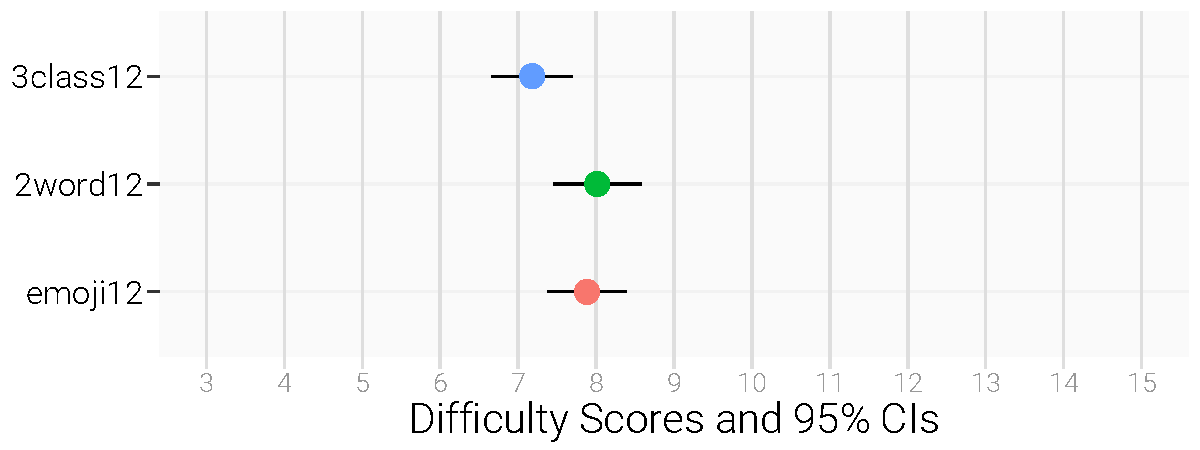
\includegraphics[width=\textwidth]{personality/difficulty-ci}
		\caption{\label{fig:personality:study-1-difficulty-ci}}
	\end{subfigure}
	\begin{subfigure}[t]{0.49\linewidth}
		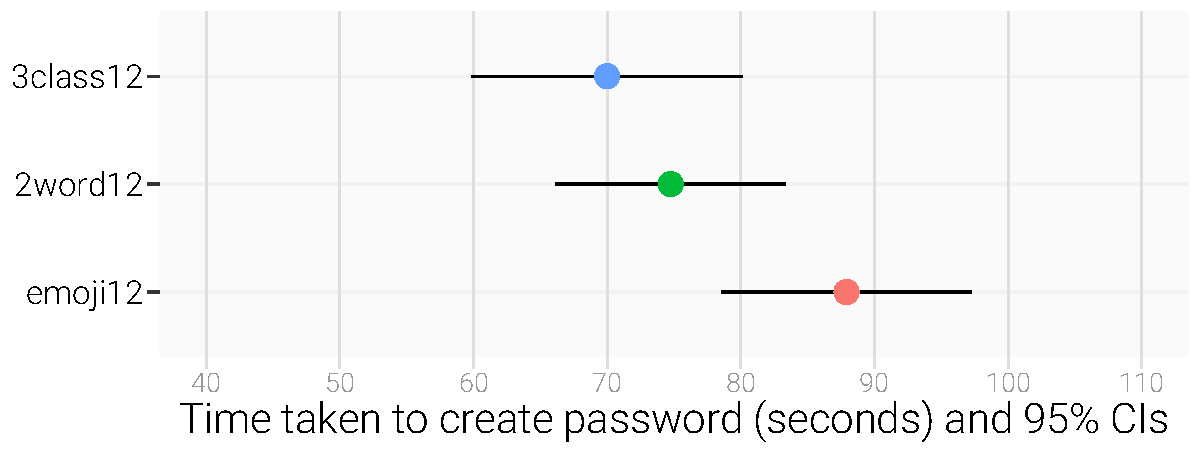
\includegraphics[width=\textwidth]{personality/timing-ci}
		\caption{\label{fig:personality:study-1-timing-ci}}
	\end{subfigure}
	\caption{\label{fig:personality:study-1-usability-stats}Confidence Intervals for a) Difficulty to create and b) time to create passwords in each condition. The traditional policy (3class12) was the easiest and fastest overall, but not on a statistically significant level (also visible in the charts due to the overlapping confidence intervals)}
\end{figure}
\subsubsection{Descriptives and Independent Variables}
Users rated the difficulty to create a password very similarly in all conditions (averages of scores in range [3;15]: 3class12 = 7.18, 2word12 = 8.02, emoji12 = 7.88). A linear mixed model ANOVA did not show significant differences (\statsgt{2+2}{5.28}{0.1}). Figure \ref{fig:personality:study-1-usability-stats} shows the confidence intervals for these two usability metrics ``difficulty to create'' and ``time to create''. Observing no significant differences overall is interesting because it means that individual ratings could be explained by personality traits. %TODO that's not quite clear.



%serial positioning effects do make a difference, but it also appears trivial in the overall sample.
%summary: no big difference between policies and ranking. (this is what makes the remainder more exciting, because a %closer look at the data brings out how the numbers come to be)

%%%%%%%%%%%
%%%%%%%%%%% Difficulty to create a password with a given policy
%%%%%%%%%%%
\subsubsection{Creation Difficulty Models}
The general additive models showed associations between the predictors and creation difficulty scores (see Table \ref{tab:personality:study-1-coffections-clean}). 
\begin{table}[htbp]
  \centering
    \begin{tabular}{l|SS|SS|SS}
          & \multicolumn{2}{c|}{\textit{emoji12}} & \multicolumn{2}{c|}{\textit{2word12}} & \multicolumn{2}{c}{\textit{3class12}} \\ \hline \hline
          (Intercept) & \multicolumn{2}{c|}{$9.99$} & \multicolumn{2}{c|}{$7.04$} & \multicolumn{2}{c}{$6.26$} \\ \hline
\multicolumn{1}{c|}{Predictor}  & \multicolumn{1}{c}{$\beta$} & \multicolumn{1}{c|}{$\sigma_n$} & \multicolumn{1}{c}{$\beta$} & \multicolumn{1}{c|}{$\sigma_n$} & \multicolumn{1}{c}{$\beta$} & \multicolumn{1}{c}{$\sigma_n$}  \\
    Age & 0.02  & 0.06  &       &       & -0.05 & 0.06 \\
    Gender (female) & 0.91  & 0.58  & 1.35  & 0.66  & -0.46 & 0.61 \\
    No IT Background & -0.10 & 0.59  & 0.60  & 0.66  & 0.21  & 0.63 \\
    Extraversion & -0.05 & 0.08  &       &       & -0.01 & 0.08 \\
    Conscientiounsness & 0.01  & 0.09  &       &       & 0.08  & 0.10 \\
    Neuroticism & -0.22 & 0.09  &       &       & 0.05  & 0.09 \\
    \textit{emoji12} Position 2 & 0.52  & 0.65  &       &       &       &  \\
    \textit{emoji12} Position 3 & 0.23  & 0.63  &       &       &       &  \\
    \textit{2word12} Position 2 &       &       & -0.38 & 0.74  &       &  \\
    \textit{2word12} Position 3 &       &       & -0.07 & 0.73  &       &  \\
    \textit{3class12} Position 2 &       &       &       &       & 1.19  & 0.66 \\
    \textit{3class12} Position 3 &       &       &       &       & 0.77  & 0.69 \\ \hline
%    edf: s(Age) & \multicolumn{2}{c|}{} & \multicolumn{2}{c|}{1.81} & \multicolumn{2}{c}{} \\
%    edf: s(Agreeableness) & \multicolumn{2}{c|}{3.27} & \multicolumn{2}{c|}{2.77} & \multicolumn{2}{c}{2.02} \\
%    edf: s(Openess) & \multicolumn{2}{c|}{2.50} & \multicolumn{2}{c|}{1.79} & \multicolumn{2}{c}{1.53} \\
%    edf: s(Extraversion) & \multicolumn{2}{c|}{} & \multicolumn{2}{c|}{1.52} & \multicolumn{2}{c}{} \\
%    edf: s(Conscientiousness) & \multicolumn{2}{c|}{} & \multicolumn{2}{c|}{3.32} & \multicolumn{2}{c}{} \\
%    edf: s(Neuroticism) & \multicolumn{2}{c|}{} & \multicolumn{2}{c|}{1.53} & \multicolumn{2}{c}{} \\ \hline
    Explained Deviance & \multicolumn{2}{c|}{0.15} & \multicolumn{2}{c|}{0.21} & \multicolumn{2}{c}{0.10} \\
    Num. Observations. & \multicolumn{2}{c|}{119} & \multicolumn{2}{c|}{119} & \multicolumn{2}{c}{119} \\
    Num. Smooth terms & \multicolumn{2}{c|}{2} & \multicolumn{2}{c|}{6} & \multicolumn{2}{c}{2} \\\hline
    \multicolumn{7}{l}{\textit{Description:}} \\ 
    \multicolumn{7}{l}{$\beta$ = Correlation coefficient} \\
    \multicolumn{7}{l}{$\sigma_n$ = standard error} \\
    \multicolumn{7}{l}{edf = estimated degrees of freedom by non-linear effects} \\
    \multicolumn{7}{l}{(\glqq estimated degrees of freedom\grqq)} \\
    \multicolumn{7}{l}{Smooth terms = non-linear effects in the model} \\
    \end{tabular}%
  \caption{Additive regression models for the difficulty to create passwords under the three policies.}
\label{tab:personality:study-1-coffections-clean}
\end{table}%
\paragraph{Control Variables} 
The GAM allowed us to model associations linearly for the control variables (example for emoj12 in Figure \ref{fig:personality:dc-emoji-b5}). Although we have to be careful not to generalize too strongly with our sample, linear associations at least enable us to use correlation coefficients $B$ as basis for discussion.
% gender
Female participants assessed it slightly more difficult to create passwords under the emoji12 ($B=0.91$) and 2word12 ($B=1.35, p<0.05$) policies than male participants. For 3class12, the correlation was smaller ($B=-0.46$) and pointed in the opposite direction. 
% it background
Having a background in IT positively showed medium correlations with difficulty in the 2word12 policy, too ($B=0.61$). This policy, albeit alphanumeric, is uncommon in the wild and ignores the verdict of high complexity -- IT people might be skeptical about the ``words'' requirement, while others are less concerned about it.
% order of the policy
The task order also showed medium-strong influence on creation difficulty. If emoji12 or 3class12 were part of the second task, creation was seen as more difficult ($B_{emoij12-pos2}=0.52$),  ($B_{3class12-pos2}=1.19$). 
% age
% we observed non-linear associations between age and creation difficulty, but the small age range forbids us to make conclusive inferences from our data.

%, too: emoji12 ($B=-0.10$) trivial, 3class12 ($B=0.21$) weak, 2word12  medium. it looks as though people with higher IT knowledge struggle with a word-based policy, potentially because it is much less common in the wild. 

\begin{figure}
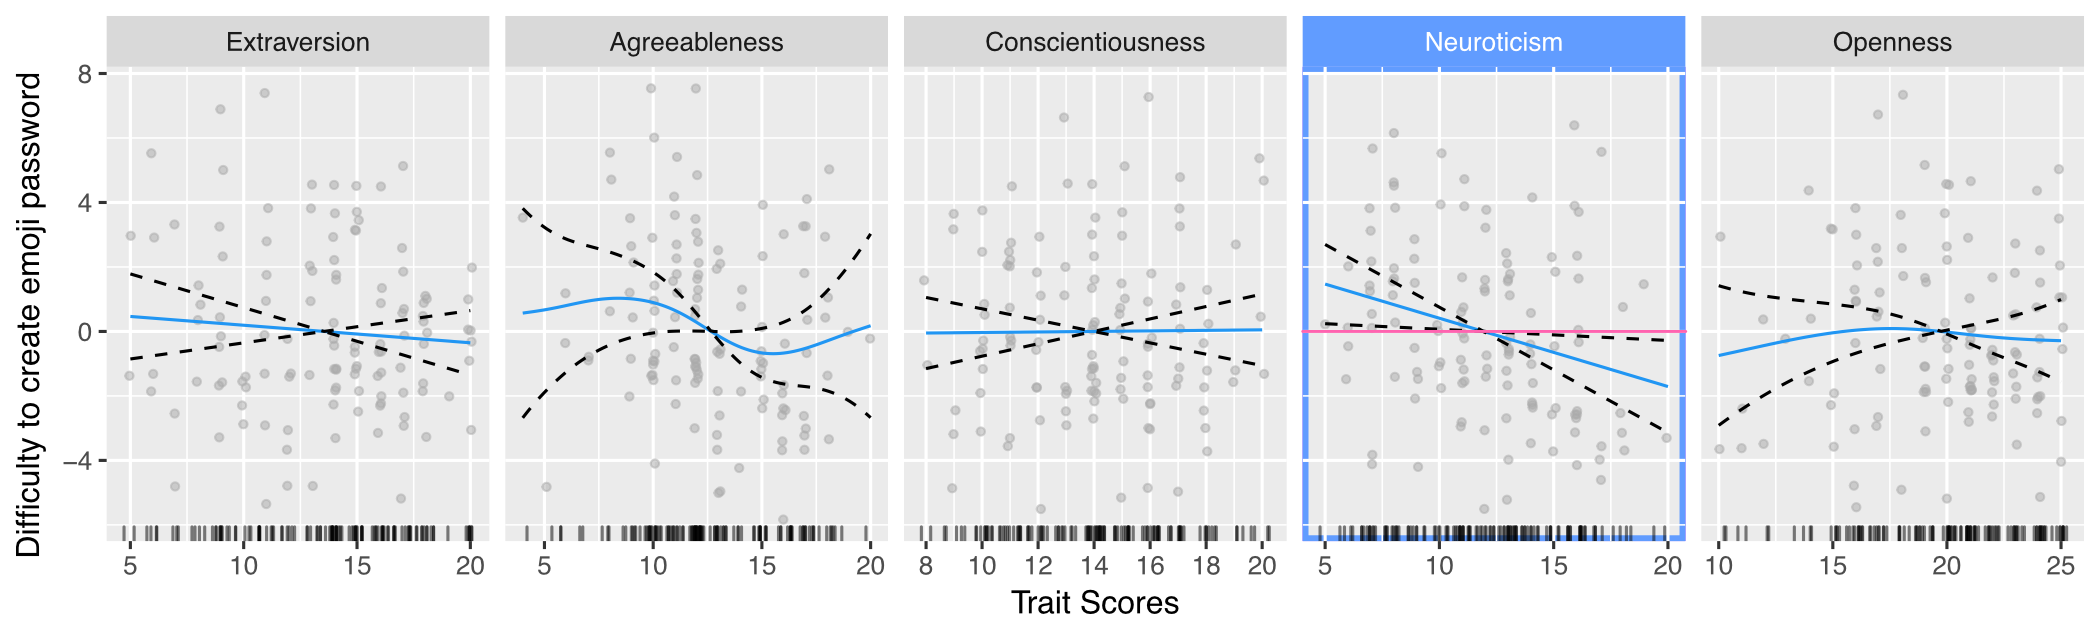
\includegraphics[width=\linewidth]{personality/png/dc-emoji-b5-v2}
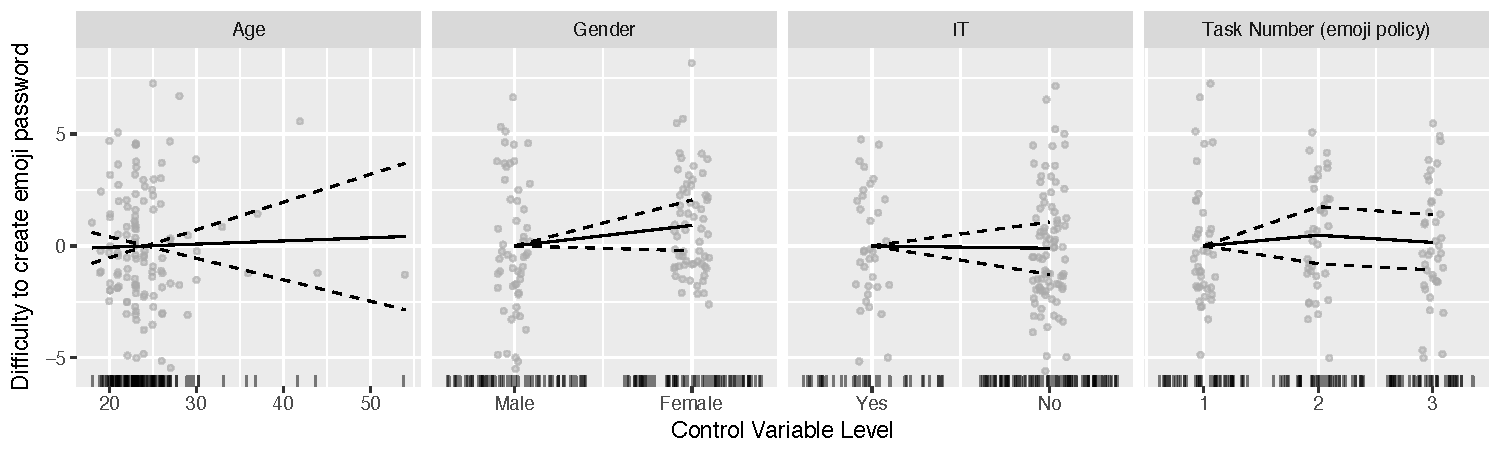
\includegraphics[width=\linewidth]{personality/png/dc-emoji-control-mod-v2}
\caption{\label{fig:personality:dc-emoji-b5}Associations between predictors and \textbf{difficulty} to create a password under the emoji12 policy. Charts visualize the functions derived from the Generalized Additive Models (GAMs). Neuroticism was significantly negatively associated with difficulty (highlighted in blue), i.e. it was easier to create emoji-passwords if participants scored high on neuroticism.}
\end{figure}

\noindent
\fbox{
	\label{sec:personality:study1:how-to-read-diagrams}
	\hspace{0.5cm}
	\centering
	\parbox[t][11.5cm]{0.9\linewidth}{
		\section*{How to Read Smoothed Regression Plots}\label{sec:personality:how-to-read-gam}
		\small
		Figure \ref{fig:personality:dc-emoji-b5} shows the first example of regression plots that will be used throughout the thesis where appropriate. There is a separate plot for each marginal association with a given predictor. The solid curve/line represents the estimated regression curve. If it is a straight line, the association can be modeled linearly (e.g. neuroticism in Figure \ref{fig:personality:dc-emoji-b5}). If it is a ``wiggly'' curve, the association is modeled with polynomial terms of different degrees (e.g. Agreeableness in Figure \ref{fig:personality:dc-emoji-b5}). The model intercept is at $y=0$. In many cases, residuals are plotted at their respective $(x,y)$ position to give a sense of clusters. At the bottom border of the plots, we often add ``rugs'' to show the number of observations/residuals along the x-axis. 
		
		Interpreting the effect size and significant contribution to the model fit is visible in two ways. First, the slope of the fitted line shows estimated strength of associations. Second, there are two dashed curves surrounding the fitted curve/line that visualize 95\% confidence intervals. Both curves are entirely above, respectively entirely below, the intersection between the fitted curve and the intercept at $y=0$, the association is significant at the 0.05 alpha level.
		
		In Figure \ref{fig:personality:dc-emoji-b5}, we highlighted this for the neuroticism plot. Left to the point of intersection, both dashed lines are above the intercept (in pink color); analogously, the dashed lines are below the intercept  on the right-hand side, indicating a significant contribution to the model. 
		
%		\begin{itemize}[leftmargin=*]
%			\item Personality is weakly associated with all the measured dimensions: strength perception, policy preference / usability, and password selection. Most notably openness and neuroticism showed conclusive associationes.
%			\item The models for the perception of passphrases achieved the highest fit, suggesting a predictable association between personality and strength perception for this type of password. Comparing two passwords was associated with the conscientiousness traits. Mixed models that use both password features and personality trait scores as covariates are the most feasible approach.
%			\item Older users might be the best target group for password support tools, because age was a good predictor of their usage. Suggesting good tools during account creation might lead to higher adoption 
%			%			\item Segmentation of users
%			\item Nudges designed for neuroticism should make emotional state more salient and highlight the benefits of \underline{long} passwords. 
%		\end{itemize}
	}
	\hspace{0.5cm}
}

\paragraph{Personality Traits}
Contrarily to the modeling functions for control variables, we mostly observed non-linear associations between trait scores and creation difficulty (see Figure \ref{fig:personality:dc-emoji-b5}).
%emoji personality
One exception is the weak linear association in the emoji12 ($B=-0.22$) condition. It tells us that it was slightly easier to create emoji-passwords for people with higher neuroticism scores. The neuroticism trait is also referred to as ``emotional stability'' \cite{Costa1992NEO}, i.e. neurotic people are usually more emotional. Expressing \textit{emotions} with emojis in passwords seems to support this trait and come easier to users scoring high on neuroticism. %(this is a great result, albeit weak. neurotic people are by defintion more \textit{emotional}, and emojis seem to cater to this trait.)

%agreeableness weak non linear, and interesting curve (up and down) for emoji12
%openness weak non linear, but too little data to conclusively decide. 

% 2word12 personality
%effects not as clear as for the emoji policy. highly open people report slightly less difficulty to create a 2word12 password.
In the models for the 2word12 policy, all associations were non-linear and thus inconclusive at this point. For the 3class12 policy, associations were linear but trivial for the extraversion, conscientiousness, and neuroticism factors. In summary, scores of the ``Creation Difficulty'' scale are difficult to explain with personality traits, but control variables appear to have stronger influence. Only neuroticism is associated notably with difficulty to create an emoji-password.
% 3class12
%linear associations are negligible for extraversion, conscientiousness, and neuroticism. 
%non-linear associations for agreeableness and openness. at value around 15 (from 20) the difficulty seems to increase (hard to interpret this finding). People with agreeableness scores of 18 and greater find it more difficult to create a 3class12 password by up to 1.5 points. Openness is inversely correlated here. the more open the participant was, the more likely they found it easy to create a 3class12 password. 

%%%%%%%%%%%
%%%%%%%%%%% Preference for one policy or another
%%%%%%%%%%%
\subsubsection{Policy Preference}
Table \ref{tab:pws_pers:distribution-binary-ranks} shows the overall preference for the three policies. It is evident that participants generally preferred the 3class12 policy (68\%). The emoji policy was best ranked by 18 participants, and 2word12 by 12 participants. Using logistic additive regression, we can determine the factors that contribute to these preferences. %https://web.stanford.edu/~hastie/Papers/AdditiveLogisticRegression/alr.pdf
In essence, the model gives us the likelihood of voting a given policy to the top, which is a binary decision (1 = preferred, 0 = not preferred). 
%did policy X land on top spot ? yes = 1, no = 1. thus, no encompasses the two other options.
%Logit model. 
\begin{table}
	\centering
	\caption{\label{tab:pws_pers:distribution-binary-ranks} Distribution of binary rankings of the three available policies. Evidently, 3class12 was ranked best in most cases. }
	\begin{tabular}{llll}
		~ 			& emoji12	& 2word12 	& 3class12 \\ \hline\hline
		1st rank	& 18		& 12		& 67 \\
		other rank 	& 80 		& 85 		& 31 \\ \hline
		n			& 98		& 98		& 98		 
	\end{tabular}
\end{table}

% predictors: demography and structure
Including demographic control variables as predictors, we observed strong effects for IT-background. The probability of putting emoji12 at the top is $exp(B{emoji-IT}) = 9.87$ for participants without technical background, so around ten times higher. Only one respondent with an IT background ranked emoji12 on the top. %This fits the finding that non-IT people found it easier to create an emoji12 password.
% order of policies 
The order in which policies were displayed also produced a notable effect. If emoji12 was part of the second $exp(B_{emoji-pos2}) = 0.27$ or third task $exp(B_{emoij-pos3}) = 0.76$, the likelihood to rate it the best policy slightly decreases. Other task orders, as well as age-related preferences, were inconclusive.

% personality
As with creation difficulty, rank-associations with personality traits were generally weak. The likelihood to prefer 2word12 decreased with higher extraversion scores $exp(B_{2word12-E}) = 0.82$. High agreeableness scores entailed higher chances to vote for emoji12 $exp(B_{emoji12-A}) = 1.28$. Interestingly, only very high neuroticism scores (>17) caused a  stark increase in favoring the emoji policy. However, the sample is thin in this area so the model is more unstable at this boundary. Other associations were negligible or inconclusive. 
%for agreeableness both linear and non-linear effects are visible; openness or conscientiousness have negligible, random associations. for neuroticism we lack data in edge cases (low or high trait scores) to draw conclusions. %there are more results in the BA, but I do not really see the point of reporting all the details of inconclusive results

%%%%%%%%%%%
%%%%%%%%%%% Password selection -- mostly emoji histogram
%%%%%%%%%%%
%\subsubsection{Password selection}

%\todo{create a emoiji selection histogram}. In essence, some emoji were strongly preferred, e.g. the red heart and the ``pouting face''. analyze: what were the usability ratings/rankings of those who picked the heart vs. the pouting face, i.e. are emojis with a positive connotation used by people who are happy that they can select an emoji password? I guess there are significant effects here. 

%TODO look into timings -- did conscientious people take longer to generate passwords?

\subsubsection{Time to Create Passwords}
The second usability metric was the time the participants took to create passwords. It can also be interpreted as \textit{effort} put into the task. The most interesting associations were visible for the 3class12 policy, where all personality traits could be modeled as linear predictors (see Figure \ref{fig:personality:timing-3class-b5}), and all showed medium-strong correlations (details in the Appendix, Table \ref{tab:personality:study-1:timing-models}). One might have suspected that conscientious people would invest more time, because one of their common attributes is diligence. However, this was not the case: conscientiousness was negatively associated with creation time for all policies ($B_{emoij12-C}=-3.58,B_{2word12-C}=-3.4,B_{3class12-C}=-2.09$). Neuroticism was significantly negatively associated with creation time, while agreeableness was marginally positively associated in 3class12. Demographic control factors indicated that, on average, women spent more time creating passwords in all conditions ($W=1166$, \pvallt{0.01}). The biggest effects were visible for task number as predictor: our participants took significantly less time to select passwords for the second and third tasks (example shown in \ref{fig:personality:timing-2word-control}). Most likely, this is a learning effect or due to people modifying their previous passwords. 


\begin{figure}
	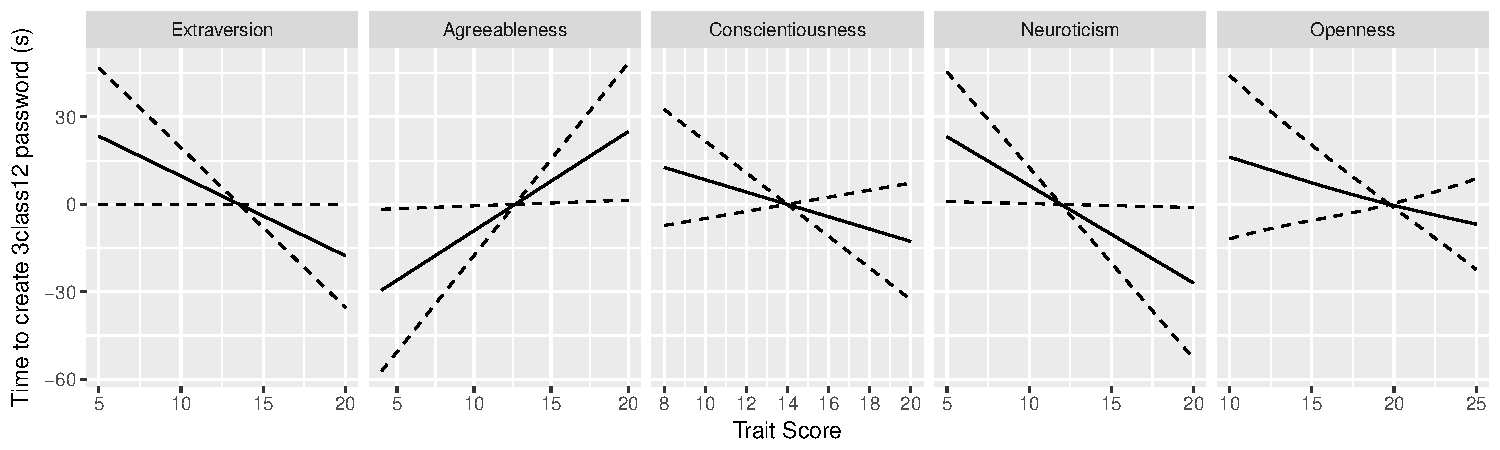
\includegraphics[width=\linewidth]{personality/timing-3class-b5}
	\caption{\label{fig:personality:timing-3class-b5}Associations between personality traits and time to create a 3class12 password. All traits could be modeled as linear predictors.}
\end{figure}

\begin{figure}
	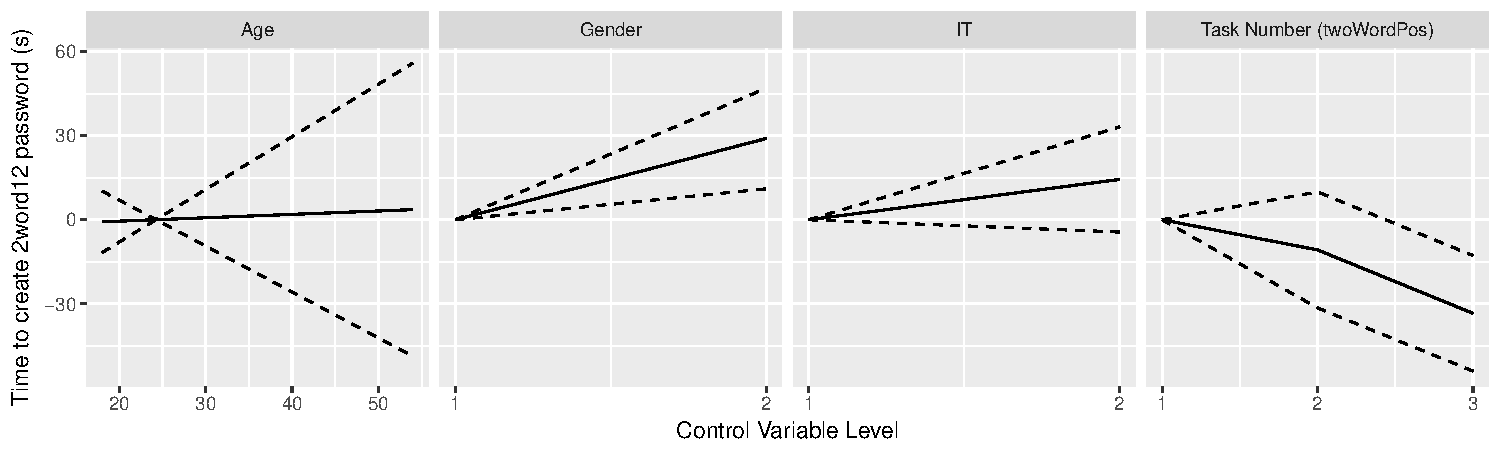
\includegraphics[width=\linewidth]{personality/timing-2word-control}
	\caption{\label{fig:personality:timing-2word-control}Associations between control variables and time to create a 2word12 password. Especially the task number and gender were showed strong associations.}
\end{figure}


%TODO the qualitative and plain-text passwords data is also interesting but goes too far at this point. 

\subsection{Finding Summary}
Overall, the usability metrics were comparable for all policies and the ranking was fairly homogeneous. So, any deviance from the mean could potentially be explained by personality traits and other confounding factors. In terms of personality, the most important finding was that scores on the neuroticism dimension seem to be positively associated with the usability of the emoji policy. As indicated above, emojis in passwords appear to fulfill their purpose in that they help some people express their emotions. Participants who did not have a background in IT were much more likely to prefer the emoji policy, and their neuroticism score played a subordinate role. Perhaps, a lack of expertise does not allow those participants to consider the switch from keyboard to mouse and vice versa (\textit{homing}). Moreover, the 3class12 policy received the most votes which might be due to the \textit{status quo bias} or \textit{familiarity bias}. 3class12 is the only commonplace policy among the tested ones, so participants were already used to it and voted it first. The timings were mostly affected by the task order -- participants spent less time on the second and third creation task. So although personality traits serve as predictors for timings, these effects were weaker by comparison. 

In summary, control factors had a greater effect on password usability and approval of policies than personality traits. Nonetheless, medium to strong effects are more likely to be detected with our sample size to begin with. So, the fact that we even observed small associations indicates that personality is a contributing factor to the perception of password policies. At this stage of the research we were not able to look into the selection behavior because the repeated measures design stood in the way. Thus, we designed and conducted two further studies to investigate the effect of personality on password strength perception and selection. 

%It could have been useful to include a recall test à la ``which passwords do you still remember after filling out the personality questionnaire?'' 

%medium associations between extraversion, agreeableness, and neuroticism (basically the other three dimensions that were not useful before), but control variables are associated to a larger degree.
%emoji policy similar results as traditional policies, i.e. it is wortwhile to experiment with it

%TODO re-read the discussion section, because the findings are a bit higher level and more understandable


%non linear associations probably explicable by other variables, e.g. intercorrelation -- 
%todo{discuss the personality traits and associations, try to explain them.}

%demographics play a role - (careful now, cowboy): policies could be tailored to gender. but i'm kind of reluctant to put this argument forward. at least IT background could be considered a factor for the policy. a personalized policy would make it more difficult for horizontal attacks because the policy is unpredictable.

%mutually exclusive effects for ranking are clear because of the binary nature.

%wild idea: if positioning influences the favorability of policies, one could leverage this. like anchoring and decoy (chose your own policy of the three). commitment and consistency as well (commit to your policy, create a strong password to be consistent with your commitment.)

%%%%%%%%%%%%%%%%%%%%%%%%%%%%%%%%%%%%%%%%%%%
%%%%
%%%%
%%%%			STUDY  2 TWO ZWEI
%%%%			PERCEPTION
%%%%
%%%%
%%%%%%%%%%%%%%%%%%%%%%%%%%%%%%%%%%%%%%%%%%%
\section{Study 2: Strength Perceptions}
With an observational online study, we explored the associations between psychological variables and password strength perception. We regard the perception of strength as necessary step before looking at actual behavior, which is more difficult to observe. Hence, we tried to find associations between subjective password strength ratings and scores on well-established psychometric scales. Before we ran the study, we pre-registered the experiment with the open-science framework (OSF)\footnote{\url{https://osf.io/}, last accessed 11.09.2016} and conducted all analyses as predicted to mitigate confirmation bias. Since we consider our research efforts mostly exploratory, we approached the study without specific hypotheses regarding the influence of certain personality traits or decision making styles on the perception of password strength.

\subsection{Structure}
% DEMOGRAPHICS
The study was divided into six parts of which two were standard psychometric tests. After a brief introduction where the participants were informed about the background of the study, they answered basic demographic questions about gender, age, educational and professional background. %This information is important for the ratings on the password scales, because advanced knowledge in IT(-security) may lead to a different rating than the general audience. 

% META STATISTICS / CREATION
The second part was about collecting characteristics about the passwords that our participants used on real online accounts. Here, we asked about typical password attributes, like LUDS (lower-, uppercase, digits, symbols), length and the inclusion of dictionary words. The collection of such password descriptions is an ethically reasonable way to study actual behavior that does not directly involve creating and disclosing an entire password \cite{VonZezschwitz2013SurvivalShortest}. Participants could select from a list of accounts that they used on a regular basis, e.g. Facebook, YouTube, Netflix, Google. If they did not have any of the selectable accounts they could provide another. The description of a participant's password is called \textit{meta password} in the remainder of the paper. 
%TODO entscheiden ob das reinkommt Additionally we had them create a password which they would rate as sufficient to protect such an online account and that is memorable. We asked not to enter a password that they were currently using. At the end of the study, we again inquired after the fictional password to measure short-term memorability. 


%%% TABLE: PASSWORDS
\begin{table}[htbp]
  \centering
  \caption{Set of passwords that we divided into different length and strength categories (as measured with zxcvbn). Features: U = uppercase, D = digits, S = symbols}
 % \small
    \begin{tabular}{lllcccr}
    \multicolumn{1}{c}{\multirow{2}[1]{*}{Password}} & \multicolumn{2}{c}{Categories} & \multicolumn{3}{c}{\multirow{2}[1]{*}{Features}} & \multicolumn{1}{c}{guesses} \\
      & Length & Strength & \multicolumn{3}{c}{} & \multicolumn{1}{c}{(log10)} \\
    \midrule
    hagrqqqqthhbbe & Long & Strong & \multicolumn{3}{c}{-} & 12.48 \\
    etuhcarap & Short & Weak & \multicolumn{3}{c}{-} & 4 \\
    AbWxCdYz & Short & Medium & \multicolumn{3}{c}{U} & 8 \\
    1qaz2wsx3edc & Long & Weak & \multicolumn{3}{c}{D} & 3 \\
    a6a4ba8a & Short & Medium & \multicolumn{3}{c}{D} & 8 \\
    ieatkale88 & Short & Medium & \multicolumn{3}{c}{D} & 10 \\
    thedzfhg123 & Short & Medium & \multicolumn{3}{c}{D} & 10 \\
    11Nd1sPPut8ble99 & Long & Strong & \multicolumn{3}{c}{U,D} & 16 \\
    bicycles-peaches-cold & Long & Strong & \multicolumn{3}{c}{S} & 13.69 \\
    AatIcs,ijayl-t & Long & Strong & \multicolumn{3}{c}{U,S} & 13.95 \\
    p@ssw0rd & Short & Weak & \multicolumn{3}{c}{D,S} & 0.95 \\
    ocean4 Size !beer Car & Long & Strong & \multicolumn{3}{c}{U,D,S} & 20.39 \\
    F@m1Ly07\% & Short & Medium & \multicolumn{3}{c}{U,D,S} & 6.88 \\
    \bottomrule
    \end{tabular}%

  \label{tab:password-list}%
  
\end{table}%

%  RATING
In the third part of the study, the \textit{rating part}, the participants assessed the strength of one password at a time in random order. The passwords had to be rated on 7-point scales ranging from \textit{1 = very weak} to \textit{7 = very strong}. We picked a set that was comparable to related work \cite{Ur2016PerceptionsPassword} and that we carefully designed around certain attributes. Table \ref{tab:password-list} shows the selected set of passwords and their features. The ``length'' category distinguishes between short passwords with nine characters or less and long passwords with ten characters or more. The distinction is inspired by real-world policies that usually require nine or more characters \cite{Wang2015EmperorsPolicies}. Other passwords are usually ``below that bar'' and can thus be considered too short. The ``strength'' category groups passwords on three levels by their objective guessability as measured by zxcvbn. Weak passwords require less than $10^{6}$ guessing attempts, strong passwords at least $10^{12}$ guesses, and medium passwords anything in between. This classification is in concordance with related work \cite{Florencio2014AdministratorsGuide, Wheeler2016zxcvbn} . To fully counterbalance all category combinations, one would require 120 items, which we could not implement for the sake of brevity. Hence, we kept the number of items small to mitigate fatigue during the study sessions. In the chosen set of 13 passwords, there were at least three items for each distinct category, i.e. three short, long, weak and strong passwords, and at least three passwords containing at least one of LUDS features (lowercase, uppercase, digits and symbols)

% COMPARISON
Following a similar procedure as Ur et al. \cite{Ur2016PerceptionsPassword}, participants moved on to compare the strength of passwords pairs (\textit{comparsion part}). The 7-point scale ranged from ``<left password> is much stronger'' to ``<right password> is much stronger''. The pairs were constructed such that the passwords differed, e.g., in the existence and positions of digits and uppercase letters. Figure \ref{fig:comparisontask} illustrates our scoring schema. 

\begin{figure}
	\centering
	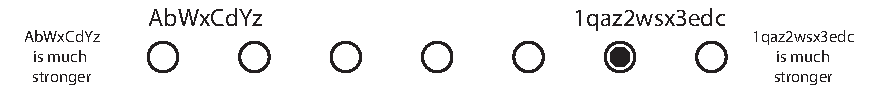
\includegraphics[width=\linewidth]{figures/comparisontask}
	\caption{\label{fig:comparisontask} Simplified item of the comparison task. The passwords differ in length, strength, and the usage of uppercase letters and digits. Here would have scored the importance of length and digits with +2 while the importance of strength and uppercase letters was scored with -2.}
\end{figure}

If the passwords measurably differ in strength as in Figure \ref{fig:comparisontask}, the ratings show if the participants' perceptions match reality. In total, ten comparisons had to be made in random order, in which we permuted the combinations. For this task, we also added an attention check where the passwords on both sides of the scale matched, allowing us to exclude responses where the answer differed from ``both passwords are equally strong''. 

Next, we requested self-assessment about security-related behavior using the Security Behavior Intentions Scale (SeBIS) \cite{Egelman2015SeBIS}. This scale comprises the dimensions \textit{securement}, \textit{passwords}, \textit{awareness}, and \textit{updating}. For each dimension, a score is calculated with four items totaling up to 16 additional items in our study. However, in discussions after the experiment we received hints that it would have been better to include a gap of a couple of days before collecting the SeBIS data to ensure its validity. Since we failed to take this into account beforehand, we do not report the results further, but it is important to mention that the questionnaire included 16 additional items. 
%The items are phrased as statements to which respondents can indicate how often they show a certain type of security-related behavior. The scale ranges from \textit{1 = never} to \textit{5 = always}. The \textit{password} dimension measures general attitude towards passwords, which we can utilize to inform our interpretation later.

The study concluded with two psychometric tests. In the \textit{Big-Five part}, we utilized a set of 50-items from the International Personality Item Pool (IPIP), which is a representation of Costa and McCrae's NEO-PI-R domains \citep{Costa1992NEO}\footnote{All items of the personality test can be found here: \url{http://ipip.ori.org/newNEODomainsKey.htm}, psychometric properties: \url{http://ipip.ori.org/newNEO_DomainsTable.htm}}. In this personality test, participants rate how accurately a certain statement portraying a certain personality characteristic describes themselves. Each item is a 5-point scale with the labels \textit{very inaccurate, moderately inaccurate, neither accurate nor inaccurate, moderately accurate, very accurate}. Every personality trait is tested with five positively and five negatively keyed items. It was shown that the 50-item version of the test shows high correlation with more exhaustive tests ($r > 0.75$ in all dimensions) and is thus a sufficiently reliable test. We randomized the order of the items.

Egelman and Peer found that the general decision making style had higher predictive power than the Big-Five traits for privacy-related behavior \cite{Egelman2015AverageUser}. Thus, we wanted to test the feasibility of both psychometric tests and finished the study with the \textit{GDMS part}. This scale uses 25 positively keyed items to measure the five decision-making styles \textit{rational}, \textit{intuitive}, \textit{dependent}, \textit{avoidant} and \textit{spontaneous}. 

\subsection{Quantitative Analysis}
We used a set of statistical tests to explore the relationship between the scores psychometric scales and password strength perception. Since at least three passwords showed a certain characteristic, e.g. uppercase letters, we averaged the ratings for them accordingly. Moreover, in the psychometric tests we accounted for negatively keyed items, i.e. those items that were phrased with negations like \textit{``I don't talk a lot''}. We inverted the ratings where necessary and afterwards calculated the sum of agreement for each dimension. 

We use linear regression with subjective password strength assessments as dependent variables. We calculate one score per participant and password category by averaging the corresponding ratings. Psychometric test results on sub-scales served as independent variables. We always control the regression models for gender, technical background and education level to prevent misinterpreting the effects. Education was coded as ordinal variable from 1 (grammar school) to 7 (professional degree like PhD, MD, JD). We check for collinearity using variance inflation factors (VIF) and only retain factors with VIFs close to 1 \cite[p. 217]{Weisberg2005applied}. Also, because of the exploratory nature, we can use step-wise regression methods to build the models. To mitigate type-II errors herein, we use a backward approach \cite[p. 161]{Field2005DiscoveringStatistics} and exclude factors that do not improve the model significantly. Finally, we perform Durbin-Watson tests to rule auto-correlation effects (target value $d=2$). While p-values do not add much to the interpretability of the findings, we report them for the sake of completeness.  
%TODO Quelle!
%Our level for statistical significance is $\alpha = 0.05$, unless Bonferroni correction requires a lower value. 

When we report the results of linear regression models, we only do so for the models with the highest adjusted $R^2$ value, i.e. the model where the number of predictors leads to the best model-fit explaining the variance in the dependent variable. The values in Tables \ref{tbl:personalpw_regression} through \ref{tab:Comparison-Regression} are the \textbf{standardized beta} correlations, i.e. they are unit-less and lie between -1 and +1. 

\subsection{Qualitative Analysis}
To better understand the reasoning behind the ratings and comparisons, we also inquired how the respondents approached the rating task. They could enter free-text answers after all ratings were done. The answers were then coded independently by two members of the team. The first coding step was to find categories and propose the code book. Afterwards, the proposed codes were handed over to the second coder, who sorted answers into the categories and amended new ones where necessary. Interrater agreement between the two coders was satisfactory (78\%, Krippendorff's $\alpha = 0.55$) and the final the code book could be created after discussing the discrepancies. We report how many participants mentioned a particular theme in their response regarding their rating strategies.


\subsection{Recruitment}
We utilized the online research platform Prolific\footnote{\url{https://prolific.ac}, accessed 01.09.2016} to administer our survey. Participants received \$2.65 upon successful completion, which took 20 minutes in average. This compensation level is suggested as part of the ethical reward guidelines on the platform. Only an English-speaking audience was eligible to participate. From the 178 people who started the survey, 104 finished it. To prevent low quality answers, we introduced an attention check during the comparison part of the experiment.  

%In the first phase of the study, the participants were asked to imagine their email provider required them to create a new password and they could not select their current one. This measurement was taken early to prevent bias from showing different types of passwords. The answers were collected in plain text. We proceeded to have the users choose the type of account that they would be willing to secure with their selected password in the real world. This would indicate the effort and the value of their selection.


\subsection{Ethical Considerations}
There is no institutional review board for this kind of studies at our institution. However, we designed the questionnaire to respect the participants' privacy and did our best to minimize the level of disclosure of sensitive data. The metrics we collected to characterize the participants' passwords are most likely insufficient to reconstruct the passwords in a straightforward way and can thus be considered ethically acceptable. 


\subsection{Limitations}
%It is good to discuss the limitations before the results. Thus, the reader can bear them in mind when they are reading on. 

Like most studies involving personality assessment, the result is only a rough model of a person's personality and does not include all facets. We chose a test with 50 items to assess the Big-Five traits. While such psychometric tests exist with item counts between 10 \cite{Gosling2003TIPI} and 240 items \cite{Costa1992NEO}, the 50-item version has high internal reliability and does not fatigue the respondents as much as more exhaustive tests. Additionally, with a sample size of 100 participants, power-analysis tells us, that only strong and medium interactions are likely to be found for with our regression models (cf. \cite{Shevlin1998SampleSize} or \cite[p. 223]{Field2005DiscoveringStatistics}). At this stage of the exploration, however, this is what we aimed for. If we do find effects with such a small sample, then they must be large enough to justify follow-up investigations with larger samples. 

Furthermore, the methodology relies on self-assessment and honest answers, which are difficult to control. We introduced an attention check to mitigate the problem, by asking people to compare two identical passwords. For the meta-password, we do not know whether it was created on a mobile or desktop device. Passwords created on mobiles are usually less complex than those created on desktops \cite{Melicher2016UsabilityMobileTextPasswords, VonZezschwitz2014HoneyIShrunkTheKeys}. 

We also have to be careful not to over-generalize the results due to our use of crowd-sourced study participation. The responses may not be representative for a larger population, e.g. because the sample stems from a technically savvy audience. Users registering for tools like Prolific or Amazon Mechanical Turk may also have stronger financial motivation to do so than the rest of the population \cite{Ross2010WhoAreTurkers}. 

Finally, the study set-up and procedure may also influence the interpretability of the outcome. We decided not to randomize the order of the question blocks to maintain full control over the general procedure. When we measure dependent variables, the order of questions is still randomized in the question groups. This way, the potential fatigue effects are the same for all participants at the different stages, while the important questions are in random order. Moreover, the items for password pairs were not fully counterbalanced on all levels to prevent fatigue when answering the entire questionnaire. A more exhaustive set of tested passwords would increase the generalizability. 

%we need to be aware that a more faceted personality profile may reveal larger differences. 
%TODO viele antworten deuteten darauf hin, dass englisch nicht in die muttersprache ist. 
%TODO meta password characteristics are not an accurate proxy for password strength, as depicted in the background section. 
%Our proxy for password strength is the result of the zxcvbn estimator algorithm \cite{Wheeler2016zxcvbn}. While it can estimate the strength of passwords in attack scenarios up to one million guesses, its estimates become more fuzzy above this threshold. However, for the purpose of the study, the estimate was considered good enough as it still highly correlates with the estimates of more sophisticated tools like the password guessing service (PGS) \cite{Ur2015MeasuringRealWorldAccuracies}. 
%\begin{itemize}
%\item we might measure intelligence
%\item self-reporting might not be accurate
%\end{itemize}


%As we collected plain text passwords that could -- in theory -- be linked backed to an individual, we took special care to point out that participants should not enter their actual password, but to think of a new one. The additional meta characteristics are most likely insufficient to reconstruct a participant's actual password. 

\begin{figure}
	\centering
	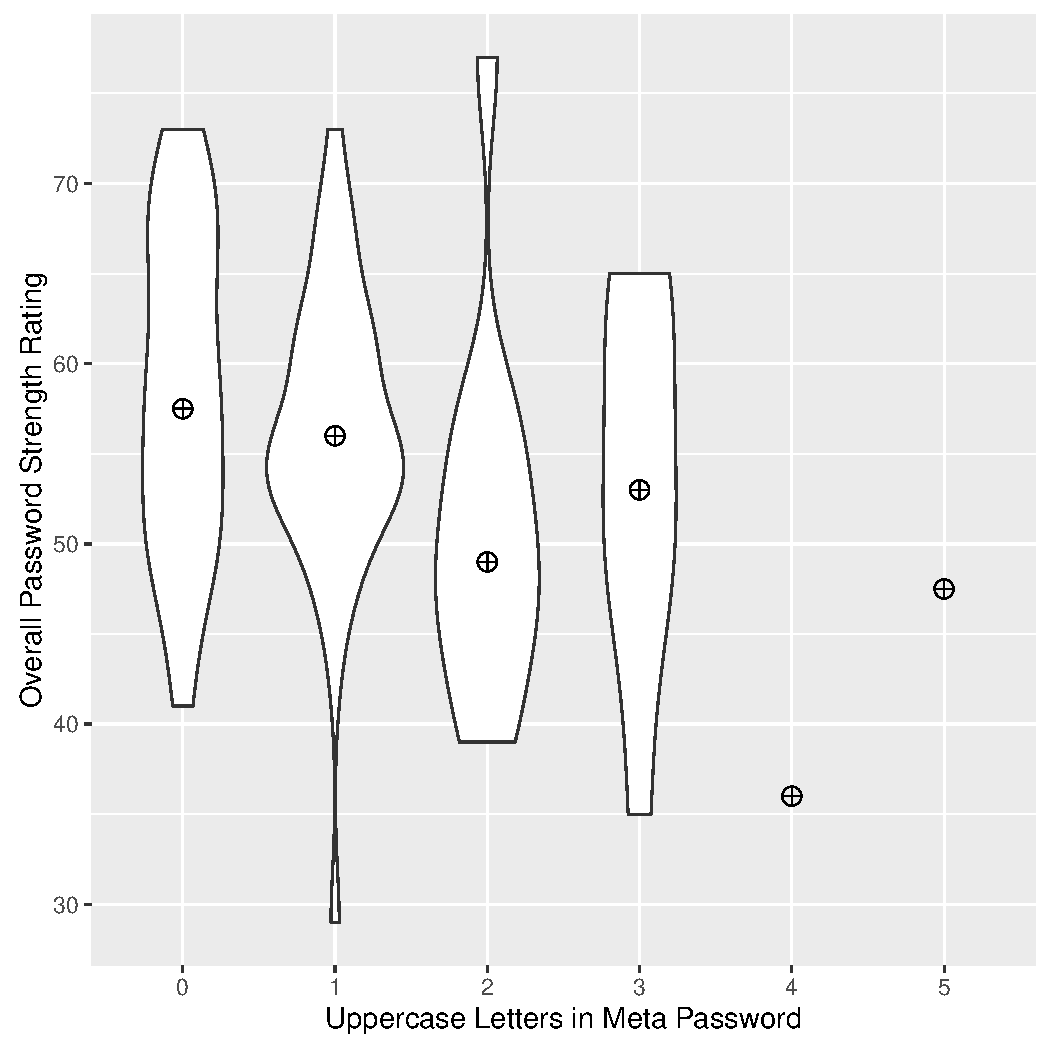
\includegraphics[width=\linewidth]{figures/MetaPW-Violinplot}
	\caption{\label{fig:MetaPW-ViolinPlot} Violin plot of strength ratings, grouped by the number of uppercase letters in the participants' meta password. The plot gets broader, the more respondents scored in the particular range. The plot shows a negative association between overall password strength and uppercase letters in the meta password.}
\end{figure}



%%%%%%%%%%%%%%%%%%%%%%%%%%%%%%%%%%%%%%%%%%%
%%%%
%%%%
%%%%			RESULTS 
%%%%
%%%%
%%%%%%%%%%%%%%%%%%%%%%%%%%%%%%%%%%%%%%%%%%%
\subsection{Results}
In this section, we first describe the participants and meta password characteristics before we proceed to the regression analyses. The final part of this section shows qualitative findings and a brief synthesis of the results. 

\subsubsection{Participants}
We collected 104 complete samples. We had to remove three samples from respondents who failed the attention check. Another response was removed because all responses on point scales were answered with the same value. This procedure is proposed by the IPIP project \footnote{\url{http://ipip.ori.org/newValidity.htm} accessed 02.09.2016}. The resulting total N = 100 was divided into 42 female and 58 male participants. Their average age was 28 years ($Standard Deviation~(SD) = 9,~Minimum = 16,~Maximum = 61,~Median~(Md) = 26$). 44 responses came from students. The education level was high with 59 participants reportedly having a bachelor's (44) or master's (15) degree. 29 participants claimed to have a computer science or IT-related background. In summary, our sample stems from a young, educated and fairly technically savvy population. This convenience sample is not ideal, but we hope to deal with this skew by including demographics as predictors in the regression models.

\subsubsection{Strength Categories and Meta Passwords}
On average, the respondents correctly identified weak, medium and strong passwords in the rating task, i.e. their perception matched reality. The average scores were $M=3.60~(SD=1.07)$ for weak, $M=4.25~(SD=0.95)$ for medium and $M=4.71~(SD=0.90)$ for strong passwords. A Friedman rank test showed that these ratings differed significantly ($F(2)=59.91,~p < 0.001$). 

%%%%%% TABLE 
\begin{table*}%[h!tbp]
  \small
  \centering
  \caption{Regression analysis for password ratings in different categories as dependent variables and psychometrics as independent variables variables. Demographic data serves as control variables. Numbers in bold indicate statistical significance ($p<0.05$). The Big-Five factors had higher predictive value and than the GMDS factors.}
    \resizebox{\linewidth}{!}
{
\begin{tabular}{rl|r|rr|rrr|rrr}
    \multicolumn{2}{l|}{Predictor} & \multicolumn{1}{l|}{Overall} & \multicolumn{1}{l}{Short} & \multicolumn{1}{l|}{Long} & \multicolumn{1}{l}{Weak} & \multicolumn{1}{l}{Medium} & \multicolumn{1}{l|}{Strong} & \multicolumn{1}{l}{Symbols} & \multicolumn{1}{l}{Digits} & \multicolumn{1}{l}{Uppercase} \\
\cmidrule{3-11}    \rowcolor[rgb]{ .718,  .871,  .91} \multicolumn{1}{l}{Big Five} & Neuroticism & \cellcolor[rgb]{ 1,  1,  1}  & \cellcolor[rgb]{ .949,  .91,  .518} 0.15 & \cellcolor[rgb]{ .949,  .91,  .518} 0.15 & \cellcolor[rgb]{ .969,  .914,  .518} 0.14 & \cellcolor[rgb]{ 1,  1,  1}  & \cellcolor[rgb]{ .98,  .627,  .459} -0.15 & \cellcolor[rgb]{ 1,  1,  1}  & \cellcolor[rgb]{ 1,  1,  1}  & \cellcolor[rgb]{ 1,  1,  1}  \\
    \rowcolor[rgb]{ .718,  .871,  .91}   & Openness & \cellcolor[rgb]{ .976,  .518,  .439} \textbf{-0.25} & \cellcolor[rgb]{ .976,  .541,  .443} \textbf{-0.23} & \cellcolor[rgb]{ .98,  .573,  .447} \textbf{-0.2} & \cellcolor[rgb]{ .976,  .498,  .435} \textbf{-0.27} & \cellcolor[rgb]{ .98,  .616,  .459} -0.16 & \cellcolor[rgb]{ .98,  .604,  .455} -0.17 & \cellcolor[rgb]{ .984,  .647,  .463} -0.13 & \cellcolor[rgb]{ .976,  .541,  .443} \textbf{-0.23} & \cellcolor[rgb]{ .984,  .639,  .463} -0.14 \\
    \rowcolor[rgb]{ .718,  .871,  .91}   & Agreeableness & \cellcolor[rgb]{ .898,  .894,  .514} 0.18 & \cellcolor[rgb]{ .949,  .91,  .518} 0.15 & \cellcolor[rgb]{ .898,  .894,  .514} 0.18 & \cellcolor[rgb]{ .898,  .894,  .514} 0.18 & \cellcolor[rgb]{ 1,  1,  1}  & \cellcolor[rgb]{ .969,  .914,  .518} 0.14 & \cellcolor[rgb]{ .984,  .918,  .518} 0.13 & \cellcolor[rgb]{ .996,  .91,  .514} 0.11 & \cellcolor[rgb]{ 1,  1,  1}  \\
    \rowcolor[rgb]{ .988,  .835,  .706} \multicolumn{1}{l}{GDMS} & Rational & \cellcolor[rgb]{ 1,  1,  1}  & \cellcolor[rgb]{ 1,  1,  1}  & \cellcolor[rgb]{ 1,  1,  1}  & \cellcolor[rgb]{ 1,  1,  1}  & \cellcolor[rgb]{ 1,  1,  1}  & \cellcolor[rgb]{ 1,  1,  1}  & \cellcolor[rgb]{ 1,  1,  1}  & \cellcolor[rgb]{ 1,  1,  1}  & \cellcolor[rgb]{ .984,  .918,  .518} 0.13 \\
    \rowcolor[rgb]{ .988,  .835,  .706}   & Intuitive & \cellcolor[rgb]{ 1,  1,  1}  & \cellcolor[rgb]{ 1,  1,  1}  & \cellcolor[rgb]{ 1,  1,  1}  & \cellcolor[rgb]{ 1,  1,  1}  & \cellcolor[rgb]{ 1,  1,  1}  & \cellcolor[rgb]{ 1,  1,  1}  & \cellcolor[rgb]{ 1,  1,  1}  & \cellcolor[rgb]{ 1,  1,  1}  & \cellcolor[rgb]{ .996,  .898,  .51} 0.1 \\
    \rowcolor[rgb]{ .988,  .835,  .706}   & Avoidant & \cellcolor[rgb]{ 1,  1,  1}  & \cellcolor[rgb]{ 1,  1,  1}  & \cellcolor[rgb]{ 1,  1,  1}  & \cellcolor[rgb]{ .984,  .639,  .463} -0.14 & \cellcolor[rgb]{ 1,  1,  1}  & \cellcolor[rgb]{ 1,  1,  1}  & \cellcolor[rgb]{ .984,  .647,  .463} -0.13 & \cellcolor[rgb]{ 1,  1,  1}  & \cellcolor[rgb]{ 1,  1,  1}  \\
    \rowcolor[rgb]{ .988,  .835,  .706}   & Spontaneous & \cellcolor[rgb]{ 1,  1,  1}  & \cellcolor[rgb]{ 1,  1,  1}  & \cellcolor[rgb]{ 1,  1,  1}  & \cellcolor[rgb]{ 1,  1,  1}  & \cellcolor[rgb]{ .984,  .918,  .518} 0.13 & \cellcolor[rgb]{ 1,  1,  1}  & \cellcolor[rgb]{ .949,  .91,  .518} 0.15 & \cellcolor[rgb]{ 1,  1,  1}  & \cellcolor[rgb]{ 1,  1,  1}  \\
      & Education &   & \cellcolor[rgb]{ .914,  .898,  .514} 0.17 &   & \cellcolor[rgb]{ .984,  .918,  .518} 0.13 & \cellcolor[rgb]{ 1,  .922,  .518} 0.12 &   &   & \cellcolor[rgb]{ .933,  .902,  .514} 0.16 &  \\
      & CS Background & \cellcolor[rgb]{ .984,  .647,  .463} -0.13 &   & \cellcolor[rgb]{ .984,  .647,  .463} -0.13 &   & \cellcolor[rgb]{ .98,  .627,  .459} -0.15 & \cellcolor[rgb]{ .984,  .682,  .471} -0.1 &   & \cellcolor[rgb]{ .984,  .682,  .471} -0.1 &  \\
    \midrule
      & F & 4.23 & 2.83 & 3.54 & 3.46 & 1.9 & 2.48 & 1.91 & 2.52 & 1.19 \\
      & df & 3 & 4 & 4 & 5 & 4 & 4 & 4 & 4 & 3 \\
      & p & < 0.01 & < 0.05 & < 0.05 & < 0.01 & > 0.1 & < 0.05 & > 0.1 & < 0.05 & > 0.1 \\
      & R$^2$ & \cellcolor[rgb]{ .761,  .898,  .804} 0.12 & \cellcolor[rgb]{ .788,  .91,  .827} 0.11 & \cellcolor[rgb]{ .733,  .886,  .78} 0.13 & \cellcolor[rgb]{ .675,  .863,  .729} 0.15 & \cellcolor[rgb]{ .906,  .957,  .929} 0.07 & \cellcolor[rgb]{ .82,  .922,  .855} 0.1 & \cellcolor[rgb]{ .906,  .957,  .929} 0.07 & \cellcolor[rgb]{ .82,  .922,  .855} 0.1 & \cellcolor[rgb]{ .988,  .988,  1} 0.04 \\
      & Adjusted R$^2$ & \cellcolor[rgb]{ .706,  .875,  .757} 0.09 & \cellcolor[rgb]{ .776,  .906,  .82} 0.07 & \cellcolor[rgb]{ .706,  .875,  .757} 0.09 & \cellcolor[rgb]{ .635,  .847,  .698} 0.11 & \cellcolor[rgb]{ .882,  .949,  .91} 0.04 & \cellcolor[rgb]{ .812,  .918,  .851} 0.06 & \cellcolor[rgb]{ .918,  .961,  .941} 0.03 & \cellcolor[rgb]{ .812,  .918,  .851} 0.06 & \cellcolor[rgb]{ .988,  .988,  1} 0.01 \\
    \bottomrule
    \bottomrule
    \end{tabular}%
}
  \label{tab:Regression-Rating}%
\end{table*}%

%%%%%%%%%%%%%%%%%%%%%%%%%%
%%% 
%%% 		STRENGTH RATING
%%% 
%%%%%%%%%%%%%%%%%%%%%%%%%%
\subsubsection{Standalone Strength Rating}
Our next step was to analyze associations between personality, respectively decision making style and password perception. After having done all required assumption checks, including internal consistency analysis of the scales ($\alpha_{IPIP}=0.72, \alpha_{GDMS}=0.8$), we built regression models containing the scores on the big-five subscales, the GMDS scores and control variables. The initial model hence included the independent variables \textit{openness, conscientiousness, extraversion, agreeableness, neuroticism}, as well as the \textit{rational, intuitive, dependent, avoidant, spontaneous} decision making scores. We added gender, IT-background and education level as controlling factors. The initial model contained all factors and was refined in a backward stepwise removal approach, leaving only those factors with highest predictive values. 

Table \ref{tab:Regression-Rating} shows the regression results of standalone password ratings. The overall ratings in the first column, which we consider the most important metric, were negatively associated with the \textit{openness} trait ($\beta = -0.25, p < 0.05$) (see also Figure \ref{fig:openness-scatterplot}). In other words, participants with higher openness scores were generally more pessimistic regarding password strength, which was also the case if participants had a technical background, albeit this association was not as strong. Higher agreeableness scores were slightly associated with more optimistic overall password ratings. Interestingly, with conscientiousness and extraversion, two of the big-five factors never played a significant role and thus are omitted in Table \ref{tab:Regression-Rating}.

The decision making style predictors were retained in four of the nine models, but never showed high predictive power. Contrarily, the openness trait was retained in the regression models across the board. For example, especially the weaker passwords receive lower ratings from people with higher openness scores. However, the average adjusted $R^2$ across all categories tells us that the models explain only a rather small portion of the variance in the password ratings ($M=0.06~(SD=0.03)$). 

%The lower half of Table \ref{tab:B5-Regression-Comparison} shows the analysis results for standalone password ratings. One can see that there were no striking associations between predictors and dependent variables. Also, the models with the highest $R^2$ value needed six degrees of freedom on average. This means that no particular decision making style stands out to inform the predictions. The maximum $R^2$ value across the models here is $0.05$, i.e. very low. Thus, decision making style did not explain variances satisfactorily.

\begin{figure}
	\centering
	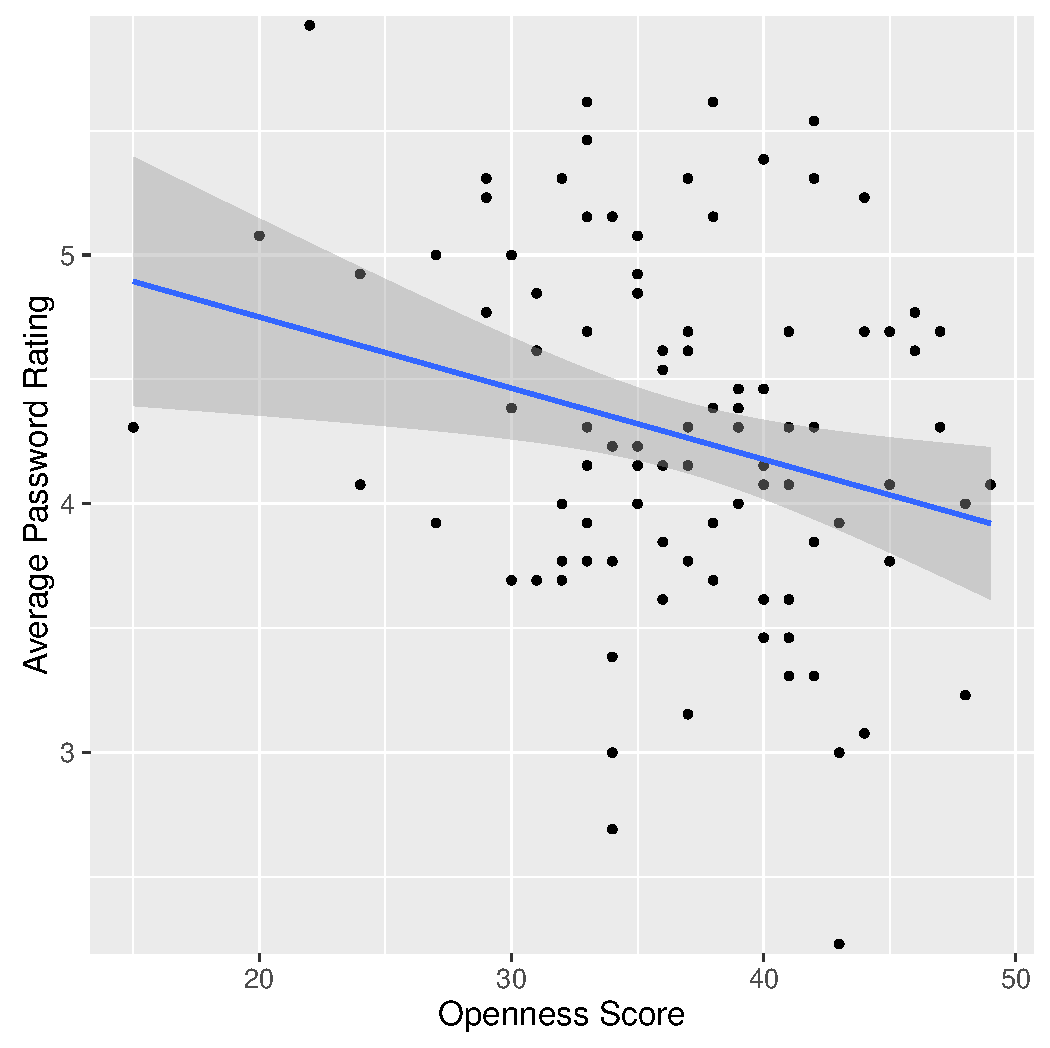
\includegraphics[width=\linewidth]{figures/Openness-ScatterPlot3}
	\caption{\label{fig:openness-scatterplot} Scatter plot of openness scores on x-axis and overall password ratings on y-axis, with fitted regression line and 95\% confidence interval. Participants scoring high on openness are a little more pessimistic in rating the strength of passwords.}
\end{figure}

%%%%%%%%%%%%%%%%%%%%%%%%%%
%%% 
%%% 		STRENGTH COMPARISON
%%% 
%%%%%%%%%%%%%%%%%%%%%%%%%%
\subsubsection{Comparisons Between Two Passwords}
We explored whether personality traits or decision making style influence how participants compare two given passwords. The regression model for the corresponding analysis is shown in Table \ref{tab:Comparison-Regression}. Here, we can see that conscientiousness was retained as predictor in all models. The most interesting association was found when one of the two passwords contained digits: With a rising number of digits, the conscientious participants favored these passwords ($\beta = 0.47, p < 0.01$), but they did not take length into account as often ($\beta = -0.12, ns$). The opposite is true for participants scoring high on the openness scale. They are more likely to vote for the longer password ($\beta = 0.27, p < 0.05$) than for the one containing digits ($\beta = -0.23, p < 0.05$). 

We also see moderate associations between decision making style and the evaluation based on length and strength as measured by zxcvbn. There is a noteworthy finding concerning people ranking high on rational or intuitive decision making style. We find that rational decision makers were worse at identifying the stronger password ($\beta = -0.35, p < 0.01$) than the intuitive decision makers ($\beta = -0.18, ns$).  

We found weak associations between the control variables and password strength assessment, mostly originating from gender or computer-science background. In the comparison task, male participants were more likely to prefer the password consisting of more character classes ($\beta = 0.21, p < 0.05$). 

In all the models, the predictive power was moderate, with an average $R^2_{adj}$ value of $0.13~(SD=0.04)$. However, the model fit was much better than before, when passwords had to be rated without a point of reference. We see that for the comparison, openness was again an important predictor, but conscientiousness was even more important. The associations between GDMS and password comparisons form a diverse spectrum with no evident pattern. 

%regression comparison

% Table generated by Excel2LaTeX from sheet 'Latex Separate Regressions'
\begin{table*}[h]
 \centering
 \small
  \caption{Regression analysis of the comparison task. Conscientiousness and openness are the most important predictors. Open participants were more likely to vote for the longer password instead of the one with digits, while the inverse is true for conscientious participants. Rational decision makers failed to identify the stronger password more often.}
             \begin{tabular}{rl|rr|rrrr}
      & Predictor & \multicolumn{1}{l}{Length} & \multicolumn{1}{l|}{Strength} & \multicolumn{1}{l}{Symbols} & \multicolumn{1}{l}{Digits} & \multicolumn{1}{l}{Cases} & \multicolumn{1}{l}{Classes} \\
\cmidrule{3-8}    \rowcolor[rgb]{ .718,  .871,  .91} \multicolumn{1}{l}{Big Five} & Neuroticism & \cellcolor[rgb]{ 1,  1,  1}  & \cellcolor[rgb]{ .98,  .627,  .459} -0.15 & \cellcolor[rgb]{ 1,  1,  1}  & \cellcolor[rgb]{ .878,  .89,  .514} 0.19 & \cellcolor[rgb]{ 1,  1,  1}  & \cellcolor[rgb]{ 1,  1,  1}  \\
    \rowcolor[rgb]{ .718,  .871,  .91}   & Extraversion & \cellcolor[rgb]{ 1,  1,  1}  & \cellcolor[rgb]{ .98,  .596,  .455} -0.18 & \cellcolor[rgb]{ 1,  1,  1}  & \cellcolor[rgb]{ 1,  1,  1}  & \cellcolor[rgb]{ 1,  1,  1}  & \cellcolor[rgb]{ 1,  1,  1}  \\
    \rowcolor[rgb]{ .718,  .871,  .91}   & Openness & \cellcolor[rgb]{ .741,  .847,  .506} \textbf{0.27} & \cellcolor[rgb]{ .914,  .898,  .514} 0.17 & \cellcolor[rgb]{ 1,  1,  1}  & \cellcolor[rgb]{ .976,  .541,  .443} \textbf{-0.23} & \cellcolor[rgb]{ 1,  1,  1}  & \cellcolor[rgb]{ .984,  .671,  .467} -0.11 \\
    \rowcolor[rgb]{ .718,  .871,  .91}   & Agreeableness & \cellcolor[rgb]{ .969,  .914,  .518} 0.14 & \cellcolor[rgb]{ .996,  .91,  .514} 0.11 & \cellcolor[rgb]{ 1,  1,  1}  & \cellcolor[rgb]{ 1,  1,  1}  & \cellcolor[rgb]{ 1,  1,  1}  & \cellcolor[rgb]{ 1,  1,  1}  \\
    \rowcolor[rgb]{ .718,  .871,  .91}   & Conscientiousness & \cellcolor[rgb]{ .984,  .659,  .467} -0.12 & \cellcolor[rgb]{ .898,  .894,  .514} 0.18 & \cellcolor[rgb]{ .969,  .914,  .518} 0.14 & \cellcolor[rgb]{ .388,  .745,  .482} \textbf{0.47} & \cellcolor[rgb]{ .878,  .89,  .514} 0.19 & \cellcolor[rgb]{ .635,  .816,  .498} \textbf{0.33} \\
    \rowcolor[rgb]{ .988,  .835,  .706} \multicolumn{1}{l}{GDMS} & Rational & \cellcolor[rgb]{ .976,  .486,  .431} \textbf{-0.28} & \cellcolor[rgb]{ .973,  .412,  .42} \textbf{-0.35} & \cellcolor[rgb]{ 1,  1,  1}  & \cellcolor[rgb]{ .898,  .894,  .514} 0.18 & \cellcolor[rgb]{ 1,  1,  1}  & \cellcolor[rgb]{ 1,  1,  1}  \\
    \rowcolor[rgb]{ .988,  .835,  .706}   & Intuitive & \cellcolor[rgb]{ .98,  .627,  .459} -0.15 & \cellcolor[rgb]{ .98,  .596,  .455} -0.18 & \cellcolor[rgb]{ 1,  1,  1}  & \cellcolor[rgb]{ 1,  1,  1}  & \cellcolor[rgb]{ 1,  1,  1}  & \cellcolor[rgb]{ 1,  1,  1}  \\
    \rowcolor[rgb]{ .988,  .835,  .706}   & Dependent & \cellcolor[rgb]{ 1,  1,  1}  & \cellcolor[rgb]{ 1,  1,  1}  & \cellcolor[rgb]{ 1,  1,  1}  & \cellcolor[rgb]{ 1,  1,  1}  & \cellcolor[rgb]{ .984,  .918,  .518} 0.13 & \cellcolor[rgb]{ 1,  1,  1}  \\
    \rowcolor[rgb]{ .988,  .835,  .706}   & Avoidant & \cellcolor[rgb]{ 1,  1,  1}  & \cellcolor[rgb]{ 1,  1,  1}  & \cellcolor[rgb]{ .984,  .659,  .467} -0.12 & \cellcolor[rgb]{ .827,  .875,  .51} 0.22 & \cellcolor[rgb]{ 1,  1,  1}  & \cellcolor[rgb]{ 1,  1,  1}  \\
    \rowcolor[rgb]{ .988,  .835,  .706}   & Spontaneous & \cellcolor[rgb]{ 1,  1,  1}  & \cellcolor[rgb]{ 1,  1,  1}  & \cellcolor[rgb]{ 1,  1,  1}  & \cellcolor[rgb]{ 1,  1,  1}  & \cellcolor[rgb]{ .98,  .616,  .459} -0.16 & \cellcolor[rgb]{ 1,  1,  1}  \\
      & Education &   &   &   & \cellcolor[rgb]{ .984,  .659,  .467} -0.12 &   &  \\
      & CS Background & \cellcolor[rgb]{ .843,  .878,  .51} \textbf{0.21} & \cellcolor[rgb]{ .843,  .878,  .51} \textbf{0.21} &   & \cellcolor[rgb]{ .984,  .682,  .471} -0.1 &   &  \\
      & Male &   &   & \cellcolor[rgb]{ .843,  .878,  .51} \textbf{0.21} & \cellcolor[rgb]{ .949,  .91,  .518} 0.15 & \cellcolor[rgb]{ .706,  .839,  .502} \textbf{0.29} & \cellcolor[rgb]{ .843,  .878,  .51} \textbf{0.21} \\
    \midrule
      & F & 3.95 & 3.78 & 3.37 & 3.13 & 3.86 & 5.75 \\
      & df & 6 & 8 & 3 & 8 & 4 & 3 \\
      & p & \multicolumn{1}{l}{< 0.01} & \multicolumn{1}{l|}{< 0.01} & \multicolumn{1}{l}{< 0.05} & \multicolumn{1}{l}{< 0.01} & \multicolumn{1}{l}{< 0.01} & \multicolumn{1}{l}{<0.01} \\
      & R$^2$ & \cellcolor[rgb]{ .533,  .804,  .608} 0.2 & \cellcolor[rgb]{ .388,  .745,  .482} 0.25 & \cellcolor[rgb]{ .82,  .922,  .855} 0.1 & \cellcolor[rgb]{ .506,  .792,  .584} 0.21 & \cellcolor[rgb]{ .706,  .875,  .757} 0.14 & \cellcolor[rgb]{ .675,  .863,  .729} 0.15 \\
      & Adjusted R$^2$& \cellcolor[rgb]{ .494,  .788,  .576} 0.15 & \cellcolor[rgb]{ .388,  .745,  .482} 0.18 & \cellcolor[rgb]{ .776,  .906,  .82} 0.07 & \cellcolor[rgb]{ .494,  .788,  .576} 0.15 & \cellcolor[rgb]{ .671,  .863,  .729} 0.1 & \cellcolor[rgb]{ .565,  .82,  .635} 0.13 \\
    \bottomrule
    \bottomrule
    \end{tabular}%
  \label{tab:Comparison-Regression}%
\end{table*}%


\subsubsection{Qualitative Findings}
While entering an elaborate response was not mandatory, all but one participant (\textit{n}=99) gave a brief and in most cases comprehensible explanation for their ratings. The numbers do not necessarily add up to \textit{n}, because answers could receive multiple codes.

We identified four overall themes in how the participants approached rating passwords: \textit{Character diversity}, \textit{creation strategy}, \textit{predictability} and \textit{other}. The character diversity code consists of participants mentioning the importance of symbols (69), digits (52), upper-/lowercase letters (45) and general variety of characters (16). Regarding the creation strategy, many participants penalized passwords when they contained actual words (40) or personal information (3). The predictability category was divided into answers referring to character substitutions (10), patterns (17), guessability (12), randomness (20), length (25) and the position of symbols/digits (6). The other themes were established from 8 participants using technical jargon (e.g. ``attack'' or ``brute force'') and those who identified the obfuscated passwords (2). 

\subsubsection{Synthesis}
We found that participants evaluate password strength by looking for specific patterns. Regression models and qualitative analysis show that respondents mostly penalized lack of diversity and randomness which is consistent with the related work \cite{Ur2016PerceptionsPassword}. Thus, the associations originating from different personality types or decision making style were small in many cases, but not negligible. The education level was generally insignificant regarding the strength evaluation. However, technical background and gender played a role in the comparison task, because male participants were more likely influenced by character variety. The predictive power of the independent variables was higher in the comparison task than in the standalone rating. The most important factors were \textbf{openness} on \textbf{conscientiousness} from the Big-Five model, and \textbf{rationality} from the GDMS. 

%%%%%%%%%%%%%%%%%%%%%%%%%%%%%%%%%%%%%%%%%%%
%%%%
%%%%
%%%%			STUDY  3 THREE DREI
%%%%			SELECTION
%%%%
%%%%
%%%%%%%%%%%%%%%%%%%%%%%%%%%%%%%%%%%%%%%%%%%
\section{Study 3: Password Selection}
% ALINE
% GOALS
As a final step in our ``password personality'' exploration, we ran an online survey. Having investigated preferences for policies and the perception of passwords, the main goal of the third study was to evaluate potential associations between personality and password \textit{selection}. To overcome some of the limitations of the previous study, we hoped to increase the sample size and reduce the number of items during the study. Moreover, further answers about the participants' explanations and motivations were considered to better understand the weight of personality factors. We determined the following research questions: 1) Are there correlations between password features (topology) and personality traits? 2) Do certain facets of personality shine through in password management behavior, e.g. the tendency to write down passwords?

\subsection{Procedure and Tools}
The study was designed to take no more than ten minutes. The briefing page informed participants about the purpose of the study and data disclosure policies. After acknowledging the conditions of participation, respondents were asked to create a password. To boost ecological validity, we provided a fictitious but realistic scenario \cite{Komanduri2011OfPasswordsAndPeople}. The task was to come up with a new password for a new email account that they were going to use as their main address. Further, the instruction pointed out that the incentive would only be paid of if the participants chose a password they could recall later on. A \textit{basic8} policy was enforced, as it is one of the most representative policies in the wild (see chapter \ref{chap:policies_reuse}). This loose policy would also allow for both very complex and rather simple passwords, which could be associated with personality traits. Having successfully confirmed the password, respondents were taken to a questionnaire about demographics, just like in the first two studies. 

Next, participants completed the BFI-K questionnaire consisting of 21 items that have to be rated on a 5-point scale. We opted not to use the 50-item inventory for the sake of saving time. We added an item that served as an attention check. It asked to respond to this item with ``disagree''. Failure to follow this instruction allowed us to drop the response from the dataset. The resulting 22 items were shuffled to avoid sequence effects. 

Afterwards, we surveyed respondents about their password management behaviors and preferences. We used multiple-choice and open responses to collect qualitative, self-reported data. For instance, we wanted to know how they cope with multiple accounts or how they reuse passwords. The survey concluded with a recall task, where participants provided their initially chosen password. They could try as often as they liked, and the number of attempts were recorded. In case they were unable to recall their password, they could proceed anyhow and take part in the lottery. If they chose to provide an email address in the final step, this data was stored separately from the questionnaire data to avoid privacy issues. 

\subsection{Recruitment and Sample}
Participants were invited via a university newsletter, and snowballing the link via personal connections and posts on social networks. The questionnaire was in German and participants were screened about their command of the German language. We instructed participants to take the survey on a desktop. 
%TODO aline says 184 but the data set is smaller :-/ ?
%all the following numbers are from the smaller data set.
184 people completed the survey, but we had to drop the responses of 8 participants because their reponse timings were too unrealistic. From the 176 remaining respondents, 89 were male, 86 female and 1 preferred not to answer. 116 were students, i.e. a rather high proportion (66\%). Consequently, the average age was 25 years (range [16;55], $SD$=6, $Md$= 24). 67 (38\%) reportedly had an IT-background. 129 respondents chose to participate in the raffle for shopping vouchers. 

\subsection{Limitations}
\todo{Password selection not realistic / attention check item was badly placed and not well explained. 30 feedback emails.}

\subsection{Results}
% descriptives
The resulting passwords had a median-length of 10 characters ([8;22]), i.e. many participants went beyond the minimum requirement. Figure \ref{fig:personality:study3:metrics-overview} visualizes additional metrics that show that passwords were stronger than expected. In the following, we try to fit generalized additive models to the data using big-five trait scores as covariates. 

\begin{figure}[tbph]
	\centering
	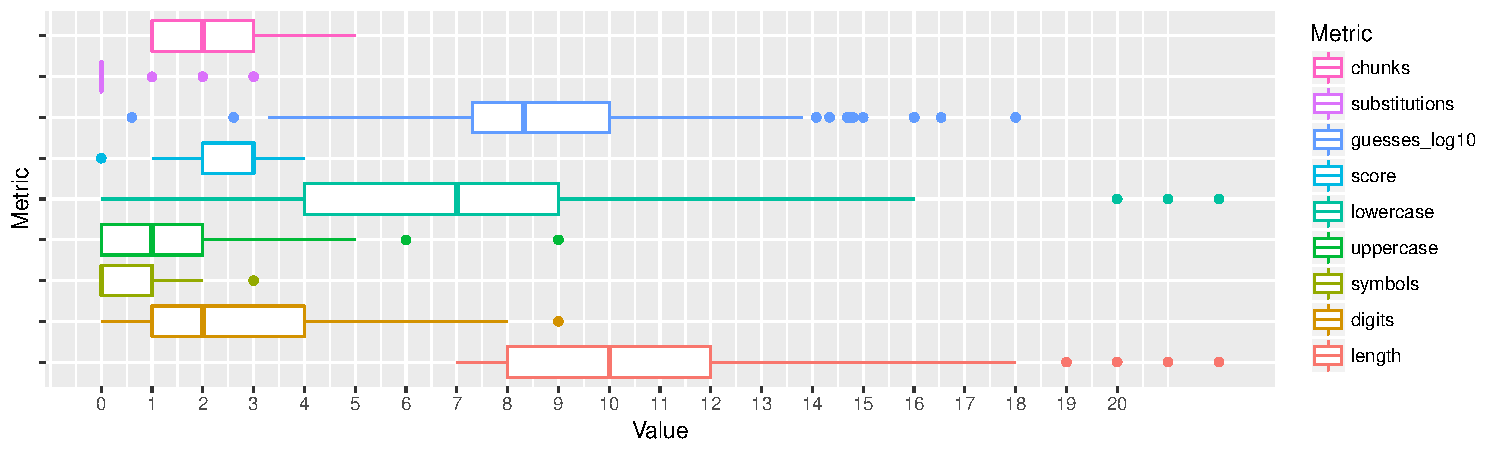
\includegraphics[width=1\linewidth]{figures/personality/study3-metrics-overview}
	\caption{\label{fig:personality:study3:metrics-overview} Zxcvbn metrics for user selected passwords.}
\end{figure}

% maximum R-sq 
\subsubsection{Password Composition}
First, we use zxcvbn metrics as response variables, i.e. we explore marginal associations from big five traits. As before, we include age, gender and IT-background as control covariates. 

\subsubsection{Memorability}


\subsection{Password Management Strategies}
% binary -- logit model ``write down'': yes no

\subsection{Learnings}


%%%%%%%%%%%%%%%%%%%%%%%%%%%%%%%%%%%%%%%%%%%
%%%%
%%%%
%%%%			GENERAL DISCUSSION
%%%%
%%%%%%%%%%%%%%%%%%%%%%%%%%%%%%%%%%%%%%%%%%%
\section{Discussion and Implications}
%In this section we interpret the results and hope to shed light on potential explanations for their origins. % and show the implications for password-authentication systems.

%TODO more elaborately discuss the origin of the results.
% Table generated by Excel2LaTeX from sheet 'Personality Overview'
\begin{table}[tbp]
  \centering
  \caption{\label{tab:personality:associations-overview}
  	Overview of significant associations between Big-Five traits, control factors, and different metrics across three studies. Arrows indicate direction of the associations, colors also highlight significance levels (red/ocher: $p$ < 0.05/0.1 negative assoc., greens: $p$ < 0.001/0.01/0.05/0.1 positive assoc.) Openness and Conscientiousness are the most important factors from the Big-Five model, and having an IT background was an indispensable control factor.
  }\resizebox{\linewidth}{!}{
    \begin{tabular}{p{6.5cm}rp{0.8cm}rrrrrrrr}
    \rowcolor[rgb]{ .38,  .612,  1} \textcolor[rgb]{ 1,  1,  1}{\textbf{Metric}} & \multicolumn{1}{l}{\textcolor[rgb]{ 1,  1,  1}{\textbf{Type}}} & \multicolumn{1}{p{0.8cm}|}{\textcolor[rgb]{ 1,  1,  1}{\textbf{Study}}} & \multicolumn{1}{c}{\textcolor[rgb]{ 1,  1,  1}{\textbf{O}}} & \multicolumn{1}{c}{\textcolor[rgb]{ 1,  1,  1}{\textbf{C}}} & \multicolumn{1}{c}{\textcolor[rgb]{ 1,  1,  1}{\textbf{E}}} & \multicolumn{1}{c}{\textcolor[rgb]{ 1,  1,  1}{\textbf{A}}} & \multicolumn{1}{c|}{\textcolor[rgb]{ 1,  1,  1}{\textbf{N}}} & \multicolumn{1}{l}{\textcolor[rgb]{ 1,  1,  1}{\textbf{Age}}} & \multicolumn{1}{l}{\textcolor[rgb]{ 1,  1,  1}{\textbf{Gender}}} & \multicolumn{1}{l}{\textcolor[rgb]{ 1,  1,  1}{\textbf{IT}}} \\
    
    Difficulty to create 2word12 PW & \multicolumn{1}{l}{Usability} & \multicolumn{1}{r|}{1} &       &       &       &       & \multicolumn{1}{r|}{} &       & \multicolumn{1}{l}{\cellcolor[rgb]{ .486,  .682,  0} \textcolor[rgb]{ 1,  1,  1}{\emoji{2197} (< .1)}} &  \\

    Difficulty to create 1emoji12 PW & \multicolumn{1}{l}{Usability} & \multicolumn{1}{r|}{1} &       &       &       & \multicolumn{1}{l}{\cellcolor[rgb]{ .871,  .549,  0} \textcolor[rgb]{ 1,  1,  1}{\emoji{2198} (< .1)}} & \multicolumn{1}{l|}{\cellcolor[rgb]{ .973,  .463,  .427} \textcolor[rgb]{ 1,  1,  1}{\emoji{2198} (< .05)}} &       & \multicolumn{1}{l}{\cellcolor[rgb]{ .486,  .682,  0} \textcolor[rgb]{ 1,  1,  1}{\emoji{2197} (< .1)}} &  \\
    
    Preference of 3class12 policy & \multicolumn{1}{l}{Attitude} & \multicolumn{1}{r|}{1} &       &       &       & \multicolumn{1}{l}{\cellcolor[rgb]{ .973,  .463,  .427} \textcolor[rgb]{ 1,  1,  1}{\emoji{2198} (< .05)}} & \multicolumn{1}{r|}{} &       &       &  \\
    
    Preference of 2word12 policy & \multicolumn{1}{l}{Attitude} & \multicolumn{1}{r|}{1} &       &       & \multicolumn{1}{l}{\cellcolor[rgb]{ .973,  .463,  .427} \textcolor[rgb]{ 1,  1,  1}{\emoji{2198} (< .05)}} &       & \multicolumn{1}{r|}{} &       &       &  \\
    
    Preference of 1emoji12 policy & \multicolumn{1}{l}{Attitude} & \multicolumn{1}{r|}{1} &       &       &       & \multicolumn{1}{l}{\cellcolor[rgb]{ 0,  .729,  .22} \textcolor[rgb]{ 1,  1,  1}{\emoji{2197} (< .05)}} & \multicolumn{1}{l|}{\cellcolor[rgb]{ .486,  .682,  0} \textcolor[rgb]{ 1,  1,  1}{\emoji{2197} (< .1)}} &       &       & \multicolumn{1}{l}{\cellcolor[rgb]{ .973,  .463,  .427} \textcolor[rgb]{ 1,  1,  1}{\emoji{2198} (< .05)}} \\
    
    Time to create PW & \multicolumn{1}{l}{Usability} & \multicolumn{1}{r|}{1} &       & \multicolumn{1}{l}{\cellcolor[rgb]{ .973,  .463,  .427} \textcolor[rgb]{ 1,  1,  1}{\emoji{2198} (< .05)}} &       &       & \multicolumn{1}{l|}{\cellcolor[rgb]{ .871,  .549,  0} \textcolor[rgb]{ 1,  1,  1}{\emoji{2198} (< .1)}} &       & \multicolumn{1}{l}{\cellcolor[rgb]{ 0,  .753,  .545} \textcolor[rgb]{ 1,  1,  1}{\emoji{2197} (< .01)}} &  \\
    \midrule
    
    Overall tendency to judge PWs & \multicolumn{1}{l}{Behavior} & \multicolumn{1}{r|}{2} & \multicolumn{1}{l}{\cellcolor[rgb]{ .973,  .463,  .427} \textcolor[rgb]{ 1,  1,  1}{\emoji{2198} (< .05)}} &       &       &       & \multicolumn{1}{r|}{} &       &       &  \\
    
    Comparing PWs based on complexity & \multicolumn{1}{l}{Behavior} & \multicolumn{1}{r|}{2} &       & \multicolumn{1}{l}{\cellcolor[rgb]{ 0,  .753,  .545} \textcolor[rgb]{ 1,  1,  1}{\emoji{2197} (< .01)}} &       &       & \multicolumn{1}{r|}{} &       & \multicolumn{1}{l}{\cellcolor[rgb]{ .973,  .463,  .427} \textcolor[rgb]{ 1,  1,  1}{\emoji{2198} (< .05)}} &  \\
    
    Comparing PWs based on digits & \multicolumn{1}{l}{Behavior} & \multicolumn{1}{r|}{2} & \multicolumn{1}{l}{\cellcolor[rgb]{ .973,  .463,  .427} \textcolor[rgb]{ 1,  1,  1}{\emoji{2198} (< .05)}} & \multicolumn{1}{l}{\cellcolor[rgb]{ 0,  .749,  .769} \textcolor[rgb]{ 1,  1,  1}{\emoji{2197} (< .001)}} &       &       & \multicolumn{1}{r|}{} &       &       &  \\
    
    Comparing PWs based on uppercase & \multicolumn{1}{l}{Behavior} & \multicolumn{1}{r|}{2} &       & \multicolumn{1}{l}{\cellcolor[rgb]{ .486,  .682,  0} \textcolor[rgb]{ 1,  1,  1}{\emoji{2197} (< .1)}} &       &       & \multicolumn{1}{r|}{} & \multicolumn{1}{l}{\cellcolor[rgb]{ .871,  .549,  0} \textcolor[rgb]{ 1,  1,  1}{\emoji{2198} (< .1)}} &       &  \\
    
    Comparing PWs based on length & \multicolumn{1}{l}{Behavior} & \multicolumn{1}{r|}{2} & \multicolumn{1}{l}{\cellcolor[rgb]{ 0,  .729,  .22} \textcolor[rgb]{ 1,  1,  1}{\emoji{2197} (< .05)}} & \multicolumn{1}{l}{\cellcolor[rgb]{ .973,  .463,  .427} \textcolor[rgb]{ 1,  1,  1}{\emoji{2198} (< .05)}} &       &       & \multicolumn{1}{r|}{} & \multicolumn{1}{l}{ } &       & \multicolumn{1}{l}{\cellcolor[rgb]{ 0,  .729,  .22} \textcolor[rgb]{ 1,  1,  1}{\emoji{2197} (< .05)}} \\
    \midrule
    
    Length of created PW & \multicolumn{1}{l}{Behavior} & \multicolumn{1}{r|}{3} &       &       &       &       & \multicolumn{1}{l|}{\cellcolor[rgb]{ 0,  .729,  .22} \textcolor[rgb]{ 1,  1,  1}{\emoji{2197} (< .05)}} &       &       & \multicolumn{1}{l}{\cellcolor[rgb]{ 0,  .729,  .22} \textcolor[rgb]{ 1,  1,  1}{\emoji{2197} (< .05)}} \\
    
    Guess number of created PW & \multicolumn{1}{l}{Behavior} & \multicolumn{1}{r|}{3} &       &       &       &       & \multicolumn{1}{r|}{} &       &       & \multicolumn{1}{l}{\cellcolor[rgb]{ 0,  .729,  .22} \textcolor[rgb]{ 1,  1,  1}{\emoji{2197} (< .05)}} \\
    
    zxcvbn score of created PW & \multicolumn{1}{l}{Behavior} & \multicolumn{1}{r|}{3} &       &       &       &       & \multicolumn{1}{l|}{\cellcolor[rgb]{ .486,  .682,  0} \textcolor[rgb]{ 1,  1,  1}{\emoji{2197} (< .1)}} &       &       & \multicolumn{1}{l}{\cellcolor[rgb]{ 0,  .729,  .22} \textcolor[rgb]{ 1,  1,  1}{\emoji{2197} (< .05)}} \\
    
    Created PW is passphrase & \multicolumn{1}{l}{Behavior} & \multicolumn{1}{r|}{3} &       &       &       &       & \multicolumn{1}{r|}{} &       &       & \multicolumn{1}{l}{\cellcolor[rgb]{ 0,  .729,  .22} \textcolor[rgb]{ 1,  1,  1}{\emoji{2197} (< .05)}} \\
    
    Created PW is random & \multicolumn{1}{l}{Behavior} & \multicolumn{1}{r|}{3} &       &       &       &       & \multicolumn{1}{r|}{} &       & \multicolumn{1}{l}{\cellcolor[rgb]{ .973,  .463,  .427} \textcolor[rgb]{ 1,  1,  1}{\emoji{2198} (< .05)}} & \multicolumn{1}{l}{\cellcolor[rgb]{ .871,  .549,  0} \textcolor[rgb]{ 1,  1,  1}{\emoji{2198} (< .1)}} \\
    
    Cope by memorizing PW & \multicolumn{1}{l}{Behavior} & \multicolumn{1}{r|}{3} &       & \multicolumn{1}{l}{\cellcolor[rgb]{ .871,  .549,  0} \textcolor[rgb]{ 1,  1,  1}{\emoji{2198} (< .1)}} & \multicolumn{1}{l}{\cellcolor[rgb]{ 0,  .729,  .22} \textcolor[rgb]{ 1,  1,  1}{\emoji{2197} (< .05)}} & \multicolumn{1}{l}{\cellcolor[rgb]{ .871,  .549,  0} \textcolor[rgb]{ 1,  1,  1}{\emoji{2198} (< .1)}} & \multicolumn{1}{r|}{} & \multicolumn{1}{l}{\cellcolor[rgb]{ .871,  .549,  0} \textcolor[rgb]{ 1,  1,  1}{\emoji{2198} (< .1)}} &       & \multicolumn{1}{l}{\cellcolor[rgb]{ .973,  .463,  .427} \textcolor[rgb]{ 1,  1,  1}{\emoji{2198} (< .05)}} \\
    
    Cope by reusing PW & \multicolumn{1}{l}{Behavior} & \multicolumn{1}{r|}{3} &       &       &       & \multicolumn{1}{l}{\cellcolor[rgb]{ .871,  .549,  0} \textcolor[rgb]{ 1,  1,  1}{\emoji{2198} (< .1)}} & \multicolumn{1}{r|}{} &       &       & \multicolumn{1}{l}{\cellcolor[rgb]{ .973,  .463,  .427} \textcolor[rgb]{ 1,  1,  1}{\emoji{2198} (< .05)}} \\
    
    Cope by using PWM & \multicolumn{1}{l}{Behavior} & \multicolumn{1}{r|}{3} & \multicolumn{1}{l}{\cellcolor[rgb]{ .973,  .463,  .427} \textcolor[rgb]{ 1,  1,  1}{\emoji{2198} (< .05)}} &       &       &       & \multicolumn{1}{r|}{} &       & \multicolumn{1}{l}{\cellcolor[rgb]{ .871,  .549,  0} \textcolor[rgb]{ 1,  1,  1}{\emoji{2198} (< .1)}} & \multicolumn{1}{l}{\cellcolor[rgb]{ 0,  .729,  .22} \textcolor[rgb]{ 1,  1,  1}{\emoji{2197} (< .05)}} \\
    
    Cope by using paper / files & \multicolumn{1}{l}{Behavior} & \multicolumn{1}{r|}{3} &       &       & \multicolumn{1}{l}{\cellcolor[rgb]{ .973,  .463,  .427} \textcolor[rgb]{ 1,  1,  1}{\emoji{2198} (< .05)}} &       & \multicolumn{1}{r|}{} &       &       &  \\
    \midrule
    \midrule
    %\textbf{Number of significant associations (p < 0.05)} &       &       & \textbf{4} & \textbf{4} & \textbf{3} & \textbf{2} & \textbf{2} & \textbf{0} & \textbf{2} & \textbf{8} \\
    \multicolumn{3}{l}{\textbf{Number of significant associations (p < 0.05 [0.1] )}} & \textbf{4~[4]} & \textbf{4~[6]} & \textbf{3~[3]} & \textbf{2~[5]} & \textbf{2~[5]} & \textbf{0~[2]} & \textbf{3~[6]} & \textbf{9~[9]} \\
    \end{tabular}%
}
\end{table}%
%tab:personality:associations-overview

% Egelman says:
\subsection{Overarching Themes and User Segments}
Egelman and Peer highlighted the importance of the the question \textit{which psychographic segments should be targeted [in security and privacy mitigations]?} While they focused on their newly developed SeBIS scale and other psychometric constructs, we are able to give new pointers for segmenting users based on their Big-Five traits in conjunction with demographic factors. To approach the segmentation, we can look at the overall influences of personality and demographic factors on different metrics. Table \ref{tab:personality:associations-overview} lists all significant marginal associations from all three studies. 

% Neuroticism
\paragraph{Neuroticism} In study 1, the primary observation was that neuroticism was associated with difficulty to create an emoji password. Neuroticism was not associated with any perception metric in study 2, but the third study revealed an interesting association between neuroticsm and self-selected passwords. Metrics in the first and the third study revolve around password \textit{creation}: It appears to be both \textbf{easier} to find a password expressing emotions for participants scoring high on neuroticism, and their passwords turned out significantly \textbf{longer} in the third study. 
% story: ``I see the benefit of creating stronger passwords, and I don't mind adding something I like to memorize them, so emojis inside passwords might be cool.''
Thus, targeting neuroticism with persuasive interventions during password creation might boost these positive associations. Nudges should thus focus on making emotional state more \textit{salient} and point out benefits of password length to \textit{positively reinforce} this behavior. 

% Openness
\paragraph{Openness} The usability of different composition policies was not associated with openness, but the perception of password strength showed conclusive associations in that passwords were generally judged \textbf{weaker} with higher openness scores. Participants strongly showing the openness trait were also more likely to base their decision on \textbf{password length} rather than the number of digits. In study 3, we observed that coping strategies involving a password manager were \textbf{less likely} to be found with participants with high openness scores. 
% paraphrased story: ``your passwords are weak, mine are stronger, because they are longer and I don't need help remembering them!''
The significant associations, and absence thereof, tell a conclusive story if we look at passphrases and mnemonic phrase-based passwords. Those types of passwords are strong and often not overly complex \cite{Keith2009PassphraseDesign,Kuo2006HumanSelectionMnemonic,Shay2012CorrectHorseBatteryStaple}. Passphrases, for instance, are a technique to facilitate memorization. They also easily exceed length requirements. If they consist of uppercase and lowercase letters, and are separated with regular punctuation symbols, there is no need to add digits to meet a three-class requirement: the passphrase is already complex enough. All this is visible in the study behavior of participants scoring high on openness, despite the absence of associations between openness and the type of created password in study 3. 

% Conscientiousness
\paragraph{Conscientiousness} Like openness, conscientiousness was a major factor in study 2. There was evidence that participants, who strongly show this trait, tend to believe a more \textbf{complex} password is better than a long password. We could explain this finding by looking at the attributes that are usually found with conscientious people: diligence and neatness. Following password rules requires these facets to ensure a strong outcome. The results in study 1 (less time taken to create a password) and study 3 (slight tendency to refrain from memorizing passwords) are harder to interpret. We could expect that crafting a strong memorable password takes due diligence and more time, thus the shorter time spent by conscientious participants is counterintuitive. Perhaps it is due to the measurement approach in our study. We started taking the time as soon as the password field was focused and the timing ended when the field lost focus (``blur'' event). It is possible that conscientious participants took their time to reflect on what they wanted to enter into the field, and only then started the task. However, we do not have the data to support this argument.
% story: ``I think a strong password needs to have digits and symbols, then it can be shorter. Dictionary words should not be used.''


% Agreeableness and Extraversion
\paragraph{Agreeableness and Extraversion} Table \ref{tab:personality:associations-overview} shows that agreeableness only showed a conclusive result in study 1. A more demanding policy like 3class12 did not appeal to participants scoring high on agreeableness, while they did favor the emoji-policy much more. Cheerfulness, empathy and cooperation are often characteristics represented by this trait. 
% story: ``hey that's cool, let me see which emoji I can choose to come up with something memorable that matches the constraints and context.'' 
Participants might have favored cheerful emojis to cooperate on finding a suitable solution together. Thus, password selection could have been more fun and thus more pleasing for those participants. Since there was no sign of focusing on password strength, we hypothesize that memorability might be more important for them. 
Regarding extraversion, we found that participants scoring high on this trait disliked a word-based policy and were more likely to memorize passwords than writing them down. This is probably the most difficult result to interpret, because extraversion is a more situationally dependent trait than the four others -- a phenomenon coined as ``ambiversion'' \cite{Grant2013Ambivert}. This could have become visible if our regression models had shown more curvilinear relationships, but those were not significantly more likely for extraversion than for other traits. We therefore refrain from further discussion and note that additional data would be necessary to evaluate the stability of this predictor. 

\paragraph{Demographic Factors}
From Table \ref{tab:personality:associations-overview}, it is evident that associations with the chosen metrics are more likely to be found with demographic variables as predictors. This was especially true for study 3, where almost all outcomes were associated with having experience or education in a computer-science related field. This is an unsurprising finding, because this user group can better judge the implications of their behavior. Nevertheless, the additional factors help us segment user groups in higher detail. 

% Overall picture
\subsubsection{Deriving Segments: Password Personas}\label{sec:personality:personas}
% why do we do this / goals
With the above themes and stories, we are able to derive a number of user segments that can be targeted by security mitigations. Segmentation can inform upcoming research and design directions. For instance, segments serve the generation of hypotheses and play a role in the creation of new psychographic constructs. The ``securing'' dimension of the \gls{SeBIS} might be enriched by user archetypes to \textit{explain} attitudes and behaviors rather than just measuring them. Here, \glspl{persona} constitute a common design tool for segmentation. These fictional users can be targeted in the design of persuasive interventions. From the data of three studies on password personality, and backed up by related work, I created a set of four ``password personas'' that inform design choices in Part \ref{part:design_space} of this thesis. They are shown in Figure \ref{fig:personality:personas}. At this point, the personas still remain abstract to account for the early stage of research about password personality. Personas should be ``living'' templates that are updated based on new data \cite{Gothelf2013LeanUX}. 

\begin{figure}[!htbp]
	\centering
	\fcolorbox{dividergray}{white}{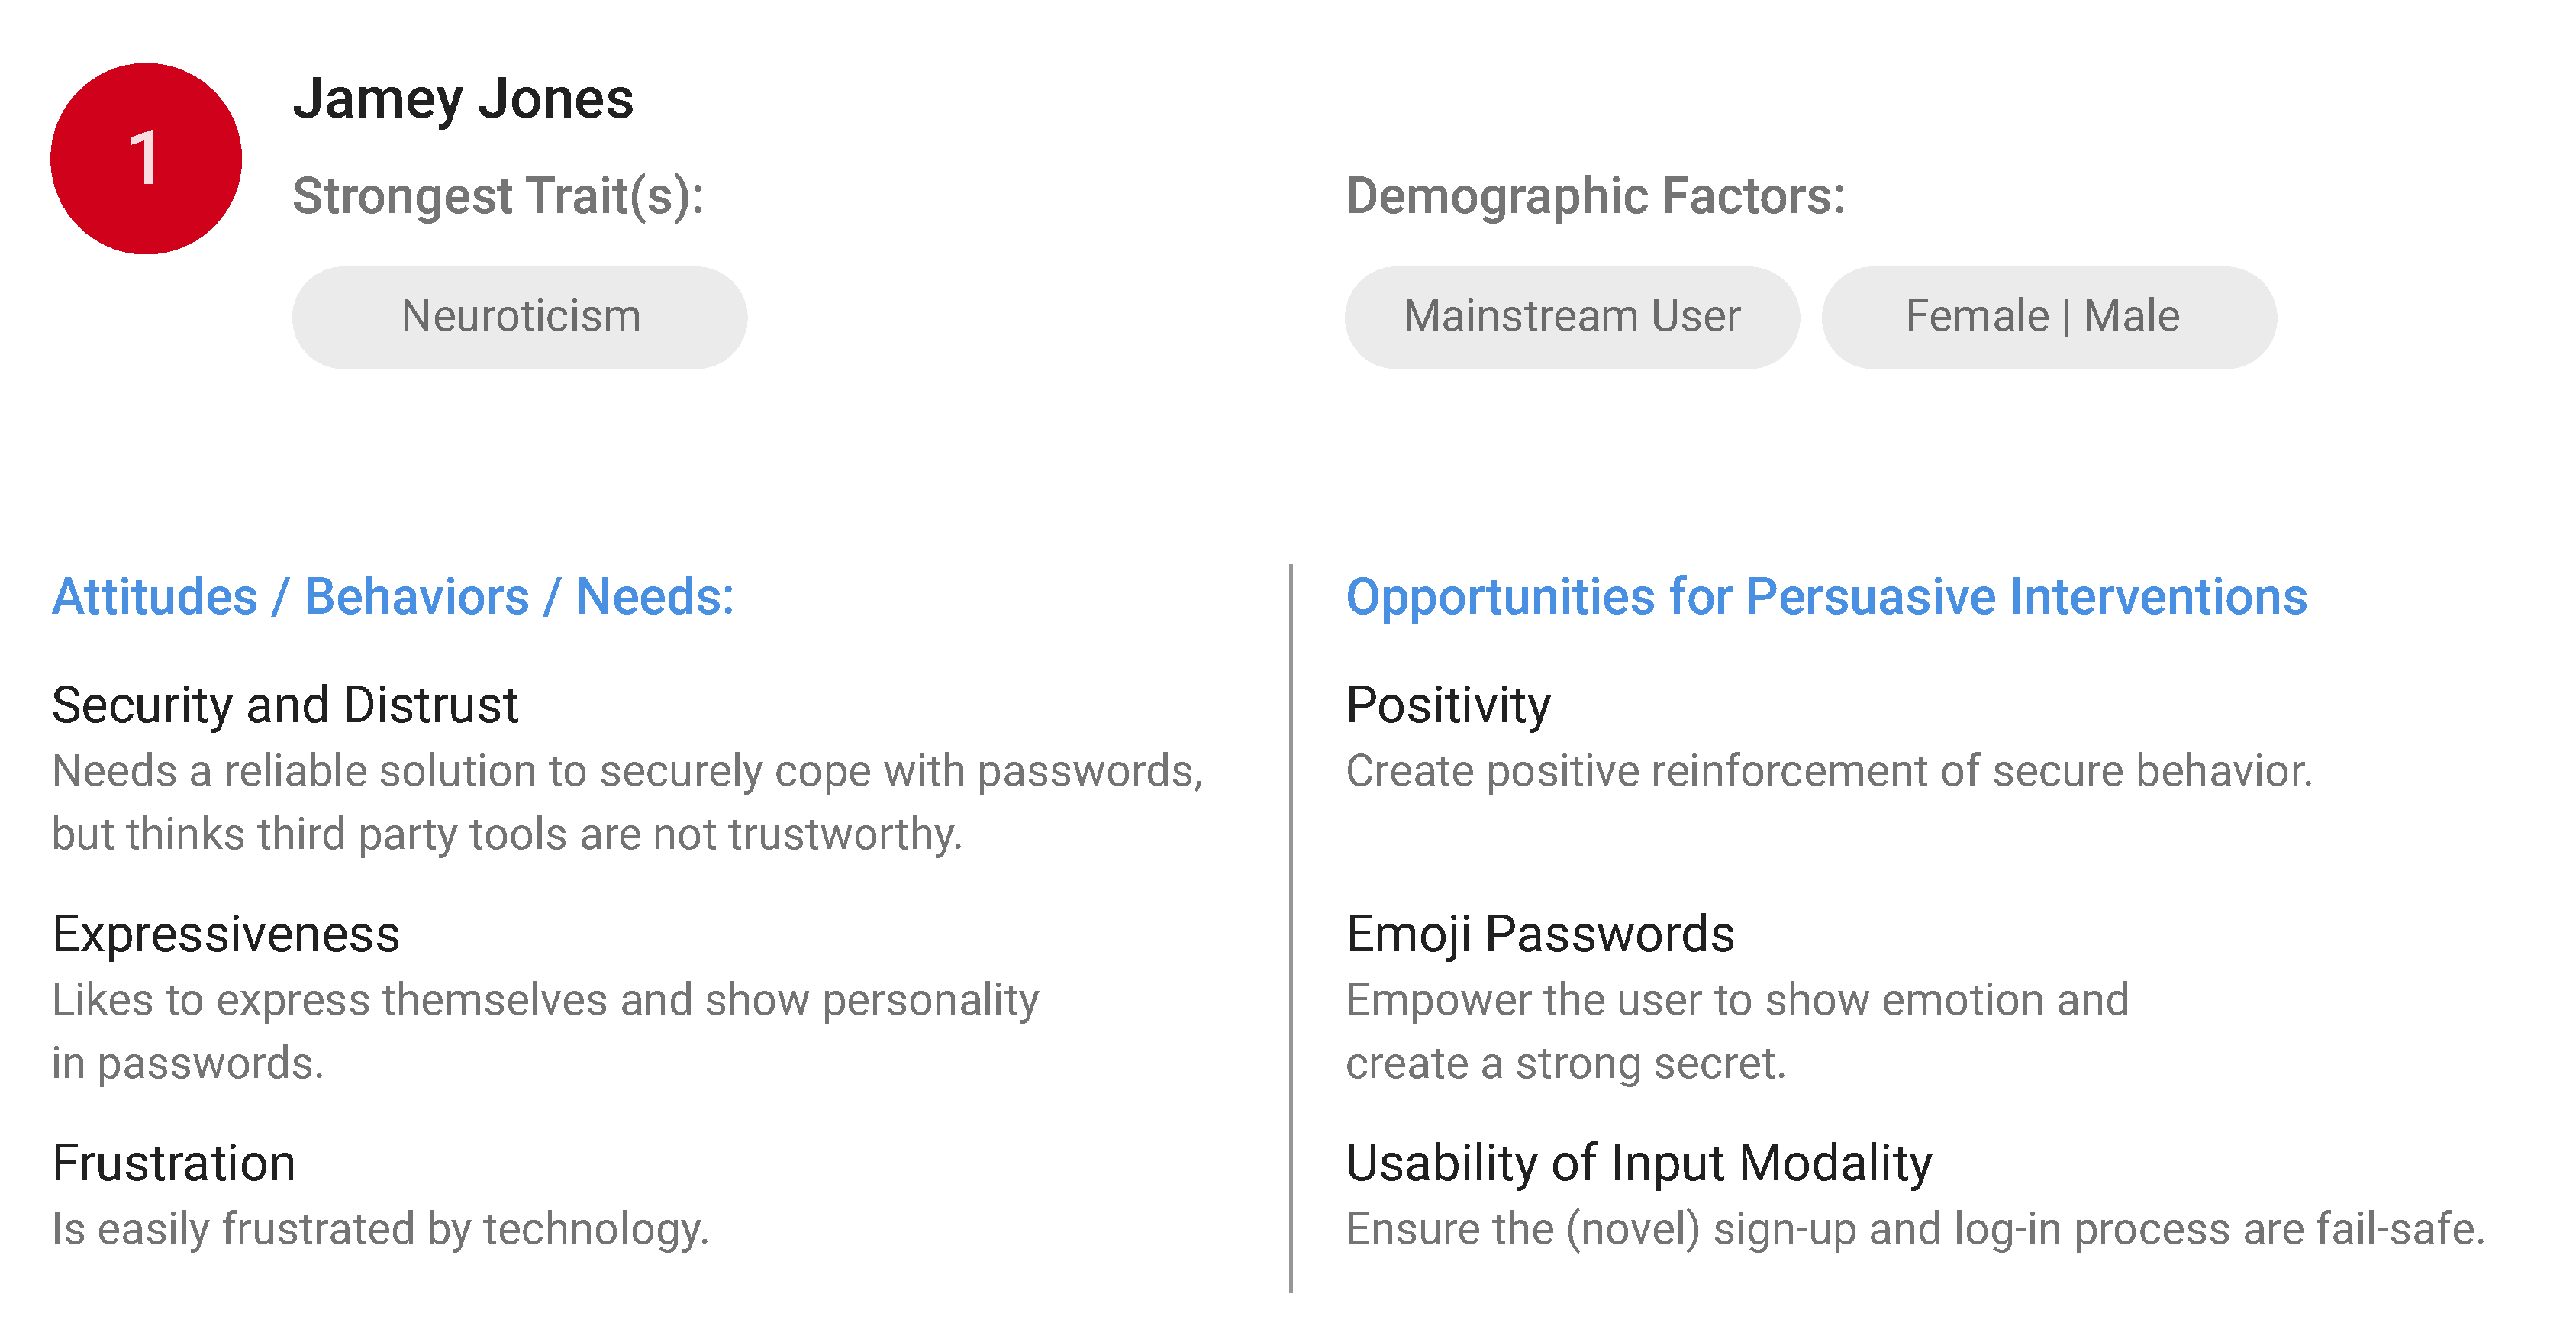
\includegraphics[width=0.7\linewidth]{personality/personas/Neurotic-Persona}}
	\fcolorbox{dividergray}{white}{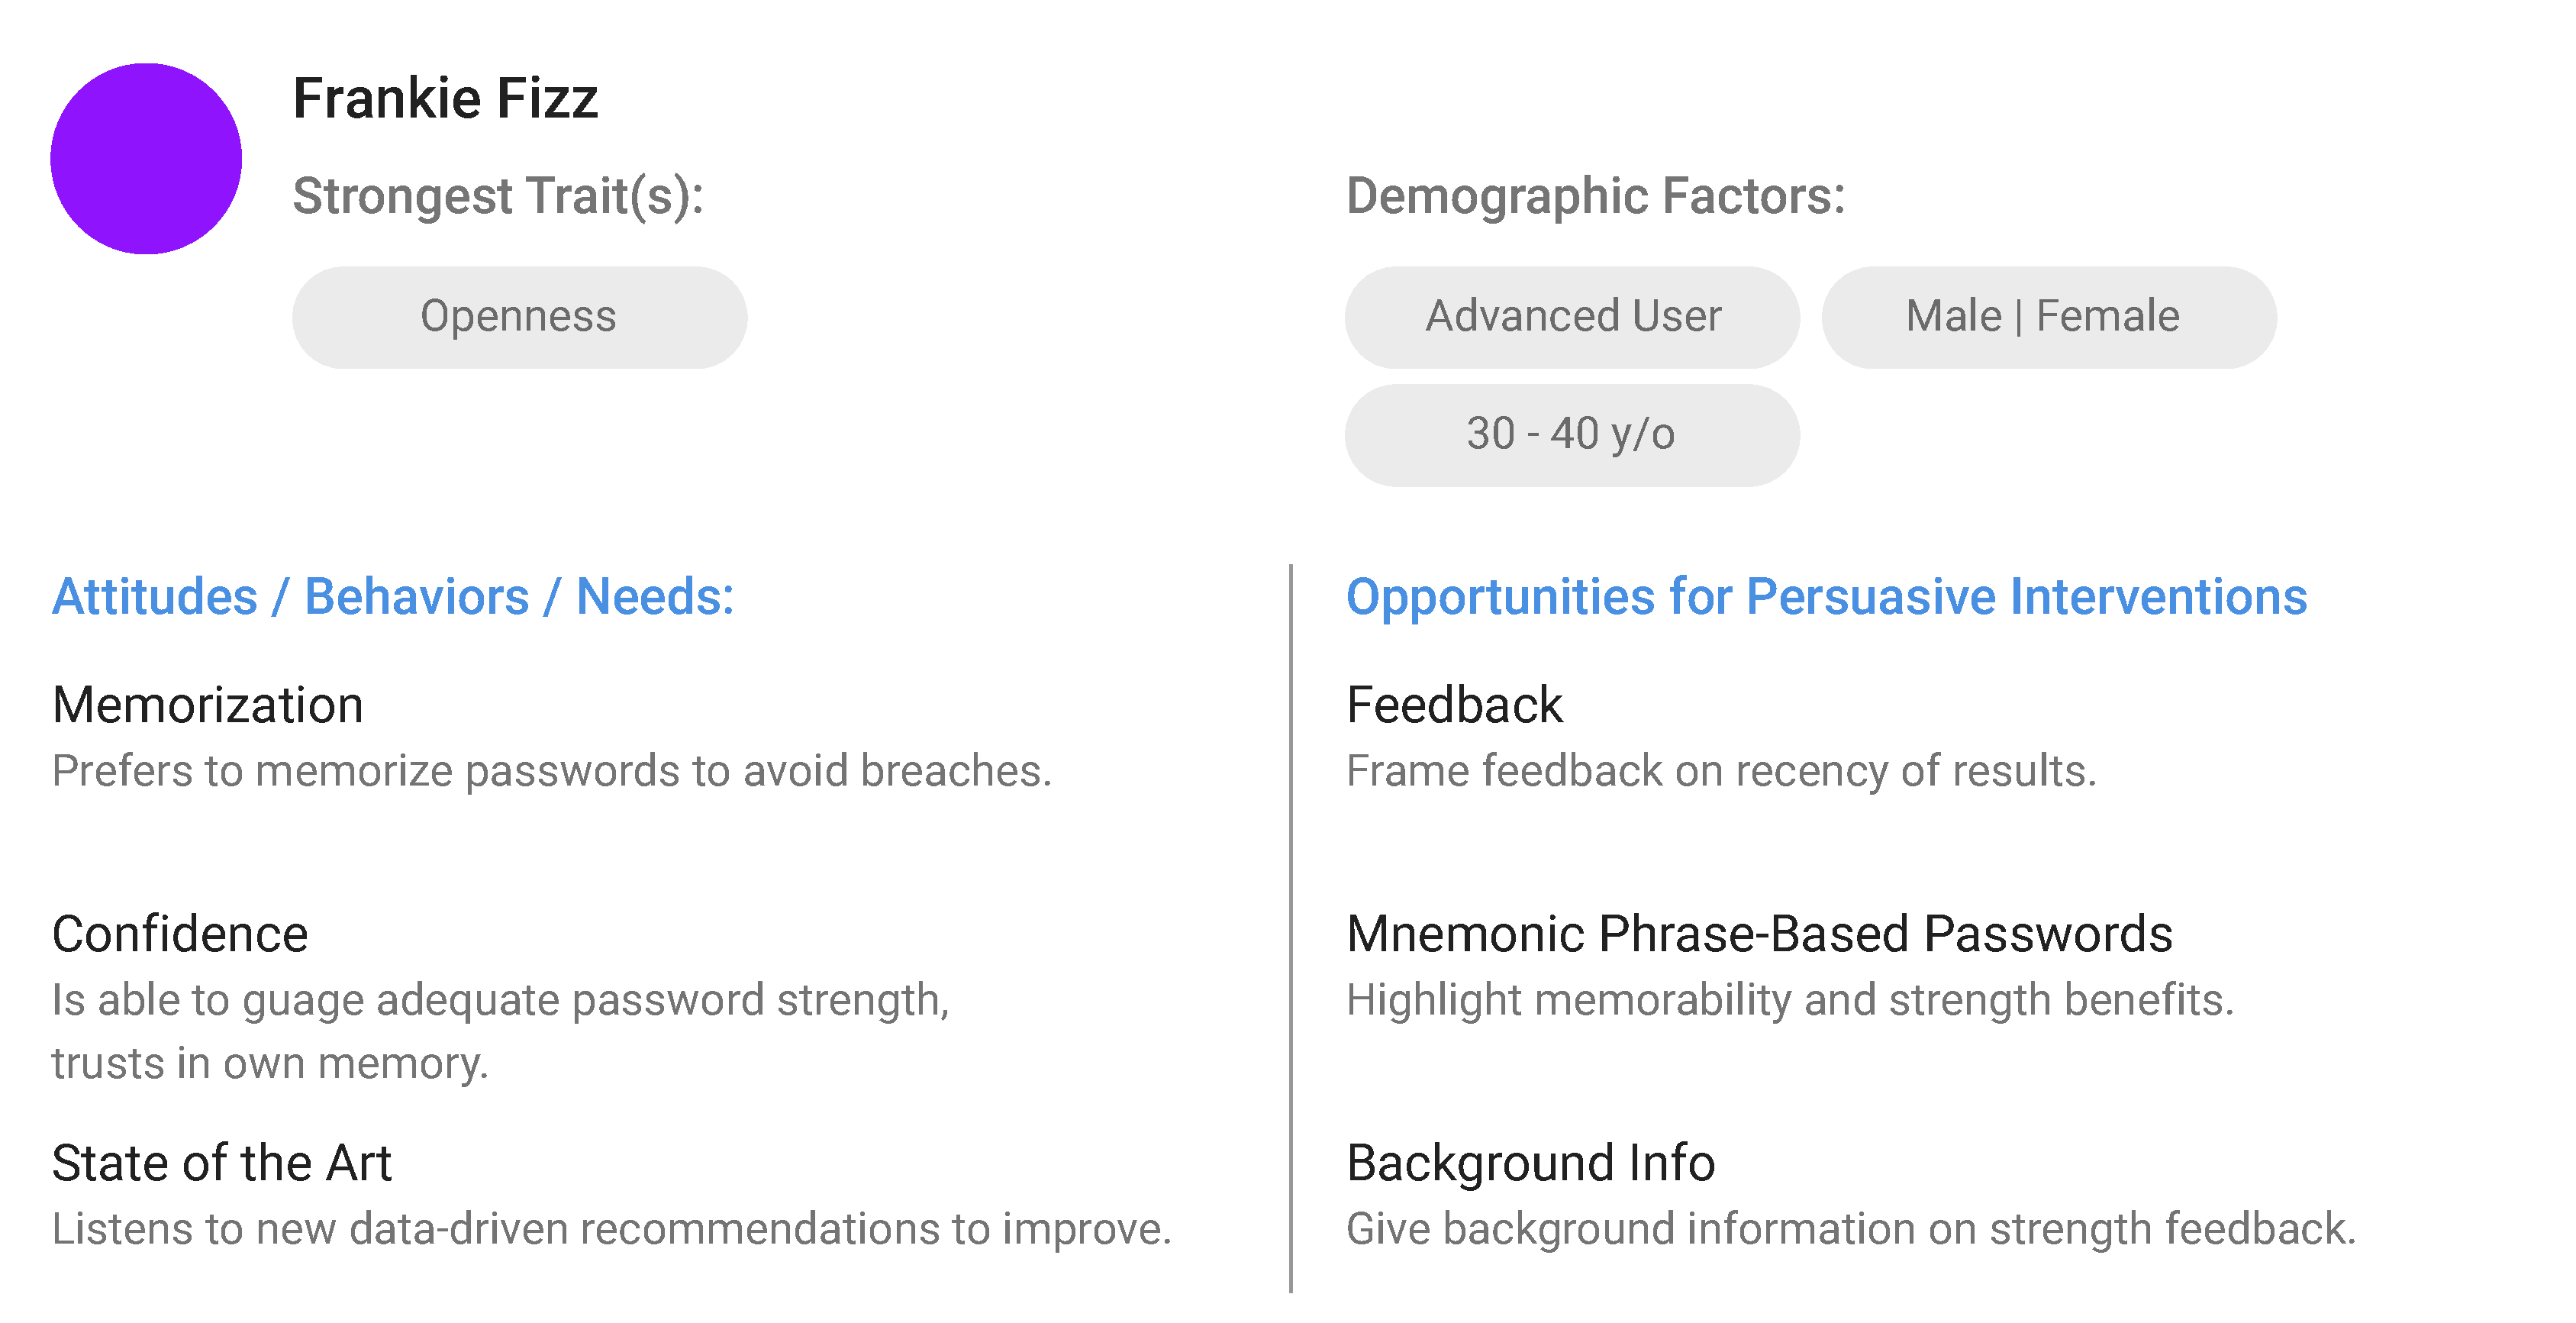
\includegraphics[width=0.7\linewidth]{personality/personas/Open-Persona}}
	\fcolorbox{dividergray}{white}{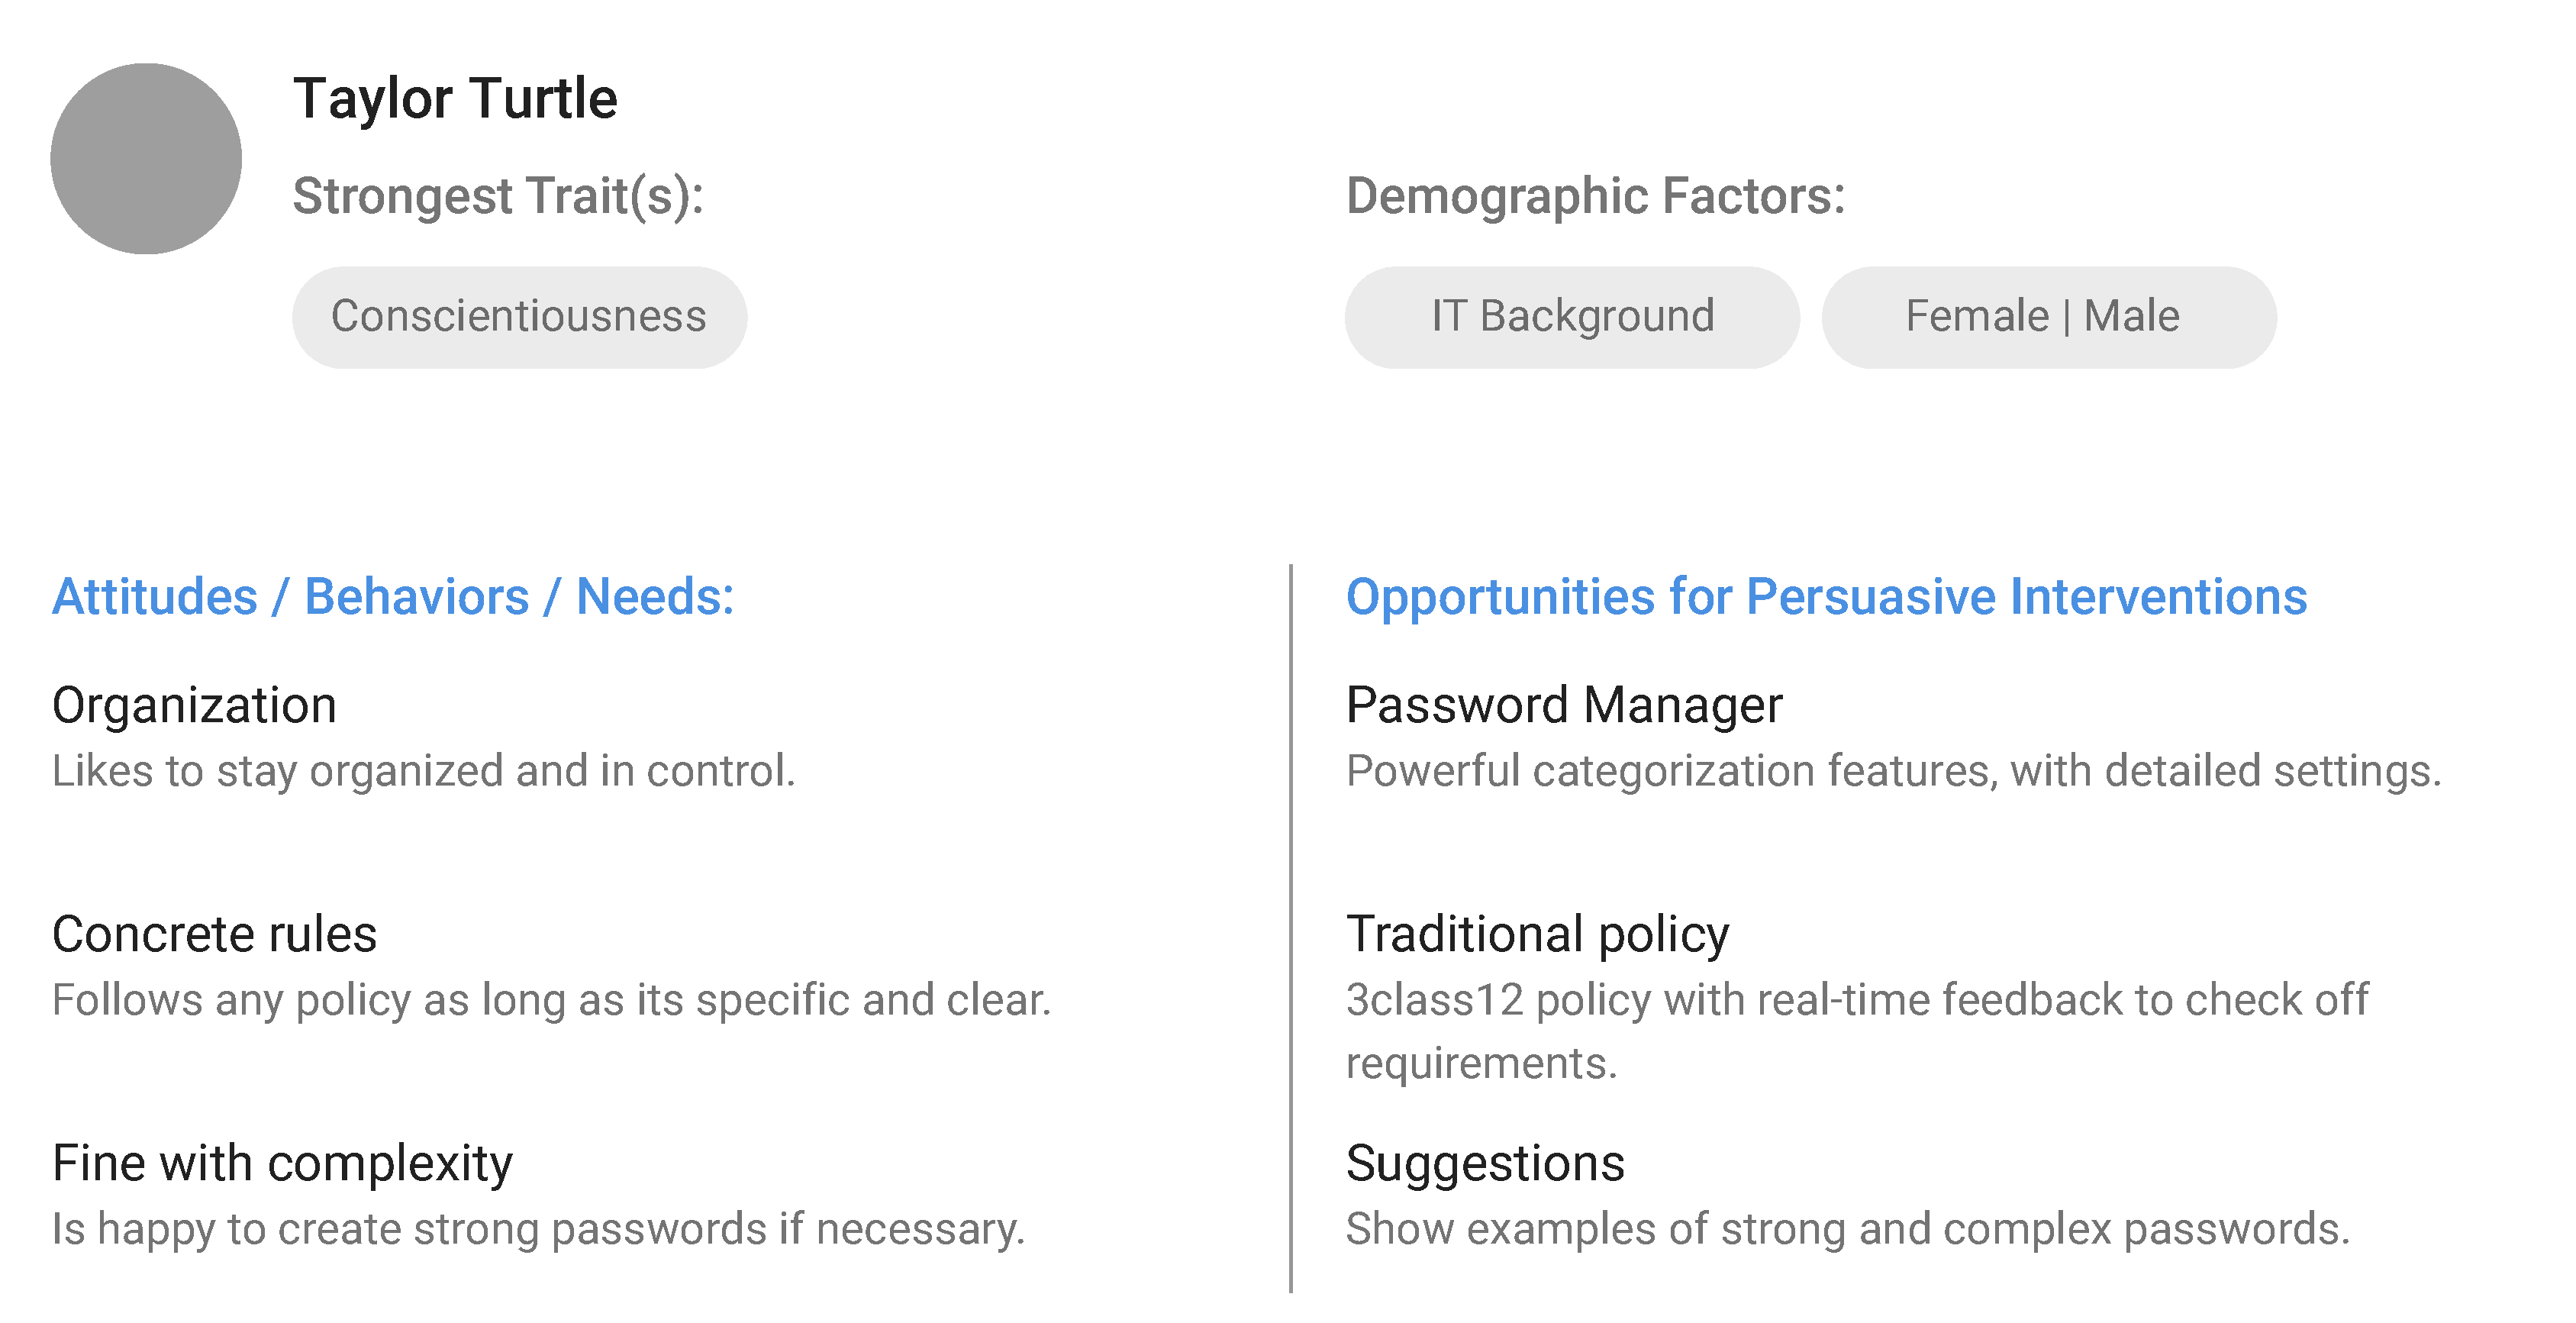
\includegraphics[width=0.7\linewidth]{personality/personas/Conscientious-Persona}}
	\fcolorbox{dividergray}{white}{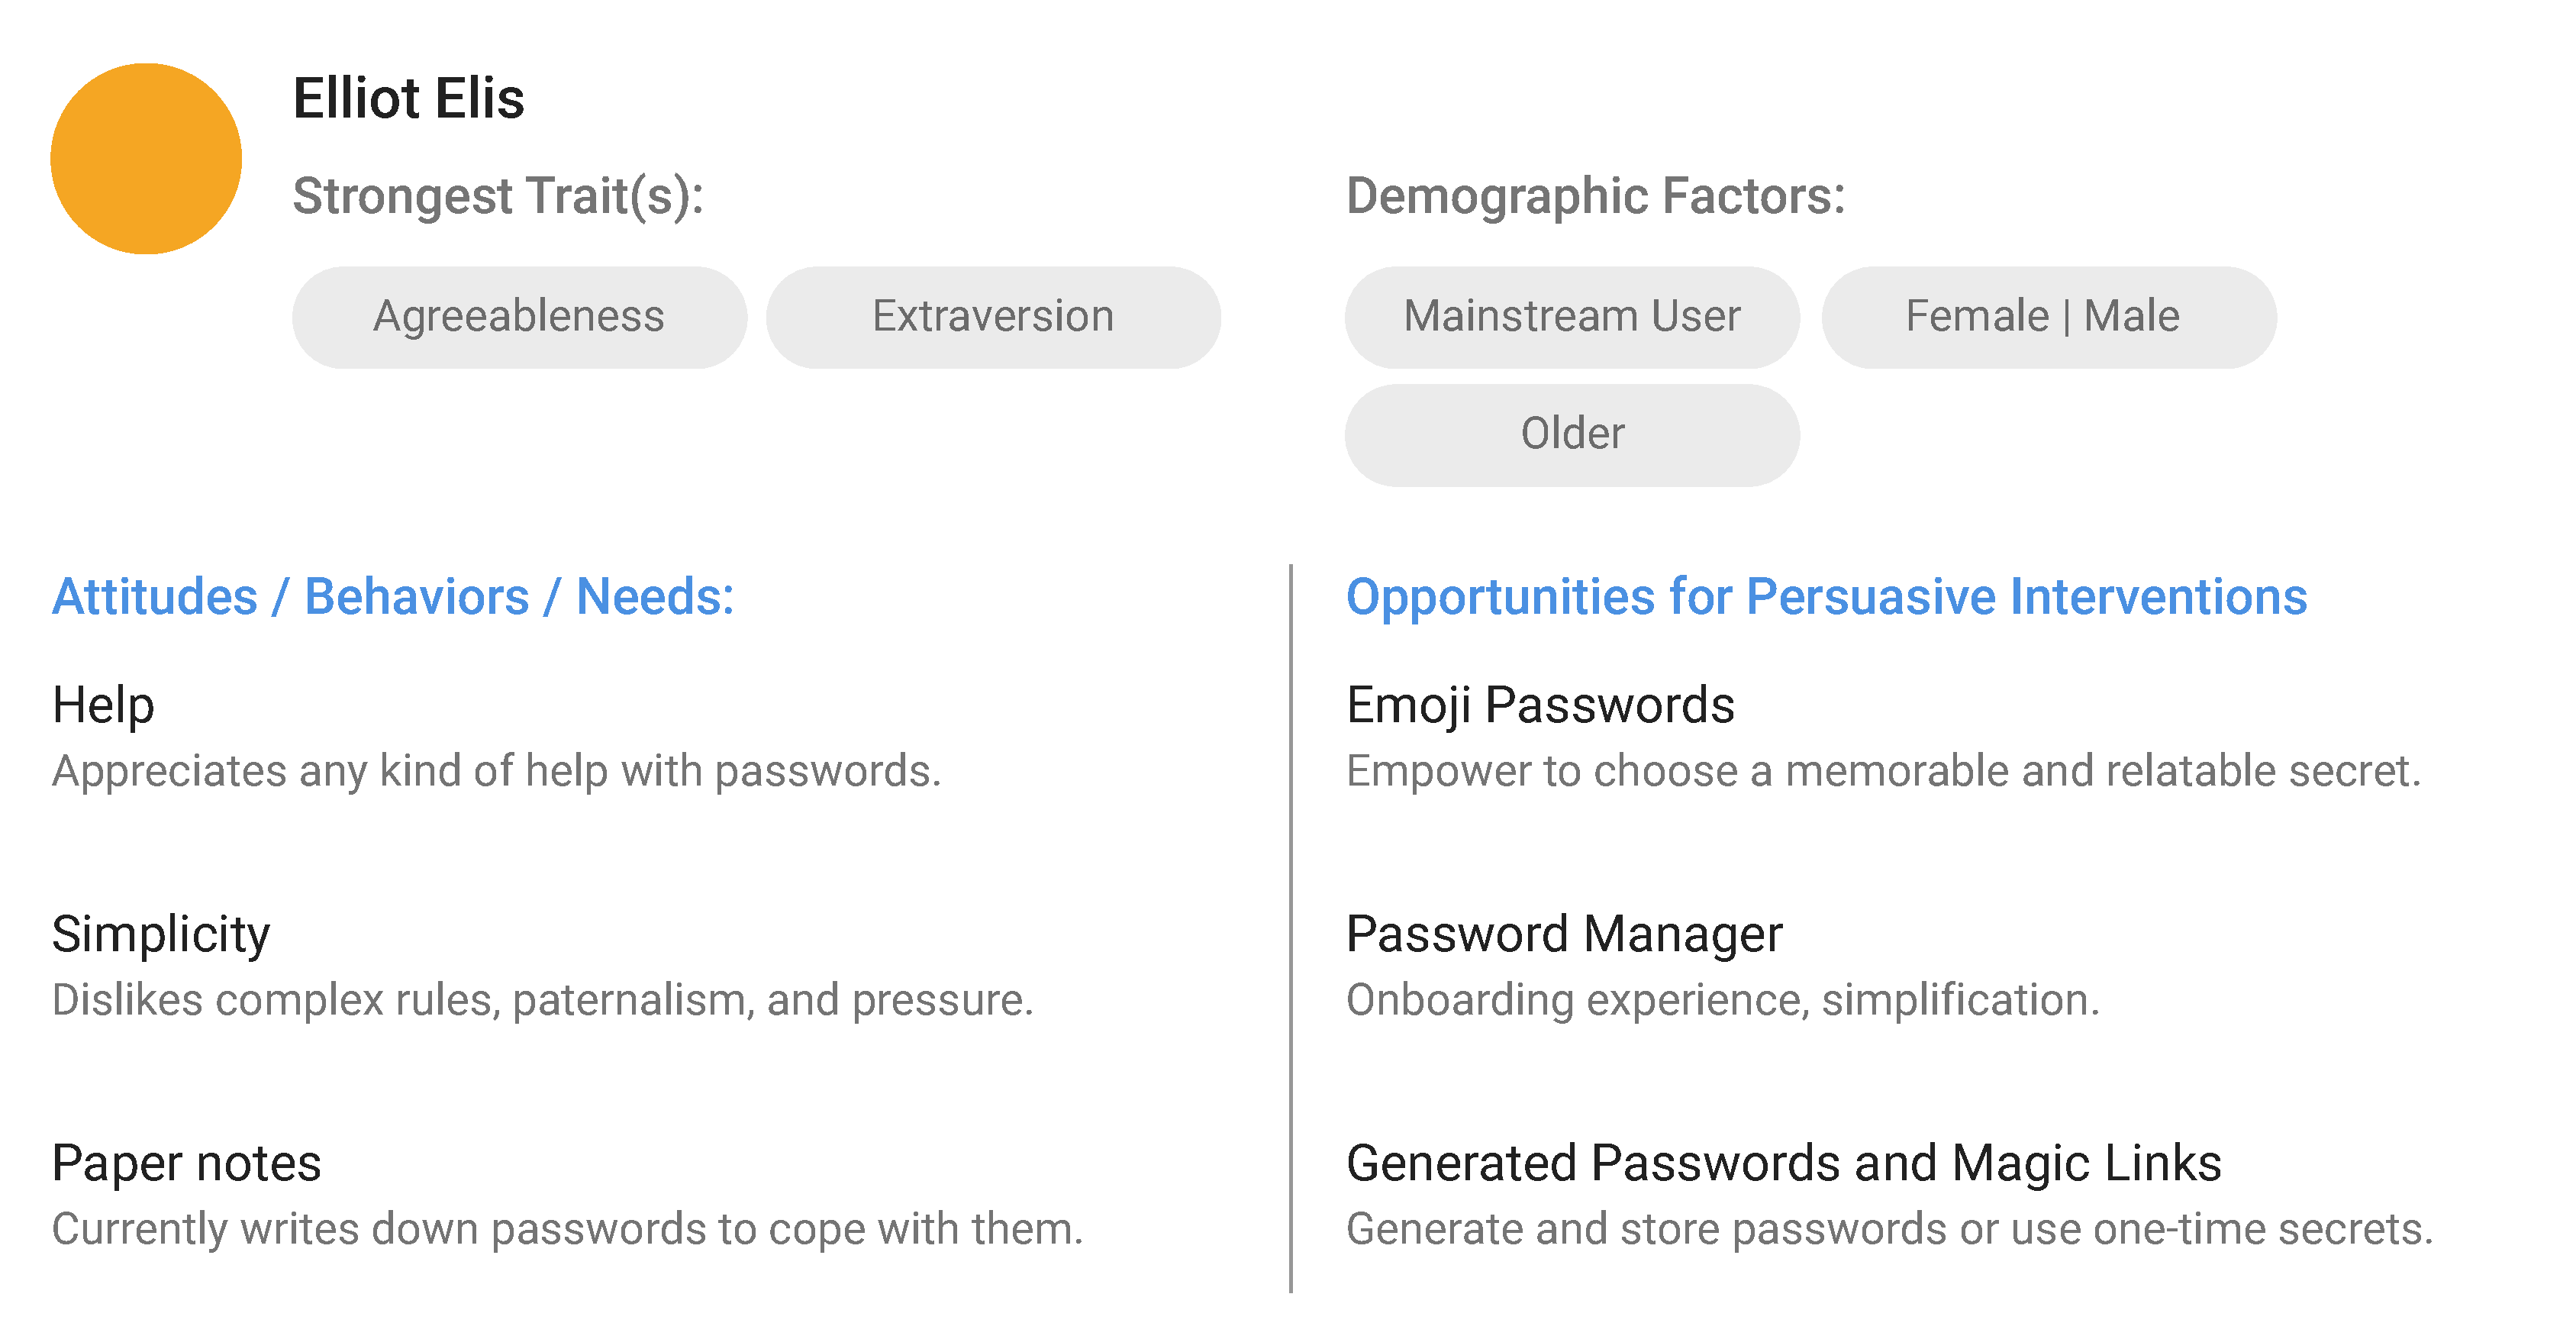
\includegraphics[width=0.7\linewidth]{personality/personas/Agreeable-Persona}}
	\caption{\label{fig:personality:personas} Password Personas. These fictional user profiles can inform design choices for password support strategies. Refining the details needs further research on password personality.}
\end{figure}

\subsection{Designing Feedback and Suggestions}
% strength suggestions
Using our personas, it is possible to address personality facets in real-time feedback during password creation. In the wild, we encounter password meters that estimate the strength of the password and in some cases even provide verbal feedback about what the user can do to improve the password (see  \cite{Carnavalet2014AnalyzingPWStrengthMeters,Wheeler2016zxcvbn}). A simple approach tries to convince the user to pick a stronger password by \textbf{suggesting a new one} or a modified version of the entered password \cite{Forget2008ImprovingPasswordsThroughPersuasion, Seitz2016SuggestionsDecoy, Shay2015SpoonfulOfSugar, Ur2017DataDrivenPWMeter}. 

Coming back to the finding that personality had a notable effect on how participants \textit{compared} two passwords, we suppose that it plays a role for real-time suggestions, too. How a modified version or newly generated password is received likely depends on the user's personality. On mobile devices, the user's password might be visible in clear text while they enter it \cite{Melicher2016UsabilityMobileTextPasswords}. Displaying an alternative password then resembles the comparison task from our study, and they might wonder which one is stronger. Strength feedback facilitates answering this question. It seems to be easier for \textit{conscientious} people to assess the strength of their password, if there is a clear list of requirements than can be ``checked off'', to make it superior to the suggested password (see the persona 3 ``Taylor Tang'' in Figure \ref{fig:personality:personas}). At the same time, users who strongly show the \textit{openness} trait seem to benefit from data-driven background information about the strength estimation algorithm. We conclude that Ur \etal's meter might be especially helpful for the persona 2 (Frankie Fizz). To make it work for persona 1 (Jamey Jones), it needs to be more reassuring than it currently is: The version presented at CHI 2017 constructively criticizes the user's password and suggests alterations. Adding a positive message might make persona 1 more receptive for this kind of suggestions. 

% coping suggestions.
Moreover, we found that demographic factors are useful to segment audiences. We found that older participants in our third study were more likely to appreciate if they do not need to memorize passwords, which was considered in persona 4 (Elliot Elis). They were more likely to use a password manager, paper notes or reusing passwords to reduce cognitive efforts. Thus, there is a great opportunity to suggest a coping strategy instead of a stronger password. For instance, websites or browsers could extend sign-up forms with a prompt to use a password manager. Pointing out the value of not having to memorize the newly created password could speak to older users and drive adoption rates. It is very important that the user journey from sign-up to password-manager set-up is simple enough to meet persona 4's needs. During account creation, interventions can leverage the ``opportune moment'': \textit{Kairos}, one of the persuasion principles presented in Section \ref{sec:rw:persuasive_patterns}, likely possesses a higher nudging power than, e.g. a news article recommending a password manager, because users are experiencing the problem first-hand during account creation. 

%\subsection{Tackling the ``Unknown User'' Problem}

%Results from the first study showed differences in the way participants dealt with password rules. The second study indicated that users the perception of password strength depends on both topology and personality. 

%Identity providers like Facebook or Google still rely on password authentication, and currently implement a ``one-fits-all'' policy. However, once users have used the services for a while, those parties already possess a large amount of user information. Consequently, the identity providers could alter the enforced policy for individual users depending on personality trait characteristics inferred from usage patterns. We propose to dynamically adjust the policy, for example when users reset their password. Users with an IT background could be asked to conform to a complex and long policy, while users showing stronger signs of neuroticism could be nudged towards including an emoji in their password. Such approaches could support the existing mental models of password strength and reduce user frustration with requirements. Ultimately, this can boost usability or user experience of the service. 
%TODO maybe inlcude the above part on emoji passwords / empowerment. 

% How can the segmentation be performed automatically without active user involvement?
% 	difficult questions -- smartphones
\subsection{Assessing Personality Traits in Password Studies}
In our studies, we \textit{explicitly} measured personality through psychometric constructs. This was straightforward, because online studies have become a reliable go-to method to study passwords. However, in many cases, omnibus tests like ANOVAs fail to reveal significant effects, and confounding variables could blur causality. Only few such covariates have been considered beyond demographic information. Our studies highlight that personality is a promising candidate to consider: for instance, average password strength perceptions were distributed normally. However, using general models, the underlying associations became visible and were statistically significant. Thus, psychometrics should not be neglected, so we can boost efficacy of security mitigations for different user segments \cite{Egelman2015AverageUser}. 

Still, extending surveys with long psychometric constructs is probably unrealistic. In our studies we used 50 and 21-item constructs. The latter already showed slightly reduced internal consistency. Thus, to keep studies short, to prevent participant fatigue, and to obtain reliable data, we propose focusing on the \textbf{openness} and \textbf{neuroticism} personality traits. Their associations were most stable in our studies and provided a coherent picture. They can be measured with only a couple of items (between 9 and 20), so the corresponding study part is finished within a few minutes. Nevertheless, the specific choice of the traits should be backed up by confirmatory studies in the future, and may also depend on the research question.

Adding even a few more items to a questionnaire might be impossible due to study constraints like budget or timeliness of data elicitation. There are, however, promising solutions to quickly and inexpensively obtain personality data on all dimensions from a user's past behavior. It is possible to infer personality facets from \textbf{social media data}, e.g. public interactions on Facebook \cite{Youyou2015Personality}. Youyou et al. found that such metrics can even outperform psychometric questionnaires. Stachl et al., as well as De Montjoye \etal found conclusive associations between \textbf{smartphone usage} and personality traits \cite{DeMontjoye2013, Stachl2017PersonalitySmartphones}. We thus suggest requesting permission to read either smartphone or social network data as part of the study. Crowd-workers in a large-scale study by Bentley and Chen, for instance, showed little concern to install software on smartphones for research purposes \cite{Bentley2015Phonebook}. While we would not go so far as to read all contacts, call and message history, we believe a differentially private\footurl{https://en.wikipedia.org/wiki/Differential_privacy}{04.03.2018} approach can replace personality constructs. 

% \todo{This argument is later revisited in the ``ideas'' an/or PST section, so maybe cross-reference it.}
 
\subsection{Statistical Models}
After consultation with statisticians, we opted for the use of generalized additive models (GAMs). Their usefulness hinges on the interpretability of their corresponding regression plots. Traditional indicators like (un-)standardized coefficients are limited in their contribution to gauge marginal associations and must be interpreted with special caution. In the case of logistic regression, standardizing binary variables is not useful, but we reported beta values to describe the slopes in the plots. Especially in study 2, we tried to select the model with the highest goodness of fit as indicated by the adjusted R-square value. We also considered the models' Akaike information criterion (AIC) to move forward. Here, increases and decreases of the AIC matched those of the R-square value. Interestingly, the models achieved better fit than related work on personality in privacy behavior \cite{Egelman2015AverageUser}. Thus, we advocate the use of GAMs in future analyses.  

\section{Conclusion and Future Work}
In three studies with a total of 440 participants, we broadly explored associations between personality traits and password behavior. This effort was one of the first of its kind. We focused on the relationship between the Big-Five model and password policies, strength perceptions, password selection, and coping strategies, while controlling for demographic factors. We found evidence for associations between (a) the usability of password policies and the neuroticism trait; (b) password strength perceptions and openness, respectively conscientiousness; (c) password length and neuroticism; (d) coping strategies and extraversion; and (e) IT-background and more secure behavior. Although the associations were not always particularly strong, they are still useful to inform the design of persuasive interventions and password policies. To that end, a set of four password personas was created to segment user groups by behavioral, attitudinal, and demographic archetypes. 

\subsubsection{Future Work}
Our work was of exploratory nature. Thus, the next step should be a focused study that increases statistical power to confirm or refute the associations. We provided a user segmentation in our personas to derive testable hypotheses. The refined knowledge about personality traits can be used to personalize password feedback and make it more effective. As pointed out by related work, some users overestimate the strength improvement of using digits in passwords \cite{Ur2016PerceptionsPassword}, which we also saw in studies 2 and 3. However, not all participants were equally influenced by digits or different character classes inside passwords. Respecting the psychographics in real-time feedback while carefully enforcing sensible policies could make these messages more effective. Besides, personality traits can inform choice architectures beyond passwords. For example, the Choose-Your-Own-Authentication approach \cite{Forget2015CYOA} can benefit from improved default settings depending on personality trait characteristics. The collection and aggregation of the necessary information could be done implicitly on mobile phones or social networks \cite{DeMontjoye2013, Stachl2017PersonalitySmartphones, Youyou2015Personality}. We see this a promising opportunity to improve the user experience of authentication mechanisms, because off-the-shelf technology can already achieve this goal. Finally, in light of some participants being more positive towards including emoji in their passwords opens new possibilities for password authentication. Emoji usage itself has been shown to be associated with personality \cite{Marengo2017EmojiPersonality}, which is supported by our research. Thus, it is important to investigate how personality traits might be exploited to model password strength of emoji-passwords. 

%TODO constellations like myers-briggs personality

\noindent
\fbox{
	\label{sec:personality:take-aways}
	\hspace{1cm}
	\parbox[c][15cm]{0.7\linewidth}{
		\section*{Take Aways}
		\begin{itemize}[leftmargin=*]
			\item Personality was weakly associated with all the measured dimensions: strength perception, policy preference / usability, password selection and coping strategies. Most notably openness, conscientiousness and neuroticism showed the most conclusive associations.
			\item The models for the perception of passphrases achieved the highest fit, suggesting a predictable association between personality and strength perception for this type of password. Comparing two passwords was associated with the conscientiousness traits. Mixed models that use both password features and personality trait scores as covariates were the most feasible approach to improve model fit.
			\item We can use ``Password personas'' to inform design decisions of persuasive interventions in the future. For instance, older users might be the best target group for password support tools, because age was a good predictor of their usage. Suggesting good tools during account creation might lead to higher adoption. Nudges designed for neuroticism should make emotional state more salient and positively reinforce the benefits of \underline{long} passwords. 
		\end{itemize}
	}
	\hspace{1cm}
}

 %published (short paper at Persuasive)
\chapter[Password Selection and the Decoy Effect]{Password Selection and the Decoy Effect}\label{chap:decoy}

% Motivation
% users use weak passwords a
% users think l33t speak is more secure than other strategies (pasdjo finding)
% but this is not necessarily the case, passphrases might be a better alternative
% hard challenge: mental model of passphrases indicates users think they are too weak. 
% RQ: how can this be changed?
% RQ: reverse misconceptions with ``marketing'' \cite{Ashenden2013SecurityLikeSoap}
% RQ: in which way do suggestions influence self-selected passwords?



%TODO Result summary. 
\section{Background and Context}

Goal: influence / correct mental models of password strength, persuade users to consider alternative strategies. 

Criticism: this is unrealistic because memory interference effects prevent that this works for more than one account. -- yes, but for important accounts, this might still be worthwhile and people can more easily write down three words instead of an 8 character random sequence that might include ambiguous characters (0 and O); Kuo et al also say that writing down is a perfectly valid strategy \cite{Kuo2006HumanSelectionMnemonic}. (\todo{look up more researchers who argue in favor of writign down, e.g \cite{Kothari2017PasswordLogbooks} })

\subsection{Suggestions}
Main topic: suggesting methods, feedback, modifications
\cite{Ur2012HelpingUsersCreateBetterPasswords}
\cite{Shay2012CorrectHorseBatteryStaple}
\cite{Shay2014CanLongPasswordsBeSecureAndUsable}
\cite{Forget2008ImprovingPasswordsThroughPersuasion}


\subsection{The Decoy Effect}
The decoy effect was discovered through research in consumer psychology. Buying a product usually involves deciding between different alternatives. On a high level, products are easily comparable by their quality and price, so customers heavily rely on these two metrics. The two dimensions also build the foundation of the decoy effect. In one of the first experiments on ``asymmetric dominance'', Huber \etal illustrate decision-making processes with a simple example to decide between six-packs of beer that differ in price and quality \cite{Huber1982AsymetricallyDominated} (slightly adapted for simplicity): 
\begin{table}[!h]
\begin{tabular}{lrr}
	\textbf{Option} & \textbf{Price} & \textbf{Quality rating}\\
	(A) & \$4 & 50 \small{/100}\\
	(B) & \$6 & 70 \small{/100}\\
\end{tabular}
\end{table}

While option (A) is cheaper than (B), it is also lower in quality. Spending \$2 more, the buyer will get a higher-quality beer (B). With the information available at this point, it is hard to decide. 
Buyers may have a general preference for either lower price, or higher quality if all other factors are excluded. Imagine the vendor wants to sell more of beer (A) because margins are higher for that product. To achieve this, Huber \etal explored different ways of adding a third option:
\begin{table}[!h]
\begin{tabular}{lrr}
	\textbf{Option} & \textbf{Price} & \textbf{Quality rating}\\
	(A) & \$4 & 50 \small{/100} \\
	(B) & \$6 & 70 \small{/100}\\
	(C) & \$4 & 40 \small{/100} \\
\end{tabular} 
\end{table}

Product (C) is as expensive as (A), but falls behind in quality. Thus, buyers will make a ``better deal'' if they choose option (A) by comparison with (C). Options (B) and (C) are more difficult to compare, because both dimensions (price and quality) are higher in (B) and make it appear like an outlier. Option (C) is thus called the \textbf{decoy} that is \textit{dominated} by option (A) (\textbf{target}). Option (B) (the \textbf{competitor}) also beats the decoy, but the comparability between the target and the decoy boosts the favorability of the target. This is exactly what Huber \etal found, and which was later confirmed numerous times in different decision-making scenarios \cite{Ariely1995ExplanationSubjectiveDominance}. Adding the decoy has the potential to reverse existing preferences, making it a powerful tool for marketing and sales. The decoy itself often serves the sole purpose of making another item stand out, thus the underlying persuasion principles are \textbf{salience} and \textbf{framing}. Constructing the dimensions in a certain way is referred to as \textit{choice architecture} \cite{Thaler2010ChoiceArchitecture}, and is an important persuasive design strategy. 

Huber \etal stated that there is a specific combination of attributes to position the decoy (see Figure \ref{fig:decoy:general-construction}). Depending on the target, the decoy acts as range increasing (R, R*), frequency increasing (F), or both (RF). By extending the range on the dimension on which the \textit{competitor} is superior, the fixed difference between all items on that dimension is weighed less. Figure \ref{fig:decoy:beer-construction} illustrates this type of decoy placement for the sixpack example. The range of the quality is clearer after the decoy is added: before the span was [50;70], and afterwards [40;70]. The superiority of the competitor appears less significant, hence the higher price can seem unjustified. 

%- decoy: vendor does not intend to sell this, it acts as an unfavorable alternative that can be used as reference point / comparison.\\	

\begin{figure}[t]
	\centering
	\begin{subfigure}[t]{0.49\textwidth}
		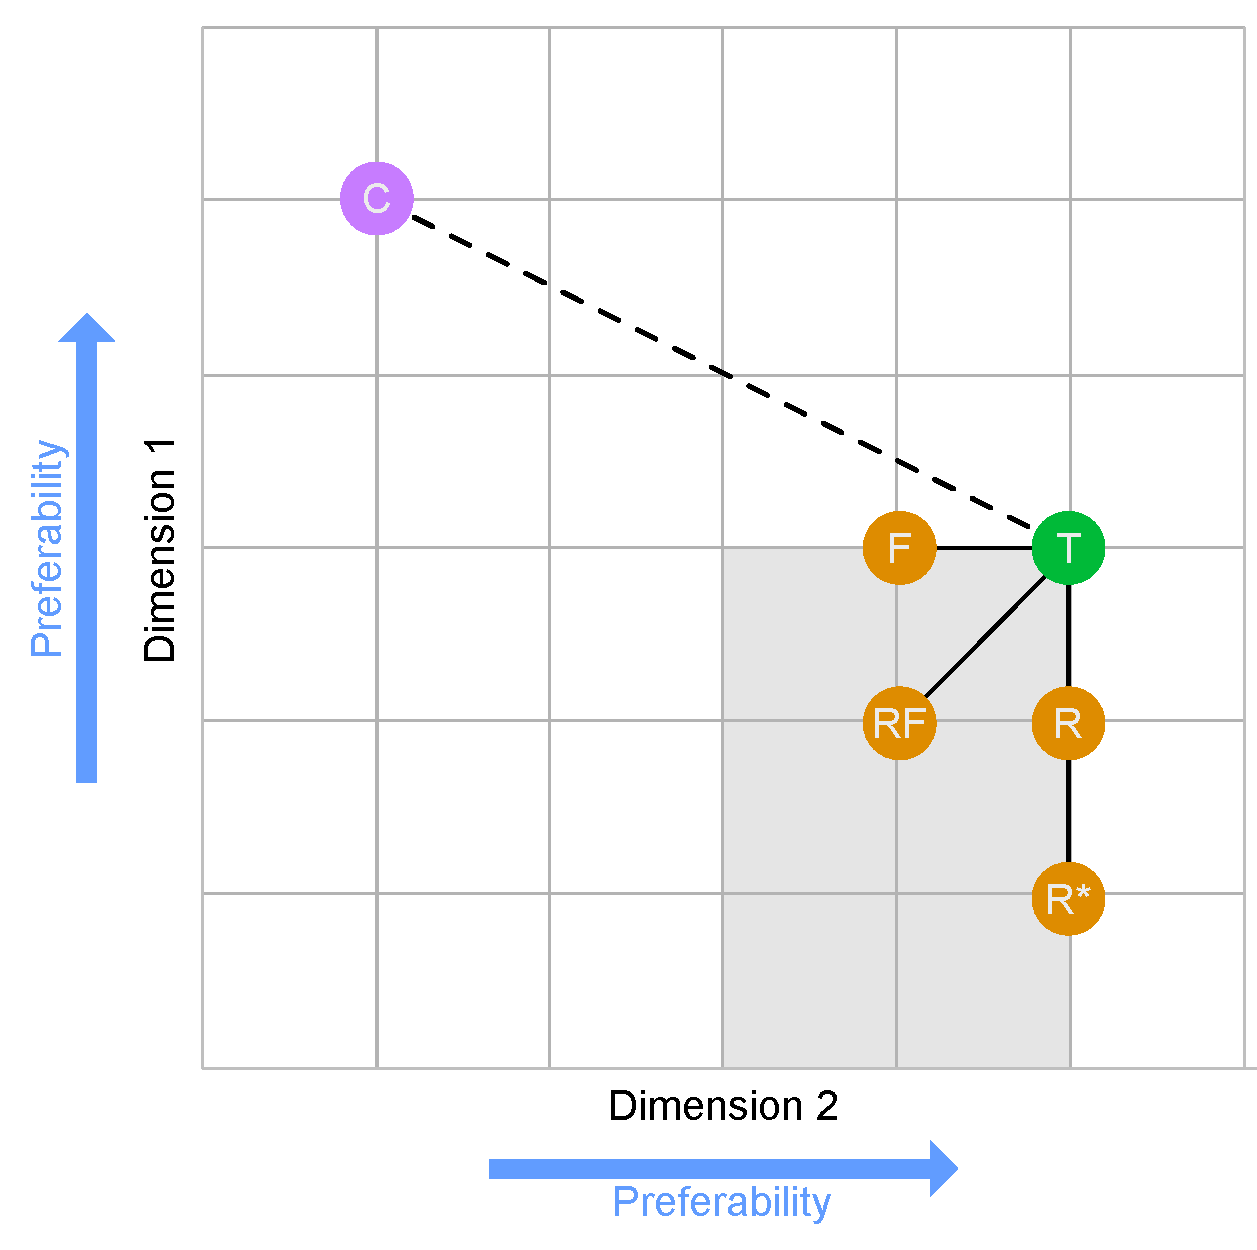
\includegraphics[width=\textwidth]{figures/decoy/decoy-dimensions-general}
		\caption{Decoy placement options \cite{Huber1982AsymetricallyDominated}}
		\label{fig:decoy:general-construction} 
	\end{subfigure}
	\begin{subfigure}[t]{0.49\textwidth}
		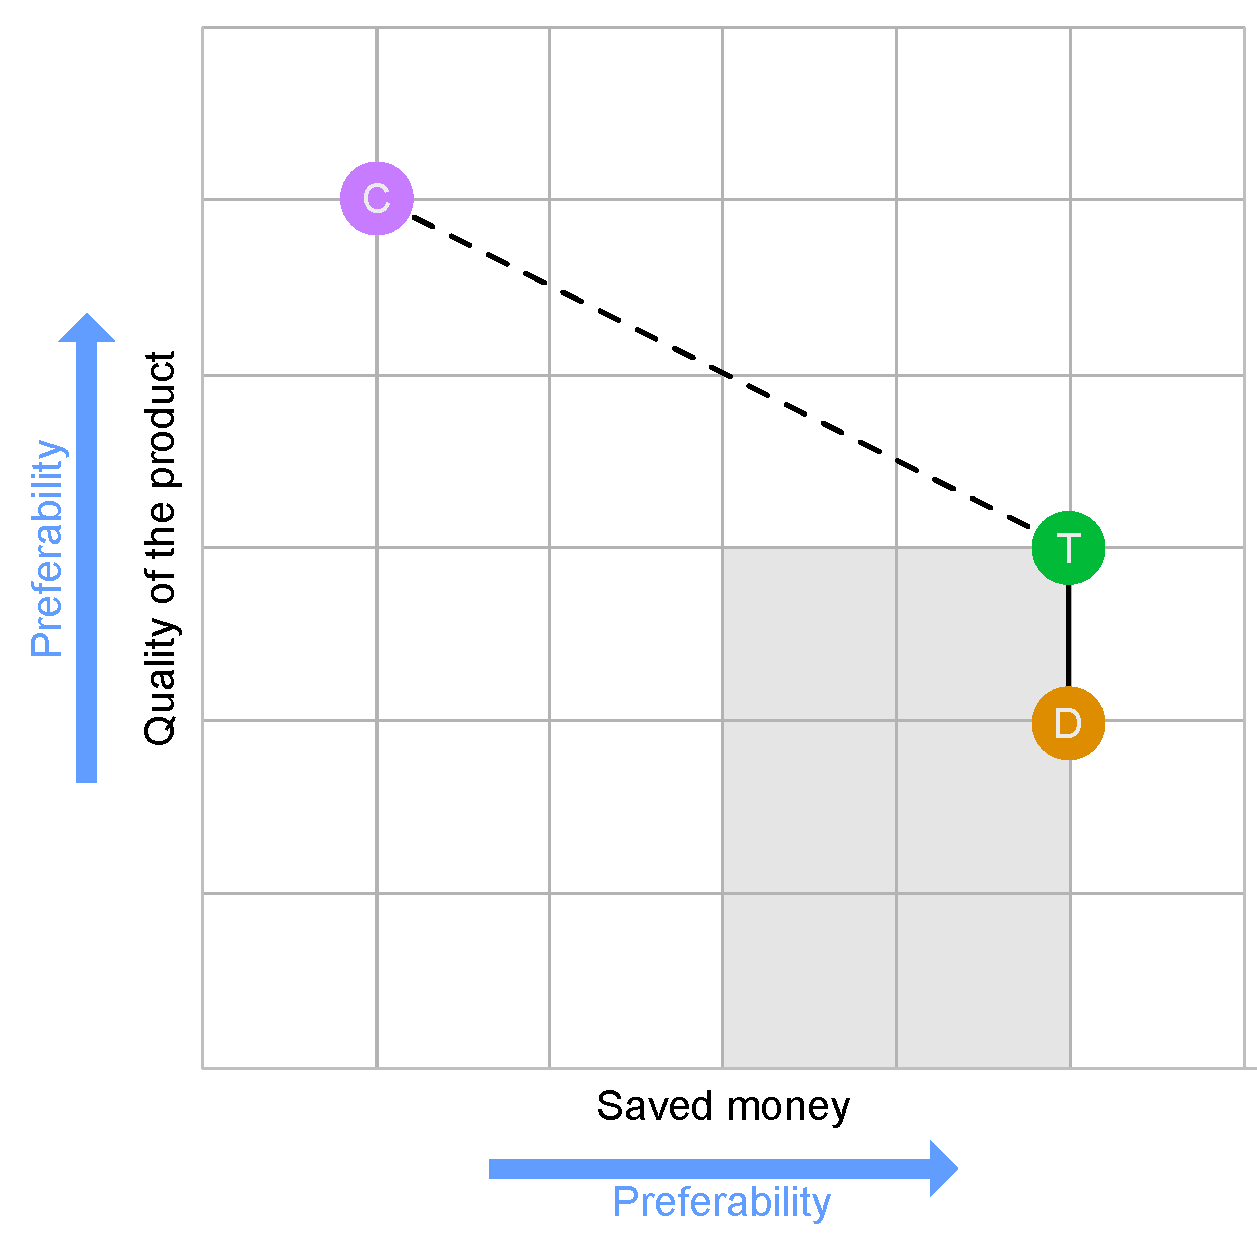
\includegraphics[width=\textwidth]{figures/decoy/decoy-dimensions-beer}
		\caption{Example choice architecture for sixpack of beers.}
		\label{fig:decoy:beer-construction} 
	\end{subfigure}
	\caption{
		General choice architecture overview to generate asymmetric dominance. 
		C = competitor, T = Target. The decoy can be placed at different positions in the spectrum, but needs to be dominated by the target (gray areay). Placement strategies for the decoy to increase the target's dominance: R = Range, R* = extreme range, F = frequency, RF = range and frequency.
	} 
\end{figure}

%- broader concept: framing, salience, anchoring. 
%- making choices, given a set of alternatives
%- using a decoy choice architecture to influence the preferred option 

\subsubsection{Example: Decoy Effects in the Real World}
Huber \etal's example has been adapted and used in the design of user interfaces. The vendor, i.e. a service provider, tries to steer users towards a particular direction that they see as favorable. For instance, location settings on an Android device show signs of a decoy pattern (see Figure \ref{fig:decoy:android-pattern}). From bottom to top, the ``device only'' mode activates the GPS module to determine the device's location. It is thus highly accurate outside of buildings, but does not work well inside. On the other hand, the ``battery saving mode'' works in both environments by using Google's online location services based on triangulation between network cells and surrounding WiFis. In urban areas and even inside buildings, it can achieve great accuracy, while it only roughly estimates locations in rural areas. The two accuracy-levels are thus comparable, but the ``battery saving mode'' does not require powering up additional antennae and modules, giving it a graspable advantage. The ``High accuracy'' mode combines both approaches and is thus the most battery consuming, but most versatile option. The ``battery saving'' can be seen as the target, because it provides the best trade-off in most situations. The ``device only'' mode is the decoy because it uses more battery, while the ``high accuracy'' mode is the competitor. Google requires the user to allow the collection of technical sensor data for the ``high accuracy'' and ``battery saving'' mode. Battery consumption is likely more important to users than location accuracy, which further suggests that the ``battery saving'' mode is indeed the targeted setting. 

\begin{figure}
	\centering
	\begin{subfigure}[!t]{0.49\textwidth}
		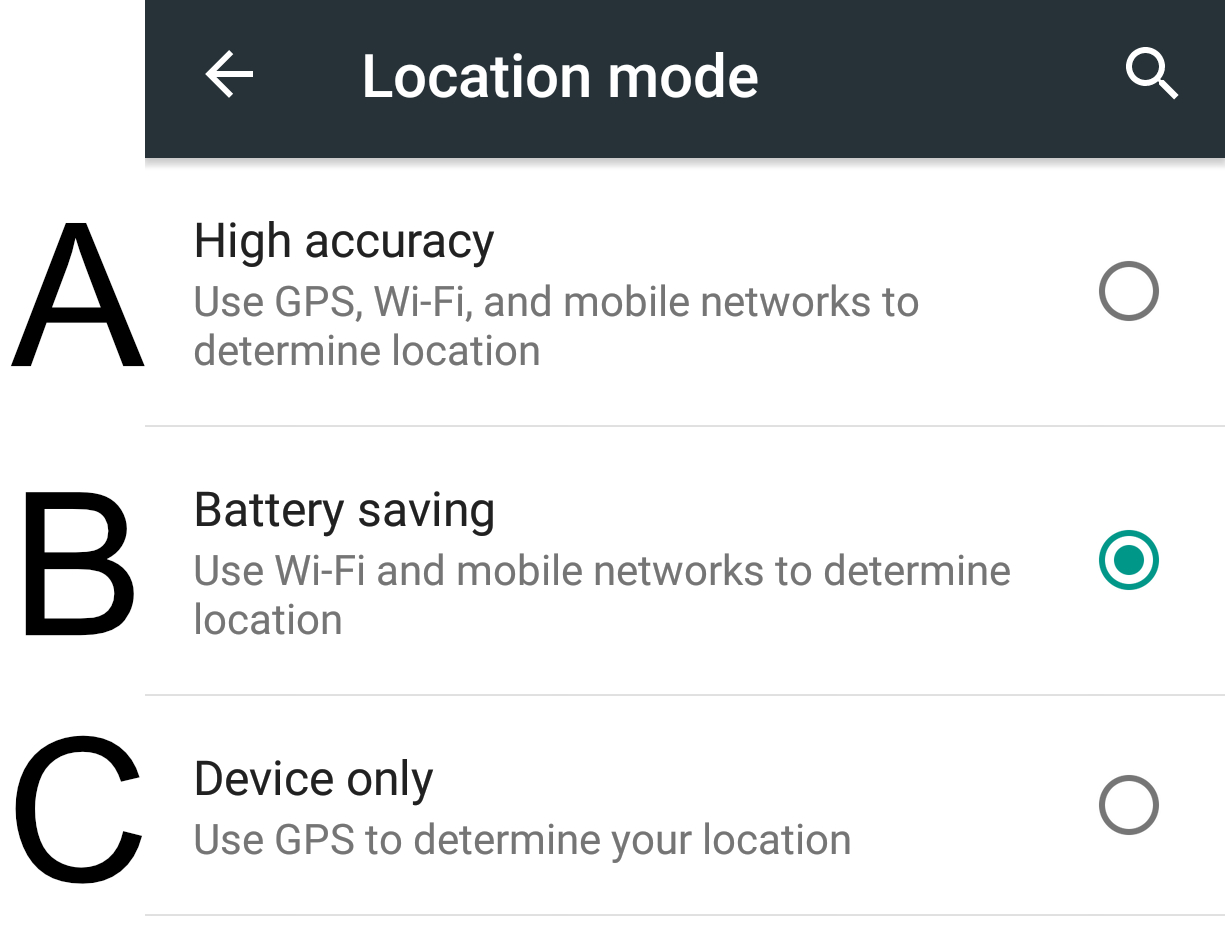
\includegraphics[width=\textwidth]{figures/decoy/Android_Location_Decoy}
	\end{subfigure}
	\begin{subfigure}[!t]{0.49\textwidth}
		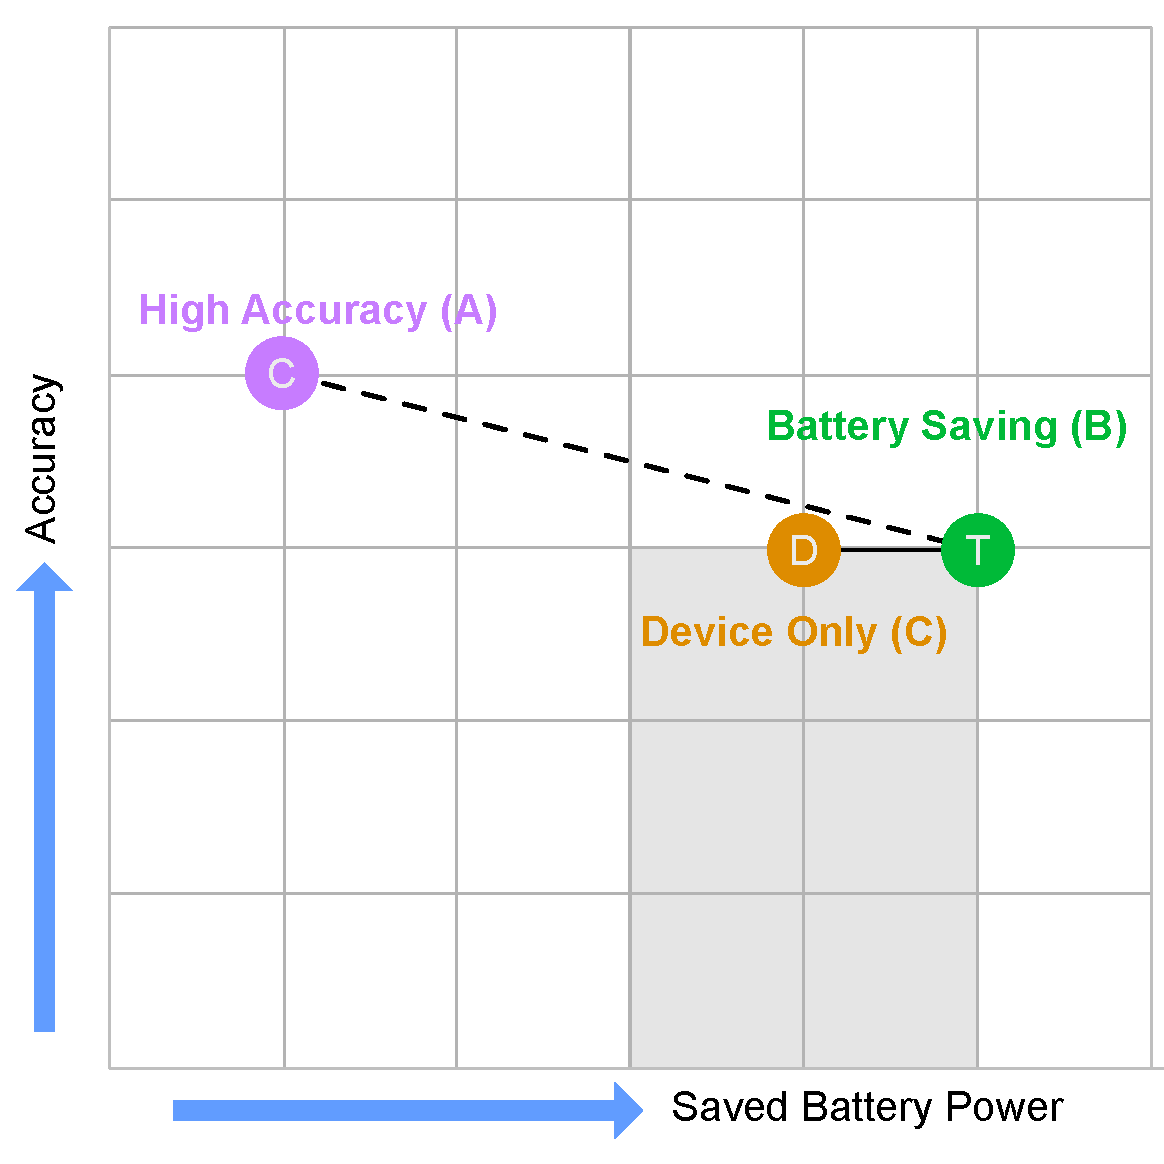
\includegraphics[width=\textwidth]{figures/decoy/decoy-dimensions-android}
	\end{subfigure}
	\caption{\label{fig:decoy:android-pattern}Location settings in Android show signs of a decoy pattern. The ``battery saving'' mode is targeted, because it does not activate the GPS module and can achieve comparable accuracy. Google benefits from collecting information on WiFi hotspots and network cells to improve their location service.} 
\end{figure}


\subsection{Choice Architecture in Security and Privacy}
The \gls{USEC} community has started to investigate the feasibility of behavioral economics principles in the design of security and privacy mitigations. Egelman \etal showed that choice architecture is highly relevant for privacy settings on mobile devices \cite{Egelman2013ChoiceArchitecture}. They explored how users value privacy-respecting apps and how they make decisions from a list of applications. To measure preferences, they put monetary values and discounts on permissions like accessing the Internet or using device location. Participants in their study showed clear decision-making patterns that were influenced by the price and type of permission. Therefore, Egelman \etal concluded that a certain choice architecture can guide users towards a more ``rational behavior''. 

Knijnenburg \etal \cite{Knijnenburg2013MorePrivacyOptions} explored the \textit{choice proliferation} phenomenon in location-privacy settings. The principle indicates that people become choice averse with an increasing number of options. In their study, they observed that participants were strongly influenced by the number of available options to share their location. Without specifically mentioning it, they also used a \textit{decoy} option that was extremely unfavorable, but triggered a change in preference. In another study, Korff and Böhme showed that the granularity of privacy settings on a business social network can have similar effects: participants in their study tended to stick with default settings and were also less satisfied with their choices \cite{Korff2014TooMuchChoice}. Acquisiti \etal showed that such architectures can nudge users towards certain settings \cite{Acquisti2017NudgesPrivacySecurity}. 

Regarding passwords, only few publications mention the use of choice architectures. Renaud \etal evaluated a wide range of nudges to make users of a university platform pick a stronger passwords. They concluded that the tested architectures were fairly ineffective in achieving this goal, but there might have been other more effective solutions beyond their designs. Before our own investigation, no study that we are aware of has explored the decoy paradigm for passwords. 

% might be mentioned briefly:%
%\cite{Wang2014PrivacyNudgesFacebook}
%\cite{Malkin2017PersoanlizedSecurityMessaging}
%\cite{Jameson2011PreferentialChoice}

\section{Designing Password Choice Architecture}
% Briefly point to first exploration report to mention a design that failed. 
We aimed to craft a nudge that persuades users to create stronger passwords. Respecting the principle of the opportune moment, we opted for account creation contexts. To emulate a situation that is comparable to buying one out of several product alternatives, we show suggestions beneath the password field where the user enters their choice (see Figure \ref{fig:decoy:design-architecture-prolific}). We ended up with this design after identifying opportunities of strength feedback on the user's password and on the suggestions (i.e. feed-forward). To that end, we had created several prototypical choice architectures and rapidly evaluated them in the lab and online (see technical report \cite{Seitz2016DecoyEffectReport}). The final architecture implements the propositions in Huber \etal's framework (see Figure \ref{fig:decoy:dimensions-prolific}).

\begin{figure}[t]
	\centering
	\begin{subfigure}[!t]{0.49\textwidth}
		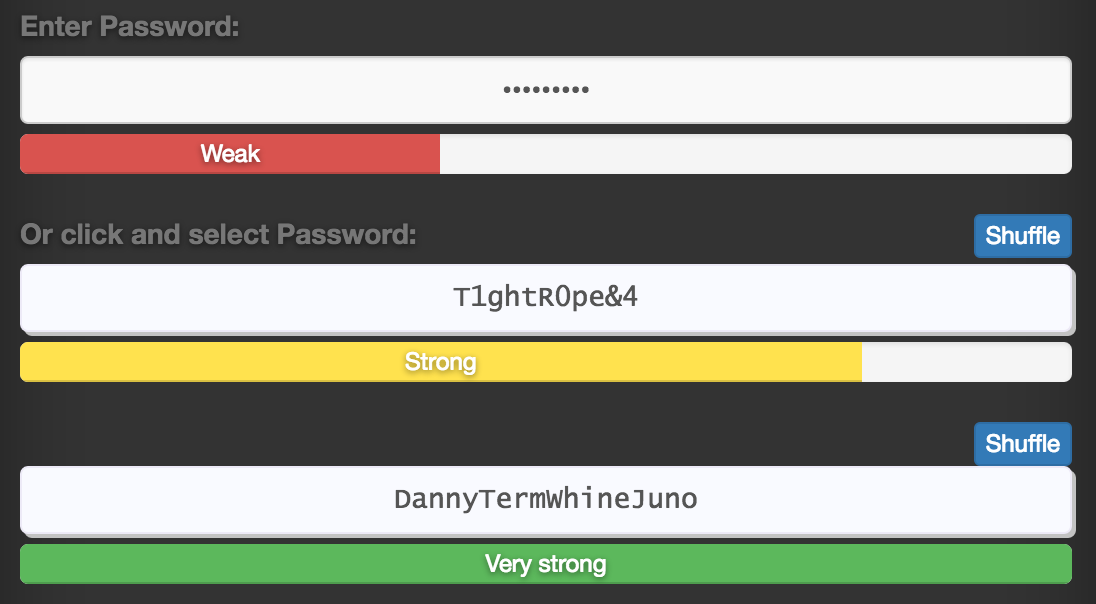
\includegraphics[width=\textwidth]{figures/decoy/generator_prolific_3}
		\caption{\label{fig:decoy:screenshot-prolific}}
	\end{subfigure}
	\begin{subfigure}[!t]{0.49\textwidth}
		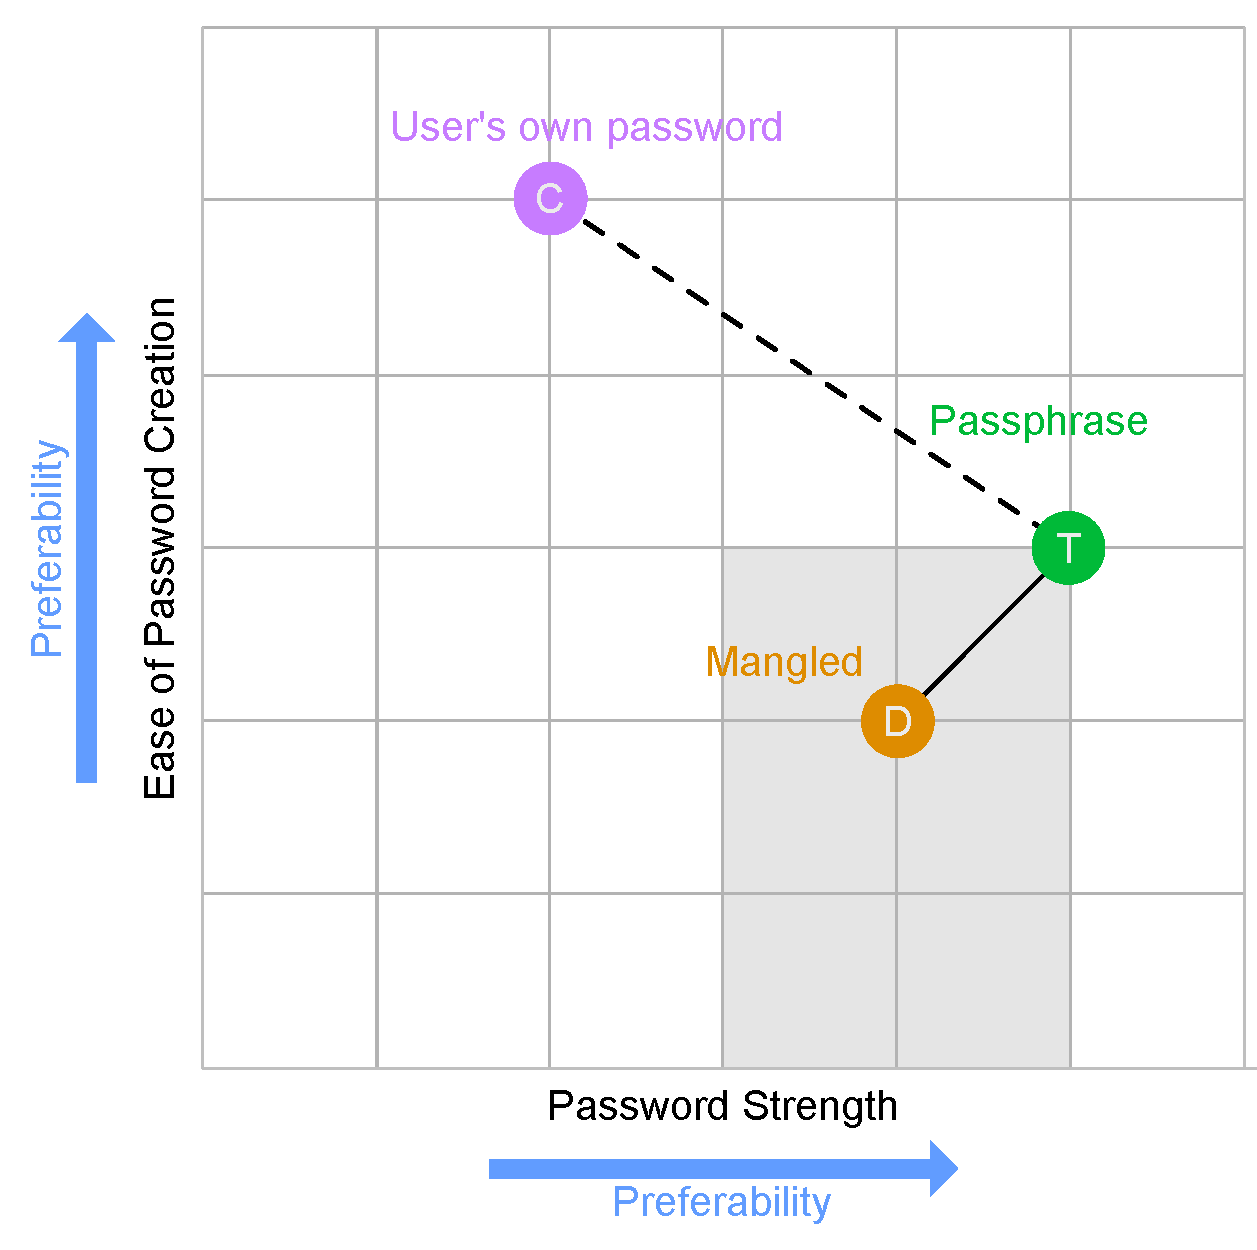
\includegraphics[width=\textwidth]{figures/decoy/decoy-dimensions-prolific}
		\caption{\label{fig:decoy:dimensions-prolific}}
	\end{subfigure}
	\caption{\label{fig:decoy:design-architecture-prolific}Choice architecture and decoy placement as evaluated in the online experiment. } 
\end{figure}

The key to password choice architecture is the user's own password. It has to be seen as the \textbf{competitor}. Service providers will want accept the user's own password, because they want make sure users sign up. On the other hand, they want to avoid attacks on user accounts, which is why they likely encourage using a stronger password. This is the \textbf{target}. In our design, we opted for a \textit{passphrase} as target for several reasons: only few users create secure passphrases as their primary credentials \cite{Ur2015PWCreationLab}; passphrases provide usability and memorability benefits \cite{Keith2009PassphraseDesign}; self-selected passphrases often do not provide the desired security benefits \cite{Bonneau2012LinguisticProperties}, which can be mitigated by supplying users with a combination of random words \cite{Shay2012CorrectHorseBatteryStaple}. 

To make the passphrase preferable over the competitor, a decoy needs to be carefully positioned along the two dimensions such that it is closer to the target than to the competitor. Moreover, it needs to be dominated at least in one dimension by the target. To achieve this, we identified ``ease of use'' and ``security benefits'' as two feasible dimensions of the choice architecture. We opted for a range-frequency decoy (see Figure \ref{fig:decoy:general-construction}) where the target dominates the decoy in \textit{both} dimensions, because effects are more likely to be detected this way. A typical-length \textit{mangled} password fulfills the criteria. The richer character set includes symbols that require the Shift/Alt keys to enter them. Thus, the ease of creation is lower than that of a passphrase (dimension 1). At the same time, typical mangling strategies only slightly contribute to password strength, which we confirmed in Chapter \cite{chap:pasdjo}. Passphrases are considered stronger by several estimators. Consequently, mangled passwords are dominated by passphrases regarding strength (dimension 2). Figure \ref{fig:decoy:dimensions-prolific} illustrates the positioning along the two dimensions.

\section{Quantitative Evaluation}
We ran an online experiment to evaluate the efficacy of our decoy choice architecture for passwords. We formed the following hypotheses about the outcome:
\begin{description}
	\item[H0] Participants' self-selected passwords are comparable in strength and memorability, regardless of the presence of a password suggestion (Nullhypothesis). 
	\item[H1] The presence of a single password suggestion will lead to slightly stronger passwords.
	\item[H2] The presence of two suggested passwords that follow a decoy choice architecture regarding strength and ease of use will lead to stronger passwords that resemble the target suggestion. 
\end{description}

\subsection{Method}
% study design, independent variable
The study implemented a between groups design. The main task was creating a new password under one of four treatments. ``Suggestion architecture'' served as independent variable with three levels: \textbf{Passphrase}, \textbf{Mangled}, and \textbf{Decoy}. Each level was tested with a separate participant group. In the Passphrase condition, participants were suggested a single passphrase consisting of four words. Analogously, a higher-complexity password is displayed in the Mangled condition. The Decoy group received both the target passphrase and the complex decoy password as alternative suggestions to their own password. Having study conditions with single suggestions allowed us to measure the impact of the decoy effect. All suggestions are accompanied by visual and textual representations of zxcvbn scores. The labels for the different strength scores were \textit{very weak, weak, ok, strong, very strong}. To obtain a baseline for comparison, there were no password suggestions for the \textbf{Control} group. However, participants in this group received strength feedback allowing us investigate the impact of suggestions. 

%dependent variables
We did not collect plain text passwords to ethically deal with participants disclosing their real passwords. Instead, we used modified the zxcvbn library by stripping all sensitive information\footurl{https://gist.github.com/TobiasSeitz/e27a867535b82f6cf9a6ae6140da8b81}{06.03.2018}, and analyzed participants' passwords on the fly. These \textit{meta statistics} served as dependent variables and were saved to a regular database. Most notably, they describe the password topology (length, number of upper-/lowercase, digits, symbols, and chunks), estimated guess numbers and the zxcvbn score. Scores range from 0 (weak) to 4 (strong), while guess number estimates are open-end. Another dependent variable was memorability which was measured by a successful authentication three days after password selection. To achieve this, we hashed passwords with a secure one-way function (PHP's \texttt{password\_hash()}) and compared hashes afterwards. If they matched, the password was correct, thus this is a binary metric.

\subsubsection{Prototype}
For the purpose of the study, we implemented the concept as web-prototype based on HTML and JavaScript. As foundation for the generating passwords in all conditions, we relied on the Diceware dictionary\footurl{http://world.std.com/\~reinhold/diceware.wordlist.asc}{06.03.2018} consisting of 5823 words. It provides a good spectrum of common and uncommon words of varying length. To generate the passphrase (target), four words were randomly combined and capitalized individual words. As shown in Chapter \ref{chap:pasdjo} zxcbvn rates four-word passwords with its highest score. The randomness of generated passwords allows us to calculate their entropy. Each word has an estimated entropy of $(log_2(5823) \approx 12$ bits. Combining four words randomly thus results in a total entropy of approximately $ (2^{12})^4 = 48$ bits for passphrases.

For the decoy and the mangled password condition, the prototype modifies a randomly selected word from a smaller subset of the Diceware list. The subset only includes words longer than eight characters, giving a total of 687 candidates. The first letter of the word, and a second randomly chosen character are capitalized. Two letters are substituted by similarly-looking digits to inspire a \textit{l33t} character. For instance, the letter ``o'' was replaced with the digit ``0''. Finally, a random symbol and digit are appended to the word. The resulting decoy password consists of four different character classes (LUDS). 

We anticipated that the generated passwords are exceptionally unattractive in some cases, e.g. if passphrases consist include uncommon, hardly memorable words, e.g. \texttt{GirthInflixThineAegis}. To make them more appealing, the prototype provides a \textit{shuffle} button that gives a new combination of words (see Figure \ref{fig:decoy:screenshot-prolific}). The mangled password can also be re-generated. Another feature to lower barriers to take one of the suggested passwords was the opportunity to transfer it to the password field with a single click. However, to facilitate memorization, participants needed to manually type the password into the confirmation field. 

\subsubsection{Procedure}
The experiment consisted of two parts that were carried out on separate days. The initial step included the password selection task and usability assessment among other qualitative metrics. Participants were invited to return for the second part of the study three days later. This follow-up step included memorability assessment and further qualitative feedback to help us understand the data.

The first part started with a thorough briefing about the collected data and asked for consent. The same web-page introduced the scenario for the task: Participants were asked to imagine creating a new password for their already existing email account under a basic8 policy. The page displayed the password fields and suggestions. Participants were randomly assigned to one of the four treatment groups, so the type and number of suggestions depended on this assignment. Once the password was successfully confirmed, participants were asked to fill out a brief questionnaire mostly consisting of 5-point scale items on attitudes and password behaviors. At the end of the first part, the web-page displayed a confirmation code that participants had to copy over to the prolific platform to mark the survey as done. 

Three days afterwards, we invited the participants to return and complete the second part. They were asked to provide the password they had remembered, but we did not validate 

\subsubsection{Recruitment and Sample}
Following best practices in password research, we leveraged crowd-sourcing tools to elicit the data. Recruitment took place through the research platform Prolific\footurl{https://prolific.ac}{06.03.2018}, which is comparable to Amazon's Mechanical Turk solution. Participants were screened for age (older than 18 years), and they had to be located in either the UK or in USA. The region restriction was introduced because Prolific has a larger user base in those countries. To ensure quality of the data, we required a past survey completion rate of at least 95\%. This is a common metric for the reliability of a crowd-worker \cite{Ross2010WhoAreTurkers}. 

From the 106 respondents who started the experiment, we had to reject seven because the study completion code was wrong or missing, or because the questionnaire was insufficiently filled out or completion times were outliers ($> 3*SD$). The remaining 99 participants received invitations to return, which 97 people did. There were another fourteen incomplete responses or wrong study codes. Hence, the resulting N of our data set is $N = 83$ valid, complete responses in both parts. Group sizes were $n=18$ in Control, $n=24$ in Passphrase, $n=21$ in Mangled, and $n=20$ in Decoy. On average, participants were 30 years old ($SD=10$). 42\% were female. The majority (78\%) was employed, 12\% were students, 10\% were unemployed. Participants reportedly possessed nine online accounts that they regularly use ($SD=5.6$). 

%no CS students: just like in \cite{Wash2016UnderstandingPasswordChoices}

%live deployment. 
%users could shuffle. 

\subsection{Results}
Through statistical tests we found significant differences across the groups. Although the decoy effect did not work as intended, there were notable side-effects. In the following, we break down the findings. For non-parametric continuous data, we used Kruskal-Wallis and Mann-Whitney tests, whereas frequencies were analyzed with chi-squared tests. Significance levels were set to $\alpha = 0.05$, unless multiple comparisons required a Bonferroni correction. 

\subsubsection{Efficacy of Suggestions} 
\begin{figure}
	\centering
	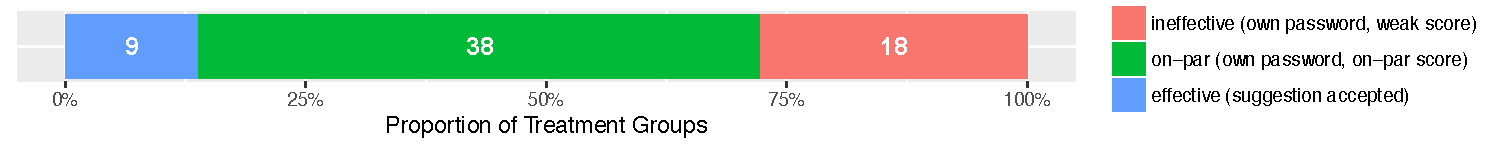
\includegraphics[width=\linewidth]{decoy/treatment-impact-edited}
	\caption{\label{fig:decoy:treatment-impact-edited} Nudge efficacy in treatment groups (n=65)}
\end{figure}
Across all treatment groups, nine respondents out of 65 ($\approx$ 14\%) accepted a suggested password verbatim -- four in the Passphrase group, two in the Mangled group, and three in the Decoy group (two targets, one decoy). Suggestions were thus effective for one in ten participants. From the remaining 56 self-selected passwords, 18 (27.7\%) were weaker than the suggestions. In other words, the nudge was ineffective for roughly a third of participants judged by their choice to pick a password that was weaker than the suggestion. For the remaining 38 participants (58.4\%), the nudge could have influenced them to create passwords that as strong as the suggestions, but we lack data to investigate this. Figure \ref{fig:decoy:treatment-impact-edited} visualizes the efficacy of suggesting passwords.

\subsubsection{Impact on Password Strength}
Table \ref{tbl:decoy:zxcvbn-m-sd} lists descriptive statistics on password strength metrics. Taking the entire sample into account, omnibus tests did not show significant differences between the four groups. However, we plotted the confidence intervals of all metrics to examine the data visually. Here, it is visible that guess numbers did notably differ between the groups: the Passphrase treatment led to the strongest passwords overall (see Figure \ref{fig:decoy:ci-guesses-all}). If we remove the samples where a suggestion was accepted, the differences become smaller (see Figure \ref{fig:decoy:ci-guesses-own}). Since guess numbers are shown on a logarithmic scale, the difference appears might appear smaller than it actually is: guess numbers in the passphrases group were about 50 times higher than in the control and mangled groups. This is also visible in Figure \ref{fig:decoy:guess-number-plot}, where the percentage of cracked passwords is consistently smaller than in the other groups. Fitting a smoothed generalized additive model to the cracked percentages confirms that passwords are less likely to be cracked after any given number of guesses, if they were created in the Passphrase condition ($intercept=Control,B=-7.9\%, p<0.001$. \Rsqadj{0.99}). The rise in strength most likely is due to increased password length in the Passphrase group, see Figure \ref{fig:decoy:ci-length-own}.

\begin{table}
  \centering
  \caption{\label{tbl:decoy:zxcvbn-m-sd}Summaries of password metrics from the online experiment. Arranged by group (columns) and metric (rows)}
    \begin{tabular}{p{2cm}rr|rr|rr|rr}
    \toprule
          & \multicolumn{2}{c}{\textbf{Control}} & \multicolumn{2}{c}{\textbf{Mangled}} & \multicolumn{2}{c}{\textbf{Passphrase}} & \multicolumn{2}{c}{\textbf{Decoy}} \\
    \midrule
          & \multicolumn{1}{c}{M} & \multicolumn{1}{c}{SD} & \multicolumn{1}{c}{M} & \multicolumn{1}{c}{SD} & \multicolumn{1}{c}{M} & \multicolumn{1}{c}{SD} & \multicolumn{1}{c}{M} & \multicolumn{1}{c}{SD} \\
    length & 11.33 & 3.53  & 11.8  & 2.74  & 13.87 & 3.8   & 11.9  & 2.69 \\ 
    score & 2.88  & 1.02  & 2.9   & 0.76  & 3.29  & 0.9   & 2.95  & 0.88 \\
    guesses$_{log10}$ & 8.84  & 2.41  & 8.86  & 2.15  & 13.48 & 7.63  & 10.12 & 4.85 \\
    digits & 2.61  & 2.06  & 2.28  & 1.27  & 2.16  & 2.18  & 2.6   & 2.34 \\
    special & 0.22  & 0.64  & 0.52  & 1.16  & 0.2   & 0.5   & 0.3   & 0.57 \\
    uppercase & 1.77  & 0.8   & 1.42  & 0.59  & 2.45  & 2.35  & 1.75  & 1.11 \\
    lowercase & 6.55  & 3.91  & 7.38  & 3.21  & 8.91  & 4.09  & 6.95  & 3.42 \\
    \bottomrule
    \end{tabular}%
\end{table}%

%None of the participants' passwords was scored as ``very weak'' (0). 

\begin{figure}
	\centering
	\begin{subfigure}[c]{0.45\textwidth}
		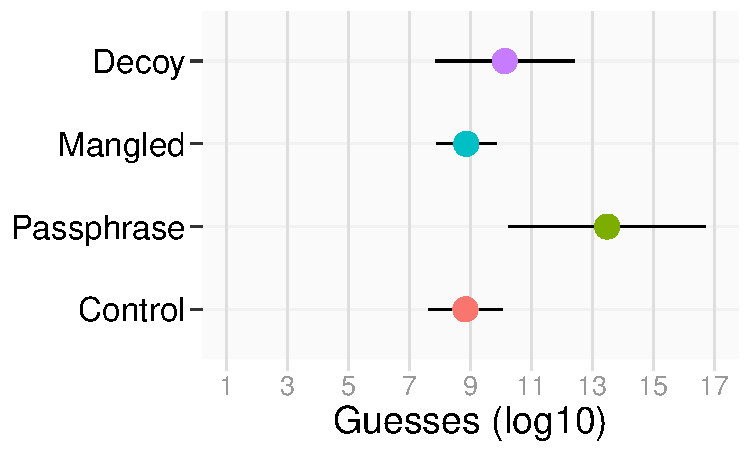
\includegraphics[width=\textwidth]{figures/decoy/ci-guessesLog10-all}
		\caption{\label{fig:decoy:ci-guesses-all} Confidence intervals of estimated guess-numbers (log 10) for all participants (N=83). On average, the Passphrase group created significantly stronger passwords than the Control and Mangled group.}
	\end{subfigure}
	\begin{subfigure}[c]{0.45\textwidth}
		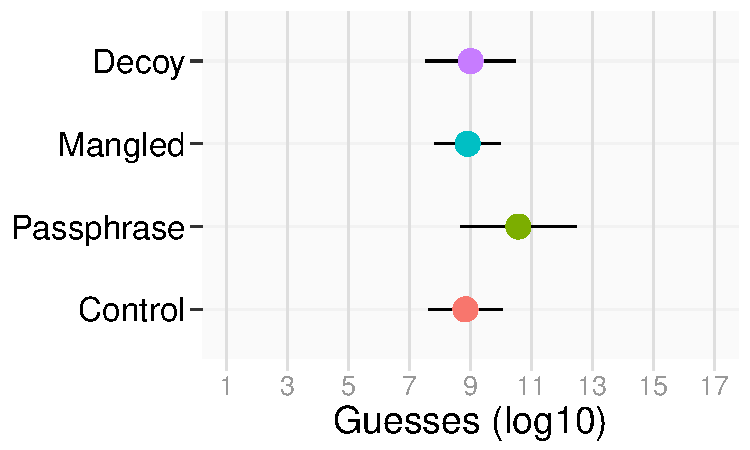
\includegraphics[width=\textwidth]{figures/decoy/ci-guessesLog10-own}
		\caption{\label{fig:decoy:ci-guesses-own}
			Confidence intervals of estimated guess-numbers (log 10) for self-selected passwords (N=74). Although the difference between the Passphrase group and the others is not as big as in the overall sample, the average guess numbers are still $\approx$ two orders of magnitude apart.}
	\end{subfigure}
	\caption{\label{fig:decoy:results-strenth} Arithmetic mean of guess numbers (log 10) and 95\% confidence intervals.} 
\end{figure}

\begin{figure}
	\centering
	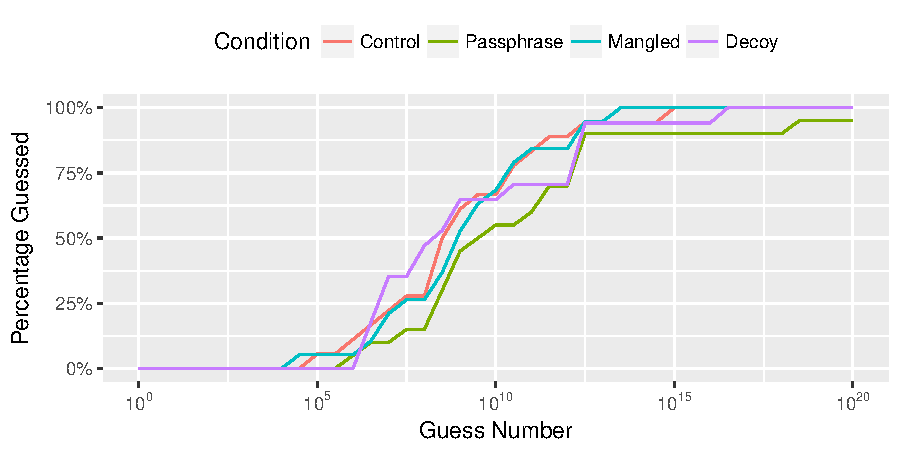
\includegraphics[width=0.8\linewidth]{decoy/guess-number-plot}
	\caption{\label{fig:decoy:guess-number-plot} Estimated guessability of user-selected passwords across the four conditions.}
\end{figure}

\begin{figure}
	\centering
	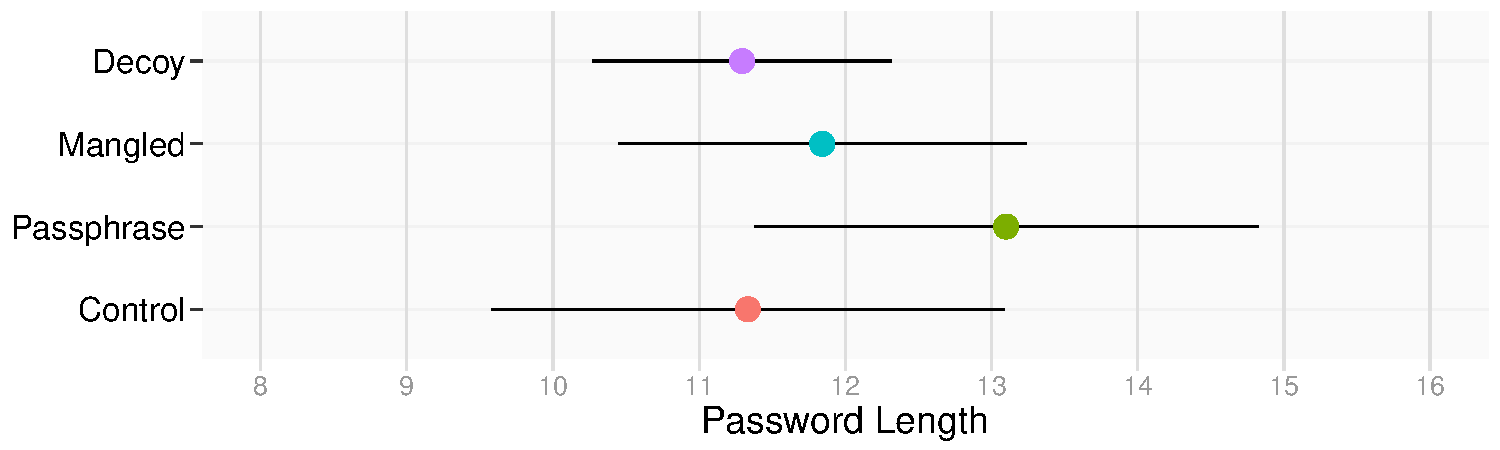
\includegraphics[width=0.8\linewidth]{decoy/ci-length-own}
	\caption{\label{fig:decoy:ci-length-own} Average password length of self-selected passwords and 95\% confidence intervals}
\end{figure}

%\subsection{Live-Deployment Data}
%Talk about a couple of findings of the Roskilde dataset. 
% nah. there's no time for that now. 
%TODO add screenshot from roskilde sign-up. 

\subsubsection{Password Composition and Policy Adherence}
\begin{table}
  \centering
  \caption{\label{tab:decoy:policies}Policy fulfillment of submitted passwords. Most participants used at least three character classes.}
    \begin{tabular}{rrrrrrrr}
    \toprule
          & \begin{turn}{45}comp8\end{turn} & \begin{turn}{45}3class8\end{turn} & \begin{turn}{45}3class12\end{turn} & \begin{turn}{45}3class16\end{turn} & \begin{turn}{45}basic8\end{turn} & \begin{turn}{45}basic12\end{turn} & \begin{turn}{45}basic16\end{turn} \\
    \midrule
    Control     & 2     & 9     & 4     & 0     & 1     & 1     & 1 \\
    Mangled    & 6     & 7     & 3     & 3     & 1     & 1     & 0 \\
   Passphrase   & 4     & 5     & 4     & 2     & 1     & 1     & 7 \\
    Decoy    & 5     & 7     & 3     & 1     & 1     & 1     & 2 \\
    \midrule
    $\Sigma$  & 17    & 28    & 14    & 6     & 4     & 4     & 10 \\
    \bottomrule
    \end{tabular}%
\end{table}%%tab:decoy:policies%
It is possible to sort participants' self selected passwords into ``policy buckets'', i.e. the most stringent policy they would fulfill. This makes the effort to create a stronger password visible. Table \ref{tab:decoy:policies} shows the distribution of this analysis in commonly used policy taxonomy \cite{Shay2014CanLongPasswordsBeSecureAndUsable}. 
A chi-squared test showed no significant differences across groups ($\chi^2(18)=16.93,p>0.5$). Yet, it is interesting that even though only a basic8 policy was enforced, all participants formed passwords with at least two character classes. The majority (78\%) even used three character classes. Participants in the Mangled condition were about twice as likely to adhere to one of the complex policies (comp8, 3class12, 3class16) than the Control group. On average, the length requirement was exceeded by $\approx 4$ characters. 

\subsubsection{Memorability}
Roughly 40\% ($n=34$) of participants succeeded to provide their password from the first part of the study. A chi-squared test on group differences was not significant ($\chi^2(3)=3.84,p>0.05$). Among the participants whose passwords matched three days later, 76\% ($n=26$) reported to have memorized it, while the rest had their browser store it (2), or put it into a digital file (5) or on paper (1). Participants who had opted for a suggestion were mostly unable to authenticate. A respondent in the Decoy group correctly entered the mangled password in the second part, reportedly from memory. %TODO Conclusion: accepting suggestions seems to be coupled with the assumption that passwords are not required to memorize: Accept suggestion = use password manager in the users mental model. Would change if suggestions need to be typed.

\subsubsection{Qualitative Findings \& Feedback}
A thematic co-analysis of the qualitative data collected at the end of both study parts, there were no observable differences, therefore we do not report group-specific details.  %Figure \ref{fig:prolific_likert_all} shows the the most relevant subjective ratings. 

In the three treatment groups, we elicited data on the subjective perceptions of the suggestions. Participants were shown adjectives from which they could select multiple items and provide additional text. The most common reactions were ``neutral'' ($n=25$), ``surprised'' ($n=23$) and ``pleased'' ($n=11$). There was no observable tendency as to perceived security improvements for email accounts by the suggestions. 20 participants (24\%) might be annoyed if their main email provider implemented a sign-up form like the one in the study, but they did not clarify this further. 30 respondents (36\%) acknowledged that suggestions could facilitate email account creation. The main reason to decline the suggestions was the need for passwords with personal meanings (43\% agreement rate). 
%new
Besides, P81 said that ``the main reason I don't use generated passwords, is that if a hacker finds out how they're generated, they've basically figured everyone's passwords out. Then its only a matter of time before they brute force into accounts using the same method the system uses to generate them.'' This quote highlights the distrust regarding password generators, while at the same time assuming attackers are incapable of predicting human behavior.
% memo
Finally, there were interesting qualitative statements about the memorability of passwords (all \textit{sic}): ``sorry, i would have written it down if i knew there was a second part to the study. thats what i do for passwords that i will use again, until i memorize it, then i throw away the paper i write it on.'' (P33) ``I'm not sure if it was because I don't type this password I used here often or if it [is] because I used one of my lesser very weak passwords that I failed to remember it quickly. Regardless, I need a few better habits. '' (P26) ``I forgot my password as I didn't think I'd need it again. Had I known I would likely have tried harder to remember it.'' (P47). From these statements, we take away three important points: a) Some participants were unaware that they would need the password in the future, b) they rely on their own memorization techniques, and c) they feel guilty of bad password habits which echoes the results in Chapter \ref{chap:mm_pwm}. In summary, those factors had contributed to the low memorability rates of the study passwords. 

\subsection{Limitations}
There are a few important aspects to consider in the interpretability of our study findings. The sampling method, although state of the art, still targets users who are open-minded enough to participate in studies. Only those crowd-workers with a successful track record were screened in, thus the sample might not be representative for the entire population. However, rough trends can be seen in any case. In terms of sample size, we had initially hoped for a larger data set, but had to omit a significant proportion due to low quality of the data. This leads to a lack of statistical power, which forbids us to narrow down confidence intervals and thus find significant effects. The lack is aggravated by the fact that many study participants chose passwords that were much stronger than what is to be expected from real-world passwords \cite{Mazurek2013Measuring}. Such behavior reduces ecological validity and shrinks potential effect sizes induced by different nudges. Despite these limitations, it is astonishing to still detect notable differences across groups. Finally, we relied on the zxcvbn strength metric, as in many other studies throughout this thesis. We could have collected plain-text passwords and used a more robust approach like PGS \cite{Ur2015MeasuringRealWorldAccuracies}. However, this would have been too risky, because participants might have disclosed their real email passwords in the scenario, which we regard as unethical. Therefore, the zxcvbn metrics are one of the best solutions to work around this issue while providing sufficient robustness.

\section{Discussion}

\subsection{The Ineffectiveness of the Decoy Effect}
- users were still unaware of the two dimensions: usability and security. the ease of use was still too low to compete against their own passwords. 
- the original experiments were within subjects. counterbalanced order. start out with three options --> two in the second part and vice versa. maybe this could have helped bring forward the desired nudging effect. 

reject H2, support H1

\subsection{Creativity Support}
As we have seen in chapter \ref{chap:pasdjo}, users know fairly well what makes a strong password. Thus, we can explain the stronger influence of the passphrase in several ways. There might be a gap between password strength perception and selection that is due to \textit{creativity}. It might be easier for people to decide upon a stronger password if they actually see it. This, however, will not work, if the password is absolutely unrelated to the person because this increases memorization efforts. 

Creativity is usually associated with the ``Openness'' personality trait (see chapter \ref{chap:pws_and_personality}). So we can suspect that people who show less of this trait might be more susceptible to a password suggestion. 

accept suggestion --> need password manager.

mental model influenced? -- look at qualitative data. 


\begin{figure}
	\centering
	\includegraphics[width=0.7\linewidth]{figures/decoy/expire_mockup}
	\caption{\label{fig:decoy:expiremockup}Suggestion accompanied by enforced password expiration information.}
\end{figure}


\subsection{Application Areas}
it is not feasible to make users pick strong passwords for all accounts.
they already keep a list of ``important'' accounts that they wish to protect well, but stay in charge, so picking a strong memorable password for this type of account is vital to them. 

also, master passwords as gate-keeper to a larger number of passwords. 

\subsection{Personas}
which personas might be most most receptive to suggestions?

\section{Conclusion}

The idea we put forward in \cite{Seitz2016DecoyEffect} (see Figure \ref{fig:decoy:expiremockup}) was very recently evaluated by Renaud and Zimmermann \cite{Renaud2018NudgingFolks}. They concluded that providing a graspable benefit is the key to effectively nudge users towards stronger passwords. 

%Future Work

\vspace*{2cm}\noindent
\fbox{
	\hspace{1cm}
	\parbox[c][8cm]{0.7\linewidth}{
		\section*{Take Aways}
		\begin{itemize}[leftmargin=*]
			\item Users can identify weak passwords, but overestimate the strength of mangled passwords.
			\item Passphrases are seen as weak, but it is possible to influence users' mental models with persuasive design.
			\item A game-based approach is feasible to collect data inexpensively.
		\end{itemize}
	}
	\hspace{1cm}
}

 %published
%TODO put this into the final discussion at the end.
%\chapter[Side-Effects and Corroborative Results]{Side-Effects and Corroborative Results}\label{chap:side_effects}


%Corroborative 
\section{What users do to create strong passwords}
- Hier alles zusammenfassen was in den Studien herausgefunden wurde, 
was Leute tun, um starke Passwörter zu generieren. 
- In alle BAs/ MAs reinschauen weil da jeder etwas dazu geschrieben hat. 



% New anecdotal or unanticipated findings



 


\part{THE PASSWORD SUPPORT TOOLKIT}
%!TEX root = ../../psst.tex

\chapter[Overview]{Overview}\label{chap:psst_overview}

The Password Selection Support Toolkit (PSST) is a holistic approach to help users of any experience level manage their password portfolio of any size. Ideally, continuous usage of the PSST enables and encourages users to 
\begin{enumerate}
\item[a)] improve their strategies
\item[b)] strengthen the passwords
\item[c)] boost memorability of passwords
\end{enumerate}
All this leads to an improvement of user experience as both pragmatic and hedonic qualities are maximized. 

\section{Privacy Concerns}
To make sure users can fully benefit from the power of the PSST, it is required that no information about the user's behavior travels through the web, i.e. to remote servers. Such knowledge would deeply compromise protection against foreign access. Attackers would intensify attacks on the stored behavioral data that would allow them to reverse engineer credentials. This has to be avoided at all costs. Consequently, the calculations need to take place on the client-side. With increasing computational power even for consumer electronic devices this does not seem to be a tough restriction. 

\section{Adapting to Existing Strategies}
As discussed in Chapter \ref{sec:password_selection}, each individual user handles password selection and memorization differently, even though patterns occur. 

The most prevalent factors for password selection are:
\begin{itemize}
\item Account Value
\item Memorability
\item \textbf{Perceived Strength}. As we have seen, people's perception of strength has changed, so as to speak ``they were enlightened''. Everyday practice has taught users that difficult passwords are good, but everybody thinks that they seem hard to do. The PSST allows to shift this perception. 
\end{itemize}

The PSST lets the user know, that their strategy is legitimate. It acknowledges them and does not want to change them.  Even password re-use can be beneficial.

The PSST addresses password strategies, by learning them through both active involvement and observation. 

\subsection{Learning Account Values}
The PSST adjusts nudges and persuasion to the users' perceived value of a password. 

\subsubsection{Measuring Password Value}
Users often fail to assess the value of passwords correctly as we have seen in (@TODO REF SEC). 

\section{Composition Policy Fulfillment}

\section{Supporting Memorization}
After the users picked their password, be it completely independently or with aid by the PSST, they are now facing the critical stage of memorizing it. In case they simply re-used or modified an old password, this phase is very short. They might write down which of their ready-made credentials they utilized. This is necessary and helpful if the account value is not clear or might change in the future. 

However, in case the PSST manage to persuade a user towards are slightly different option than they would have chosen without it, memorization is extremely important. As such, the PSST provides means to support this process in @TODO ways:
\begin{itemize}
\item training. 
\item \textbf{Storing}. The password is stored and can be retrieved from a local database. 
\end{itemize}

\section{Hedonic Qualities}
Hedonic UX qualities are often overlooked. The design and incorporates them from the very beginning. 




\chapter[Proof-of-Concept: Password Reuse Manager]{Proof-of-Concept: Password Reuse Manager}\label{chap:pwrm}

\section{Background and Context}
Password managers (PWMs) are one of the common coping strategies for an ever growing number of accounts. 
% übergang zu dem noch ausformulieren. 
Zhang-Kennedy \etal provided a detailed literature review on common recommendations for users \cite{ZhangKennedy2016RevisitingPasswordRules}. They come to the conclusion that reuse is not necessarily bad. In fact, they provide an updated recommendation that to ``\textit{\textbf{strategically}} reuse passwords''. Moreover, Wash \etal stated that ``defining appropriate categories of websites for re-use of passwords of varying strengths is an open area of research;'' \cite{Wash2016UnderstandingPasswordChoices}. In this chapter, we report on the design, implementation, and basic evaluation of a password manager that incorporates the notion of secure strategic password-reuse. The chapter is partially based on a Bachelor thesis by Magdalena Sifferlinger, a Master Thesis by Martin Prinz, and a technical report by Anabelle Bockwoldt, Dimitri Reisler, and Julia Speckmeier. All these works were carried out under my supervision and guidance. \ar

\subsection{Conceptual Idea}
Security-wise it is recommendable to have a unique, strong password for every account, but as discussed in detail in Section \ref{sec:rw:user-behavior}, the reality looks different, because user's are overwhelmed with the task. At the heart of this work, we embrace user behavior as it is and do not try to ``fix the user''. We design for current user behavior first, and apply nudging techniques later. This is the notion of \textit{supporting} password coping strategies, rather than \textit{fixing} them. 


A number of studies has highlighted that users reuse passwords \ar. Virtually every user has developed their personal reuse strategy either independently, or after receiving advice by peers or the media. For instance, people mentally put accounts in categories  like ``important account'' and ``throwaway account'' \cite{Egelman2013DoesMyPasswordGoUpToEleven}. Others might have created a mangling scheme based on the purpose of the password. Our password manager aims to support users to continue using their strategy even with the password manager, but potentially in a smoother way. One of our goals is to eventually lower the barrier of adopting a password manager, because only around 12\% of (American) users rely on a password manager


\subsection{Research Objectives and Contribution}
\textbf{Design an implementation of paradigm-shifting password manager}


\textbf{Platform for user studies}

\textbf{Open Source Password Manager}
Extensible, security audits, visually appealing design. Software that goes beyond simple prototype.

\subsection{Related Work}
Maqbali and Mitchell talk about a reuse algorithm implemented in their ``AutoPass'' prototype \cite{Maqbali2016PasswordGenerators}.
``site-specific'' pseudorandom passwords

``Password managers often have poor support for roaming and inadequately studied usability [3].'' \cite{Herley2012PersistenceOfPasswords}

\section{Design Iterations and Evaluations}

\subsection{Low-Fidelity Prototyping and Pre-Studies}
% essentially magdalena sifferlinger's work here.
Research Questions: which strategies to users utilize to categorize passwords?
method: two-tiered: online study (N=35) and personal semi-structured interviews on the street (N=5). 


\subsection{Persuasive Patterns in Popular Password Managers}
% ath stuff here.
We conducted an analysis about which persuasive patterns can be found in password managers. The analysis served as a basis for some design decisions for the password reuse manager. 

\paragraph{Method}
To do that, we took a list of persuasive patterns \footurl{http://ui-patterns.com/patterns}{02.01.2018}

\subsection{Persuasive Design Elements}

\paragraph{Personalization}
\paragraph{Security Feedback}


other candidates: set completion, value attribution, recogntion over recall, kairos, feedback loops, 

\paragraph{Results}

\section{Field Study}
\subsection{Prototype}
%add some screenshots here
\subsection{Sample}
\subsection{Results}

\section{Discussion}
Suggestion of password categories -- can we use the decoy effect here?

\section{Future Work}
\section{Conclusion}



%\chapter[Policy Fulfillment]{Policy Fulfillment}\label{chap:psst_policy_fulfillment}


\section{Case Study: The Golden Password}
Disclaimer:
The project was carried out in cooperation with Manuel Hartmann, Jakob Pfab, and Samuel Souque. I had the original idea and supervised the project. The students developed the methodology, tested the policies and finally implemented the evaluation web site. 
\subsection{Goals}
\subsection{User Study}
\subsubsection{Methodology}
\subsection{Policy Evaluation Tool}

%\chapter[Passwords -- A User Perspective]{Passwords -- \\
	A User Perspective}\label{chap:rw:user_perspective}
%lingo: arduous

``but his thoughts were so full of the great riches he should possess, that he could not think of the word to make it open, but instead of `Sesame,' said, `Open, Barley!' and was much amazed to find that the door remained fast shut. He named several sorts of grain, but still the door would not open, and the more he endeavoured to remember the word `Simsim,' the more his memory was confounded, and he had as much forgotten it as if he had never heard it mentioned.'' (Kasim's predicament in \textit{Ali Baba and the Forty Thieves}) \todo{this could be the opening of the chapter / fancychapter}

Morris and Thompson were already concerned with user behavior regarding passwords in 1979 \cite{Morris1979PasswordSecurity}. They identified that users choose predictable passwords and that this can be leveraged for attacks. So, they suggested enforcing a certain minimum password length (six characters). At the time, the users were mostly professionals that received training to operate computers and could thus also have been trained to pick less predictable passwords \cite{Maguire2012YouOnlyLiveTwice}. But as computers were introduced to a larger audience, more people were exposed to password authentication. Naturally, this also induced a growing number of attacks, and it is increasingly difficult for users to defend themselves against them (see. Section \ref{sec:rw:attack_vectors}). Nowadays, password policies are in place that require not only a minimum of eight characters, but also mandate mixed-case letters, digits and special symbols to start with. The HCI community noticed the users' struggle in the 1990s and that we can -- and should -- design authentication systems with usability in mind. Perhaps, one of the breaking points where a new school of thought turned up in the literature was a paper by Adams and Sasse in 1999 \cite{Adams1999UsersEnemy}. The central and novel theme in there was a shift from \textit{fixing} the user to \textit{acknowledging} user behavior and designing for it. The paper managed to see over 1500 citations as of writing this.

This chapter looks at the literature that mostly came after this seminal work. It discusses the users' problems, solutions, feelings, and opinions about using passwords. An essential goal is to give the reader an empathetic perspective and provide background information to understand why it seems hard to come up with viable solutions to make users' lives less frustrating. To get there, we first take a brief look at conducting user research with passwords. Hereafter we disseminate typical coping strategies and solutions. The chapter concludes with a comment on the discourse that has been going on between the very different schools of thought about passwords. 

%Each person who gets in contact with the Internet will at some point create a password.

% Everyone develops their own strategy how to do this and how to cope with passwords, probably already in early teenage years \cite{VonZezschwitz2013SurvivalShortest}. These strategies however are not unique and show macroscopic commonalities, which became evident after the first large-scale password leaks. 

%Important: Under coping strategy, we also understand the selection process, because choosing a weak password over a strong one is also one way to \textit{cope} with the large number of passwords and the memorability burden. (make sure to mention this in the general introduction already.)



%@@TODO cite Wash paper @SOUPS 2016.

\cite{Bailey2014StatisticsReuse,Bojinov2010KamouflagePWM,Bonneau2015SecretsLies,Brown2004GeneratingPWs,Chiasson2009InterferencesGraphical,Conklin2004PWAuthenticationSystemPerspective,CSID2012PasswordHabits,Das2014TangledWeb,Dourish2004UserStrategiesEveryday,Florencio2014PasswordPortfoliosFiniteUser,Forget2015CYOA}
\cite{Gaw2005ReuseRecycle,Gaw2006PasswordManagement,Habib2017Blacklists,Haque2014Hierarchy,Hayashi2011DiaryStudyPWs,Huha2015UserReplaceablePasswords,Ives2004DominoEffectReuse,Katsini2017StrategiesGraphicalPasswords,Keith2009PassphraseDesign,Komanduri2011OfPasswordsAndPeople,Kothari2017PasswordLogbooks,Kuo2006HumanSelectionMnemonic,Li2017,Loutfi2015PasswordsOtherSideOfTheFence,Lyastani2016PWMangling,Notoatmodjo2007,Peisert2013PriciplesAuthentication,Riley2006WhatUsersKnowWhatTheyDo}
\cite{Shay2014ReligiousAunt,Shay2010EncounteringPasswordRequirements,Singh2007PasswordSharing,Stobert2014a,Stobert2015,Stobert2014PWMThatDoesntRemember,Stobert2014PasswordLifeCycle,Stobert2015ExpertPassword}
\cite{Ur2015PWCreationLab,Bruggen2013ModifiyngUnlockingBehavior,Veras2012VisualizingSemanticsPasswords,Wang2015ChinesePWs,Wash2016UnderstandingPasswordChoices,Yang2016MnemonicSentenceBased,ZhangKennedy2016RevisitingPasswordRules}




\section{Methodology: Running Password Studies}

general overview a la. how to run a good password study 

\cite{Krol2016ExperimentDesign,Peer2017,Consolvo2003,Ross2010,Sotirakopoulos2011,Oppenheimer2009InstructionalManipulationChecks,Harbach2016HardLockLife,Barbera2013,Carreras2013,Chamberlain2012ResearchInTheWild,Henze2013EmpiricalResearchUbiquitous,Kuhn1993,VonZezschwitz2013SurvivalShortest,Hassenzahl2003,Mazurek2013Measuring,Egelman2015a,Rosoff2014,Savage2012}


Methods:
\begin{itemize}
	\item Analyzing leaked data \cite{Veras2012VisualizingSemanticsPasswords}
	\item Lab study \cite{Sotirakopoulos2011}
	\item Field study only with Logging \cite{Florencio2007LargeScaleStudyPasswordHabits}
	\item Field study with an interactive prototype, often in conjunction with a survey / Diary 
	\item café study  \cite{VonZezschwitz2013SurvivalShortest}
	\item Mechanical Turk / CrowdSourced 
	\item diary study, e.g. \cite{Hayashi2011DiaryStudyPWs}
	\item Triangulation (survey, log analysis) \cite{Wash2016UnderstandingPasswordChoices}
\end{itemize}

all but the first allow controlled selection of passwords

Example: 
Flor\^{e}ncio and Herley probably conducted the largest study to date on password habits. Their intention was to find out among other things A) how often people type passwords, B) how many sites share a password C) how many distinct passwords a user has, and D) how the strong the passwords are. They utilized the Windows Live Toolbar for Internet Explorer to collect in-the-wild data from up to 500000 users during three months of running the collection

\cite{Florencio2007LargeScaleStudyPasswordHabits}. The established protected password lists (PPL) to avoid intruding into people's privacy. They found that users had about 7 distinct passwords in 2007, and that passwords are re-used at about 6 sites in average. Interestingly, they found that stronger passwords are not re-used as often as weak passwords (only around 4 sites). It was not possible to trace the incoming data back to a specific user, which might have resulted in over counting of entries. Also, it was not measured how long the actual password entries takes. If users only used regular dictionary words without any modification, the key logging module of the toolbar would record a password reuse event (PRE) every time the user entered the word -- also in regular text searches, for example. Another limitation could be that they used entropy as a proxy for password strength. However, as discussed in the previous chapter, we have seen that this metric is more robust for system-generated passwords and that strength estimation has evolved over the past ten years. 

Qualitative studies:
Adams Sasse 1997 \cite{Adams1997MakingPWsSecureAndUsable}
Weirich on Persuasion \cite{Weirich2001PrettyGoodPersuasion, Weirich2005PersuasivePasswordSecurity}

Quantitative: 
Yan 2004 Memorability \cite{Yan2004PasswordMemorabilitySecurity}

Position Papers:
Ives Domino Effect \cite{Ives2004DominoEffectReuse}

In the workplace: \cite{Adams1997MakingPWsSecureAndUsable, Inglesant2010TrueCostOfUnusablePolicies}


\todo{Add a table with advantages and disadvantages of different study methods.}


	\subsection{Ecological Validity}
		
 as we have seen before, the approaches differ especially in the way ecological validity is achieved.
 
 ``Ideally, password studies would be conducted by collecting data on real passwords created by real users of a deployed system.'' \cite{Komanduri2011OfPasswordsAndPeople}
 
 explain why ecological validity is super important in this context.
 
 most important papers: 
 many people behave normally, and if you ask them in the survey if they did, this can improve the quality of the data drastically \cite{Fahl2013EcologicalValidityPasswordStudy}
 
 \cite{Krol2016ExperimentDesign}
	
	
	There's a Scale that we can use to cheaply measure security intentions so we can better weight study data from individuals \cite{Egelman2015SeBIS}
	SeBIS is a useful tool and looks robust, but it might need more time to really be considered highly valid \cite{Egelman2016BehaviorEverFollows}

	\subsection{Ethics}
	look into ``Critical'' folder on mendeley
	
	issues:
	\begin{itemize}
		\item collecting plain text passwords - people sometimes
		\item finding efficient ways to attack passwords - this might also help attackers. 
		\item sometimes researchers ``phish'' participants to obtain their passwords (\cite{Egelman2013DoesMyPasswordGoUpToEleven, Haque2014Hierarchy, Mazurek2013Measuring}) -- to conceal the study purpose and get ecologically valid passwords. 
	\end{itemize}
	

	\subsection{Mechanical Turk Studies}
	
	propagated and most commonly used at CMU e.g. \cite{Mazurek2013Measuring} \cite{Shay2014CanLongPasswordsBeSecureAndUsable} \cite{Shay2016DesigningPasswordPolicies}
	\cite{Shay2015UsablePoliciesMTurk}
	\cite{Ur2016PerceptionsPassword} \cite{Melicher2016UsabilityMobileTextPasswords} \cite{Ur2017DataDrivenPWMeter}
	problem: in europe it's not immediately possible, but there are alternatives. 
	
	\cite{Huha2015UserReplaceablePasswords}

	
\section{User Behavior Regarding Passwords}\label{sec:rw:how-users-cope}


\todo{add a table that has all problems on one side and the possible user coping strategies on the other side.}

Take human factors into account when you design secure systems \cite{Sasse2005UsableSecurityPosition}

\cite{Adams1999UsersEnemy} is considered the mother of all HCI \& USEC papers. -- but there were many others before that.

``The main weakness in any password system is that users often choose easily guessable passwords: English words, names, trivial extensions to English words, etc., because they are easy to remember'' from \cite{Feldmeier1990UnixPasswordSecurity},

also 


``password overload'' and ``memory interference'' as technical terms must appear here (for discussion see \cite{Yang2016MnemonicSentenceBased}).


password mechanisms and their users are a socio-technical system and the social aspect weighs heavy \cite{Weirich2001PrettyGoodPersuasion}

Security is too hard for end-users and we need to make it more usable. (fair enough it was the early days of USEC) \cite{Dourish2004UserStrategiesEveryday}

insights into the password burden and context information where people log in, categorization of accounts \cite{Hayashi2011DiaryStudyPWs}


a formal model of the Password Life Cycle, codebook for coping strategies \cite{Stobert2014PasswordLifeCycle}.

\subsection{Selecting Weak Passwords}

	pass\textit{word} implies it has to be a word. Other names for the concept, but basically the same meaning: security code, passcode, secret, credentials, access token
	
	\cite{Jakobsson2013BenefitsUnderstandingPWs}
	
	People show predictable modification behavior \cite{Gaw2005ReuseRecycle}
	
	
	a lot of RockYou's passwords are based on dates and this can be visualized and used for attacks \cite{Veras2012VisualizingSemanticsPasswords}
	
	Greek users do not behave differently than the rest, but the top 100 passwords are a bit different \cite{Violettas2014PasswordsAvoidGreece}

	\subsubsection{Why do Users Select Weak Passwords?}
	
	Users act insecurely because they choose weak passwords that they reuse \cite{Riley2006WhatUsersKnowWhatTheyDo}
	
	people don't take password policies at organizations seriously.  \cite{Weirich2005PersuasivePasswordSecurity}
	
	- policies allow it (\cite{Seitz2017PoliciesReuse})
	- wrong mental model or misinterpretation of security advice (\cite{Ur2015PWCreationLab, Ur2016PerceptionsPassword, Seitz2017PASDJO})
	- because they don't care
	- ... they underestimate the threat
	- ... they are right to judge the account as low value (who would hack me?) \cite{LastPass2016PersonalitiesGetUsHacked}
	
	Passphrases are super predictable because most people use common phrases \cite{Bonneau2012LinguisticProperties}
	
	
	qualitative studies \cite{Ur2015PWCreationLab, Stobert2014PasswordLifeCycle} 
	quantitative studies \cite{Ur2016PerceptionsPassword, Seitz2017PASDJO}
	
	
	Text entry under lab conditions for multiple password selection tasks in a row doesn't have a large effect on typical password metrics \cite{Yang2014EntryAffectsPasswordSecurity}
	
	input modality can be a strong influence on password selection in that mobile devices will lead to less diverse passwords \cite{VonZezschwitz2014HoneyIShrunkTheKeys}
	
	Users understand quite a bit about password security, but we should help them how attacks work \cite{Ur2016PerceptionsPassword}
	
	
	Users are not too bad at creating strong passwords, but often they misinterpret security advice which leads to weak password practices \cite{Ur2015PWCreationLab}
	
	\subsubsection{What's the Problem with Weak Passwords?}
	usually, people tend to use stronger PWs for important accounts
	
	Stronger passwords are not always necessary, do not force users to waste effort. \cite{Florencio2007DoStrongWebPasswords}	


	\subsection{Password Reuse}
	too many accounts problem.
	
	People reuse their passwords and show predictable modification behavior \cite{Gaw2005ReuseRecycle}
	
	The burden of passwords was relatively high in 2007, people reuse passwords \cite{Florencio2007LargeScaleStudyPasswordHabits}
	
	finite effort, and the payoff is invisible (comparison to smoking: I won't be affected, and in many cases that's true. But if you are affected you regret your behavior. )
	
	reuse is the most convenient way but probably the most severe threat to one's online identity and finances. This is a hard problem. 
	
	it's not just the passwords, it's also the user name 
	
	frequently entered passwords are reused more often \cite{Wash2016UnderstandingPasswordChoices} -- but there are contradictory results on this matter. -- Stobert and Biddle argue in the other direction \cite{Stobert2014PasswordLifeCycle}. 
	
	reuse statistic overview of different papers: \cite{Wash2016UnderstandingPasswordChoices} in the discussion section. 
	
	term that you read ever so often: users have a ``go-to password'' that they try first
	and then often the policy can make them change another one. But! If the go-to password is strong and has certain characteristics (as is demonstrated in chapter \ref{chap:policies-reuse}), reusing this is possible and its threats perhaps underestimated. 
	
	\textbf{What's the problem?}
	consequences: phishing attacks are problematic because of the domino effect (Ives \etal) Password reuse is difficult to defend against and we should look into understanding user behavior better \cite{Ives2004DominoEffectReuse}.
	
	but reuse isn't bad per se, it's necessary \cite{Florencio2014PasswordPortfoliosFiniteUser, ZhangKennedy2016RevisitingPasswordRules}. 
	
		
	Users try to prioritize stronger passwords as reuse candidates, and this also means that users try to follow security advice (they belief strong passwords are more important than unique passwords) \cite{Wash2016UnderstandingPasswordChoices}.
	
	
	It's enough to know one low-value password that you mangle to crack a large part of high-value passwords \cite{Haque2014Hierarchy}
	
	
	\subsubsection{Reuse Strategies}
	address the role of policies (see \cite{Seitz2017PoliciesReuse}).
	
	Participants rely on their memory, but reuse passwords, and they have a suboptimal mental model of how attacks work \cite{Gaw2006PasswordManagement}
	
	Users don't care if an account is financial or not, as long as it's perceived as high value, they reuse the password for that \cite{Bailey2014StatisticsReuse}
	
	password reuse is common and modifications are predictable, so it's easy for attackers to optimize their attacks with knowledge from leaked credentials of a specific account \cite{Das2014TangledWeb}

	Password Categories -- arch over to mental accounting from behavioral economics -- \cite{Thaler2004}
	
	Experts have certain articulate strategies to select and manage their passwords, and their situation awareness lets them judge important and non-important accounts more consistently  	\cite{Stobert2015ExpertPassword} 

	Categorization: 
	compare password categorization to mental accounting, then we can cite \cite{Stockinger2015TowardsBE}
	
	category: depending on policies. \cite{Stobert2014PasswordLifeCycle}
	
	
	Coping with passwords by choosing weak passwords and reusing them is absolutely necessary, the problem is how to do it right \cite{Florencio2014PasswordPortfoliosFiniteUser}.
	
	
	A new scale and insights into password support. Password hierarchy \cite{Haque2015PhdProposal}
	
	\subsection{Tools (Writing Down)}
	\cite{Herley2012PersistenceOfPasswords} is in favor of writing down IF the location is secure enough.
	
	Users struggle to manage passwords, but are unfamiliar with supporting tools, so they have developed elaborate strategies to cope \cite{Stobert2014Agony}
	
		\subsubsection{Problem: Accessibility for Local Attackers}
Word documents post-its (use a screen shot of french newspaper that was featured on tv and you could see one of their passwords in the back. spouses can access them .	


	\subsection{Fallback Methods}
	Click on ``forgot'' password basically every time - to avoid this, some services mainly rely on one time passwords, because users are going to forget theirs anyway. 


	\subsection{Account Sharing}
	Account sharing is very common and often necessary, while current designs do not take this behavior into account \cite{Singh2007PasswordSharing}


\section{The Role of Mobile Devices}
touch some small aspects, especially Melicher's Paper \cite{Melicher2016UsabilityMobileTextPasswords} and \cite{VonZezschwitz2014HoneyIShrunkTheKeys}
\cite{Haque2014PsychometricsStrongPassword} 

talk about the rise of graphical and biometric authentication. 


set the stage for the emoji passwords later. 



%%%%%%%%%%%%%%%%%%%%%%%%%
%%%%%
%%%%% COUNTERMEASURES
%%%%%
%%%%%%%%%%%%%%%%%%%%%%%%%
\section{Countermeasures}

if we must keep the human in the loop, e.g. because constraints dictate so, we need to support them well and carefully \cite{Cranor2008FrameworkReasoning}

Usable security shouldn't only be done for end users but also for the people who implement security systems \cite{Acar2016NotYourDeveloper}


	\subsection{Password Composition Policies}
	
	the idea of policies dates back to the 70s: Morris and Thompson suggested to make users
	either choose longer passwords or assign passwords to them \cite{Morris1979PasswordSecurity}
	
	%Lingo: Adhere to a policy
	
	
	Weir \etal categorize policies into ``explicit'' and ``implicit'' policies \cite{Weir2010MetricsPolicies}, where explicit policies have predefined rules about the password structure (e.g. LUDS policy). Implicit policies are based on the estimated strength and are somewhat more volatile and intransparent to the users. Example: blacklist only becomes visible once the user tries to pick a password that's contained in the list. There are also ``external'' policies where the user's password is automatically changed by the system to add some randomness
	
	
	LUDS as a key term \cite{Wheeler2016zxcvbn}
	
		
	Range of Policies as shown by Shay \cite{Shay2014CanLongPasswordsBeSecureAndUsable}
	definitely mention: 28.0\% of passwords in comp8 fulfilled the symbol requirement only by placing ``!'' at the end and using no other symbols. 
	
	\cite{ZhangKennedy2016RevisitingPasswordRules}
	
	
	Workplace-focused: 
	a postulation that password policies should be based on HCI principles rather than security considerations alone. The idea of a holistic password policy is put forward \cite{Inglesant2010TrueCostOfUnusablePolicies} 
	and \cite{Zakaria2013DesigningEffectiveSecurityMessages}
	
	Don't try to fix the user, fix the system first, especially do not impose strict requirements and nonsensical policies \cite{Florencio2014AdministratorsGuide} 
	
	\cite{Ur2015PWCreationLab}
	
	\cite{Shay2010EncounteringPasswordRequirements}
	
	Most detailed insights into effects of password policy design we have to date, password substring blacklist suggestion \cite{Shay2016DesigningPasswordPolicies}
	
	\cite{Weir2010MetricsPolicies}
	
	\cite{Wang2015EmperorsPolicies}
	
	
	\cite{Florencio2010WhereDoPoliciesComeFrom}
	
	\cite{Horsch2016PasswordPolicyMarkup}
	
	\cite{Chiasson2015QuantifyingExpiration}
	\cite{Blocki2013OptimizingPasswordPolicies}
	
	Early comparison of the effects of policies on \textit{human} password selection by Komanduri \etal
	\cite{Komanduri2011OfPasswordsAndPeople}
	
	
	Shay tried to come up with an algorithm that lets administrators decide which policy to use \cite{Shay2009PolicySimulation}.
	
	basic16, 3class12, and 2word16 seem like the winners in terms of security and usability, but persuasion can help to diversify the themes for word-based passwords \cite{Shay2014CanLongPasswordsBeSecureAndUsable}

	\subsection{Advice and Guidelines}
	
	there is a plethora of advice and guidelines out there, but it's not all the same \footurl{https://www.ncsc.gov.uk/guidance/helping-end-users-manage-their-passwords}{22.12.2017}
	
	education in password matters only has so much effect. 
	\cite{Forget2007HelpingUsers} says that even instructions don't work
	
	There's some work that argues that users want to create stronger passwords at least for some accounts, but they had
	misinterpreted security advice. 
	this is also reflected in \cite{Ur2016PerceptionsPassword}
	
	Great overview and critical discussion: \cite{ZhangKennedy2016RevisitingPasswordRules}
	
	
	make it persuasive \cite{Zakaria2013DesigningEffectiveSecurityMessages}
	
	In privacy: people's mental models about privacy are vague and we can see it in their drawings/explanations that they're somewhat overly pessimistic and that education plays the major role \cite{Kang2015MentalModelsDrawing}
	
	
	Stay realistic about password requirements and user effort \cite{Florencio2016CommACM}
		
	
	\subsection{Offering Memorization Techniques}
	
	
	early approaches: random but pronounceable passwords. (good overview in \cite{Kuo2006HumanSelectionMnemonic})
	
	\cite{Bonneau2014ReliableStorage56Bits}
	\cite{Forget2007HelpingUsers}
	
	It might be worthwhile to add a gamification layer onto password managers if you want to memorize some of your most important passwords \cite{Kroeze2012GamifyingAuthentication}\\
	
	\paragraph{Mnemonics}
	Using contextual cues related to a website to base a mnemonic PW on might make them more memorable \cite{Mcevoy2016ContextualizingMnemonicPhrase}
	
	\paragraph{Passphrases}
	(\todo{maybe even merge this with subsection on advice})
	Advantages: PW scheme doesn't have to be changed, people are generally familiar with the concept of passwords, better to enter on virtual keyboards, e.g. TVs (although we don't have any data for that, but that's okay because passwords play a minor role (but still exist there)).
	
	Mnemonic phrase based passwords are strong and memorable \cite{Yan2004PasswordMemorabilitySecurity}.
	
	
	
	Disadvantages: more typos (can be relieved by displaying the password in plain text  \cite{Melicher2016UsabilityMobileTextPasswords}), user choice often predictable
	
	users might not even understand what you want from them if you say they should create a password based on a phrase \cite{Forget2007HelpingUsers}
	
	\cite{Bonneau2012LinguisticProperties}: passphrases already deployed in PGP, Caine and Abel password leak \cite{Carnavalet2014AnalyzingPWStrengthMeters} 
	
	\cite{Shay2012CorrectHorseBatteryStaple}
	
	
	\paragraph{Pronounceable Passwords}
	pronounceable passwords are useful, but we don't know the best way to generate them \cite{Goldberg2015UnspeakablePasswords}
	
	
	\subsection{Password Meters and Real-Time Feedback}
	
	\todo{Define what we mean by password meter} Because some papers don't differentiate between the meters, verbal feedback, suggestions, and real-time feedback on policy fulfillment. (this will be good to show with examples from the real world.)
	
%	Shay \etal say that real-time feedback is not part of the password meter \cite{Shay2015SpoonfulOfSugar}
	
	
	History: zxcvbn paper has some intel on early work on proactive password checks (in the 80s) \cite{Wheeler2016zxcvbn}. specifically (from 1995) \cite{Bishop1995ProactivePasswordChecking}
	
	
	pro-active checks -- dictionary checks Shay argues in favor of dictionary checks \cite{Shay2014CanLongPasswordsBeSecureAndUsable} 
	black lists \cite{Habib2017Blacklists} 
	
	spoonful (guidance) \cite{Shay2015SpoonfulOfSugar}
	\cite{Forget2008ImprovingPasswordsThroughPersuasion}
	
	be careful not to talk too much about persuasion in this chapter. 
	
	We should consider social nudges in usable security, too \cite{DiGioia2005SocialNavigationUsableSecurity}
	
	\subsection{Password Managers}
	
	list all the pro's and con's of PWMs here in different dimensions, e.g. security and usability, kind of similar to \cite{Bonneau2012ReplacePasswords}
	
	
	
	%% from SOUPS MM Poster
	We situate our work in understanding user behavior and attitudes regarding passwords. Here, large parts of the literature focus on \textit{coping strategies} that emerge with a growing number of accounts \cite{Florencio2007LargeScaleStudyPasswordHabits, Florencio2014PasswordPortfoliosFiniteUser}. For example, Stobert and Biddle conducted qualitative analyses to formalize the way users live with their passwords (the ``Password Life Cycle") \cite{Stobert2014PasswordLifeCycle}. This model depicts how users choose, commit, reuse, and reset their passwords. Their work also delivers valuable insights into memorization and organization strategies: Users have mental lists of passwords, e.g. a list for important accounts or a list per website topic. Without explicitly mentioning, the findings contribute to a mental model of password reuse. This is important, because reuse is one of the most common coping strategies \cite{Das2014TangledWeb, Gaw2006PasswordManagement, Hayashi2011DiaryStudyPWs} and many researchers discourage it, because a breach at one site can compromise many others \cite{Bonneau2012ScienceOfGuessing, Komanduri2011OfPasswordsAndPeople}. 
	
	To facilitate coping with passwords and possibly minimize reuse, dedicated tools have been investigated and proposed. Besides industry-driven password managers, HCI research has proposed a number of alternatives. For instance, Stobert and Biddle also propose a password manager that is designed to boost trust as it does not directly store passwords, but rather offers a image cues to recall passwords \cite{Stobert2014PWMThatDoesntRemember}. 
	
	Finally, other researchers followed a mental model approach to understand how users make sense of security mitigations. For instance, Kang et al. utilized drawing tasks to establish users' mental model of data disclosure on the Internet \cite{Kang2015MentalModelsDrawing} to find guidelines for more privacy-sensitive solutions. Bravo-Lillo et al. focused on creating a mental model of security warnings \cite{BravoLillo2011WarningsMentalModel} to improve their framing and timing.
	
	
\section{The Passionate Discourse About Passwords}\label{sec:rw:passionate_discourse}
talk about how critical and passionate this topic has been debated in the literature

--> surprisingly, a lot of position papers (sometimes pure argumentation, sometimes with mathematical/logical reasoning) 

Address Herley's, Florencio's, Sasse's work here. 

e.g. Counterfactuals, Bullying, Finite Effort 


\part{CONCLUSION}
\chapter[Summary]{Summary}\label{chap:summary}



\section{Classification and Dimensions}
here we talk about in which way the projects contributed to the PCT and in which way


\section{Lessons Learned}
What would I do differently the next time I take on a PhD project?




%!TEX root = ../../diss.tex

\chapter[Limitations and Future Work]{Limitations and Future Work}\label{chap:limitations_future_work}


\section{Limitations}


\section{Future Work}

Maybe merge this with Chapter \ref{chap:pst:ideas} (Wild Ideas)


%!TEX root = ../../diss.tex

\chapter[The End - A Sermon]{The End - A Sermon}\label{chap:the_end_old}


Lorem Epson. 

\begin{figure}[htpb]
	\centering
	\includegraphics[width=0.3\linewidth]{shaming/nakedsecurity-sophos}
	\includegraphics[width=0.3\linewidth]{shaming/nytimes}
	\includegraphics[width=0.3\linewidth]{shaming/trusted-reviews}
\end{figure}

Key thoughts

\begin{itemize}
\item Passwords are bad. Let's hope passwords vanish at some point. Make machines intelligent enough to decide if a user should be granted access or not. But this brings new problems.
\item Maybe passwords are the vinyl records of usable security - everyone agrees that it's kind of an obsolete technology but there's something to it that ensure they don't disappear. %TODO come up with a better analogy.
 \item  if passwords become obsolete tomorrow, many of us will not grief. 
 \item  the media should stop shaming the users 
 \item  it's okay to forget passwords! reference to the article Franziska shared with me (SZ,  01.12.2017 ``Die Kunst zu vergessen'' \footurl{http://www.sueddeutsche.de/wissen/neurowissenschaft-die-kunst-zu-vergessen-1.3772438}{02.01.2018}.)
 \item 	ad networks for webpages can undermine any attempt to secure one's account. Too many websites show ads that can run harmful scripts. yes, adblockers do prevent this, but not everyone has one installed (especially novice users don't). Frightening research on this: \footurl{https://freedom-to-tinker.com/2017/12/27/no-boundaries-for-user-identities-web-trackers-exploit-browser-login-managers/}{02.01.2018}
\end{itemize}

It's interesting that often the same idea pops up every other year. so although there are no replication studies, evaluating the same idea multiple times with different setups and specifics, kind of goes in that direction. 


%TODO I have more thann 100 ``takeaways'' from papers. This could be a funny ``sermon'' too (Luther's 100 theses);




% ################################################### MAIN PART

%____________________________________________________________
\cleardoublepage

%____________________________________________________________

\backmatter

%____________________________________________________________

\printglossaries

% REFERENCES FORMAT
% References must be the same font size as other body text.
\bibliographystyle{SIGCHI-Reference-Format}
%\bibliographystyle{acm-sigchi-modern}
\bibliography{library}


\cleardoublepage
%\phantomsection
%\addcontentsline{toc}{chapter}{Index}
%\printindex


\end{document}